% 202? - Francisco Fernandez tesis template
%
% https://github.com/fernandezfran/thesis
\documentclass[12pt,spanish,a4paper,twoside]{book}
\usepackage[spanish,es-nodecimaldot]{babel}

% colores nord blues
\usepackage{xcolor}
% \definecolor{mycolor}{RGB}{94, 129, 172} % nord blue
% \definecolor{mylcolor}{RGB}{129, 161, 193} % nord lighter blue
\definecolor{mycolor}{RGB}{31, 119, 180}

% estilo de pagina
%
%% margenes
\usepackage{geometry}
\geometry{
	a4paper,
	total={170mm,257mm},
	left=20mm,
	top=20mm,
}
%
%% Sangría
\setlength\parindent{12pt}
%
%% Interlineado
\usepackage{setspace}
\onehalfspacing
%
%% Palatino font type
\usepackage[T1]{fontenc}
\usepackage{mathpazo}
%
%% poder definir margenes de un parrafo (adjustwidth)
\usepackage{changepage}
%% encabezados de las páginas
\usepackage{fancyhdr}
\pagestyle{fancy}
\fancyhf{}
%
%%% línea horizontal superior
\let\oldheadrule\headrule
\renewcommand{\headrule}{\color{mycolor}\oldheadrule}
\renewcommand{\headrulewidth}{0.8pt}
%
%%% línea horizonal inferior
%\let\oldfootrule\footrule
%\renewcommand{\footrule}{\color{mycolor}\oldfootrule}
%\renewcommand{\footrulewidth}{0.8pt}
%
%%% header
\renewcommand{\chaptermark}[1]{\markboth{#1}{}}
\renewcommand{\sectionmark}[1]{\markright{#1}}
\fancyhead[CE]{\footnotesize\color{mycolor}\normalfont\bfseries\itshape\nouppercase{
    \textsc{\leftmark}}
}
\fancyhead[CO]{\footnotesize\color{mycolor}\normalfont\bfseries\itshape\nouppercase{
    \textsc{\rightmark}}
}
%
%%% footer
\fancyfoot[CE,CO]{\color{mycolor}\bfseries\thepage}
%
%% carátula de capítulo
\usepackage{sectsty}
\usepackage{titlesec}
\titleformat{\chapter}
    [display]
    {\centering\Huge\bfseries\color{mycolor}}
    {\chaptername\ \thechapter}
    {0pt}
    {\huge}
%
%% color de las secciones
\partfont{\color{mycolor}}
\sectionfont{\color{mycolor}}
\subsectionfont{\color{mycolor}}
\subsubsectionfont{\color{mycolor}}
\let\oldtextbf\textbf
\renewcommand{\textbf}[1]{\textcolor{mycolor}{\oldtextbf{#1}}}
%
%% línea horizontal debajo de las secciones
\titleformat{\section}
  {\normalfont\Large\bfseries\color{mycolor}}
  {\thesection}{1em}{}[{\titlerule[0.8pt]}]
%
%% index
\usepackage{imakeidx}
\makeindex[columns=3, title=Alphabetical Index, intoc]
%
%% show subsubsections in TOC
\setcounter{tocdepth}{4}
\setcounter{secnumdepth}{4}
%
%% Bibliografía por capítulo
\usepackage{tocbibind}
% \usepackage[square,numbers,sort,sectionbib]{natbib}
% \usepackage{chapterbib}
%% para que las citas no rompan el renglón
\usepackage[square]{natbib}
\renewcommand{\cite}{\citep}
%% defino pagina en blanco
\newcommand\blankpage{%
    \null
    \thispagestyle{empty}%
    \addtocounter{page}{-1}%
    \newpage
}

% para borrar los items de itemize
\renewenvironment{itemize}{
\begin{list}{}{
\setlength{\leftmargin}{1.5em}
}
}{
\end{list}
}

% para, desde el índice, poder clickear a que página ir
%\usepackage[obeyspaces]{url}
\usepackage[breaklinks=true,hidelinks]{hyperref} 

% \say para las comillas
\usepackage{dirtytalk}

% para agregar imagenes (includegraphics)
\usepackage{graphicx}
% espeficicando el path de las imagenes, que se repetiría en todas las entradas
% especifico paths desde acá
\graphicspath{{./}}
% subfiguras, definidas en columnas, por ej
\usepackage{subcaption}

% para algunos símbolos en las ecuaciones
\usepackage[fleqn]{amsmath}  % fleqn = flush left equations
\setlength{\mathindent}{24pt}

% tabla en vez de cuadro
\usepackage[tableposition=top, labelfont={color=mycolor,bf}]{caption}
\addto\captionsspanish{
    \def\listtablename{\'Indice de tablas}%
    \def\tablename{Tabla}
}
%
%% para poder separar los títulos en dos renglones
\usepackage{adjustbox}\usepackage{mathtools}
\usepackage{array}
\usepackage{makecell,booktabs}
\usepackage{stackengine}
\setstackEOL{\cr} %EOL is abbreviation for "end of line."

% para acomodar mejor las posiciones de figuras/tablas
\usepackage{float}

\usepackage{colortbl}
\arrayrulecolor{mycolor}

% para agregar código Python
\usepackage{listings}

\definecolor{code-green}{RGB}{44, 160, 44}
\definecolor{code-magenta}{RGB}{227, 119, 194}

\lstdefinestyle{mystyle}{
    backgroundcolor=\color{white},
    commentstyle=\color{code-magenta},
    keywordstyle=\color{mycolor},
    stringstyle=\color{code-green},
    basicstyle=\ttfamily\footnotesize,
    breakatwhitespace=false,
    breaklines=true,
    captionpos=b,
    keepspaces=true,
    numbersep=5pt,
    showspaces=false,
    showstringspaces=false,
    showtabs=false,
    extendedchars=true,
    tabsize=4
}

\lstset{
    style=mystyle,
    literate=
    {á}{{\'a}}1
    {é}{{\'e}}1
    {í}{{\'i}}1
    {ó}{{\'o}}1
    {ú}{{\'u}}1
}


\begin{document}

% enumeración de las primeras páginas con números romanos
\frontmatter

% \blankpage
% \blankpage

% Carátula
\thispagestyle{empty}
\begin{center}
{\large

    \vspace{1cm}

    {\Huge Estudios experimentales y teóricos para el desarrollo de electrodos 
    de baterías de ion-litio de próxima generación}
    
    \vspace{0.5cm}
    por
    \vspace{0.5cm}
    
    {\Large Francisco Fernandez}

    \vspace{0.5cm}

    Presentado ante la Facultad de Matemáticas, Astronomía, Física y Computación 
    como parte de los requerimientos para la obtención del grado de
    
    \vspace{0.5cm}

    {\Large Doctor en Física}

    \vspace{0.5cm}
    de la

    UNIVERSIDAD NACIONAL DE CÓRDOBA

    \vspace{0.5cm}
    % logo 
    
    mes, 202?

    \textcopyright FaMAF - UNC 202?

    \vspace{1.5cm}

    Director: Daniel Eugenio Barraco Díaz

    Codirector: Ezequiel Pedro Marcos Leiva

    % licencia
}
\end{center}

% Dedicatoria

% Índice
\tableofcontents
% \listoffigures
% \listoftables

% Resumen

% Abstract

% a partir de acá se cuentan los números de las páginas en formato arabico
\mainmatter

% Capítulos

%\part{Motivación y fundamentos}
%
%\section{Introducción}

%
%\section{Métodos computacionales}

\subsection{Cálculos DFT}\label{s:dftcalc}

Los cálculos de DFT de las estructures cristalinas fueron obtenidos usando el 
paquete de simulación \path{GPAW} \cite{enkovaara2010, mortensen2005} del 
Entorno de Simulación Atómica \cite{larsen2017}. El paquete \path{GPAW} provee un 
algoritmo de grillado del espacio real basado en el método de la función de onda 
aumentada por proyector \cite{blochl1994} que utiliza la aproximación del núcleo 
congelado. Las coordenadas de Li, Li$_{15}$Si$_{4}$, Li$_{13}$Si$_{4}$, 
Li$_{7}$Si$_{3}$, Li$_{12}$Si$_{7}$, LiSi y Si se descargaron del Materials 
Project \cite{materials_project} (códigos mp: 135, 569849, 672287, 1201871, 1314, 
795 y 149) correspondiente al Li BCC, x $\approx$ 3.75, 3.25, 2.33, 1.71, 1 y
Si diamante, respectivamente. Los cálculos DFT se realizaron utilizando el 
funcional de intercambio-correlación PBE (Perdew-Burke-Ernzerhof) y la integración
de la zona de Brillouin se efectuó con grillas Monkhorst-Pack con una densidad
de 2.5 puntos $k$ por \AA$^{-1}$.

También se estudiaron, con cálculos DFT, estructuras amorfas de Li$_x$Si siguiendo
el protocolo de litiación propuesto por Chevrier y Dahn \cite{chevrier2009, 
chevrier2010}. Se utilizó un esquema de celda repetida con 12 átomos de silicio y 
$N$ de litio por celda unidad, con $N\in[0,45]$ cubriendo todo el intervalo 
$x\in[0,3.75]$. Cada estructura Li$_{N+1}$Si$_{12}$ se obtuvo agregando un átomo 
de litio en la esfera vacía más grande de la celda Li$_{N}$Si$_{12}$ y realizando
una optimización geométrica de las posiciones atómicas y del volumen de la celda.
En este caso, se realizaron los cálculos con el programa \path{QUANTUM} 
\path{ESPRESSO} \cite{quantum_espresso,quantum_espresso_advanced}, utilizando el 
funcional de intercambio-correlación PBE con una energía cinética de corte de 
1090 eV y una integración de la zona de Brillouin con grillas Monkhorst-Pack con 
una densidad de 7 puntos $k$ por \AA$^{-1}$. Las posiciones atómicas y el volumen 
de la celda se optimizaron utilizando el algoritmo BFGS hasta que la fuerza fuera 
menor a 0.08 eV/\AA\ para cada estructura.


\subsection{Detalles técnicos de DFTB}\label{ss:dftb}

El formalismo de DFTB ya fue introducido en el capítulo \ref{ch:metodos}, 
sección \ref{s:dftb}. A la hora de elegir el potencial de confinamiento de la
ecuación \ref{eq:dft} se mencionó que lo usual es elegir un parabólico, 
cuadrático, o una función de ley de potencias, siendo esta última opción la 
utilizada debido a que es la que está implementada en el código \path{Hotcent}
\cite{hotcent},
\begin{equation}\label{eq:vconf}
    V_{\text{conf}}(r)=\left(\frac{r}{r_0}\right)^{\sigma}
\end{equation}
donde $r_0$ y $\sigma$ son números reales que pueden ser elegidos de para cada 
orbital atómico $\phi$ y cada densidad $\rho^0$.

En la Tabla \ref{t:hubbard} se presentan las configuraciones electrónicas 
utilizadas, junto a las energías en el sitio de los orbitales de valencia y a 
los parámetros de Hubbard calculados, que se introducen en el segundo término
de la ecuación \ref{eq:dftb}.
\begin{table}[h!]
    \centering
    \caption{Configuraciones electrónicas, energías en el sitio de los orbitales
    de valencia y parámetros de Hubbard calculados con el funcional de intercambio
    y correlación PBE.}
    \setlength\extrarowheight{2pt}\stackon{%
    \begin{tabular}{l c c c c c}
        \toprule
        \textbf{Elemento} & 
        \textbf{Capa de valencia} &  
        \textbf{$\varepsilon_s$} &
        \textbf{$\varepsilon_p$} &  
        \textbf{$U_s$} & 
        \textbf{$U_p$} \\
        \midrule
        Li & 2s$^1$ & -0.105127 & -- & 0.167057 & -- \\
        Li & 3s$^2$3p$^2$ & -0.395452 & -0.150169 & 0.329247 & 0.244483 \\
        \bottomrule
    \end{tabular}
    }{}
    \label{t:hubbard}
\end{table}

El potencial de repulsión utilizado para definir la ecuación \ref{eq:rep} 
se ajustó utilizando el código \path{TANGO} \cite{tango}, donde el potencial 
repulsivo está dado por:
\begin{equation}\label{eq:v_rep}
    V_{\text{rep}}(r) = \begin{cases}
        e^{-a_1r+a_2}+a_3 & 0\le r<r_{\min}\\
        \displaystyle\sum_{i=2}^m c_i\left(r_{\text{cut}}-r\right)^i & r_{\min}\le r < r_{\text{cut}}\\
        0 & r_{\text{cut}} \le r
    \end{cases}
\end{equation}
los valores que se utilizan para $r_{\min}$ y $r_{\text{cut}}$ se encuentran
en la Tabla \ref{t:mincut}. Los parámetros $a_i$ se ajustan para reproducir las 
energías de DFT para cada estructura elegida para el entrenamiento utilizando el 
algoritmo de Levenber-Marquardt. Se eligió el grado del polinomio $m = 8$ y 
los coeficiente $c_i$ se optimizaron con un ajuste por cuadrados mínimos.

\begin{table}[h!]
    \centering
    \caption{Valores de $r_{\min}$ y $r_{\text{cut}}$ utilizados en la ecuación
    \ref{eq:v_rep}}
    \setlength\extrarowheight{2pt}\stackon{%
    \begin{tabular}{l c c}
        \toprule
        & 
        \textbf{$r_{\min}$ [\AA]} & 
        \textbf{$r_{\text{cut}}$ [\AA]} \\
        \midrule
        Si-Si & 1.7760 & 3.4410 \\
        Si-Li & 1.7925 & 4.1825 \\
        Li-Li & 1.9456 & 4.7360 \\
        \bottomrule
    \end{tabular}
    }{}
    \label{t:mincut}
\end{table}

Los códigos \path{Hotcent} y \path{TANGO} proveen valores por defecto para 
cualquier otro parámetro que no haya sido explícitamente descripto. 


\subsection{Algoritmo de ajuste}\label{s:algfit}

Para la obtención de los parámetros Li-Si de DFTB se siguió el 
método de aprendizaje descripto en los trabajos de van den Bossche \textit{et al.}
\cite{van2018, van2019}. Esto se realizó para dos conjuntos de parámetros, 
denotados como conjunto A y conjunto B, que difieren entre ellos en el ajuste
del término de la energía de bandas. En el conjunto A se ajusta la estructura 
de bandas de Li y Si por separado, mientras que en el conjunto B se utiliza para 
esto la estructura Li$_7$Si$_3$. La elección de esta última estructura se debe a
que el valor para la energía de formación es el menor entre todas las aleaciones
cristalinas consideradas \cite{materials_project}. La parametrización de los 
orbitales pseudoatómicos y de las densidades electrónicas consisten en optimizar 
los valores de $r_0$ y $\sigma$ en la ecuación \ref{eq:vconf} para ajustar la 
estructura de bandas de referencia de DFT. La Tabla \ref{t:vconf_params} muestra
los valores de los parámetros de confinamiento optimizados.
\begin{table}[h]
    \centering
    \caption{Parámetros del potencial de confinamiento $r_0$ y $\sigma$ para 
    los orbitales atómicos $\phi$ y las densidades $\rho^0$ de Li y Si}
    \setlength\extrarowheight{2pt}\stackon{%
    \begin{tabular}{l ccccc ccccc}
        \toprule
        &\multicolumn{5}{c}{\textbf{conjunto A}}&\multicolumn{5}{c}{\textbf{conjunto B}}\\
            \textbf{Elemento} & \textbf{$r_0(\phi)$} & \textbf{$\sigma(\phi)$} & \textbf{$r_0(\rho^0)$} & \textbf{$\sigma(\rho^0)$} & & & \textbf{$r_0(\phi)$} & \textbf{$\sigma(\phi)$} & \textbf{$r_0(\rho^0)$} & \textbf{$\sigma(\rho^0)$}\\
        \midrule
         Li & $4.899$ & $1.889$ & $7.233$ & $1.986$ & & & $4.843$ & $1.927$& $7.210$ & $1.999$\\
         Si & $4.558$ & $6.909$ & $6.318$ & $2.188$ & & & $3.556$ & $2.382$& $6.292$ & $1.891$\\
        \bottomrule
    \end{tabular}
    }{}
    \label{t:vconf_params}
\end{table}

Por otro lado, el conjunto de datos de entrenamiento requerido para ajustar el 
término de repulsión de pares se obtuvo utilizando las estructuras cristalinas 
ya mencionadas. Llámese $S$ al conjunto de estructuras cristalinas. A cada una de 
ellas se le realizaron compresiones y expansiones isotrópicas utilizando un 
factor de escaleo que varió de 0.4 a 1.45 con un equiespaciado de 0.05 unidades, 
generando así 22 estructuras por estequiometría. La energía de cada estructura se 
computó con DFT y se descartaron aquellas que superaban los 10 eV del mínimo de 
la estequiometría. De este procedimiento se obtuvieron 108 estructuras para el 
conjunto de entrenamiento. Para cada estructura $s$ de una dada estequiometría 
en $S$ ($s \in S$) se denota por $N_s$ la cantidad de estructuras asociadas a 
ella. Además, para cada estequiometría $s$, se denota con ${\bf r}^s_i$ la 
$i$-esima estructura y con $\check{{\bf r}}^s$ la estructura correspondiente a la
menor energía de DFT. Se usará el símbolo ``$\ \check{\ }\ $'' para denotar 
el argumento del mínimo de otras funciones.

Teniendo esto en cuenta, se obtiene el conjunto de parámetros 
$\check{\bf p} = \left( \left\{\check{c}_i\right\}, \left\{\check{a}_i\right\}\right)$ 
(ver ecuación \ref{eq:rep}) de DFTB que minimizan la sumatoria de los residuos 
de la energía
\begin{equation}\label{eq:e_res}
    \text{Res}_E({\bf p})=\sum_{s\in S}\sum_{i=1}^{N_s} \omega^s_i
    \left[E_{\text{DFT}}({\bf r}^s_i)-(E_{\text{DFTB}}({\bf r}^s_i;{\bf p})-C)\right]^2
\end{equation}
donde $C$ es una constante que desplaza la energía DFTB para corregir tendencias
sistemáticas a sobre- o sub-estimar energías \cite{van2018, van2019}, 
$E_{\text{DFTB}}({\bf r}^s_i;{\bf p})$ es la energía calculada utilizando DFTB con 
el conjunto de parámetros ${\bf p}$, $\omega_i^s$ permite controlar el peso 
relativo de cada estructura ${\bf r}^s_i$ en el proceso de ajuste.

Con el fin de minimizar la ecuación \ref{eq:e_res} es necesario elegir los pesos 
relativos $\omega_i^s$. En la referencia \cite{van2019}, los autores sugieren una 
distribución tipo Boltzmann
\begin{equation}\label{eq:omega}
    \tilde\omega^s_i=\exp\left(-\frac{E_\text{DFT}({\bf r}^s_i)-E_s}{b^s_i}\right)
\end{equation}
donde $b^s_i$ se considera proporcional al número de átomos $n^s_i$ en cada 
estructura y $E_s$ es la energía de referencia. Como se sugiere en la
documentación del código \path{TANGO} \cite{tango}, se puede fijar 
$b^s_i = 0.1 n^s_i$ eV y una elección adecuada para $E_s$ sería la energía más 
baja de la estequiometría $s$
\begin{equation}\label{eq:e_s}
  E_s=E_\text{DFT}(\check{{\bf r}}_s) \leq E_\text{DFT}({\bf r}^s_i) \quad \forall i \in [1,N_s].
\end{equation}
La motivación subyacente para esta ecuación es aumentar la precisión del modelo 
DFTB resultante para predecir estructuras de baja energía, renunciando a tener 
dicha precisión en estructuras de alta energía, que tienen menos probabilidad 
de ser encontradas durante una simulación canónica. Cabe destacar que este factor
de peso sólo se aplica a las estructuras de la estequiometría $s$ y no pesa las 
distintas estequiometrías.

Al elegir los pesos de las estructuras en el conjunto de entrenamiento en la 
ecuación \ref{eq:e_res}, se puede configurar el alcance de la aplicación para 
la parametrización de DFTB resultante. En otras palabras, para cada conjunto de 
pesos hay un conjunto de parámetros de DFTB ($\check{{\bf p}}$) distinto que 
minimiza la ecuación \ref{eq:e_res}. Basándose en esta idea, se puede elegir que 
los pesos sean
\begin{equation}\label{eq:omega2}
      \omega^s_i=\xi_s\tilde\omega^s_i=\xi_s\exp\left(-\frac{E_\text{DFT}({\bf r}^s_i)-E_s}{b^s_i}\right)
\end{equation} 
reteniendo así el enfoque en las estructuras de menor energía para cada 
estequiometría pero incluyendo un nuevo conjunto de coeficientes 
$\boldsymbol{\xi}$ $=\left(\xi_{\text{Li}},\cdots,\xi_{\text{Si}}\right)$ que 
permite controlar el peso relativo entre las distintas estequiometrías. Con esta 
definición, los parámetros óptimos de DFTB para la ecuación \ref{eq:e_res},
$\check{{\bf p}}$, pueden considerarse como una función que depende de 
$\boldsymbol{\xi}$, $\check{{\bf p}}(\boldsymbol{\xi})$. Lo cual 
introduce un segundo proceso de optimización para obtener los coeficientes 
$\check{\boldsymbol{\xi}}$.

El objetivo final de este capítulo es la parametrización de un modelo DFTB que 
permita luego simular la litiación de ánodos de silicio. Este es un proceso muy 
complejo ya que involucra distintos entornos químicos, con un intervalo amplio de
composiciones de Li$_x$Si. Sin embargo, es importante que la parametrización
mantenga su precisión para el mayor rango posible de concentraciones, para evitar 
la necesidad de cambiar de modelo \say{\textit{on-the-fly}} durante una simulación,
por lo que se requiere que la parametrización sea lo más transferible posible 
entre las distintas estequiometrías. En este sentido, el objetivo principal de la 
parametrización es que la misma realice predicciones fiables de algún observable, 
en este caso de las energías de formación relativas por átomo (definidas en la 
ecuación \ref{eq:formacion}) evaluadas en las estructuras 
$\lbrace \check{\mathbf{r}}_s \rbrace$. Por lo tanto, se 
optimizan los valores de los coeficientes $\check{\boldsymbol{\xi}}$ tal que 
minimizan la sumatoria de los residuos de las energías de formación relativas por 
átomo
\begin{equation}\label{eq:fres}
    \text{Res}_F(\boldsymbol{\xi}) = \sum_{s\in S} \left[F_\text{DFT}(\check{{\bf r}}^s)-F_\text{DFTB}(\check{{\bf r}}^s;\check{{\bf p}}({\boldsymbol{\xi}}))\right]^2
\end{equation}
La minimización de este residuo resulta en un conjunto de parámetros de DFTB
$\check{{\bf p}}(\check{\boldsymbol{\xi}})$ óptimo en el conjunto de 
entrenamiento donde las estequiometrías también son pesadas para dar un residuo
mínimo en su energía de formación.

En la Figura \ref{fig:diagrama} se muestra un diagrama de flujo con los pasos 
principales del algoritmo de ajuste descripto arriba. La minimización de la 
ecuación \ref{eq:e_res} se realiza con el código \path{TANGO} \cite{tango}. Para
minimizar la ecuación \ref{eq:fres}, se desarrolló un programa llamado 
\path{Milonga} que ejecuta varias instancias de \path{TANGO}, una por cada
evaluación de Res$_F(\boldsymbol{\xi})$ requerida por el proceso de minimización.

\begin{figure}[h!]
    \centering
    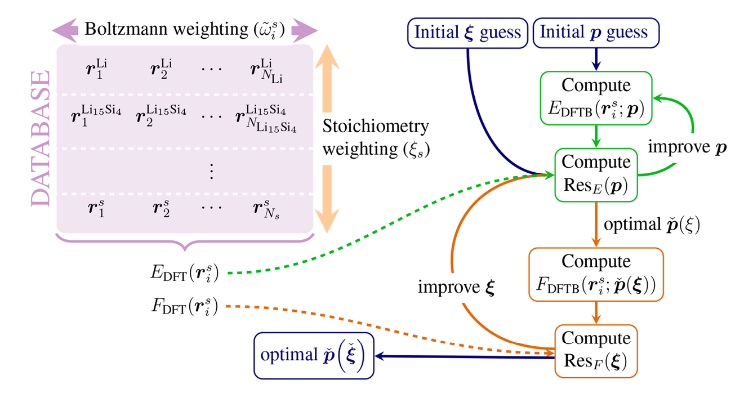
\includegraphics[width=\textwidth]{Silicio/modelo/metodos/diagrama.png}
    \caption{Diagrama de flujo del algoritmo de ajuste. Se realizan dos
    procedimientos de optimización anidados: la minimización de Res$_E$ (ecuación 
    \ref{eq:e_res}) utilizando el código \texttt{TANGO} \cite{tango} (resaltado en
    verde) y la minimización de Res$_F$ (ecuación \ref{eq:fres}) utilizando un 
    código llamado \texttt{Milonga} (resaltado en naranja). Cada mejora de los pesos
    $\boldsymbol{\xi}$ requiere una minimización completa de Res$_E$ para obtener 
    los parámetros óptimos DFTB asociados $\check{{\bf p}}(\boldsymbol{\xi})$.}
    \label{fig:diagrama}
\end{figure}

%

% \part{Carga rápida de baterías de ion-litio}

% % Copyright (c) 2024, Francisco Fernandez
% License: CC BY-SA 4.0
%   https://github.com/fernandezfran/thesis/blob/main/LICENSE
\chapter{Un modelo heurístico basado en simulaciones galvanóstaticas}\label{ch:un}
\thispagestyle{empty}

% \vspace{50pt}

% \begin{adjustwidth}{50pt}{50pt}
%     Una de las características a modificar más importantes para conseguir una mejora de los 
%     vehículos eléctricos, frente a los de combustión interna, es la carga rápida.
%     Con el objetivo de optimizar los materiales activos, en este
%     capítulo se presenta un modelo heurístico que permite encontrar las 
%     condiciones de carga rápida, correspondientes a obtener el 80\% del Estado de la Carga en 15 minutos, de
%     electrodos de una sola partícula de baterías de ion-litio, aprovechando así
%     la máxima capacidad posible. Se propone una guía basada en un modelo general 
%     que considera las limitaciones por la difusión de los iones y por la transferencia de carga interfacial
%     en condiciones de corriente constante. Para la utilización de la misma, se 
%     desarrolló una librería en Python que es de libre acceso y fácil de usar para 
%     realizar el preprocesamiento de datos experimentales y realizar estimaciones.
% \end{adjustwidth}

% \clearpage
% \newpage
% \thispagestyle{empty}
% \mbox{}
% \newpage

\section{Introducción}

\section{Métodos computacionales}

\subsection{Cálculos DFT}\label{s:dftcalc}

Los cálculos de DFT de las estructures cristalinas fueron obtenidos usando el 
paquete de simulación \path{GPAW} \cite{enkovaara2010, mortensen2005} del 
Entorno de Simulación Atómica \cite{larsen2017}. El paquete \path{GPAW} provee un 
algoritmo de grillado del espacio real basado en el método de la función de onda 
aumentada por proyector \cite{blochl1994} que utiliza la aproximación del núcleo 
congelado. Las coordenadas de Li, Li$_{15}$Si$_{4}$, Li$_{13}$Si$_{4}$, 
Li$_{7}$Si$_{3}$, Li$_{12}$Si$_{7}$, LiSi y Si se descargaron del Materials 
Project \cite{materials_project} (códigos mp: 135, 569849, 672287, 1201871, 1314, 
795 y 149) correspondiente al Li BCC, x $\approx$ 3.75, 3.25, 2.33, 1.71, 1 y
Si diamante, respectivamente. Los cálculos DFT se realizaron utilizando el 
funcional de intercambio-correlación PBE (Perdew-Burke-Ernzerhof) y la integración
de la zona de Brillouin se efectuó con grillas Monkhorst-Pack con una densidad
de 2.5 puntos $k$ por \AA$^{-1}$.

También se estudiaron, con cálculos DFT, estructuras amorfas de Li$_x$Si siguiendo
el protocolo de litiación propuesto por Chevrier y Dahn \cite{chevrier2009, 
chevrier2010}. Se utilizó un esquema de celda repetida con 12 átomos de silicio y 
$N$ de litio por celda unidad, con $N\in[0,45]$ cubriendo todo el intervalo 
$x\in[0,3.75]$. Cada estructura Li$_{N+1}$Si$_{12}$ se obtuvo agregando un átomo 
de litio en la esfera vacía más grande de la celda Li$_{N}$Si$_{12}$ y realizando
una optimización geométrica de las posiciones atómicas y del volumen de la celda.
En este caso, se realizaron los cálculos con el programa \path{QUANTUM} 
\path{ESPRESSO} \cite{quantum_espresso,quantum_espresso_advanced}, utilizando el 
funcional de intercambio-correlación PBE con una energía cinética de corte de 
1090 eV y una integración de la zona de Brillouin con grillas Monkhorst-Pack con 
una densidad de 7 puntos $k$ por \AA$^{-1}$. Las posiciones atómicas y el volumen 
de la celda se optimizaron utilizando el algoritmo BFGS hasta que la fuerza fuera 
menor a 0.08 eV/\AA\ para cada estructura.


\subsection{Detalles técnicos de DFTB}\label{ss:dftb}

El formalismo de DFTB ya fue introducido en el capítulo \ref{ch:metodos}, 
sección \ref{s:dftb}. A la hora de elegir el potencial de confinamiento de la
ecuación \ref{eq:dft} se mencionó que lo usual es elegir un parabólico, 
cuadrático, o una función de ley de potencias, siendo esta última opción la 
utilizada debido a que es la que está implementada en el código \path{Hotcent}
\cite{hotcent},
\begin{equation}\label{eq:vconf}
    V_{\text{conf}}(r)=\left(\frac{r}{r_0}\right)^{\sigma}
\end{equation}
donde $r_0$ y $\sigma$ son números reales que pueden ser elegidos de para cada 
orbital atómico $\phi$ y cada densidad $\rho^0$.

En la Tabla \ref{t:hubbard} se presentan las configuraciones electrónicas 
utilizadas, junto a las energías en el sitio de los orbitales de valencia y a 
los parámetros de Hubbard calculados, que se introducen en el segundo término
de la ecuación \ref{eq:dftb}.
\begin{table}[h!]
    \centering
    \caption{Configuraciones electrónicas, energías en el sitio de los orbitales
    de valencia y parámetros de Hubbard calculados con el funcional de intercambio
    y correlación PBE.}
    \setlength\extrarowheight{2pt}\stackon{%
    \begin{tabular}{l c c c c c}
        \toprule
        \textbf{Elemento} & 
        \textbf{Capa de valencia} &  
        \textbf{$\varepsilon_s$} &
        \textbf{$\varepsilon_p$} &  
        \textbf{$U_s$} & 
        \textbf{$U_p$} \\
        \midrule
        Li & 2s$^1$ & -0.105127 & -- & 0.167057 & -- \\
        Li & 3s$^2$3p$^2$ & -0.395452 & -0.150169 & 0.329247 & 0.244483 \\
        \bottomrule
    \end{tabular}
    }{}
    \label{t:hubbard}
\end{table}

El potencial de repulsión utilizado para definir la ecuación \ref{eq:rep} 
se ajustó utilizando el código \path{TANGO} \cite{tango}, donde el potencial 
repulsivo está dado por:
\begin{equation}\label{eq:v_rep}
    V_{\text{rep}}(r) = \begin{cases}
        e^{-a_1r+a_2}+a_3 & 0\le r<r_{\min}\\
        \displaystyle\sum_{i=2}^m c_i\left(r_{\text{cut}}-r\right)^i & r_{\min}\le r < r_{\text{cut}}\\
        0 & r_{\text{cut}} \le r
    \end{cases}
\end{equation}
los valores que se utilizan para $r_{\min}$ y $r_{\text{cut}}$ se encuentran
en la Tabla \ref{t:mincut}. Los parámetros $a_i$ se ajustan para reproducir las 
energías de DFT para cada estructura elegida para el entrenamiento utilizando el 
algoritmo de Levenber-Marquardt. Se eligió el grado del polinomio $m = 8$ y 
los coeficiente $c_i$ se optimizaron con un ajuste por cuadrados mínimos.

\begin{table}[h!]
    \centering
    \caption{Valores de $r_{\min}$ y $r_{\text{cut}}$ utilizados en la ecuación
    \ref{eq:v_rep}}
    \setlength\extrarowheight{2pt}\stackon{%
    \begin{tabular}{l c c}
        \toprule
        & 
        \textbf{$r_{\min}$ [\AA]} & 
        \textbf{$r_{\text{cut}}$ [\AA]} \\
        \midrule
        Si-Si & 1.7760 & 3.4410 \\
        Si-Li & 1.7925 & 4.1825 \\
        Li-Li & 1.9456 & 4.7360 \\
        \bottomrule
    \end{tabular}
    }{}
    \label{t:mincut}
\end{table}

Los códigos \path{Hotcent} y \path{TANGO} proveen valores por defecto para 
cualquier otro parámetro que no haya sido explícitamente descripto. 


\subsection{Algoritmo de ajuste}\label{s:algfit}

Para la obtención de los parámetros Li-Si de DFTB se siguió el 
método de aprendizaje descripto en los trabajos de van den Bossche \textit{et al.}
\cite{van2018, van2019}. Esto se realizó para dos conjuntos de parámetros, 
denotados como conjunto A y conjunto B, que difieren entre ellos en el ajuste
del término de la energía de bandas. En el conjunto A se ajusta la estructura 
de bandas de Li y Si por separado, mientras que en el conjunto B se utiliza para 
esto la estructura Li$_7$Si$_3$. La elección de esta última estructura se debe a
que el valor para la energía de formación es el menor entre todas las aleaciones
cristalinas consideradas \cite{materials_project}. La parametrización de los 
orbitales pseudoatómicos y de las densidades electrónicas consisten en optimizar 
los valores de $r_0$ y $\sigma$ en la ecuación \ref{eq:vconf} para ajustar la 
estructura de bandas de referencia de DFT. La Tabla \ref{t:vconf_params} muestra
los valores de los parámetros de confinamiento optimizados.
\begin{table}[h]
    \centering
    \caption{Parámetros del potencial de confinamiento $r_0$ y $\sigma$ para 
    los orbitales atómicos $\phi$ y las densidades $\rho^0$ de Li y Si}
    \setlength\extrarowheight{2pt}\stackon{%
    \begin{tabular}{l ccccc ccccc}
        \toprule
        &\multicolumn{5}{c}{\textbf{conjunto A}}&\multicolumn{5}{c}{\textbf{conjunto B}}\\
            \textbf{Elemento} & \textbf{$r_0(\phi)$} & \textbf{$\sigma(\phi)$} & \textbf{$r_0(\rho^0)$} & \textbf{$\sigma(\rho^0)$} & & & \textbf{$r_0(\phi)$} & \textbf{$\sigma(\phi)$} & \textbf{$r_0(\rho^0)$} & \textbf{$\sigma(\rho^0)$}\\
        \midrule
         Li & $4.899$ & $1.889$ & $7.233$ & $1.986$ & & & $4.843$ & $1.927$& $7.210$ & $1.999$\\
         Si & $4.558$ & $6.909$ & $6.318$ & $2.188$ & & & $3.556$ & $2.382$& $6.292$ & $1.891$\\
        \bottomrule
    \end{tabular}
    }{}
    \label{t:vconf_params}
\end{table}

Por otro lado, el conjunto de datos de entrenamiento requerido para ajustar el 
término de repulsión de pares se obtuvo utilizando las estructuras cristalinas 
ya mencionadas. Llámese $S$ al conjunto de estructuras cristalinas. A cada una de 
ellas se le realizaron compresiones y expansiones isotrópicas utilizando un 
factor de escaleo que varió de 0.4 a 1.45 con un equiespaciado de 0.05 unidades, 
generando así 22 estructuras por estequiometría. La energía de cada estructura se 
computó con DFT y se descartaron aquellas que superaban los 10 eV del mínimo de 
la estequiometría. De este procedimiento se obtuvieron 108 estructuras para el 
conjunto de entrenamiento. Para cada estructura $s$ de una dada estequiometría 
en $S$ ($s \in S$) se denota por $N_s$ la cantidad de estructuras asociadas a 
ella. Además, para cada estequiometría $s$, se denota con ${\bf r}^s_i$ la 
$i$-esima estructura y con $\check{{\bf r}}^s$ la estructura correspondiente a la
menor energía de DFT. Se usará el símbolo ``$\ \check{\ }\ $'' para denotar 
el argumento del mínimo de otras funciones.

Teniendo esto en cuenta, se obtiene el conjunto de parámetros 
$\check{\bf p} = \left( \left\{\check{c}_i\right\}, \left\{\check{a}_i\right\}\right)$ 
(ver ecuación \ref{eq:rep}) de DFTB que minimizan la sumatoria de los residuos 
de la energía
\begin{equation}\label{eq:e_res}
    \text{Res}_E({\bf p})=\sum_{s\in S}\sum_{i=1}^{N_s} \omega^s_i
    \left[E_{\text{DFT}}({\bf r}^s_i)-(E_{\text{DFTB}}({\bf r}^s_i;{\bf p})-C)\right]^2
\end{equation}
donde $C$ es una constante que desplaza la energía DFTB para corregir tendencias
sistemáticas a sobre- o sub-estimar energías \cite{van2018, van2019}, 
$E_{\text{DFTB}}({\bf r}^s_i;{\bf p})$ es la energía calculada utilizando DFTB con 
el conjunto de parámetros ${\bf p}$, $\omega_i^s$ permite controlar el peso 
relativo de cada estructura ${\bf r}^s_i$ en el proceso de ajuste.

Con el fin de minimizar la ecuación \ref{eq:e_res} es necesario elegir los pesos 
relativos $\omega_i^s$. En la referencia \cite{van2019}, los autores sugieren una 
distribución tipo Boltzmann
\begin{equation}\label{eq:omega}
    \tilde\omega^s_i=\exp\left(-\frac{E_\text{DFT}({\bf r}^s_i)-E_s}{b^s_i}\right)
\end{equation}
donde $b^s_i$ se considera proporcional al número de átomos $n^s_i$ en cada 
estructura y $E_s$ es la energía de referencia. Como se sugiere en la
documentación del código \path{TANGO} \cite{tango}, se puede fijar 
$b^s_i = 0.1 n^s_i$ eV y una elección adecuada para $E_s$ sería la energía más 
baja de la estequiometría $s$
\begin{equation}\label{eq:e_s}
  E_s=E_\text{DFT}(\check{{\bf r}}_s) \leq E_\text{DFT}({\bf r}^s_i) \quad \forall i \in [1,N_s].
\end{equation}
La motivación subyacente para esta ecuación es aumentar la precisión del modelo 
DFTB resultante para predecir estructuras de baja energía, renunciando a tener 
dicha precisión en estructuras de alta energía, que tienen menos probabilidad 
de ser encontradas durante una simulación canónica. Cabe destacar que este factor
de peso sólo se aplica a las estructuras de la estequiometría $s$ y no pesa las 
distintas estequiometrías.

Al elegir los pesos de las estructuras en el conjunto de entrenamiento en la 
ecuación \ref{eq:e_res}, se puede configurar el alcance de la aplicación para 
la parametrización de DFTB resultante. En otras palabras, para cada conjunto de 
pesos hay un conjunto de parámetros de DFTB ($\check{{\bf p}}$) distinto que 
minimiza la ecuación \ref{eq:e_res}. Basándose en esta idea, se puede elegir que 
los pesos sean
\begin{equation}\label{eq:omega2}
      \omega^s_i=\xi_s\tilde\omega^s_i=\xi_s\exp\left(-\frac{E_\text{DFT}({\bf r}^s_i)-E_s}{b^s_i}\right)
\end{equation} 
reteniendo así el enfoque en las estructuras de menor energía para cada 
estequiometría pero incluyendo un nuevo conjunto de coeficientes 
$\boldsymbol{\xi}$ $=\left(\xi_{\text{Li}},\cdots,\xi_{\text{Si}}\right)$ que 
permite controlar el peso relativo entre las distintas estequiometrías. Con esta 
definición, los parámetros óptimos de DFTB para la ecuación \ref{eq:e_res},
$\check{{\bf p}}$, pueden considerarse como una función que depende de 
$\boldsymbol{\xi}$, $\check{{\bf p}}(\boldsymbol{\xi})$. Lo cual 
introduce un segundo proceso de optimización para obtener los coeficientes 
$\check{\boldsymbol{\xi}}$.

El objetivo final de este capítulo es la parametrización de un modelo DFTB que 
permita luego simular la litiación de ánodos de silicio. Este es un proceso muy 
complejo ya que involucra distintos entornos químicos, con un intervalo amplio de
composiciones de Li$_x$Si. Sin embargo, es importante que la parametrización
mantenga su precisión para el mayor rango posible de concentraciones, para evitar 
la necesidad de cambiar de modelo \say{\textit{on-the-fly}} durante una simulación,
por lo que se requiere que la parametrización sea lo más transferible posible 
entre las distintas estequiometrías. En este sentido, el objetivo principal de la 
parametrización es que la misma realice predicciones fiables de algún observable, 
en este caso de las energías de formación relativas por átomo (definidas en la 
ecuación \ref{eq:formacion}) evaluadas en las estructuras 
$\lbrace \check{\mathbf{r}}_s \rbrace$. Por lo tanto, se 
optimizan los valores de los coeficientes $\check{\boldsymbol{\xi}}$ tal que 
minimizan la sumatoria de los residuos de las energías de formación relativas por 
átomo
\begin{equation}\label{eq:fres}
    \text{Res}_F(\boldsymbol{\xi}) = \sum_{s\in S} \left[F_\text{DFT}(\check{{\bf r}}^s)-F_\text{DFTB}(\check{{\bf r}}^s;\check{{\bf p}}({\boldsymbol{\xi}}))\right]^2
\end{equation}
La minimización de este residuo resulta en un conjunto de parámetros de DFTB
$\check{{\bf p}}(\check{\boldsymbol{\xi}})$ óptimo en el conjunto de 
entrenamiento donde las estequiometrías también son pesadas para dar un residuo
mínimo en su energía de formación.

En la Figura \ref{fig:diagrama} se muestra un diagrama de flujo con los pasos 
principales del algoritmo de ajuste descripto arriba. La minimización de la 
ecuación \ref{eq:e_res} se realiza con el código \path{TANGO} \cite{tango}. Para
minimizar la ecuación \ref{eq:fres}, se desarrolló un programa llamado 
\path{Milonga} que ejecuta varias instancias de \path{TANGO}, una por cada
evaluación de Res$_F(\boldsymbol{\xi})$ requerida por el proceso de minimización.

\begin{figure}[h!]
    \centering
    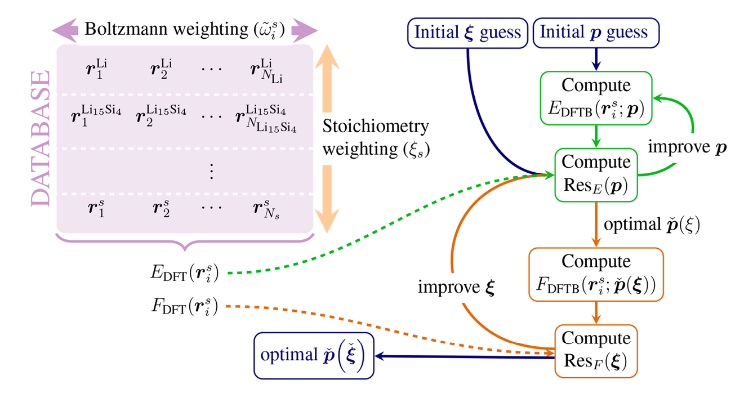
\includegraphics[width=\textwidth]{Silicio/modelo/metodos/diagrama.png}
    \caption{Diagrama de flujo del algoritmo de ajuste. Se realizan dos
    procedimientos de optimización anidados: la minimización de Res$_E$ (ecuación 
    \ref{eq:e_res}) utilizando el código \texttt{TANGO} \cite{tango} (resaltado en
    verde) y la minimización de Res$_F$ (ecuación \ref{eq:fres}) utilizando un 
    código llamado \texttt{Milonga} (resaltado en naranja). Cada mejora de los pesos
    $\boldsymbol{\xi}$ requiere una minimización completa de Res$_E$ para obtener 
    los parámetros óptimos DFTB asociados $\check{{\bf p}}(\boldsymbol{\xi})$.}
    \label{fig:diagrama}
\end{figure}

% \section{Resultados}

\section{Introducción}


\subsection{Comportamiento electroquímico}

\subsubsection{Cambio de volumen fraccionario}

El cambio de volumen fraccionario puede definirse utilizando una normalización 
relativa al número de átomos de Si en la estructura de acuerdo a
\begin{equation}\label{eq:fvc}
    \text{fvc} = \frac{N_{\text{Si}}}{V_{\text{Si}}} \left( \frac{V_{\text{Si},x}}{N_{\text{Si},x}} - \frac{V_{\text{Si}}}{N_{\text{Si}}} \right),
\end{equation}
donde $V_{\text{Si}}$ y $N_{\text{Si}}$ son el volumen y el número de átomos de 
Si en la celda unidad de c-Si, $V_{\text{Si},x}$ y $N_{\text{Si},x}$ son el 
volumen y el número de átomos de Si
en la celda de simulación para el valor correspondiente de $x$. En la Figura
\ref{fig:fvc} se muestran los valores calculados a partir de la ecuación 
\ref{eq:fvc} para las distintas estructuras de Li$_x$Si estudiadas. En la misma 
se comparan los valores obtenidos con datos experimentales de AFM (\textit{atomic 
force microscopy}, sus siglas en inglés) medidos por Beaulieu \textit{et al.} 
~\cite{beaulieu2003} y con predicciones de DFT con un cambio volumétrico fijo 
utilizado por Chevrier y Dahn ~\cite{chevrier2009}. Los mismos muestran que el
potencial ReaxFF proporciona una tendencia correcta, tanto cualitativa como 
cuantitativamente.
\begin{figure}[th]
    \centering
    \includegraphics[width=0.8\textwidth]{Silicio/caracterizacion/resultados/electroquimica/fvc.png}
    \caption{Cambio de volumen fraccionario en función de la composición de la 
    aleación. Los valores experimentales de AFM se muestran con cuadrados azules, 
    la línea recta se corresponde con cálculos de DFT y los círculos rojos son 
    resultados de este trabajo.}
    \label{fig:fvc}
\end{figure}

\subsubsection{Voltaje}

\begin{table}[h]
    \centering
    \caption{Energías de formación obtenidas a través de la ecuación \ref{eq:fe}}
    \setlength\extrarowheight{2pt}\stackon{%
    \begin{tabular}{c c}
        \toprule
        \textbf{x en Li$_x$Si} & 
        \textbf{Energía de formación [eV]} \\ 
        \midrule
        0.21  &  0.503 $\pm$ 0.003 \\
        0.62  &  0.121 $\pm$ 0.007 \\
        1.25  & -0.12 $\pm$ 0.01 \\
        1.71  & -0.236 $\pm$ 0.007 \\
        2.17  & -0.355 $\pm$ 0.008 \\
        2.71  & -0.410 $\pm$ 0.007 \\
        3.25  & -0.52 $\pm$ 0.01 \\
        3.75  & -0.62 $\pm$ 0.01 \\
        4.20  & -0.699 $\pm$ 0.008 \\
        \bottomrule
    \end{tabular}
    }{}
    \label{t:fe}
\end{table}
Las energías obtenidas pueden ser utilizadas para evaluar el funcionamiento del 
modelo para predecir propiedades electroquímicas, como fue sugerido por Chevrier
y Dahn ~\cite{chevrier2009}. Primero, se define la energía de formación de las 
distintas estructuras amorfas como
\begin{equation}\label{eq:fe}
    E_f(x) = E_{\text{Li}_x\text{Si}} - (x E_{\text{Li}} + E_{\text{Si}}),
\end{equation}
donde $E_{\text{Li}_x\text{Si}}$ es la energía de la aleación Li$_x$Si por átomo 
de Si, $E_{\text{Li}}$ y $E_{\text{Si}}$ son las energías cohesivas de Li y Si
en sus fases cristalinas. Usando
la ecuación \ref{eq:fe} como aproximación a la energía de formación de Gibbs, el 
potencial \textit{versus} Li metálico de Li$_x$Si puede obtenerse a partir de
\begin{equation}\label{eq:voltaje}
    V(x) = - \frac{dE_f(x)}{dx},
\end{equation}
donde $V$ es el potencial. Los datos obtenidos así pueden compararse con valores
experimentales y computacionales previos. Las energías de formación calculadas
a partir de la ecuación \ref{eq:fe} se muestran en la Tabla \ref{t:fe}. 
Si se realiza un \textit{spline} a estos valores, mostrados en el recuadro de la
Figura \ref{fig:voltaje}, se obtienen los valores de $V(x)$ a partir de la ecuación
\ref{eq:voltaje}, que se grafican en función de la composición en la Figura 
\ref{fig:voltaje} con una línea roja. Para comparar, se incluye en la misma Figura
las curvas experimentales medidas para la litiación y la delitiación de silicio
amorfo ~\cite{hatchard2004} y la curva teórica de cálculos de primeros principios 
~\cite{chevrier2009}. Se puede afirmar que los resultados obtenidos con el ReaxFF 
son satisfactorios.
\begin{figure}[th]
    \centering
    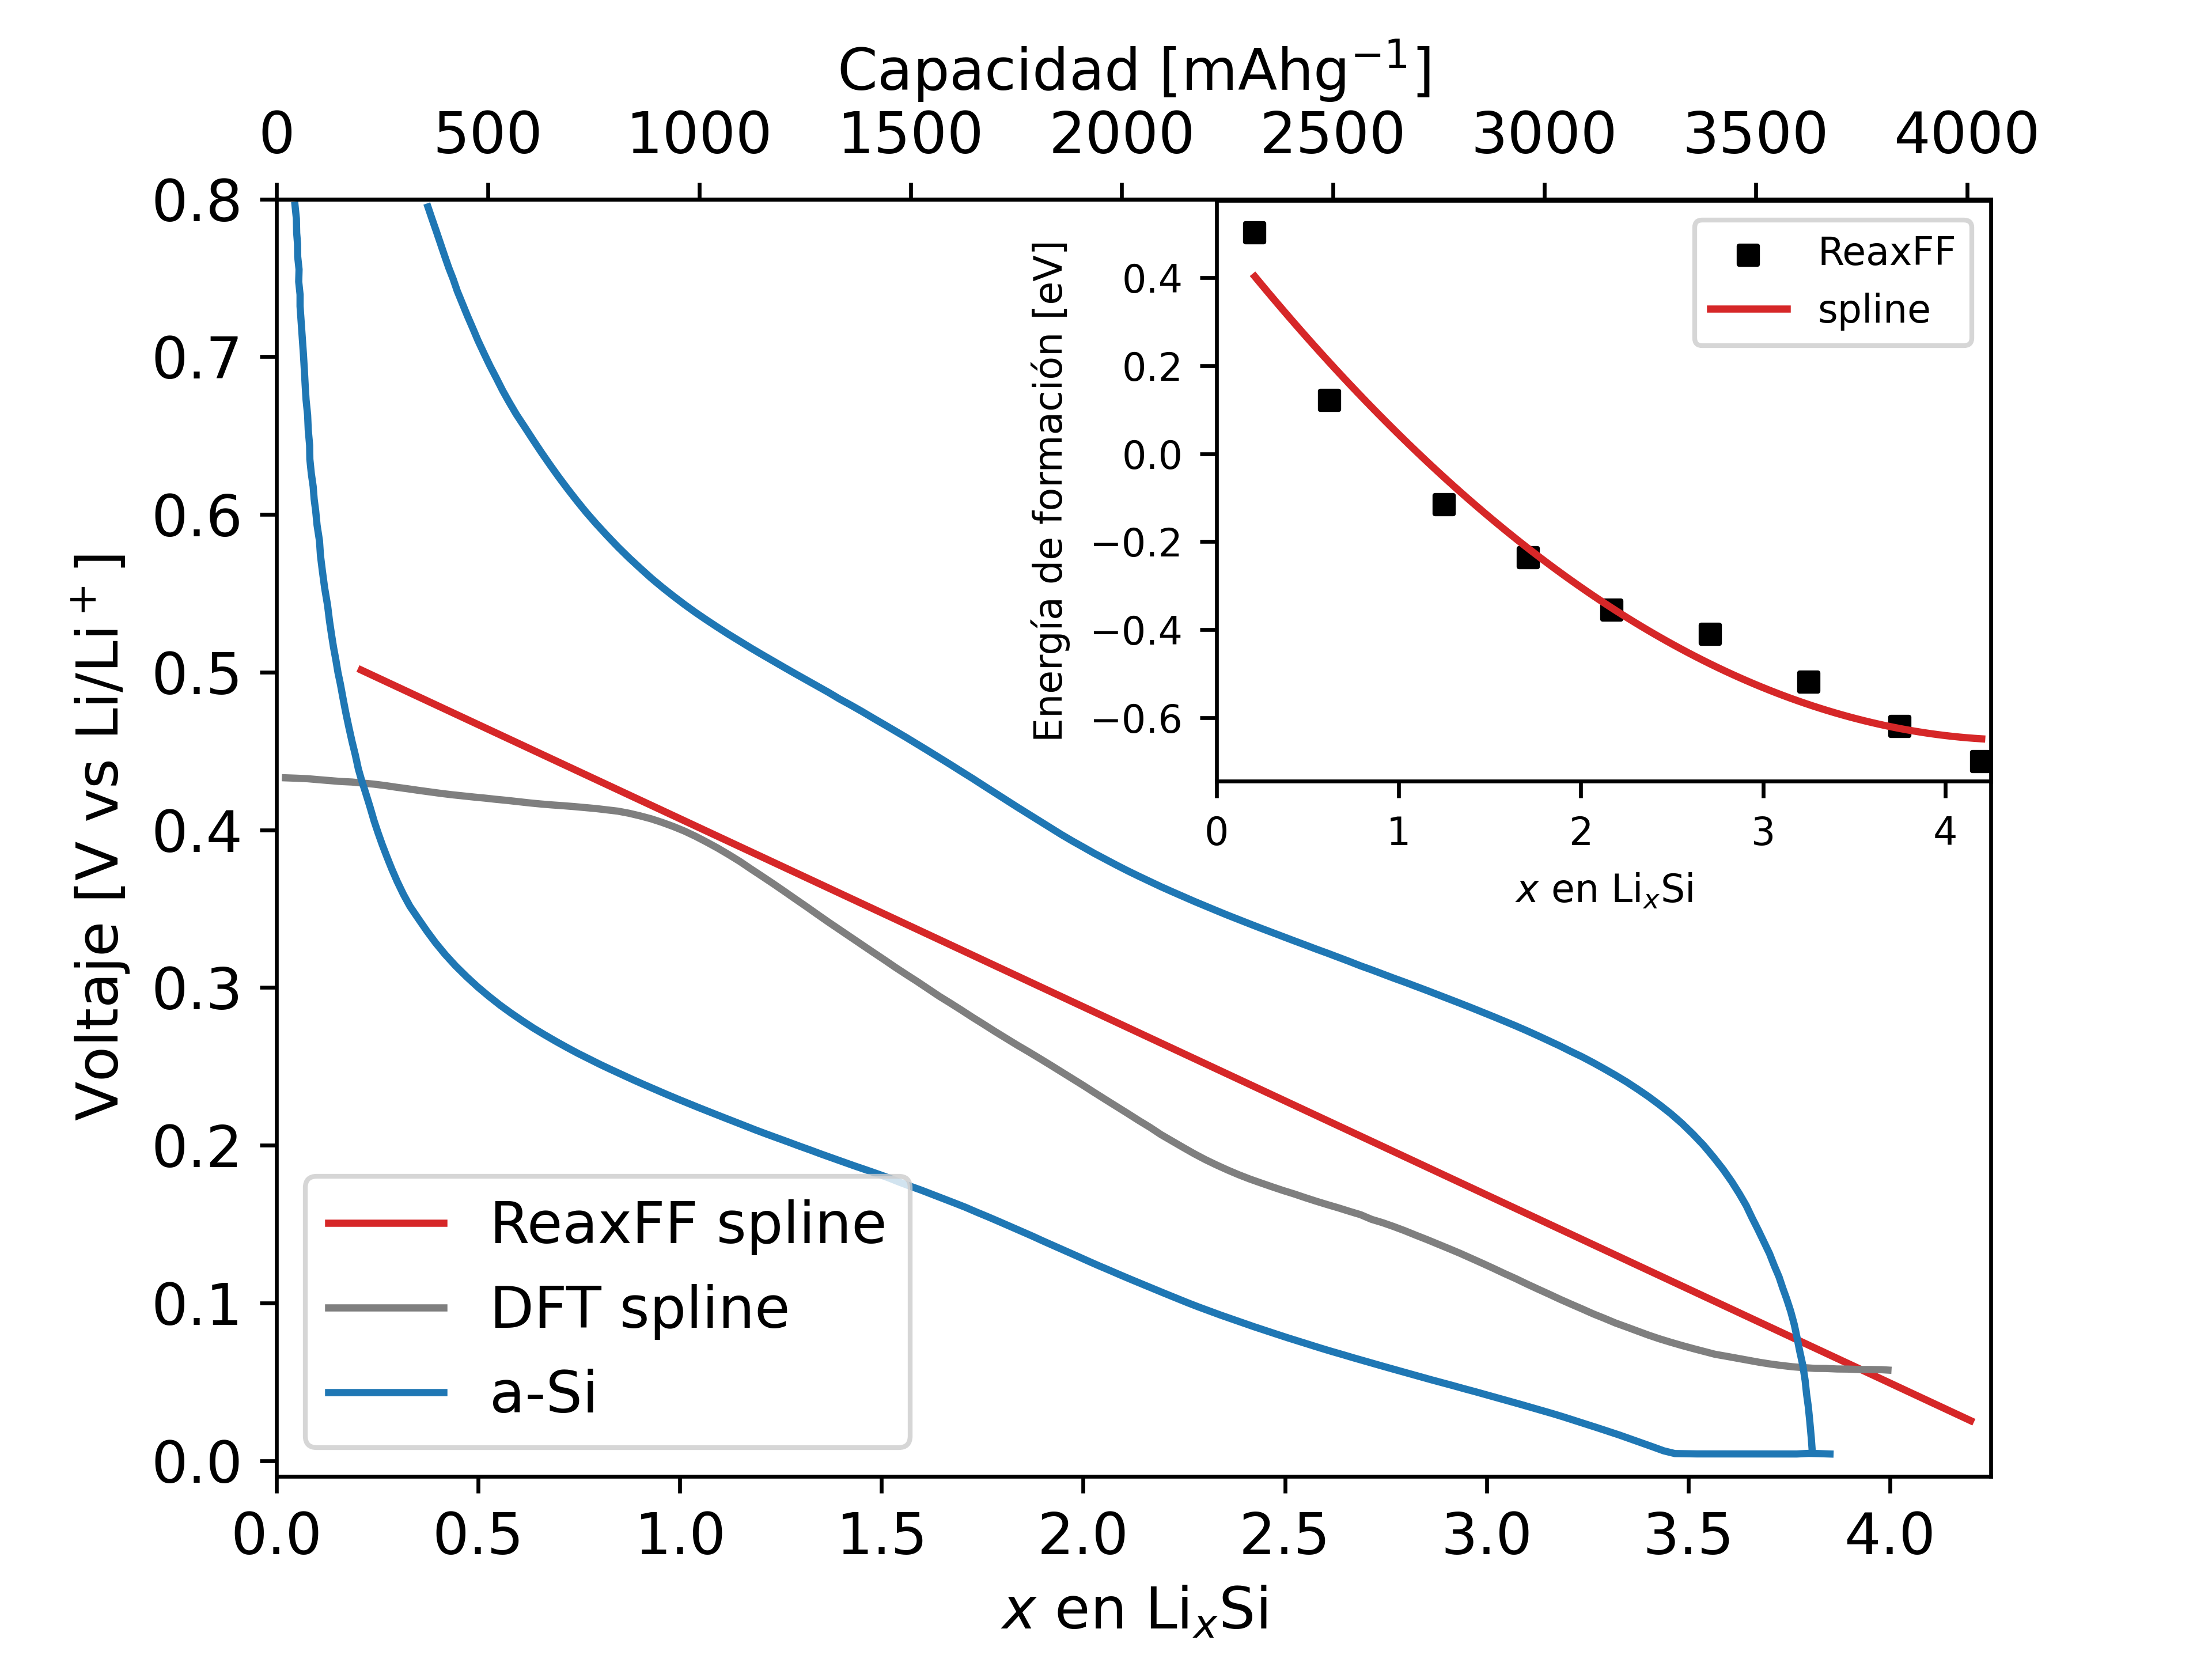
\includegraphics[width=0.8\textwidth]{Silicio/caracterizacion/resultados/electroquimica/voltaje.png}
    \caption{Curvas potencial-concentración para la litiación de ánodos de Si.
    La línea negra corresponde a cálculos de DFT, las líneas azules a 
    curvas medidas experimentalmente en la litiación de Si amorfo y la línea 
    roja es la derivada del \textit{spline} ajustado a los datos de la energía 
    de formación obtenidos con el ReaxFF, presentados en el recuadro.}
    \label{fig:voltaje}
\end{figure}


\subsection{Amorfización del silicio mediante un templado simulado y análisis de la función de distribución radial (RDF)}\label{s:rdfb}

Por último, las mayores discrepancias entre las energías de formación calculadas con DFTB
con respecto a DFT se corresponden a estructuras de silicio amorfo, por lo cual,
se realizó una evaluación extra para este caso. En la Figura \ref{fig:rdfb} se 
muestran las RDFs Si-Si (ver ecuación \ref{eq:rdf}) obtenidas por un templado simulado para cada una de las
parametrizaciones. Además, se compara con el potencial previo de ReaxFF 
\cite{fan2013} y con una determinación experimental \cite{laaziri1999}. Para 
obtener las estructuras amorfas se comenzó con una celda de c-Si con 64 átomos 
a la cual se le realizó un templado simulado en el ensamble $NVT$ utilizando el 
termostato de Nosé-Hoover. El mismo consistió en una etapa inicial de 
calentamiento lineal desde temperatura ambiente hasta 3000 K durante 100 ps, luego una
termalización a dicha temperatura por 600 ps y, por último, un enfriamiento 
exponencial de 600 ps hasta llegar a temperatura ambiente. Para todas las etapas
se utilizó un paso temporal de 1 fs. Para el cómputo de las RDFs que se muestran
en la Figura \ref{fig:rdfb} se equilibró la estructura alcanzada a temperatura 
ambiente durante 100 ps. Puede destacarse que los resultados del conjunto B de parámetros muestran
una concordancia excelente con los datos experimentales de la referencia 
\cite{laaziri1999}, lo que convierte a esta parametrización en la más adecuada
para simulaciones futuras. Los archivos de dichos parámetros están disponibles
en un repositorio público \cite{dftb_lisi}.
\begin{figure}[h!]
    \centering
    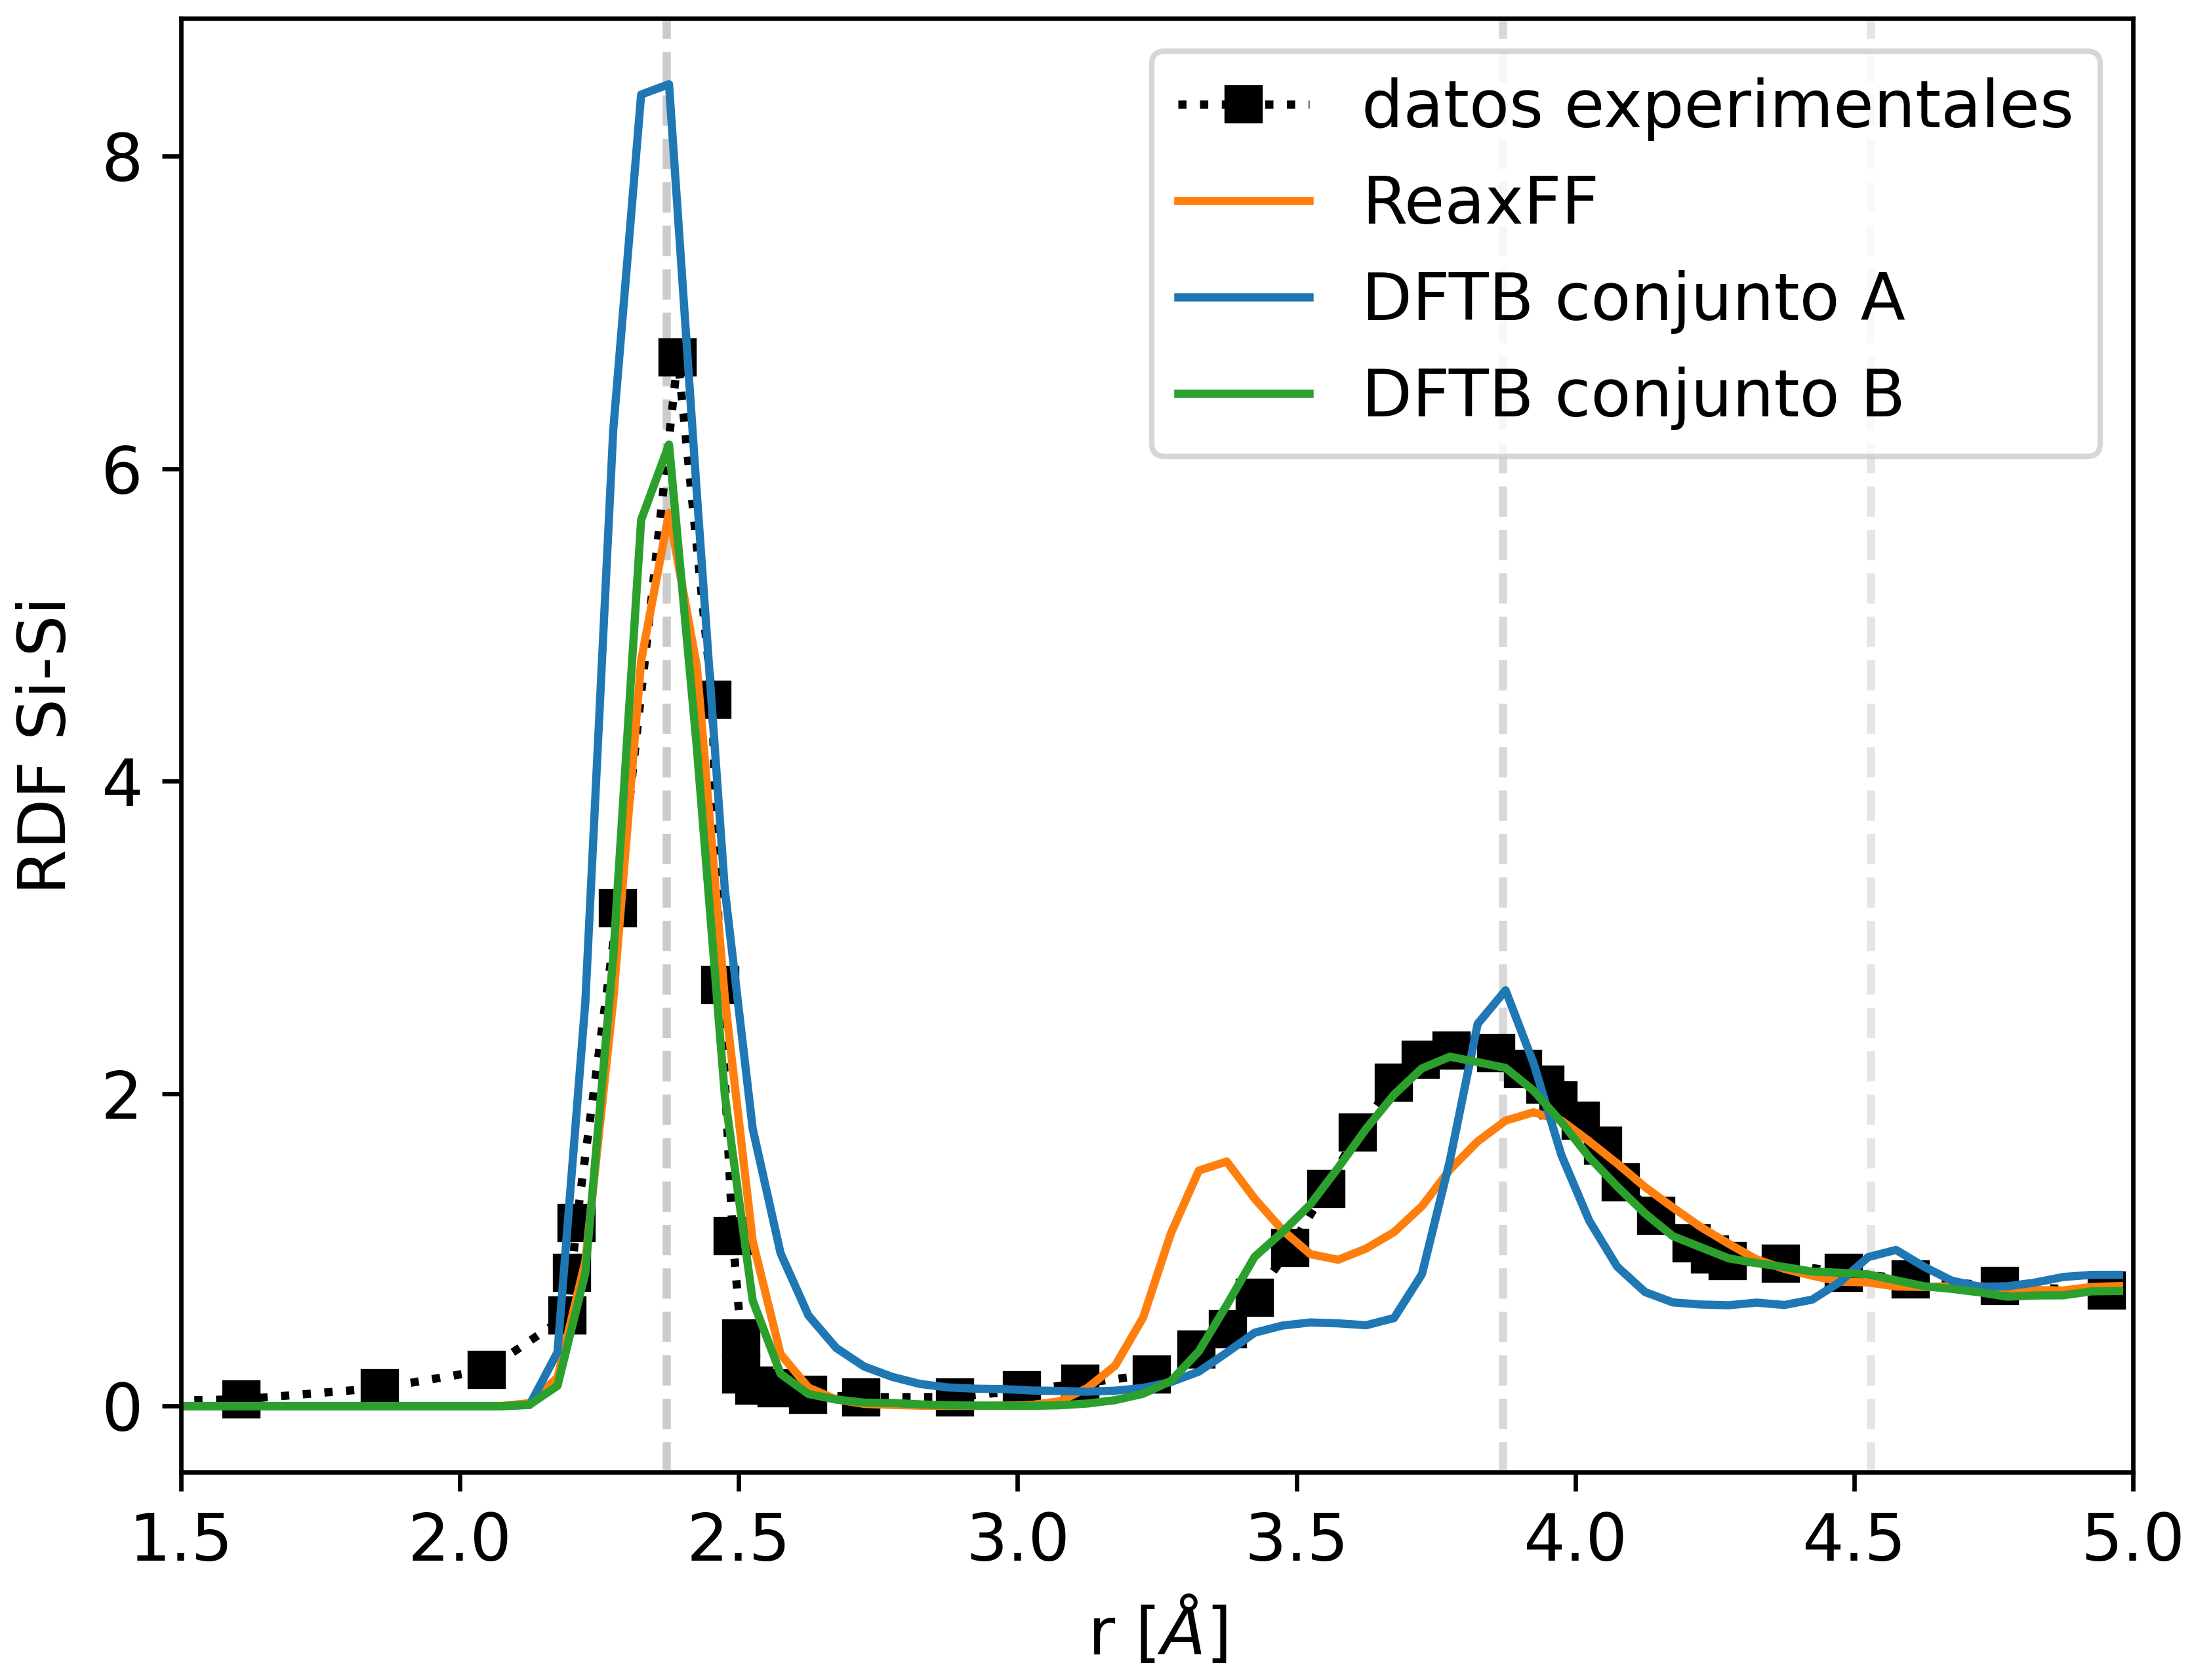
\includegraphics[width=.7\textwidth]{Silicio/modelo/resultados/rdf/rdf.png}
    \caption{Función de distribución radial (RDF) de silicio amorfo para los
    conjuntos A y B de parametrizaciones. Los resultados se comparan con 
    mediciones de la referencia \cite{laaziri1999} y con los resultados obtenidos
    utilizando el ReaxFF \cite{fan2013}. Las líneas grises discontinuas verticales
    muestran dónde estarían los picos del silicio cristalino a 0 K. Se encuentra 
    una concordancia excelente entre el experimento y la parametrización del 
    conjunto B.}
    \label{fig:rdfb}
\end{figure}


% Copyright (c) 2024, Francisco Fernandez
% License: CC BY-SA 4.0
%   https://github.com/fernandezfran/thesis/blob/main/LICENSE
\subsection{Número de coordinación}

De la misma manera que se utilizaron las distribuciones radiales parciales, se pueden
obtener los números de coordinación para un dado tipo de átomo utilizando la ecuación
\ref{eq:cn} definida en la sección \ref{ss:cn} con la $g(r)$ correspondiente. Debido
a que en los materiales amorfos la primera y la segunda esfera de coordinación pueden 
llegar a estar superpuestas, el límite superior de integración no está definido 
unívocamente para todas las concentraciones consideradas \cite{lamparter1995}.
El número de coordinación promedio para átomos de Si vecinos de otros átomos 
de Si se calculó utilizando un radio de 
corte de 3 \AA. Lo mismo se realizó para Li-Li definiendo un radio de corte de 
4 \AA. Para el caso de Si-Li se utilizó el criterio de considerar como radio de 
corte el valor $r$ para el cual la $g(r)$ presenta un mínimo entre los dos picos
a primeros y segundo vecinos. Los resultados se muestran en la Figura 
\ref{fig:cn}a.
\begin{figure}[h!]
    \centering
    \includegraphics[width=\textwidth]{Silicio/caracterizacion/resultados/cn/cn.png}
    \caption{Número de coordinación en función de la concentración de litio para
    Li-Li, Si-Si y Si-Li. Como radios de corte se utilizaron las distancias 
    del pico de la RDF correspondiente. En los casos en que no se aprecia la barra
    de error, la misma es menor que el tamaño de los puntos. (a) Primero número 
    de coordinación. (b) Segundo número de coordinación.}
    \label{fig:cn}
\end{figure}

Para el caso del CN$_{\text{Si}-\text{Si}}$, se tiene que esta cantidad decrece de 4 a 2, a 
medida que la concentración de Li aumenta. Esto indica que a valores pequeños de 
$x$ la estructura de Si mantiene sus conexiones tetraédricas, mientras que para
valores grandes de $x$ el Si tiende a formar cadenas periódicas unidimensionales.
En la red de silicio amorfa, analizada con más detalle en la sección 
\ref{s:clusters}, se presenta una estructura 3d-periódica para valores bajos de 
$x$, donde el CN se encuentra alrededor de 4. Luego, se alcanza una estructura 1d-periódica 
para valores grandes de $x$, donde los enlaces Si-Si tienden a formar 
cadenas, que pueden verse para $x = 3.75$ donde se tiene CN = 2.05, por ejemplo.
El CN de Si-Li y Li-Li presenta valores pequeños para concentraciones 
bajas y aumenta monótonamente hasta alcanzar valores de 10 y 12, respectivamente, 
que se asemejan al valor de una estructura de empaquetamiento compacto.

Los resultados para el segundo número de coordinación se presentan en la Figura 
\ref{fig:cn}b. Estos resultados se obtuvieron considerando un cascarón con un 
radio de corte interno y otro externo, elegidos de manera tal que incluyan el 
segundo pico de la RDF. La elección de dichos valores varió dependiendo del tipo
de átomos que se consideraron. En todos ellos se tomó como radio de corte interno 
el radio de corte del primero número de coordinación. Luego, para el radio de 
corte externo se utilizaron valores de 5.0 \AA\ para Si-Si y 6.0 \AA\ para Li-Li
y Si-Li.

Para los valores de CN$_{\text{Si}-\text{Si}}$ se observa un aumento para concentraciones bajas
de Li, si se lo compara con el CN de primeros vecinos. Para valores mayores de $x$,
se puede ver cómo el valor de CN también tiende a 2, lo cual es coherente con la
formación de cadenas que se notó previamente. La tendencia cualitativa del segundo
CN para Li-Li y Si-Li es la misma que la observada en el primer CN, sólo que ahora
empieza en un valor cercano a 5 y tiende a 35 y 40, respectivamente. Este valor 
es mucho mayor que el que se tiene para los segundos vecinos en una estructura 
de empaquetamiento compacto, que es 6 para la estructura cristalina FCC. Incluso 
es mayor a la suma del segundo (6) y del tercer vecino (24) esperado para la red 
FCC.


% Copyright (c) 2024, Francisco Fernandez
% License: CC BY-SA 4.0
%   https://github.com/fernandezfran/thesis/blob/main/LICENSE
\subsection{Formación de conglomerados (clusters)}\label{s:clusters}

Analizando la formación de \change{conglomerados} (clusters) por medio del algoritmo DBSCAN 
\cite{ester1996}, en el cual puede definirse un radio de corte para el cual se 
deja de considerar que los átomos están enlazados entre sí (es decir, formando 
clusters), se encuentra que las estructuras amorfas de silicio no pueden ser 
clasificadas en diferentes tipos de clusters, las mismas reflejan más bien 
una red amorfa. Esto viene de interpretar los gráficos que se presentan en la 
Figura \ref{fig:clusters}. 
\begin{figure}[h!]
    \centering
    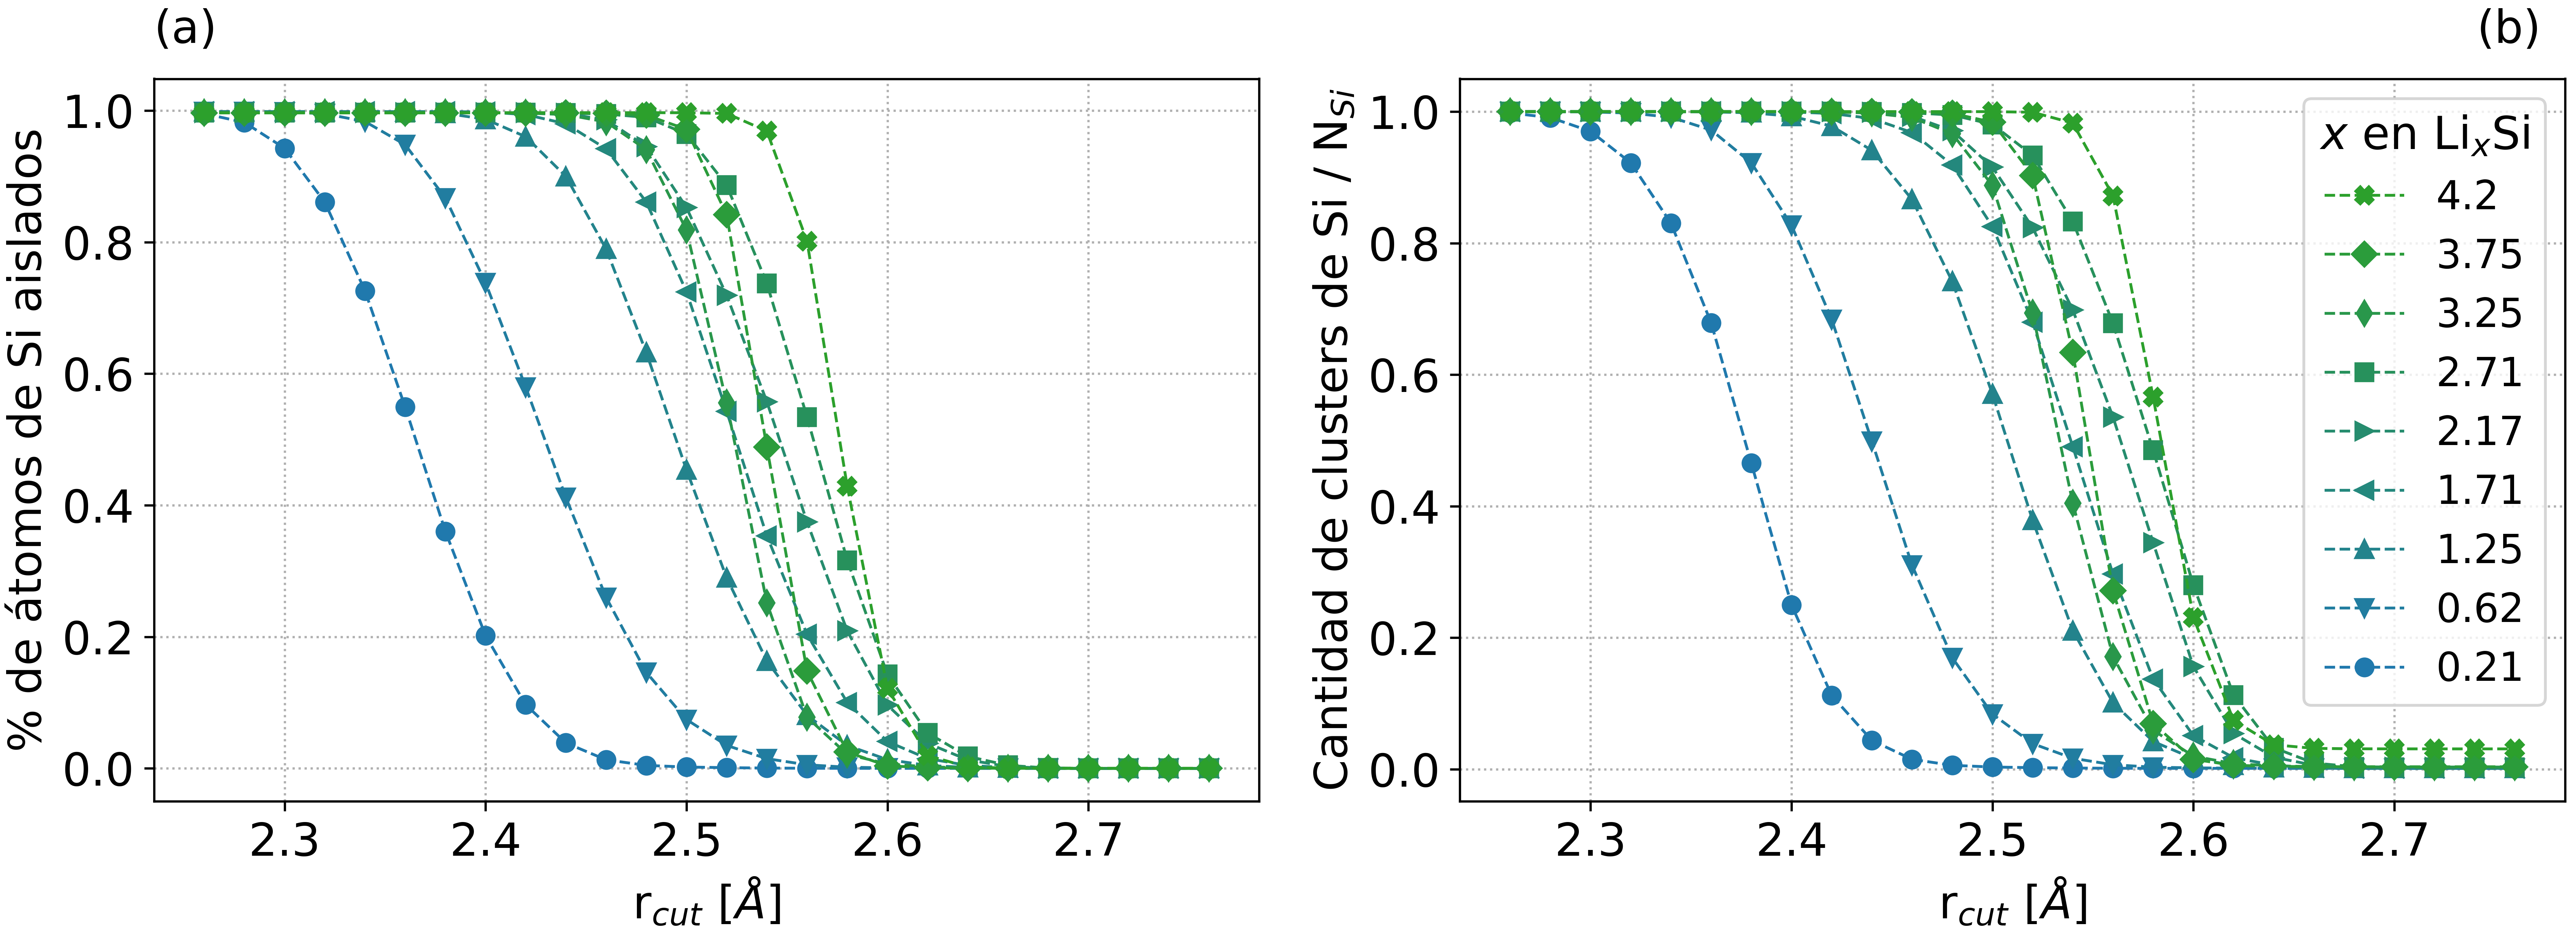
\includegraphics[width=\textwidth]{Silicio/caracterizacion/resultados/clusters/clusters.png}
    \caption{Formación de clusters indicando una red amorfa de silicio. (a) 
    Fracción de átomos de Si aislados en función de la elección del
    radio de corte. (b) Número de clusters de Si sobre el número total de átomos 
    de Si.}
    \label{fig:clusters}
\end{figure}

En particular, en la Figura \ref{fig:clusters}a se define la fracción 
de átomos de Si que están a una distancia mayor que $r_{cut}$ de otros átomos de 
Si. Cuando el radio de corte es mayor que la distancia a la cual termina el 
primer pico de la RDF$_{\text{Si}-\text{Si}}$, no se tienen átomos de Si que cumplan esta 
propiedad, es decir, no hay átomos de Si que se encuentren aislados en el sistema,
incluso a concentraciones altas de Li. Esto refleja que el a-Si se comporta como 
una red en la cual todos los átomos de silicio están interconectados entre sí, 
cosa que también se puede deducir de la Figura \ref{fig:clusters}b, en la cual 
se tiene que cuando el radio de corte es menor que el primer pico de la RDF$_{\text{Si}-\text{Si}}$ 
el número de clusters es igual al número de átomos de Si, pero que cuando este 
radio es más grande que la distancia a la cual termina el primer pico, hay un 
solo cluster.


\subsection{Interconexión de clusters}\label{s:interconexion}

Para determinar qué es lo que genera una estructura compleja en el segundo pico de la 
RDF$_{\text{Si}-\text{Li}}$, ver Figura \ref{fig:rdf}, se realizó un análisis similar al reportado por Ding \textit{et al.}
\cite{ding2015}. Estos autores analizaron la correlación en la distancia de a
pares de los segundos vecinos más cercanos en términos de las conexiones entre
clusters, definiendo un poliedro de coordinación alrededor del átomo central 
considerado para la RDF y sus segundos vecinos. El número de átomos compartidos
entre estos dos poliedros de coordinación enlazados fueron utilizados para 
establecer categorías y analizar sus contribuciones a la RDF. Estas categorías
dependen del hecho de que los poliedros comparten un vértice (1 átomo), una 
arista (2 átomos), una cara de los poliedros (3 átomos) o cuadriláteros 
distorsionados o tetraedros aplastados (4 átomos). De una forma similar al trabajo de Ding, se deconvolucionó el segundo pico de la RDF calculando la RDF parcial 
de distintas categorías, donde cada categoría se define por el número de átomos de
Li que interconectan un átomo de Si con su segundo vecino de Li. El comportamiento
detallado se presenta en la Figura \ref{fig:interconexiones}. Puede afirmarse a 
grandes rasgos que para concentraciones bajas de Li en las aleaciones, hay una 
predominancia de segundos vecinos de Li que tienen una o ninguna interconexión 
con los vecinos de Li de la primera esfera de coordinación Si-Li. Para $x > 1.0$
la contribución del segundo vecino de Li interconectado con dos o más átomos de 
Li de la primera esfera de coordinación Si-Li comienza a ser predominante y la
contribución de los átomos de Li sin conectarse empieza a decaer. Para $x > 3.0$,
la contribución del primer pico del segundo vecino de Li interconectado dos o
tres veces se vuelve relevante mientras que aparecen contribuciones de cuatro o
más interconexiones.
\begin{figure}[h!]
    \centering
    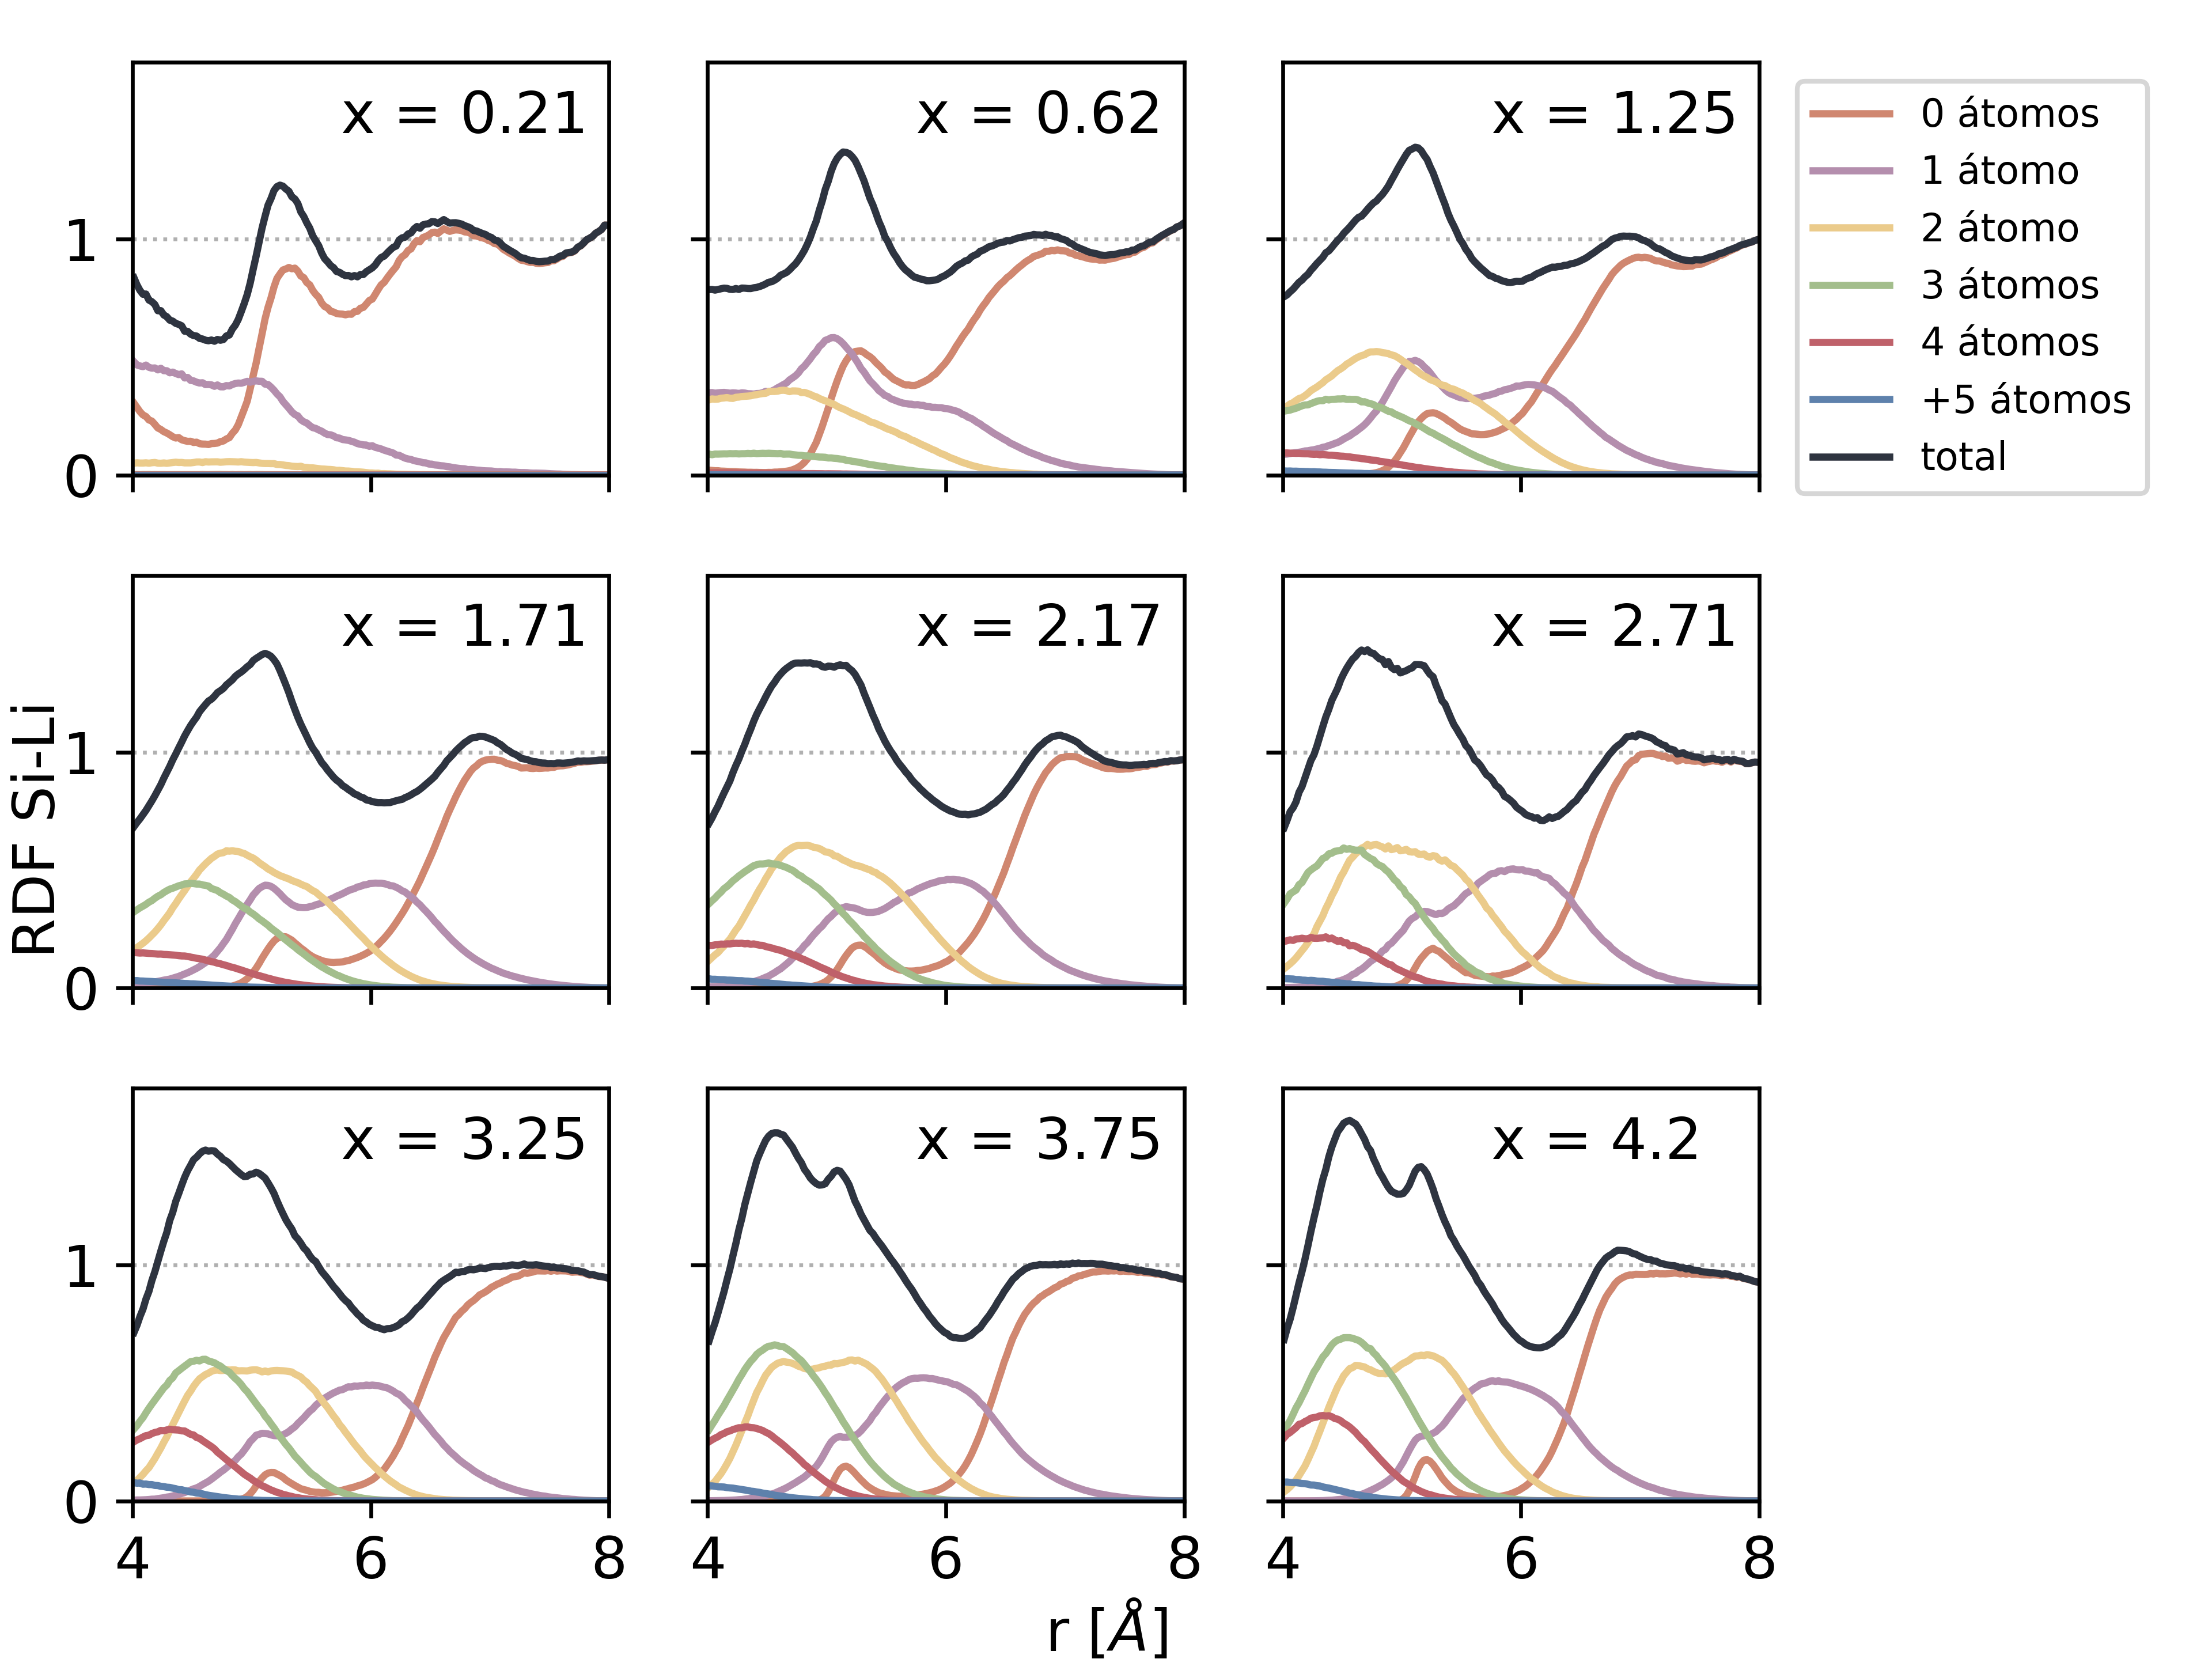
\includegraphics[width=\textwidth]{Silicio/caracterizacion/resultados/interconexion/interconexiones.png}
    \caption{Interconexiones de los segundos vecinos más cercanos de Li con un 
    átomo central de Si para cada valor de $x$ en Li$_x$Si considerado \cite{ding2015}. El número 
    de primeros vecinos más cercanos que conectan a los segundos vecinos más 
    cercanos con el átomo central de Si se indica en el recuadro de las figuras. 
    Además de la RDF$_{\text{Si}-\text{Li}}$ total, se grafica cada una de las contribuciones 
    de los diferentes tipos de interconexiones posibles.}
    \label{fig:interconexiones}
\end{figure}

Mientras que el comportamiento presentado en la Figura \ref{fig:interconexiones}
es más bien complejo, pueden establecerse tendencias generales que ayudan a 
entender mejor que es lo que sucede. Si se divide la RDF$_{\text{Si}-\text{Li}}$ en dos 
contribuciones de segundos vecinos, la primera de ellas, que se encuentra a una
distancia entre 4.0 \AA\ y 5.0 \AA, se puede atribuir a los átomos que tienen dos 
o más interconexiones de Li, mientras que la segunda de ellas, entre 5.0 \AA\ y
5.6 \AA, se corresponde con los átomos que tiene una o ninguna interconexión de 
Li. Utilizando esta clasificación, se muestra en la Figura 
\ref{fig:interconexiones-areas} la fracción del área que representa cada una de
estas categorías en función de la concentración de litio.
\begin{figure}[h!]
    \centering
    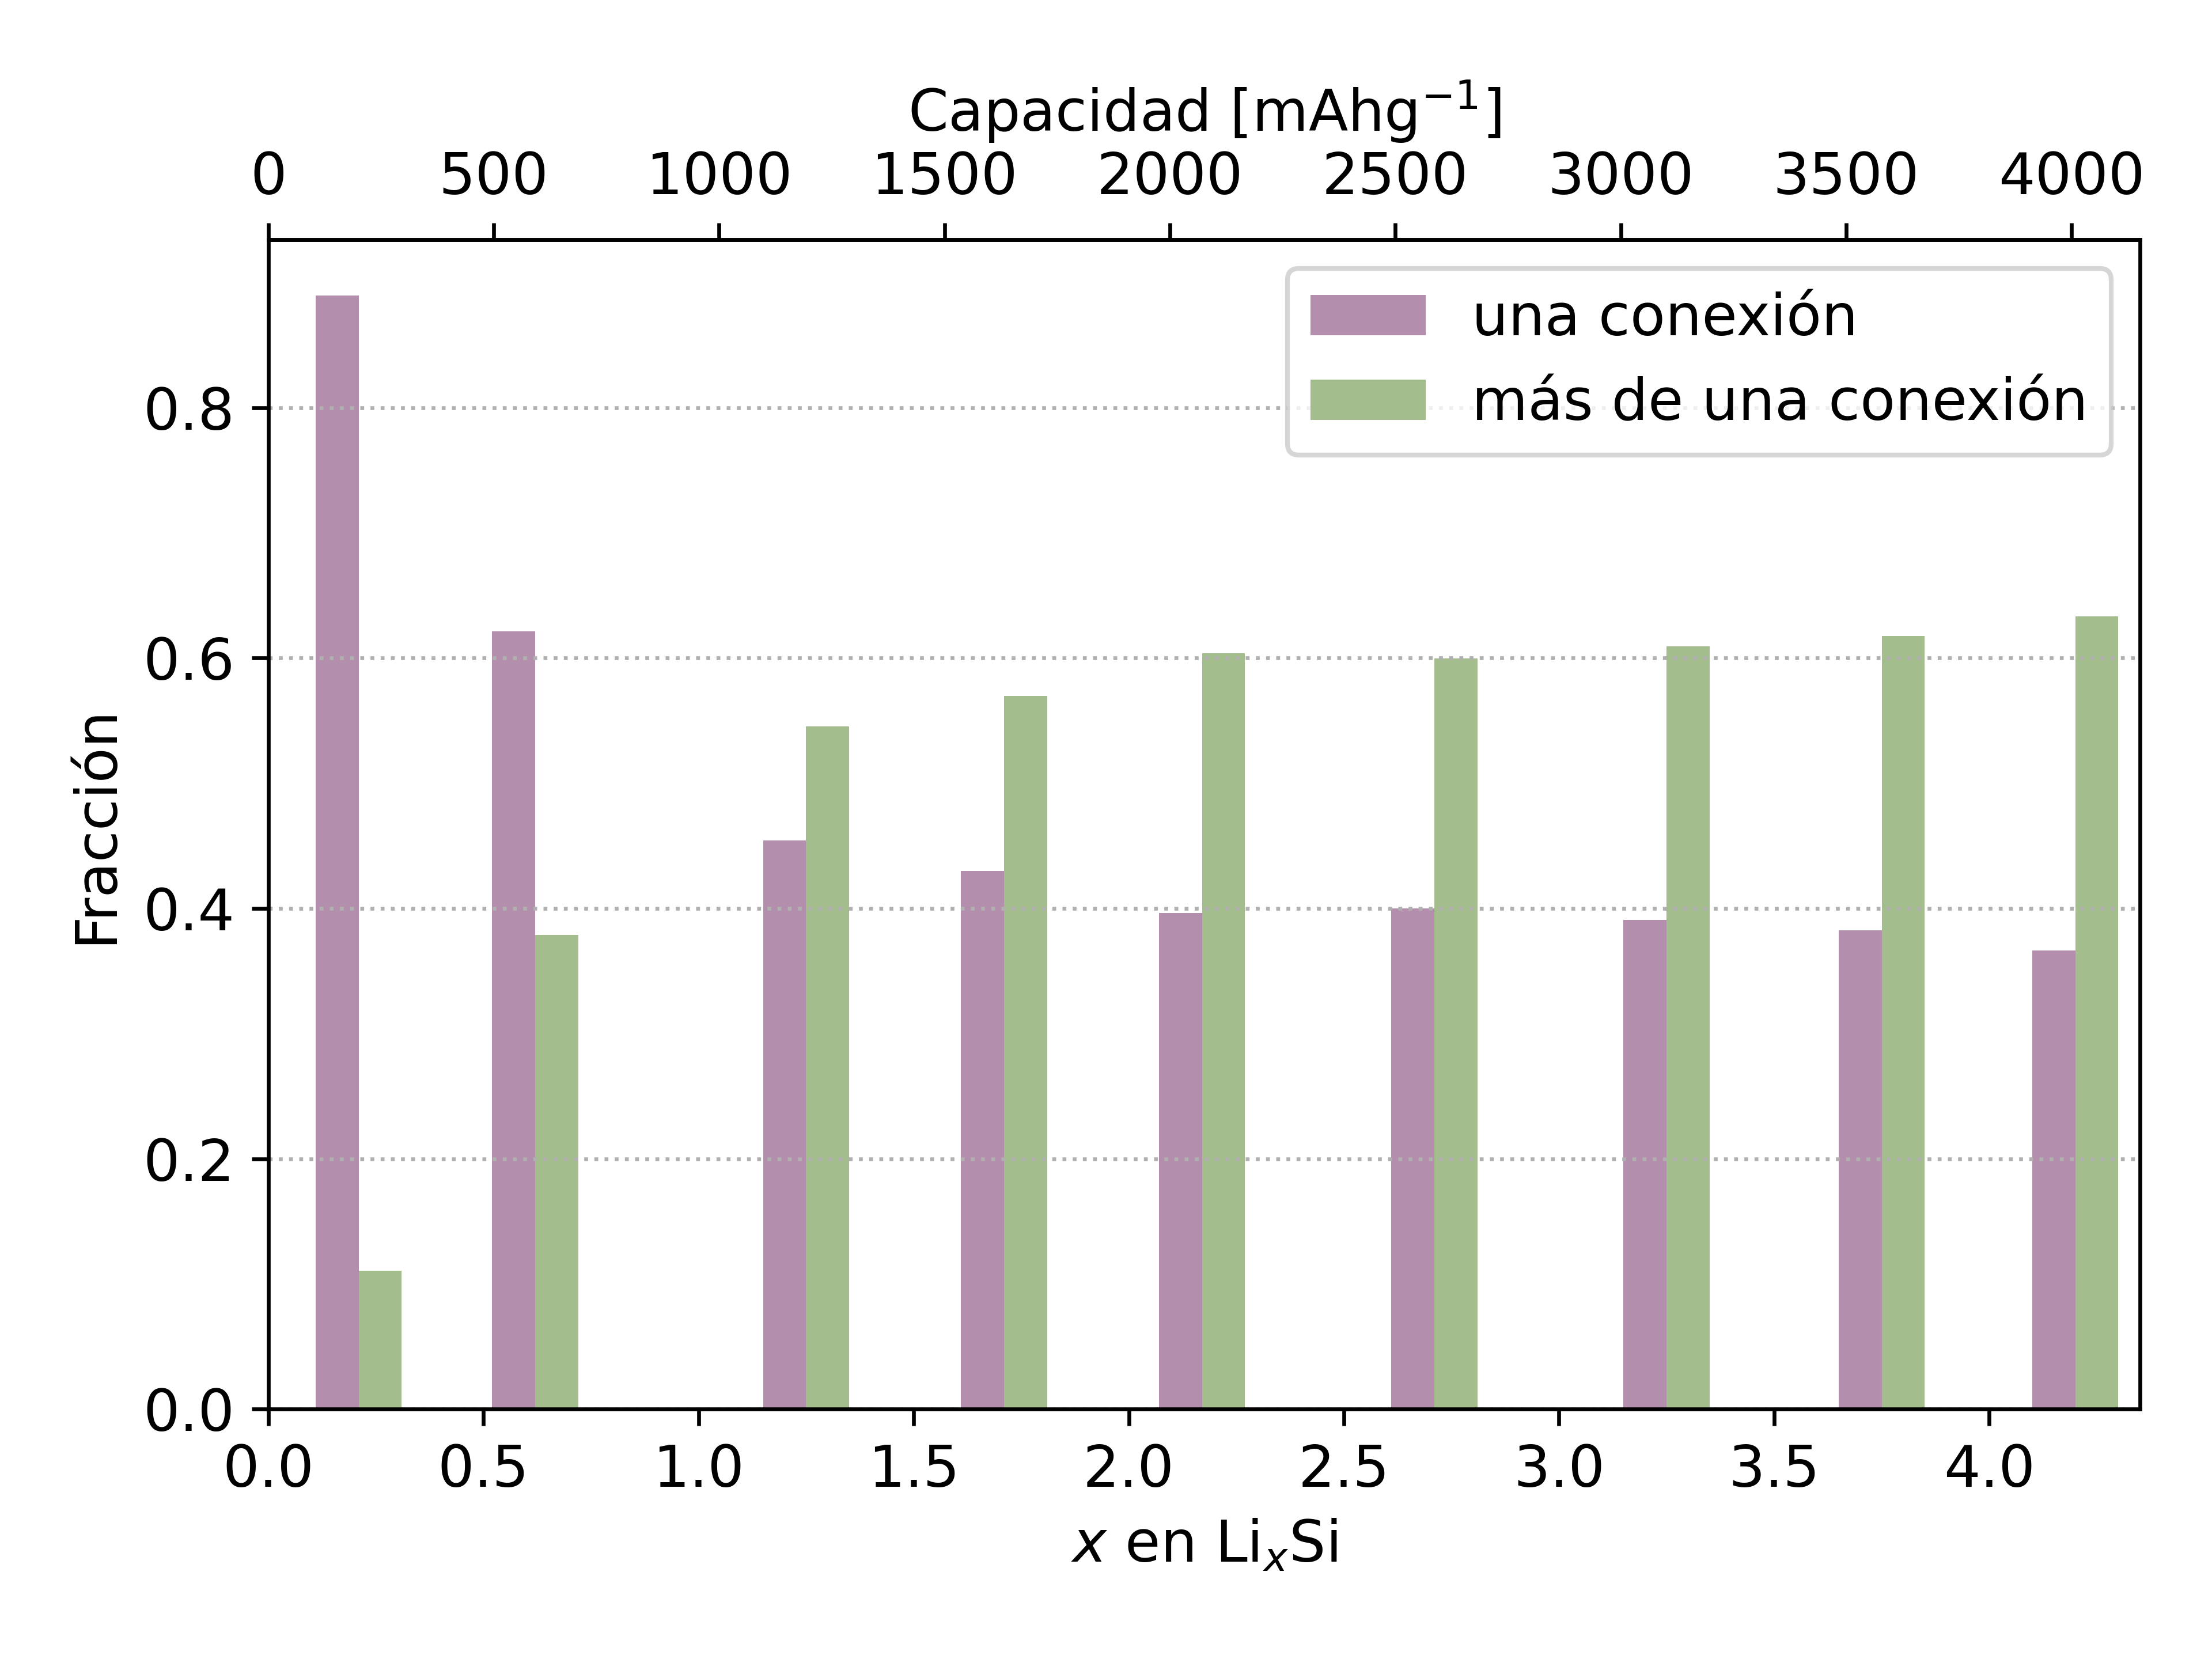
\includegraphics[width=0.7\textwidth]{Silicio/caracterizacion/resultados/interconexion/interconexiones-areas.png}
    \caption{Evolución con la concentración de la fracción que representa cada
    categoría de interconexiones de Li al área total del segundo pico de la 
    RDF$_{Si-Li}$.}
    \label{fig:interconexiones-areas}
\end{figure}


\subsection{Orden de corto alcance}

El término orden de corto alcance (SRO, de sus siglas en inglés 
\textit{short-range order}) se utiliza para denotar el ordenamiento de los átomos
que rodean a uno específico en una cáscara. Del mismo modo, el término 
\textit{clustering} se ha definido como la tendencia de los átomos similares a 
estar cerca unos de otros. Ambos conceptos se refieren a un orden estructural 
entre átomos vecinos, pero no son necesariamente persistentes a distancias más 
largas. Warren ~\cite{warren69} y Cowley ~\cite{cowley1950} definieron un 
parámetro (WCP) para caracterizar estos tipos de ordenamientos de la siguiente 
manera:
\begin{equation}
    WCP = 1 - \frac{p_{A-B}}{m_B} = 1 - \frac{p_{B-A}}{m_A},
\end{equation}
donde $p_{A-B}(p_{B-A})$ es la probabilidad de tener un átomo de tipo B(A) como
vecino de un átomo de tipo A(B) y $m_B(m_A)$ es la concentración global de átomos
B(A), expresadas en fracciones molares. La igualdad, en ambas definiciones 
posibles del WCP, viene del hecho de que la probabilidad de encontrar a un átomo 
de tipo A como vecino de un átomo de tipo B es igual a la de tener un átomo de 
tipo B como vecino de un átomo de tipo A, esto es $m_A p_{A-B} = m_B p_{B-A}$.

Los valores que se obtienen de utilizar el parámetro WCP en sistemas del tipo
A$_x$B indica una aleatoriedad completa si es igual a cero, preferencia por 
átomos de distinto tipo si $WCP < 0$ y preferencia por átomos del mismo tipo si 
$WCP > 0$. Aunque este parámetro permite un análisis cuantitativo notable, sólo
se define para sistemas cristalinos en los que cada átomo tiene el mismo número
de vecinos. ~\cite{warren69}

A continuación se extiende esta idea para definir un nuevo parámetro, 
$\theta_{A-B}$, que es adecuado para caracterizar estructuras amorfas, de la 
siguiente manera:
\begin{equation}
    \theta_{A-B} = \ln \left( \frac{C_{A-B}}{C_{Bulk}} \right),
\end{equation}
donde A indica la naturaleza del átomo que se considera como central y B el tipo
de átomo que se considera como vecino, equivalente a la definición de WCP. En
este caso, la relación entre la concentración local y la concentración global se 
calcula a partir de la integración de la distribución radial de a pares parcial,
$g_{A-B}(r)$, en una esfera al rededor del átomo central,
\begin{equation}
    \frac{C_{A-B}}{C_{Bulk}} = \frac{1}{V(r_{cut})} \int_0^{r_{cut}} g_{A-B}(r) dV,
\end{equation}
donde $r_{cut}$ y $V(r_{cut})$ son el radio de corte y el volumen de la esfera 
considerada. Ya que en $g_{A-B}(r)$ no hay dependencia angular, $dV$ puede 
escribirse como $4 \pi r^2 dr$. Esta cantidad puede pensarse como la 
concentración promedio dentro de la esfera relativa a la del material 
masivo. Así, de forma análoga al parámetro de WCP, $\theta_{A-B}$ indica 
la tendencia SRO o el \textit{clustering} para cualquier tipo de átomo dado.
Si $\theta$ es positivo, indica una acumulación de átomos relativa al 
\textit{bulk}, mientras que si es negativo indica una disminución. Si es igual a 
cero se tiene una aleatoriedad completa. Este nuevo parámetro también satisface 
la relación $\theta_{A-B} = \theta_{B-A}$ de la misma manera que se discutió para
el parámetro de WCP, ya que por definición $g_{A-B}(r) = g_{B-A}(r)$. Por lo cual 
se tiene que el parámetro $\theta_{A-B}$ da información similar a la que provee 
el WCP, pero además es aplicable a sistemas amorfos.

La figura \ref{fig:sro} muestra la variación del parámetro $\theta$ en función 
de la concentración de Li. Hay tres posibilidades para el análisis de $\theta$ en
sistemas de Li$_x$Si ($\theta_{Li-Li}$, $\theta_{Si-Si}$ y $\theta_{Si-Li}$), ya
que $\theta_{Si-Li} = \theta_{Li-Si}$. Para todos los casos se consideraron los
mismos radios de corte que en los cálculos del número de coordinación, luego del
primer pico de la RDF correspondiente.
\begin{figure}[th]
    \centering
    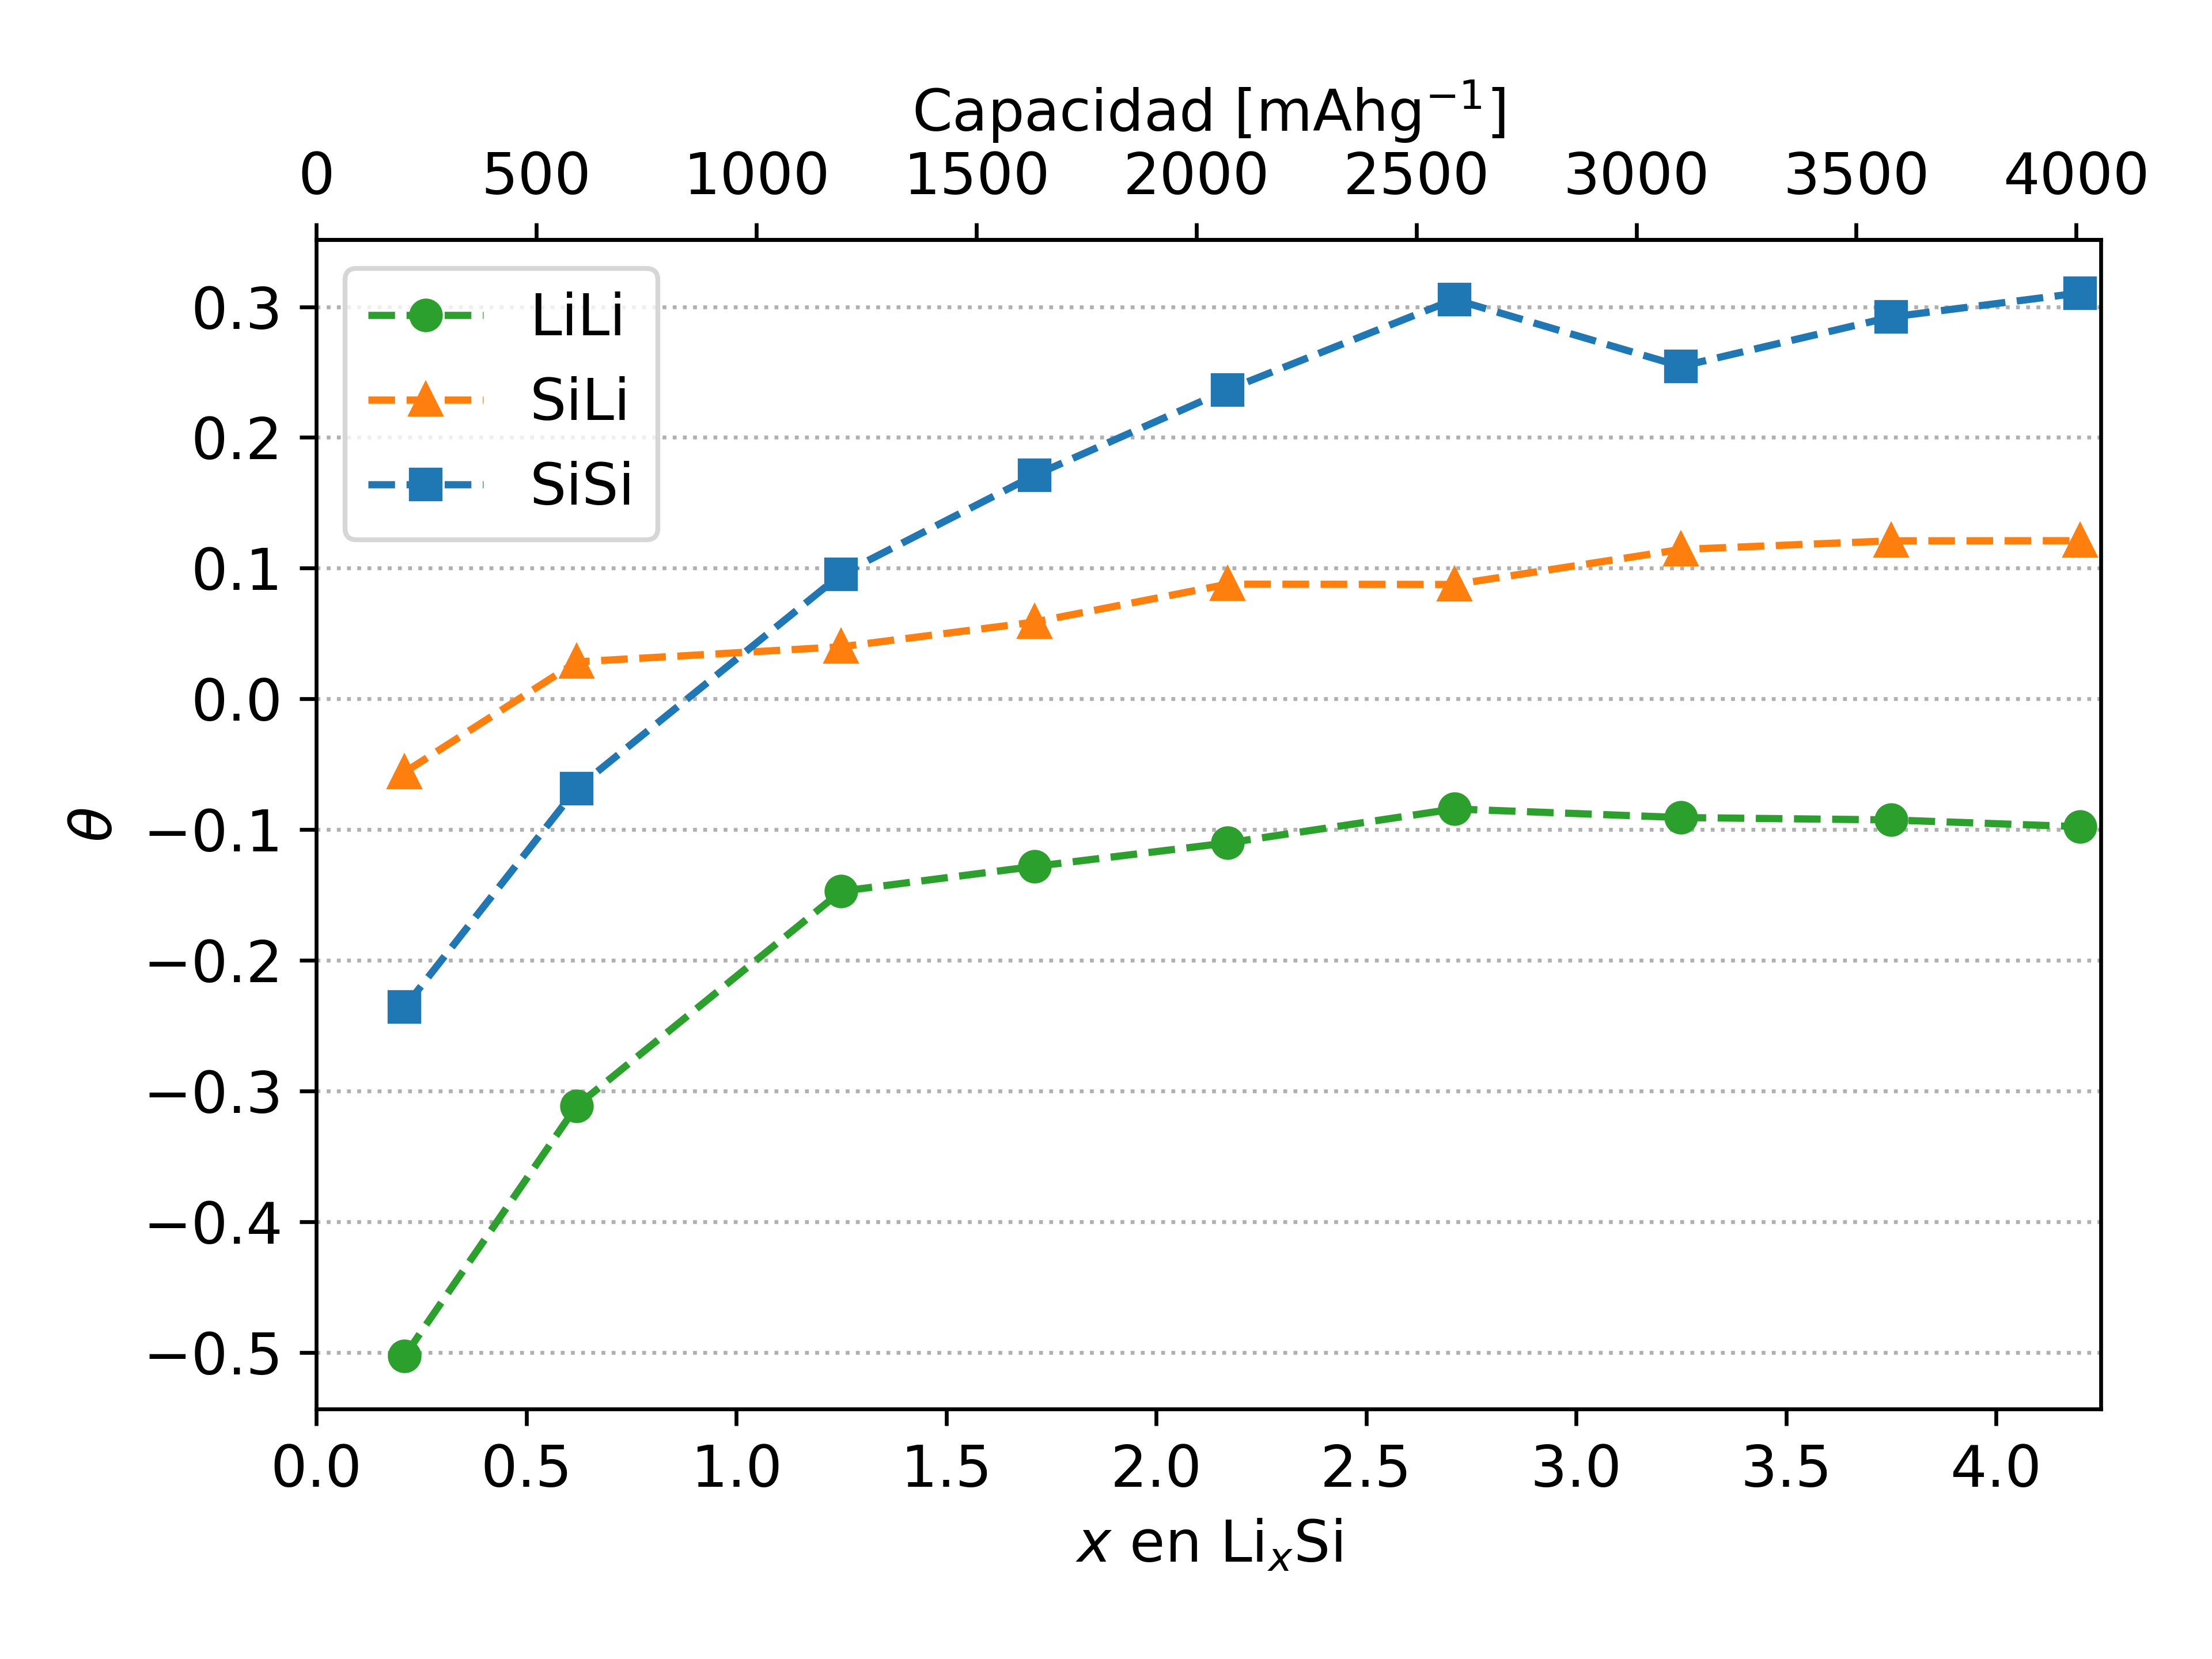
\includegraphics[width=0.8\textwidth]{Silicio/caracterizacion/resultados/sro/sro.png}
    \caption{Parámetros $\theta_{Li-Li}$, $\theta_{Si-Li}$ y $\theta_{Si-Si}$ 
    en función de la concentración de Li. El primer subíndice indica el tipo de
    átomo que se considera como central mientras que el segundo es el vecino. El
    radio de corte se eligió luego del primer pico de la RDF correspondiente.}
    \label{fig:sro}
\end{figure}

Como tendencia general, puede notarse que todos los valores de $\theta$ aumentan
cuando crece la cantidad de litio en el sistema, $x$, y que se estabiliza para 
valores grandes de $x$. Este comportamiento monótono y la disminución en la 
pendiente para concentraciones altas está correlacionado con el comportamiento
presentado en el análisis de los números de coordinación.

En el caso de $\theta_{Si-Si}$, alcanza un valor positivo aproximadamente 
constante para $x > 2.5$, mostrando una correlación fuerte con la presencia de 
cadenas lineales de Si, previamente discutidas y observadas en la figura 
\ref{fig:amorfas}. Aunque la presencia de estas cadenas se puede inferir a partir
de los valores de los CN en $x$ altos, $\theta$ es más sensible al SRO, ya que
está normalizado por la concentración global. Esta propiedad de $\theta$ permite
un análisis más claro incluso si las cadenas están interactuando entre sí, como
es el caso para concentraciones bajas de litio.

$\theta_{Si-Li}$ presenta variaciones pequeñas y un valor positivo para todo 
$x > 0.5$, mostrando una acumulación constante de Li al rededor del Si, o, 
análogamente, una acumulación de Si alrededor del Li. Este comportamiento se le 
puede atribuir a la interacción atractiva fuerte en los pares Si-Li. En el caso de 
$\theta_{Li-Li}$, este parámetro es siempre negativo, lo que indica una 
interacción débil Li-Li y la correspondiente disminución de vecinos Li-Li. Por
último, el parámetro $\theta_{Si-Si}$ tiene un valor negativo para $x < 1.0$, 
sugiriendo que la presencia de concentraciones bajas de litio tiende a separar 
los átomos de silicio entre sí. Sin embargo, $\theta_{Si-Si}$ se vuelve positivo
para $x > 1.0$, implicando una acumulación de vecinos de Si sobre átomos de Si, 
relativo a la concentración global. Esto se debe a la formación de estructuras 
Si-Si. Para $x > 2.5$ puede observarse un valor constante de 
$\theta_{Si-Si} \approx 0.3$, revelando la formación de estructuras estables de 
Si-Si dadas por las cadenas previamente mencionadas.


% % Copyright (c) 2024, Francisco Fernandez
% License: CC BY-SA 4.0
%   https://github.com/fernandezfran/thesis/blob/main/LICENSE
\section{Conclusiones del capítulo}

Con el fin de emular las estructuras amorfas encontradas en muchos experimentos 
electroquímicos, en este capítulo se generaron por computadora estructuras desordenadas de 
aleaciones de Li$_x$Si para varios valores de $x$ utilizando un algoritmo de 
dinámica acelerada y un campo de fuerzas reactivo. La exploración acelerada de 
mínimos locales (AELM) permitió la caracterización de una amplia gama de 
estructuras amorfas. El cambio de volumen de las estructuras litiadas en relación 
con el Si está en concordancia con los resultados experimentales de microscopía de fuerza atómica. Las
energías de las estructuras obtenidas representan bien el comportamiento 
electroquímico de la curva de potencial en función de la concentración de Li. Se 
analizó la función de distribución radial de a pares para los diferentes tipos de 
pares atómicos y se dilucidó la estructura compleja del segundo pico del RDF 
Si-Li mediante un análisis de interconexión de clusters. Además, haciendo un 
análisis de la formación de clústeres en función del radio de corte, se demostró 
que las estructuras amorfas no presentan diferentes enlaces de Si ni átomos de Si 
aislados. En su lugar, se encontró que el sistema se comporta como una red amorfa.
Estudiando los números de coordinación de primeros y segundos vecinos para las 
diferentes concentraciones, se mostró que esta red amorfa mantiene las conexiones 
tetraédricas para bajas concentraciones de Li y que tiende a formar cadenas lineales para 
altas concentraciones de Li. Por último, la definición de un nuevo parámetro 
permitió determinar el orden de corto alcance de las estructuras amorfas, definido
por interacciones débiles Li-Li e interacciones fuertes Li-Si y Si-Si. El método propuesto AELM 
resulta ser un método rápido y eficaz para obtener mínimos energéticamente 
relevantes. Se hizo una analogía con el templado simulado múltiple.% Un análisis 
%detallado de la eficiencia de AELM en comparación con otros métodos eficientes 
%como el templado simulado múltiple o los métodos de Monte Carlo es una motivación 
%para trabajos futuros.



% \chapter{UMBEM: Una métrica universal para comparar el desempeño de materiales de electrodos de carga rápida}\label{ch:umbem}
\thispagestyle{empty}

\vspace{50pt}

\begin{adjustwidth}{50pt}{50pt}
    En la búsqueda de una métrica universal que permita estandarizar las 
    comparaciones del desempeño de distintos materiales que pueden emplearse en 
    aplicaciones en las que se requiere una carga rápida, se define aquí la 
    métrica UMBEM (\textit{Universal Metric for Benchmarking Electrode Materials}) como el 
    estado de la carga máxima retenida cuando el material es cargado por 15 
    minutos en condiciones de corriente constante. Esta proposición se basa 
    en un modelo general que considera la influencia de la difusión finita, 
    la cinética de la transferencia de carga interfacial, el tamaño de la partícula y la 
    C-rate, que ya fue introducido en el capítulo \ref{ch:un}. Además, se establece
    una jerarquía de materiales de acuerdo a su valor UMBEM y se predicen las 
    modificaciones en los parámetros requeridas para alcanzar la carga rápida.
\end{adjustwidth}

\clearpage
\newpage
\thispagestyle{empty}
\mbox{}
\newpage

Como ya se ha mencionado en esta tesis, lograr una carga rápida de una batería 
de ion-litio no es una tarea simple de realizar ya que a diferentes escalas 
ocurren distintos procesos que deben optimizarse \cite{franco2013}. En 
particular, en lo concerniente al tamaño del electrodo, se tiene que las dimensiones de las partículas se encuentran
en el orden de los nano/micro-metros y que a dicho nivel la velocidad de carga 
depende en gran medida de la difusión de iones dentro del material activo y del
intercambio de los mismo en la interfase electrodo/electrolito \cite{weiss2021}.
Mientras que el primero de los procesos mencionados puede considerarse como una 
propiedad intrínseca del material, el segundo de ellos es menos específico y, 
por lo tanto, más configurable ya que depende de muchos factores como el 
solvente \cite{levin2017}, la estructura cristalina \cite{li2022}, la
orientación de los cristales \cite{mala2020}, modificaciones en la superficie o 
distintas composiciones de electrodos \cite{kaur2022}. Con respecto al material
activo, el tamaño y la geometría de las partículas imponen las condiciones más
relevantes para el transporte de iones dentro de ellas. Otros factores como la 
composición, la porosidad, la tortuosidad y la distribución del material 
conductivo del electrodo también son importantes \cite{weiss2021}. Sin embargo,
como se mencionó en el capítulo \ref{ch:un}, si estos factores están 
optimizados, las limitaciones estarán impuestas por los anteriores. Esto último
le da relevancia a un análisis del comportamiento de los materiales de electrodos
utilizando un enfoque de una sola partícula.

Al momento de la escritura de esta tesis se carece de una métrica universal 
para comparar mediciones de distintos sistemas reportados en publicaciones
científicas, lo cual obstaculiza el desarrollo de materiales de electrodos de
carga rápida. Sería especialmente atractivo contar con una métrica que 
estandarice las comparaciones de una manera simple y que sea capaz de realizar
predicciones fiables. Por ejemplo, una práctica usual es comparar las 
capacidades de los electrodos a una misma C-rate, pero, a pesar de que esta da algunas
veces un diagnóstico aproximado del problema, no facilita un análisis 
integral ya que, por ejemplo, el efecto del tamaño y la geometría de las 
partículas no son tenidos en cuenta. Por otro lado, el coeficiente de difusión
suele ser reportado como un parámetro relevante para evaluar el desempeño de los electrodos,
pero por sí solo no aporta una información completa ya que omite la 
influencia de la cinética en la interfase. En consecuencia, una métrica confiable 
debe tener en cuenta todos estos factores y la relación entre ellos. Un avance
reciente en esta dirección ha sido realizada por Xia \textit{et al.} 
en un artículo de perspectiva \cite{xia2022}. Los autores presentaron una 
figura de mérito (FOM, \textit{Figure of Merit}) para estandarizar las 
comparaciones de los materiales de baterías de carga rápida. Esta FOM combina
los efectos de los coeficientes de difusión y los tamaños de las partículas 
para calcular el tiempo característico de difusión como un parámetro 
fundamental para la evaluación del cargado rápido. Para obtener este parámetro,
suponen una transferencia de carga extremadamente alta y una geometría plana 
en condiciones de difusión semi-infinita. En sus conclusiones, los autores 
expresaron la necesidad de refinar este modelo para mejorar el diagnóstico. 
El objetivo de este capítulo es proponer la métrica UMBEM (\textit{Universal
Metric for Benchmarking Electrode Materials}) para materiales de carga rápida
de baterías de ion-litio en condiciones de cargado galvanostático. Con este
objetivo, se considera una difusión finita dentro de cada partícula y una cinética en la interfase electrolito/partícula 
controladas por cuatro parámetros: el coeficiente de difusión de los iones 
dentro del material ($D$), la constante cinética de transferencia de carga
($k^0$), la C-rate ($C_r$) y el tamaño de partícula ($d$).

El modelo utilizado ya fue explicado en la sección \ref{s:metodologia} del
capítulo \ref{ch:un}, un resumen de la explicación del mismo se encuentra 
en la Figura \ref{fig:explicacion}. En la Figura \ref{fig:explicacion}a se 
muestra un esquema del modelo de una sola partícula para obtener el estado
de la carga del material en cuestión. Luego, la utilización de dos parámetros
$\Xi$ y $\ell$ adimensionales, resumidos en la Figura \ref{fig:explicacion}b,
permiten la construcción de un diagrama universal (Figura 
\ref{fig:explicacion}c), que se extendió con respecto al capítulo \ref{ch:un}
y se seleccionó un potencial de corte de 200 mV. Esto lo que permite es 
calcular la UMBEM como el SOC máximo alcanzado cuando el material es cargado
en 15 minutos en condiciones de carga constante; una ilustración de esta 
definición se presenta en la Figura \ref{fig:explicacion}d, la cual muestra 
el comportamiento cualitativo de perfiles galvanostáticos típicos. La UMBEM
es igual a 1 cuando el electrodo se encuentra completamente cargado, tiene
un valor $\geq 0.8$ cuando satisface el criterio del USABC \cite{USABC} y
valores menores (hasta 0) cuando el material no califica como de cargado 
rápido dadas las condiciones definidas. La curva verde representa el caso 
UMBEM$ = 0.8$, mientras que la violeta un caso de UMBEM$ = 0.3$. La UMBEM 
tiene por objetivo estandarizar las comparaciones entre el desempeño de distintos 
materiales para considerarse en una aplicación de carga rápida de electrodos
de baterías de ion-litio, también permite establecer una jerarquía de 
materiales de acuerdo a su valor.
\begin{figure}[h!]
    \centering
    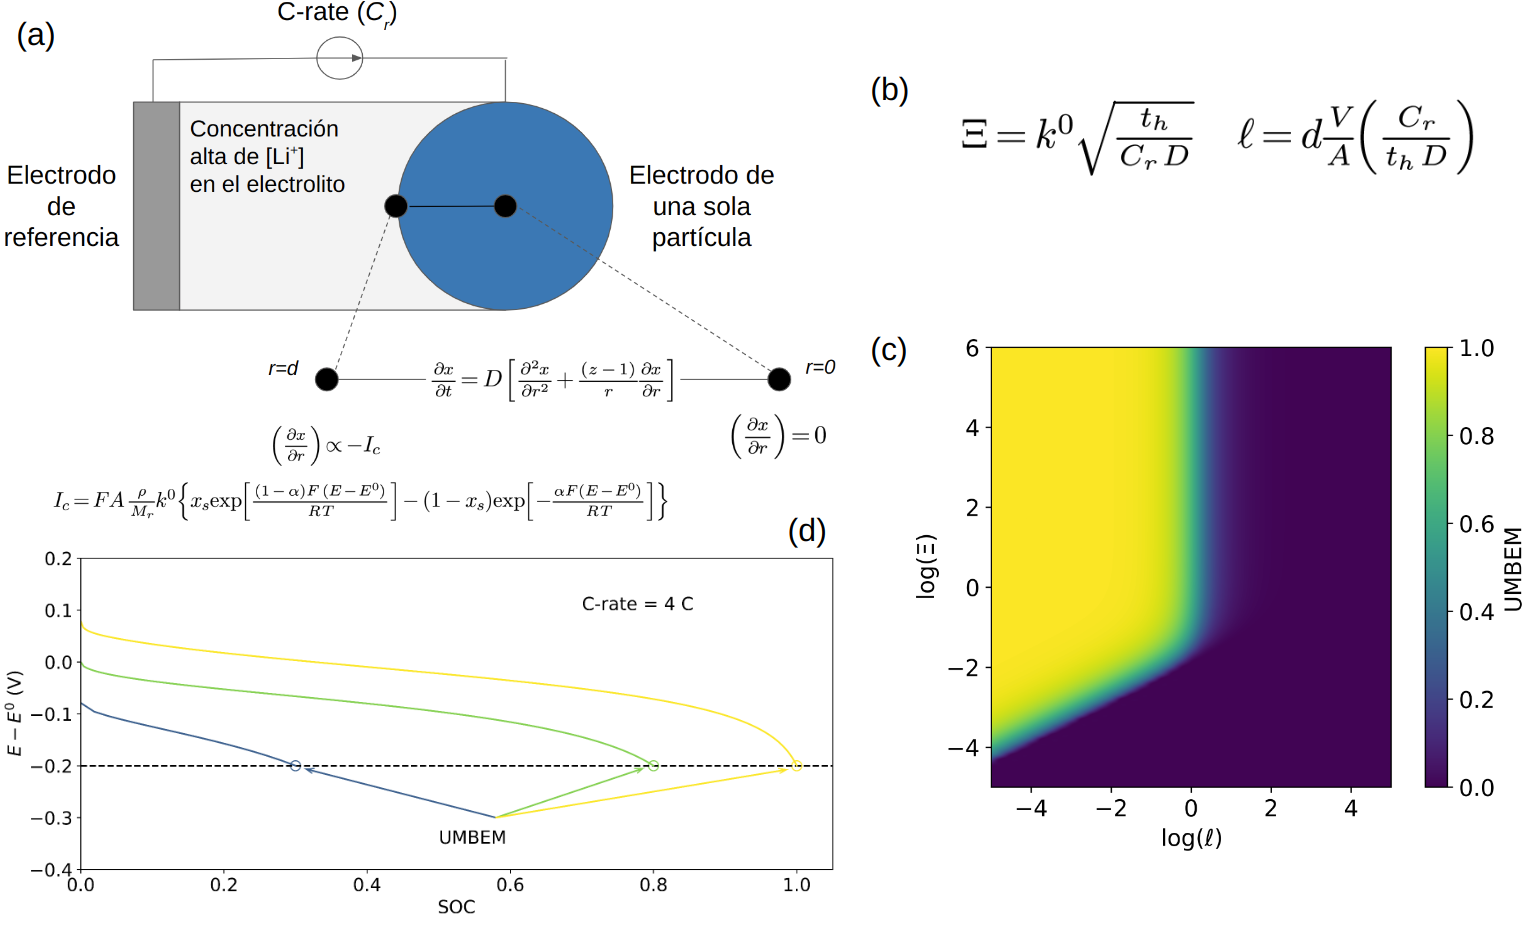
\includegraphics[width=\textwidth]{FastCharging/umbem/explicacion/explicacion.png}
    \caption{Esquema del modelo utilizado para construir el diagrama y hacer 
    las predicción de carga rápida. (a) Modelo de una sola partícula. (b) 
    Parámetros adimensionales que se derivan de las condiciones del modelo 
    en la sección \ref{s:derivparam}. (c) Diagrama universal construido con 
    simulaciones galvanostáticas que representa el estado de carga alcanzado para 
    un potencial de corte de 200 mV y una geometría esférica. (d) Ilustración
    de la métrica UMBEM que se presenta en este capítulo.}
    \label{fig:explicacion}
\end{figure}

La Tabla \ref{t:dataset} resume la información experimental ($d$, $D$) que se 
requiere para evaluar con la métrica UMBEM los distintos sistemas, la misma fue 
extraída de la referencia \cite{xia2022}. Sin embargo, como la discusión se 
realizará en el contexto del modelo esquematizado en la Figura 
\ref{fig:explicacion}, también se necesita considerar la constante cinética $k^0$.
Valores experimentales típicos para este parámetro fundamental se encuentran en 
un intervalo que va desde $10^{-5}$ hasta $10^{-9}$ cm/s \cite{gavilan2020kinetic}, 
por lo cual se utiliza un valor intermedio de $10^{-7}$ cm/s para todos los 
materiales. La C-rate fue fijada a 4 C, que se corresponde con 15 minutos, 
de acuerdo a la propuesta del USABC. 
\begin{table}[h!]
    \centering
    \caption{Datos experimentales de distintos sistemas requeridos para evaluar 
    la métrica UMBEM.}
    \setlength\extrarowheight{2pt}\stackon{%
    \begin{tabular}{l c c r}
        \toprule
        \textbf{Material} & 
        \textbf{$d$ [$\mu$m]} &  
        \textbf{$D$ [cm$^2$/s]} &  
        \textbf{Referencia} \\ 
        \midrule
                  & 10 & 7.8$\times10^{-11}$ & \cite{zhang2020ni} \\
        Ternarios & 8 & 1.7$\times10^{-11}$--6.5$\times10^{-9}$ & \cite{yang2012determination} \\
                  & 2--5 & 1$\times10^{-11}$--3$\times10^{-11}$ & \cite{ashton2020multiple} \\
        \midrule
            & 5--10 & $10^{-11}$--$10^{-7}$ & \cite{dokko2001kinetic} \\
            &  & $10^{-10}$--1.5$\times10^{-9}$ & \cite{barker1996electrochemical} \\
        LCO & 0.5 & $10^{-10}$--$10^{-8}$ & \cite{balke2010nanoscale} \\
            & 1--5 & 4$\times10^{-11}$--1.7$\times10^{-10}$ & \cite{zhu2019new} \\
            & 0.1 & 1.34$\times10^{-11}$ & \cite{rano2019characterization} \\
        \midrule
            & 0.2 & 9.04$\times10^{-11}$ & \cite{wang2020improved} \\
            &  & 1.5$\times10^{-12}$ & \cite{kamenskii2019advantages} \\
        LMO & 0.3 & 2.97$\times10^{-12}$ & \cite{zhou2019lixmn2o4} \\
            & 2--5 & 1.57$\times10^{-7}$ & \cite{mao2017nanoparticle} \\
            & 10 & $10^{-9}$--$10^{-7}$ & \cite{marzec2002conduction} \\
        \midrule
            & 0.1 & 1.07$\times10^{-12}$ & \cite{weng2020situ} \\
            & 0.2 & 1.3$\times10^{-14}$--1.7$\times10^{-14}$ & \cite{budumuru2018mn} \\
            & 0.2--0.5 & 1.11$\times10^{-12}$--6.86$\times10^{-11}$ & \cite{li2020electrochemical} \\
        LFP & 0.2--0.4 & 7.86$\times10^{-15}$--1.24$\times10^{-14}$ & \cite{li2020concentration} \\
            & 0.05--0.35 & 1.25$\times10^{-14}$--1.06$\times10^{-13}$ & \cite{zhang2019improving} \\
            & 0.1--0.5 & 1.13$\times10^{-12}$--1.83$\times10^{-11}$ & \cite{yan2020nickel} \\
            & 0.8 & 6.48$\times10^{-17}$--1.29$\times10^{-14}$ & \cite{prosini2002determination} \\
        \midrule
            & 0.45 & $10^{-12}$--1.6$\times10^{-11}$ & \cite{takami2011lithium} \\
            &  & 2$\times10^{-13}$--1.1$\times10^{-12}$ & \cite{shi2020crystal} \\
        LTO & 0.2 & 1.03$\times10^{-13}$ & \cite{kawade2018surface} \\
            & 1--5 & 5.12$\times10^{-14}$ & \cite{wang2019unveiling} \\
            & 0.09 & 1.04$\times10^{-13}$ & \cite{wang2018synthesis} \\
            &  & $10^{-12}$--$10^{-10}$ & \cite{rho2004li} \\
        \midrule
                &  & $10^{-11}$ & \cite{adams2019temperature} \\
                & 15 & 1.06$\times10^{-10}$--1.93$\times10^{-10}$ & \cite{gruet2018electrochemical} \\
                & 10 & 1.1$\times10^{-10}$--2.0$\times10^{-9}$ & \cite{cabanero2018direct} \\
        Grafito &  & 7.6$\times10^{-11}$ & \cite{umegaki2017li} \\
                &  & 4.4$\times10^{-6}$ & \cite{persson2010lithium} \\
                & 1-100 & $10^{-9}$--$10^{-5}$ & \cite{funabiki1998impedance} \\
        \bottomrule
    \end{tabular}
    }{}
    \label{t:dataset}
\end{table}
Estos cuatro valores se utilizan para calcular los parámetros adimensionales 
$\Xi$ y $\ell$ y así ubicar cada experimento en el mapa ya simulado, como se muestra
en la Figura \ref{fig:UMBEM}a. Como referencia para delimitar la región de carga
rápida del resto, se grafica la línea discontinua gris a UMBEM$ = 0.8$. Se puede
resaltar que los puntos correspondientes a un material presentan una 
dispersión mayor a lo largo del eje $\log(\ell)$ debido a la dependencia de este
parámetro con el tamaño al cuadrado de la partícula (ecuación \ref{eq:ele}). La
Figura \ref{fig:UMBEM}b muestra esta misma información en un gráfico de barras,
agrupadas por materiales. Los sistemas se encuentran ordenados por valor promedio 
de UMBEM decreciente. La línea discontinua horizontal es la misma que
en el diagrama, 0.8. Esto permite visualizar si el material cumple o no con el
criterio para ser clasificado como de carga rápida o no. Como se observa en las
Figuras \ref{fig:UMBEM}a y b, con la excepción de un dato, LCO y LMO se encuentran
en la región superior del mapa (UMBEM $\geq$ 0.8). Una mitad de los puntos del 
LTO y del LFP se encuentran en la zona de carga rápida y la otra mitad en la zona
de no-carga rápida. Por último, con la excepción de un caso de grafito, el grafito
y los materiales ternarios están fuera de la región de carga rápida.

\begin{figure}[h!]
    \centering
    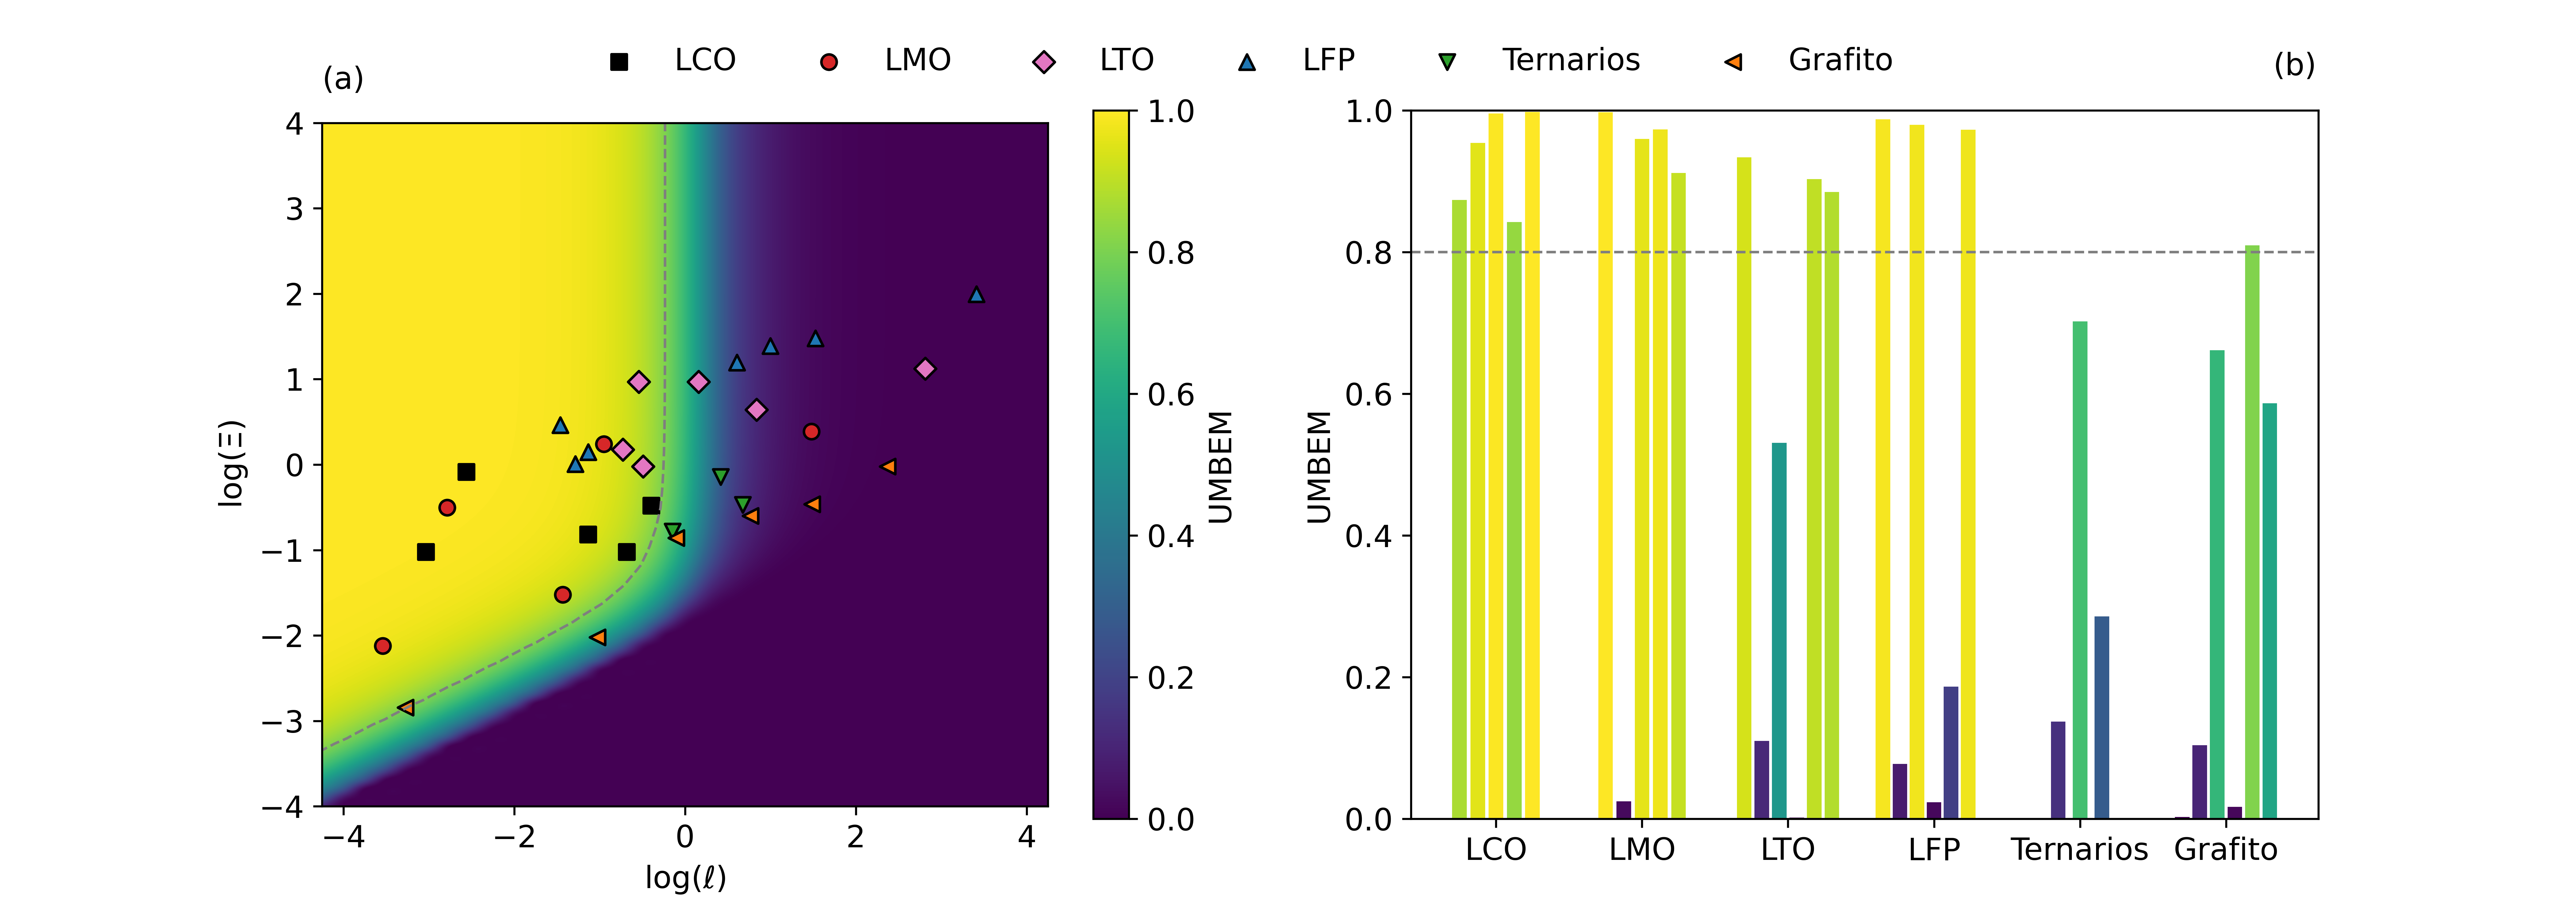
\includegraphics[width=\textwidth]{FastCharging/umbem/UMBEM.png}
    \caption{(a) Posición de cada experimento mencionado en la Tabla 
    \ref{t:dataset} en el mapa simulado representando el valor de la UMBEM. (b)
    Histograma con los valores de la UMBEM, ordenados por el desempeño promedio
    de cada sistema.}
    \label{fig:UMBEM}
\end{figure}

Xia \textit{et al.} \cite{xia2022} utilizaron los datos experimentales de $d$ y $D$
que se encuentran en la Tabla \ref{t:dataset} para calcular su FOM a cada uno 
de ellos, como se muestra en los puntos de la Figura \ref{fig:xiacomp}a. Los 
valores de la UMBEM obtenidos en la Figura \ref{fig:UMBEM} son utilizados para
colorear cada uno de ellos con el propósito de comparar ambas métricas, como
se muestra en la barra de colores de la Figura \ref{fig:xiacomp}a. A continuación
se analiza la posible existencia de una correspondencia entre ambas métricas en 
consideración, la FOM y la UMBEM. Si hubiera una correspondencia perfecta entre
las dos métricas, todos los puntos situados a lo largo de las líneas grises 
discontinuas deberían tener el mismo color. Sin embargo, puede apreciarse cómo a lo largo de
los puntos que se encuentran sobre una dada línea, el valor de la UMBEM decrece a medida que aumentan el tamaño
de la partícula y el coeficiente de difusión. De
este modo, para una relación constante de $d^2/D$, se espera un mejor desempeño 
si tanto $d$ como $D$ son menores. \todo{Esto muestra una importancia de tamaños de 
partícula menores sobre los coeficientes de difusión mayores. (YO TAMPOCO)}

\begin{figure}[h!]
    \centering
    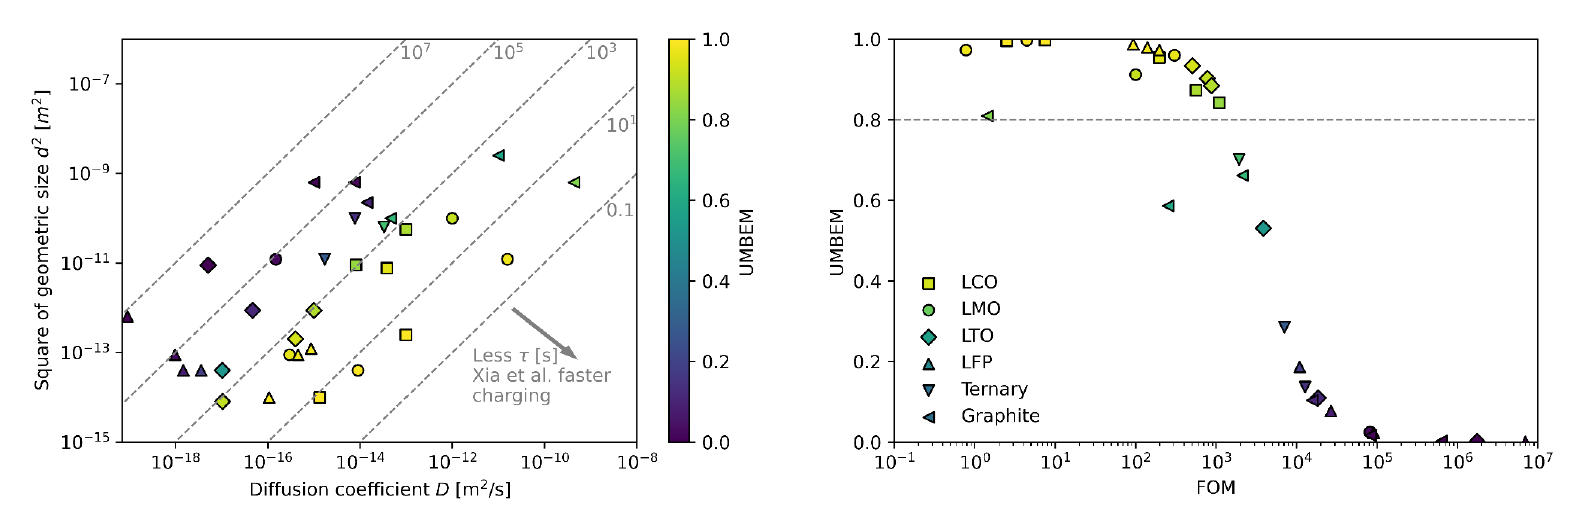
\includegraphics[width=\textwidth]{FastCharging/umbem/xiacomp.png}
    \caption{(a) Cuadro con los puntos de la Figura de Mérito (FOM) de Xia 
    \textit{et al.} coloreados de acuerdo a los valores de la UMBEM. (b) UMBEM en 
    función de FOM.}
    \label{fig:xiacomp}
\end{figure}

La Figura \ref{fig:xiacomp}b presenta la UMBEM en función de la FOM para la 
presente elección de $k^0$. Se puede observar una correlación entre ambas métricas.
Puede afirmarse que un valor de FOM menor a 10$^3$ s es considerado por la UMBEM 
como carga rápida. Sin embargo, se observan algunos valores fuera de lo esperado,
especialmente en el caso del grafito, que para dos experimentos arroja un valor de 
FOM menor a 10$^3$ s pero un valor de UMBEM menor, comparándolo con otros 
materiales como valores similares de FOM. El bajo desempeño del grafito en 
comparación a los otros materiales puede entenderse al observar los dos puntos 
del grafito que se encuentran al borde de la zona de carga rápida de la Figura 
\ref{fig:UMBEM}a. Esto muestra que a pesar de que el valor de $d^2/D$ indica
un tiempo de carga favorable (Figura \ref{fig:xiacomp}a), el coeficiente de 
difusión mayor da un valor menor de $\Xi$ (Figura \ref{fig:UMBEM}a) que resulta
en un bajo rendimiento cinético, que no es descripto por la métrica FOM.

Otra ventaja de la UMBEM sobre la FOM es que da un valor definido entre 0 y 1,
permitiendo una estimación cuantitativa de la condición de carga rápida de un
material dado. Mientras que la FOM no tiene un valor máximo y mínimo claramente
definido, ni un valor a partir del cual clasificar un material como de carga 
rápida o no.

La Figura \ref{fig:sizes}a muestra un diagrama de nivel, indicando la zona de 
carga rápida y la de carga lenta separadas por una línea correspondiente a
UMBEM$ = 0.8$. Como ya se ha dicho, este es el menor valor de carga rápida 
propuesto por el USABC. Fuera de la región de carga rápida se encuentran dos 
sistemas de ejemplo (cuadrado y círculo rojos) para dar una idea cualitativa de 
cómo un análisis guiado por el mapa puede ayudar a optimizar el desempeño de 
estos sistemas. El cuadrado que se encuentra en la parte inferior izquierda del gráfico 
podría desplazarse verticalmente para alcanzar la línea divisoria. Para que 
ese desplazamiento ocurra se necesitaría un aumento en $k^0$, como detalla la 
flecha apuntando hacia arriba en la Figura \ref{fig:sizes}a. Con respecto al 
círculo que se encuentra arriba a la derecha, se muestran dos opciones para
optimizarlo. Una consiste en moverse horizontalmente hacia la izquierda en el 
diagrama, lo cual puede lograrse reduciendo el tamaño de la partícula, como 
se muestra con la flecha horizontal etiquetada con el símbolo $d$. La otra opción
es moverse en diagonal incrementando el coeficiente de difusión, como 
muestra la flecha etiquetada con $D$. En principio, cambiar el tamaño de la 
partícula sería la más fácil de las tres opciones (cambiar $k^0$, $d$ o $D$) para 
optimizar la carga retenida, ya que experimentalmente es posible controlar este 
parámetro regulando las condiciones de síntesis de los materiales. En el párrafo
siguiente se analiza la optimización en $d$ para todos los experimentos 
considerados.

\begin{figure}[h!]
    \centering
    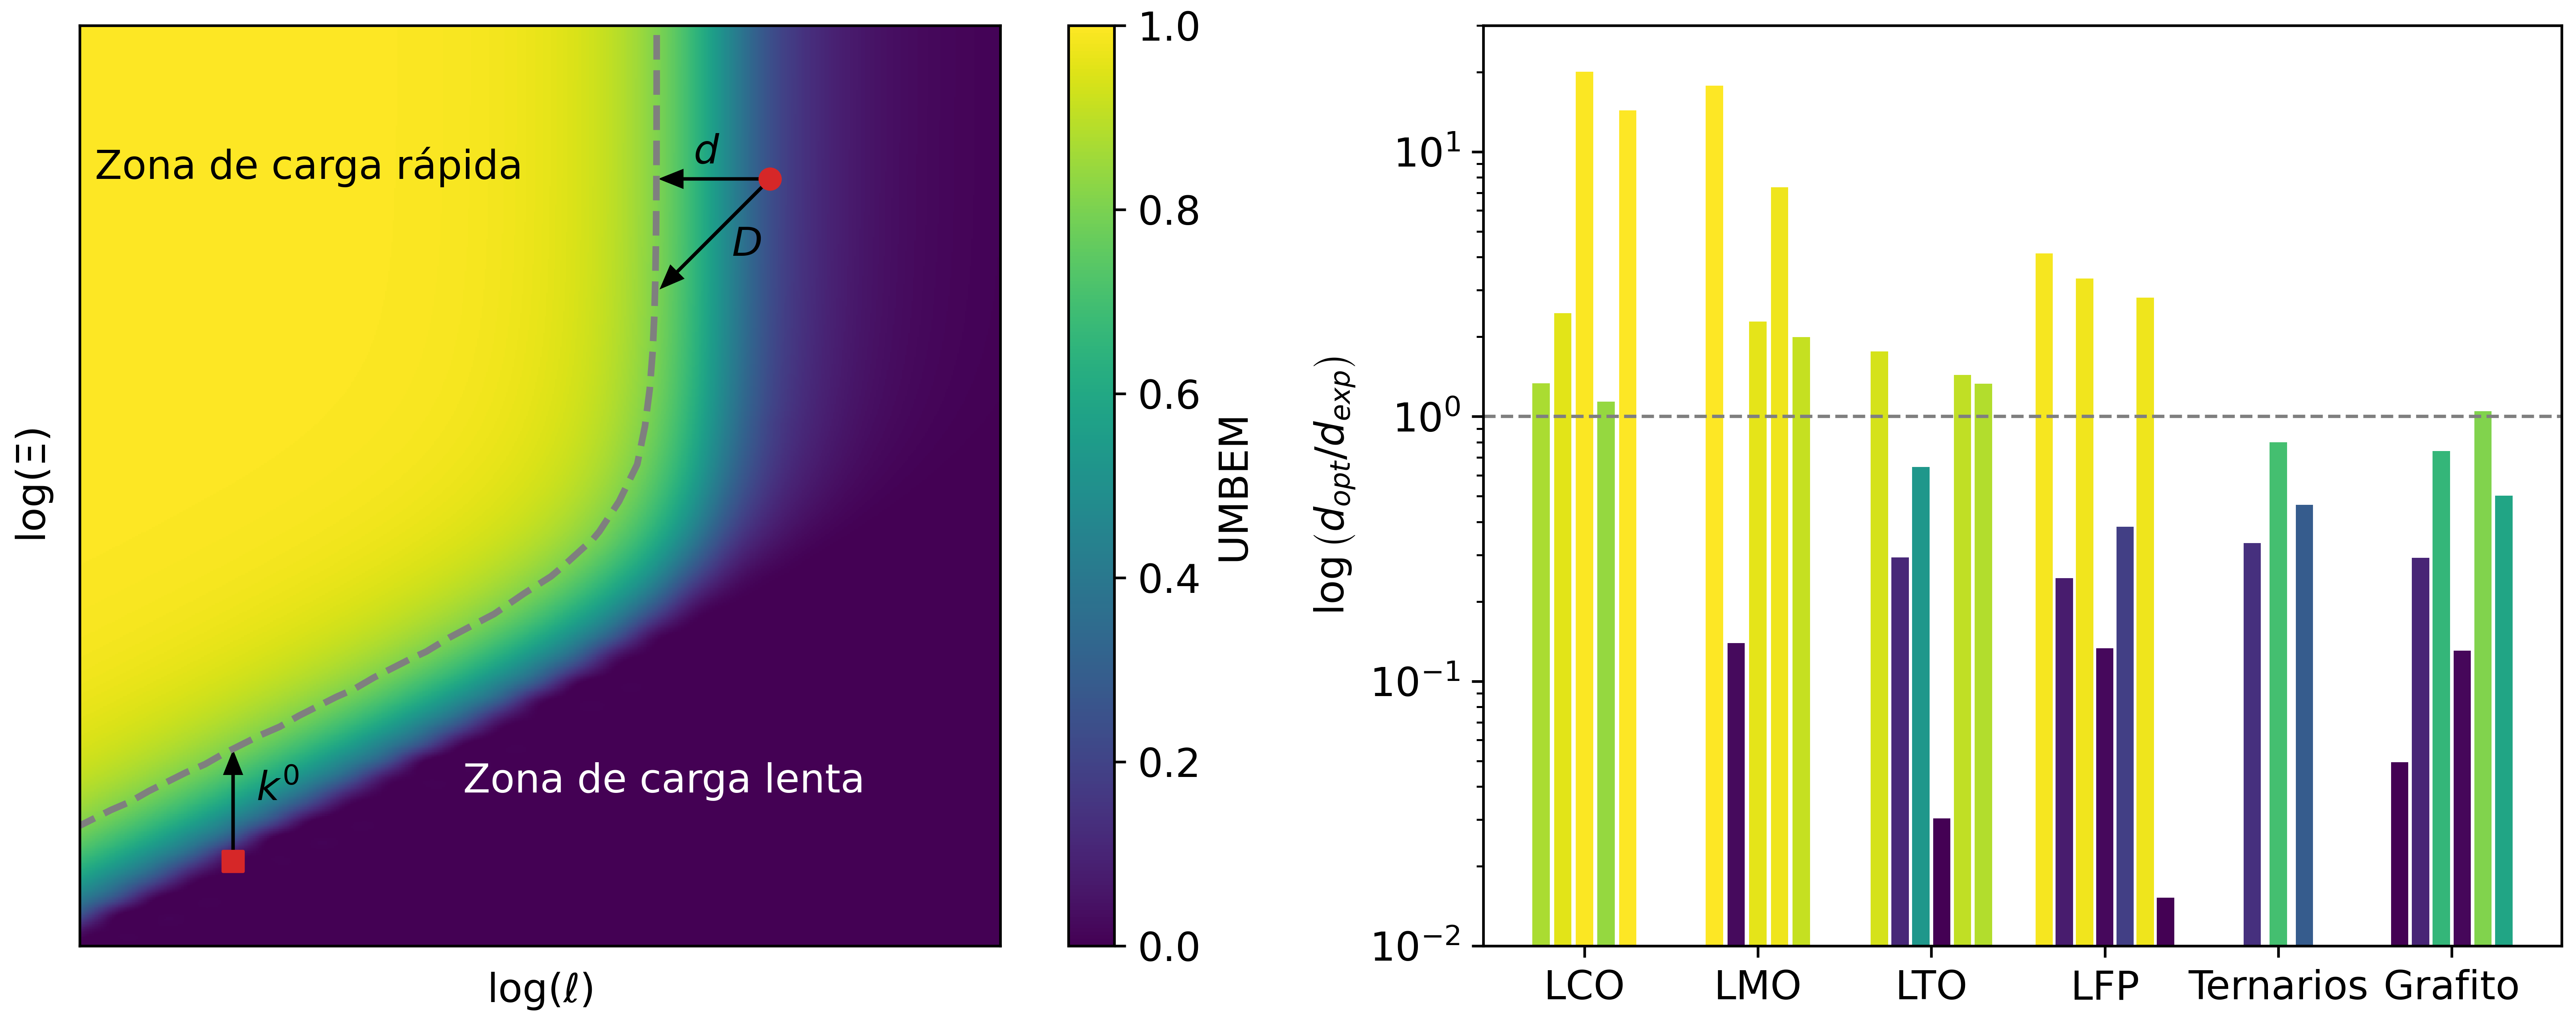
\includegraphics[width=\textwidth]{FastCharging/umbem/sizes.png}
    \caption{(a) Diagrama con las distintas maneras de optimizar el rendimiento 
    de un material. (b) Relación entre el tamaño óptimo predicho 
    ($d_{\text{opt}}$) y el experimental ($d_{\text{exp}}$) en escala logarítmica.
    El tamaño óptimo predicho es el requerido para obtener un valor de UMBEM 
    de 0.8. El color de cada barra está dado por su desempeño previo y están en 
    el mismo orden que en la Figura \ref{fig:UMBEM}a.}
    \label{fig:sizes}
\end{figure}

Se realizaron las predicciones de los tamaños óptimos de partícula para que todos 
los materiales alcancen un valor de UMBEM de 0.8, tanto para aquellos que excedían 
dicho valor como para los que estaban por debajo. Esto se presenta en al Figura 
\ref{fig:sizes}b, donde se dividieron las predicciones de los tamaños óptimos 
($d_{\text{opt}}$) por los tamaños experimentales ($d_{\text{exp}}$) para permitir
una comparación mejor entre los datos de los distintos materiales. El color de 
cada barra en el histograma está dado por su desempeño original, ya que con 
el nuevo tamaño todos tendrían el mismo color correspondiente a la UMBEM de 0.8.
La línea discontinua se corresponde al cado $d_{\text{opt}} = d_{\text{exp}}$.

\section{Concluciones del capítulo}

En este capítulo se definió una métrica universal para comparar el desempeño
de carga rápida de materiales de electrodos (UMBEM). Esta se definió como el estado de la carga 
alcanzado cuando el material se carga en condiciones de corriente constante 
durante 15 minutos. Esta métrica presenta una mejora respecto de la definida en un trabajo anterior de literatura al
considerar la difusión finita, la transferencia de carga, el tamaño de la 
partícula y el tiempo de carga. Basándose en el valor de la UMBEM para distintas 
caracterizaciones experimentales, fue posible establecer una jerarquía de 
sistemas y predecir las mejoras necesarias para \todo{clasificarlos -> encuadrarlos} como materiales de 
carga rápida.



\part{Ánodos de Silicio}

La información experimental que puede obtenerse de la estructuras de las 
distintas fases amorfas que se forman durante el ciclado de los electrodos de 
silicio es bastante limitada. Las estructuras de la red o de la interfase son 
inestables y amorfas, lo cual dificulta su caracterización mediante técnicas
experimentales tradicionales. Por ejemplo, la difracción de rayos x permitió
caracterizar la fase cristalina Li$_{15}$Si$_4$ que está presente en el electrodo
cuando este se encuentra completamente cargado ~\cite{obrovac2004}, pero esta 
técnica tiene ciertas limitaciones a la hora de estudiar estructuras amorfas 
que se encuentran en los procesos de carga y descarga. Por otro lado, el análisis
de la función distribución de a pares de Si \textit{ex-situ} de datos de rayos x
hizo posible investigar el orden a corto alcance de las estructuras amorfas
Li$_x$Si ~\cite{key2011} y proponer una explicación al mecanismo de litiación.
Sin embargo, como los elementos livianos como el Li tienen baja sensibilidad a 
los rayos x, las conclusiones están simplificadas a la formación de pequeños 
clusters de Si o de átomos de Si aislados durante la litación, lo cual limita la 
descripción de la estructura a una escala mayor.

Dentro de este contexto, las simulaciones computacionales se posicionan como una
herramienta poderosa para acceder al comportamiento microscópico de las 
estructuras de Li$_x$Si y los cambios que sufren durante la litiación. Actualmente
no existe un único modelo computacional robusto que permita estudiar todos los
diferentes procesos presentes en los electrodos de silicio, por lo que se han 
llevado a cabo distintos esfuerzos en los últimos años para estudiar este sistema.
Donde el mayor obstáculo está relacionado con la naturaleza intrínseca de 
multi-escala del silicio. A pesar de la gran precisión, los estudios de DFT se
encuentran drásticamente limitados en el número de átomos que se pueden utilizar
para modelar las estructuras complejas de las fases litiadas. Una solución a este
problema es utilizar potenciales interatómicos semi-empíricos, para los cuales 
se necesita una parametrización que se robusta y transferible. Como esta 
parametrización esta fuera de los objetivos que plantea esta tesis, en este 
capítulo se utiliza una realizada para un potencial reactivo, introducido en 
la sección \ref{s:reaxff}, para sistemas de Li-Si previamente realizada por Fan 
\textit{et al.} ~\cite{fan2013}, en la cual optimizaron el campo de fuerzas usando 
cálculos de DFT, considerando datos de las energías, distintas geometrías y cargas
de las fases cristalinas de Li, Si y aleaciones de Li-Si. En su trabajo también
utilizaron simulaciones de MD para caracterizar las propiedades mecánicas de
las estructuras amorfas de Li$_x$Si, incluyendo litiación de capa fina, compresión
biaxial, tensión y compresión uniaxial y la tensión que puede soportar el sistema 
antes de deformarse.


\section{Campo de fuerzas}

El campo de fuerzas de Fan \textit{et al.} ha sido ampliamente utilizado en 
simulaciones de MD para estudiar el proceso de litiación de distintas estructuras
de silicio, desde estructuras periódicas a nanoestructuras. Previo a la 
realización del trabajo de este capítulo, se consultó la bibliografía para 
verificar esto y asegurarnos de la transferibilidad del potencial. 

Además de los resultados reportados por Fan \textit{et al.} ~\cite{fan2013}, 
la estructura, el estrés y la difusividad fue estudiada durante la litiación de 
silicio amorfo (a-Si) y silicio cristalino (c-Si) en diferentes orientaciones 
cristalográficas ~\cite{chen2020, kim2015}. Ding \textit{et al.} ~\cite{ding2017} 
reportó la variación de la velocidad de migración en la frontera de fases y la 
difusividad de Li en función del estrés externo aplicado, exponiendo que la 
tensión acelera la razón de litiación, mientras que la compresión la retarda. Kim 
\textit{et al.} ~\cite{kim2014} realizó simulaciones de MD para caracterizar la 
evolución estructural de la frontera de fases entre c-Si, con diferentes planos 
de orientación, con una fase amorfa de litiación máxima. Posteriormente, Fan 
\textit{et al.} ~\cite{fan2018} estudió nanoestructuras, computando la respuesta
mecánica de nanopilares de c-Si en la orientación (111) durante la litiación.
Un trabajo similar, pero para la orientación (100), fue realizado por Cao 
\textit{et al.} ~\cite{cao2019}. Tang \textit{et al.} ~\cite{tang2019} investigó
la evolución y la permanencia de la porosidad de nanocapas de Si durante los 
procesos de litiación y delitiación. Ostadhossein \textit{et al.} 
~\cite{ostadhossein2015} caracterizó la litiación de nanohilos de c-Si y mostró
que este potencial ReaxFF reproduce precisamente las barreras de energía de la
migración de Li obtenidas por DFT, tanto en c-Si como en a-Si.

Este potencial no estuvo sólo limitado al uso en MD, sino que fue aplicado a otros
métodos de simulación, por ejemplo, simulaciones de Monte Carlo en el ensamble
gran canónico fueron realizadas para estudiar un ciclo de litiación y delitiación
de un electrodo de a-Si ~\cite{basu2019}. Trochet y Mousseau ~\cite{trochet2017}
caracterizaron el paisaje energético a concentraciones relativamente bajas de 
impurezas de Li en c-Si, usando una técnica de activación-relajación cinética. 
Kim \textit{et al.} ~\cite{kim2017} desarrolló un algoritmo para investigar la 
respuesta a la delitiación de una capa delgada de silicio recubierta de óxido de 
aluminio. El ReaxFF también fue combinado con otros campos de fuerza, como los
potenciales de Tersoff y Lennard-Jones, para simular la litiación de 
nanopartículas de Si recubiertas con carbono, que permitieron observar una 
correlación entre el crecimiento del estrés y la densidad de carga 
~\cite{zheng2019,zheng2020}. Propiedades mecánicas de interfase Si/SiO$_2$ litiada 
fueron reportadas por Verners y Simone ~\cite{verners2019}. 

El estudio de las propiedades electrónicas no es posible con el uso del ReaxFF ya
que es una de sus limitaciones. Sin embargo, de la discusión previa, puede 
observarse que ha sido capaz de predecir un número importante de propiedades del 
sistema Li-Si.


\section{Configuraciones iniciales}

\subsection{Estructuras cristalinas}

En este capítulo se estudian las propiedades de las estructuras amorfas Li$_x$Si
para distintos valores de $x$ en el rango que va de 0.21 a 4.2. Para algunos de
estos existen concentraciones a las cuales se encuentran estructuras cristalinas 
de LiSi, las cuales fueron extraídas del Materials Project 
~\cite{materials_project} (mp-1314, mp-672287, mp-569849, mp-29720) y utilizadas 
como estados iniciales. Las celdas primitivas de las estructuras cristalinas se
muestran en la figura \ref{fig:cristalinas}, donde están en orden creciente de 
concentración de Li, las mismas son Si, LiSi, Li$_{12}$Si$_7$, Li$_7$Si$_3$, 
Li$_{13}$Si$_4$, Li$_{15}$Si$_4$, Li$_{21}$Si$_5$ y Li, los enlaces de Si-Si 
están graficados si la distancia entre dos de estos átomos es menor a 2.5\AA. En 
la estructura de LiSi se tiene una remanencia del diamante de Si en los enlaces, 
en Li$_{12}$Si$_7$ hay dos tipos de clusters de átomos de Si, pentagonos y 
estrellas, en Li$_7$Si$_3$ los átomos de Si se encuentran en mancuernas, en 
Li$_{13}$Si$_4$ se tienen las mismas mancuernas junto a algunos átomos aislados y, 
por último, en Li$_{15}$Si$_{4}$ todos los átomos de Si se encuentran aislados,
al igual que en la Li$_{21}$Si$_5$. Estas estructuras cristalinas fueron 
observadas a temperaturas altas ~\cite{wen1981}, pero no se encuentran en el 
funcionamiento de una batería ~\cite{obrovac2004}. Sin embargo, sus posiciones 
pueden tomarse como iniciales para simular a las concentraciones correspondientes.
\begin{figure}[th]
    \centering
    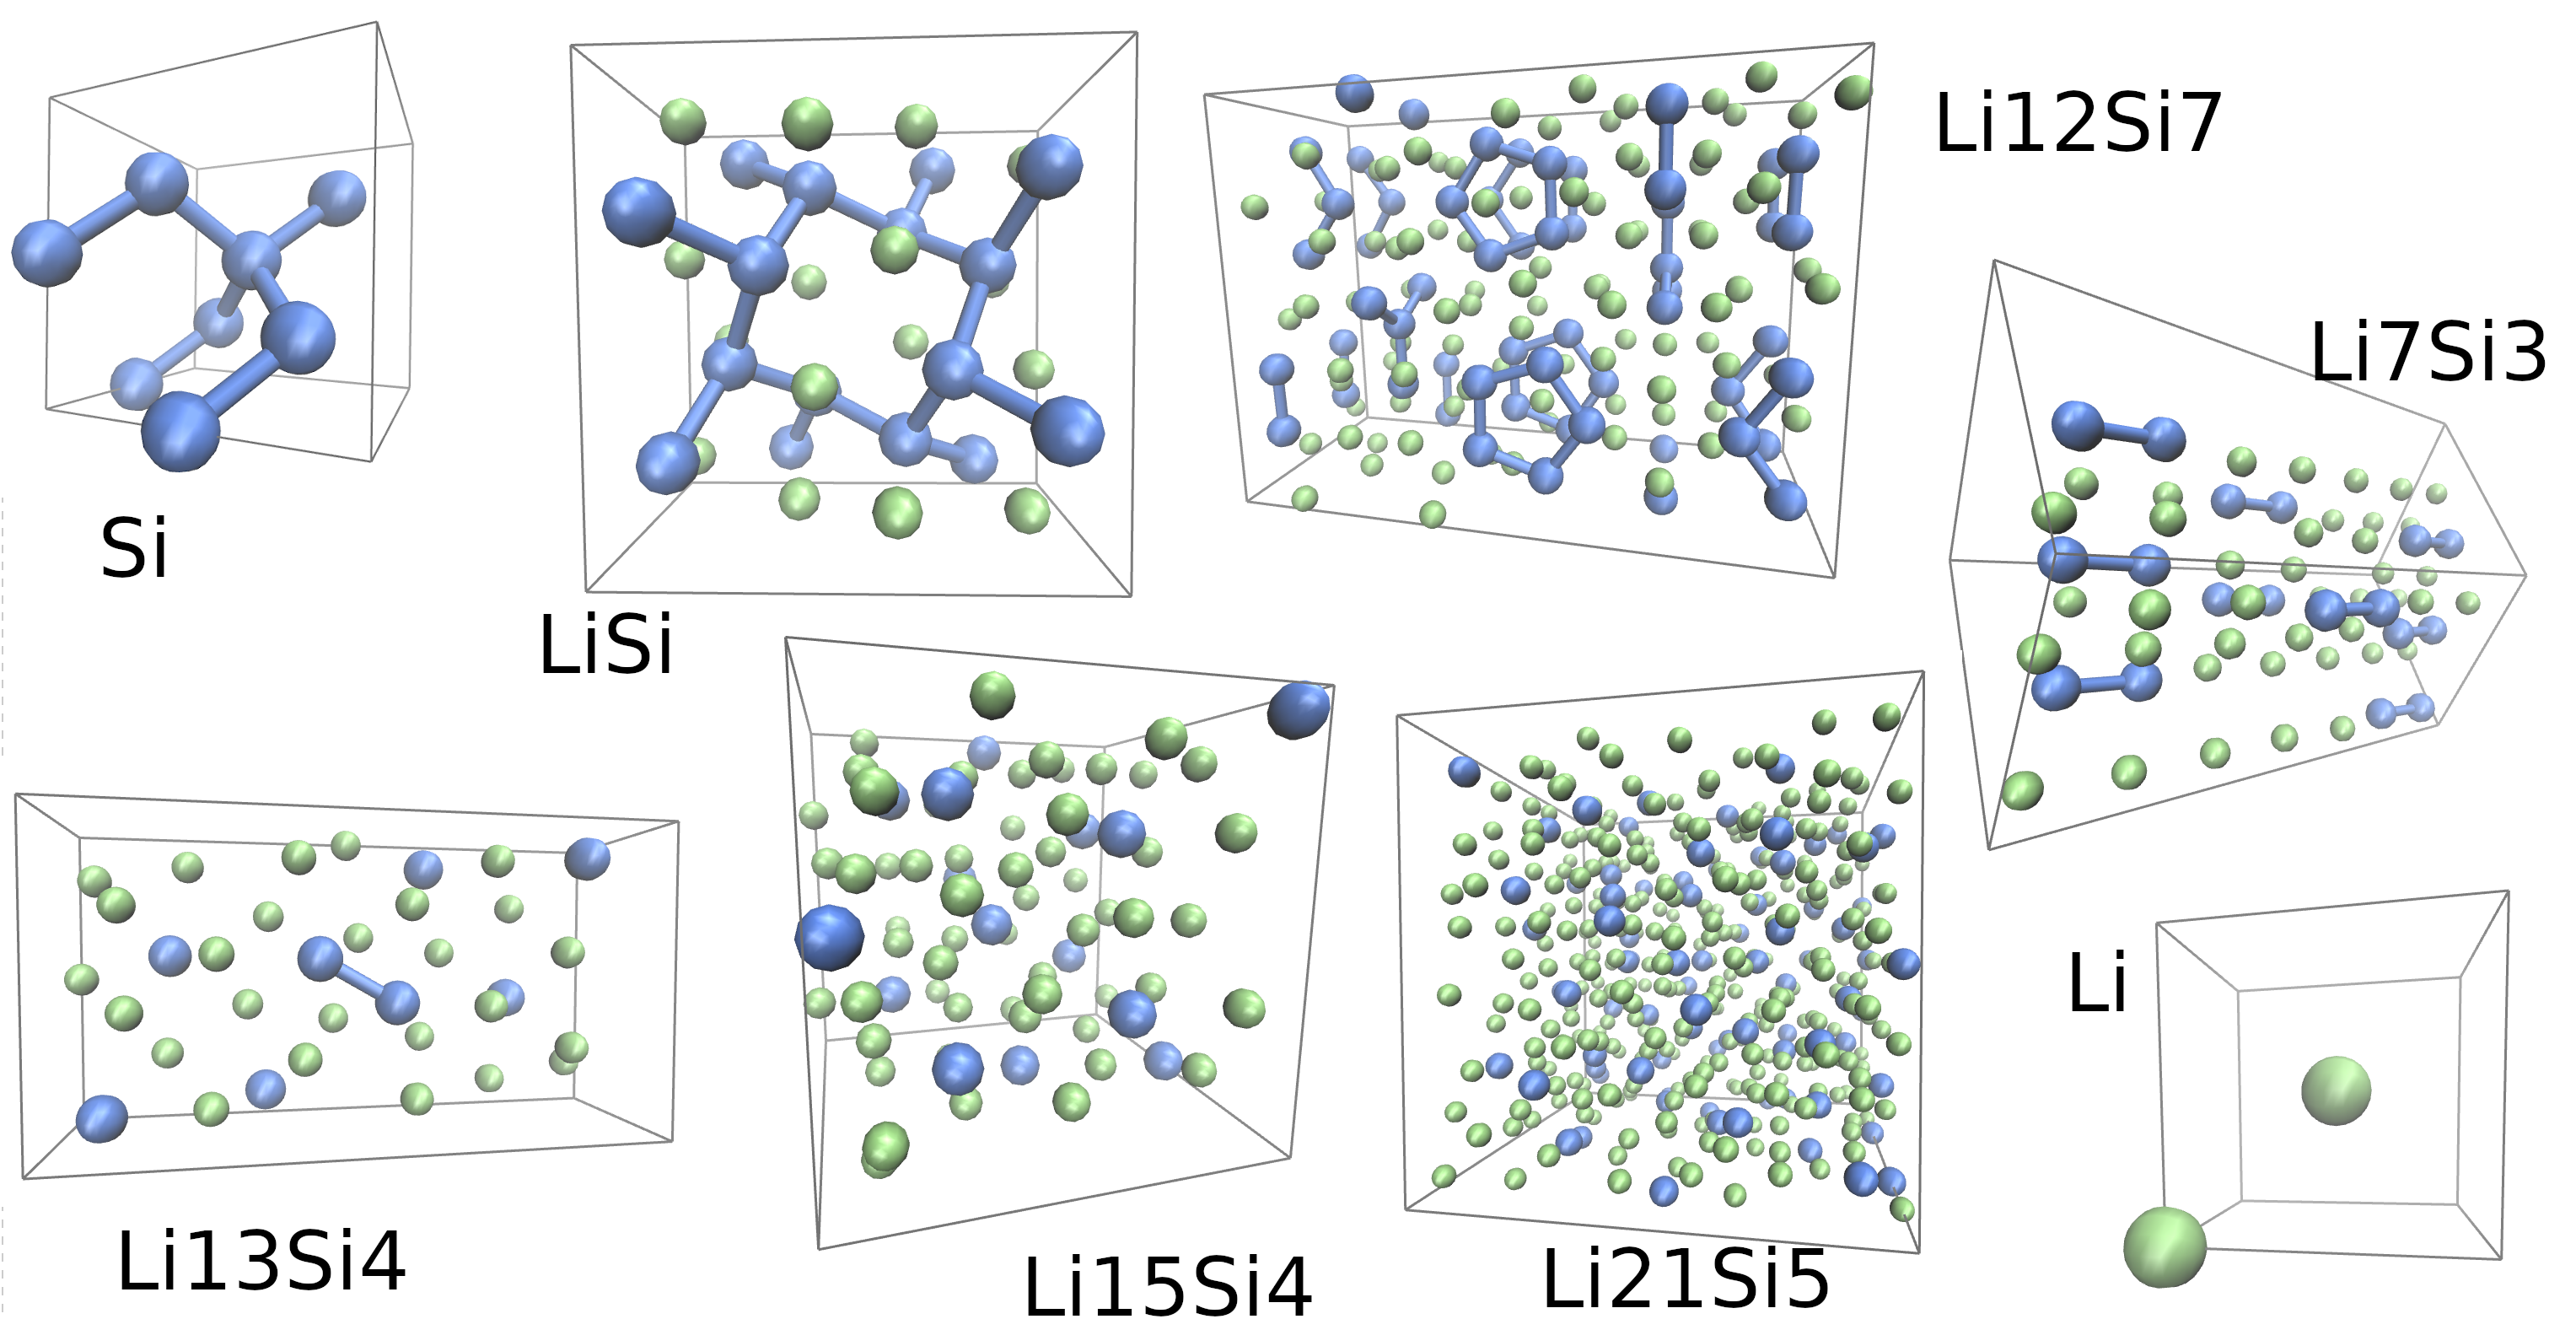
\includegraphics[width=\textwidth]{caracterizacion/cristalinas.png}
    \caption{Estructuras cristalinas de LiSi. Las estructuras no están a escala 
    entre sí. Los átomos de Si se muestran en azul y los de Li en verde, mientras
    que la celda periódica en gris.}
    \label{fig:cristalinas}
\end{figure}

\subsection{Protocolo de delitiación}

Para obtener configuraciones iniciales para valores de $x$ distintos a los de las 
cristalinas se siguió un protocolo de delitiación en el cual se selecciona la 
estructura cristalina más cercana con un valor de $x$ superior al deseado,
se le extrae un átomo de Li de manera aleatoria y se realiza una dinámica en el 
ensamble NPT durante 2 ps para relajar el volumen. Para estas simulaciones se 
utilizó el termostato de Nosé-Hoover ~\cite{nose1984a, nose1984b, hoover1985} a
300.0 K y un barostato a 0.0 atm con un paso temporal de 1 fs utilizando el
software \path{LAMMPS} ~\cite{lammps1, lammps2}. La extracción del átomo de Li y
la simulación en el ensamble NPT fueron repetidas hasta alcanzar una concentración
deseada. Por último, la estructura con la menor presión absoluta fue seleccionada
como estado inicial para la exploración acelerada de mínimos locales que se 
introduce en la siguiente sección.


\section{Exploración acelerada de mínimos locales}

Las simulaciones de MD tienen un gran poder predictivo para el estudio de 
procesos presentes en las baterías de litio, sin embargo, las escalas de tiempo
están limitadas de unos pocos ns o $\mu$s. El número de operaciones que se 
necesita para alcanzar las escalas de tiempo de la operación de una batería 
experimental son prohibitivos, incluso considerando el uso de potenciales 
semi-empíricos como el ReaxFF en supercomputadoras. Como consecuencia de esto,
la MD usual no es suficiente para una exploración del espacio de las fases y las
estructuras de Li-Si observadas van a estar cercanas a las configuraciones 
iniciales mientras que en el sistema real probablemente pueden aparecer otras
configuraciones. Un método simple y poderoso para acelerar la exploración de 
mínimos locales en sistemas moleculares es el templado simulado 
~\cite{kirkpatrick1983}, en el cual básicamente se busca mejorar la exploración
del espacio de las fases en simulaciones de MD utilizando temperaturas altas y
luego reduciéndola progresivamente hasta encontrar un mínimo de energía a 
temperatura ambiente. El templado simulado múltiple (MSA, de sus siglas en inglés 
\textit{Multiple simluated annealing}) fue utilizado para explorar y encontrar
distintas estructuras mínimas relevantes cercanas al equilibrio ~\cite{hao2015}.

La presente técnica de simulación, exploración acelerada de mínimos locales (AELM,
de sus siglas en inglés \textit{accelerated exploration of local minima}), es 
similar a la MSA pero en vez de calentar y enfriar lentamente el sistema, se 
utiliza un sesgo en la función de energía potencial para sobrepasar las barrearas
de energía y luego se realiza una minimización local, con algún minimizador local 
como gradientes conjugados o LBFGS, para encontrar el mínimo. Este método permite 
obtener muchas estructuras con energías mínimas relevantes, que son de interés a 
la hora de estudiar electrodos de Li-Si muy ciclados.

Las aleaciones de Li-Si presentan interacciones fuertes entre los átomos que las
conforman, especialmente en el enlace Si-Si donde la energía de enlace es del
orden de $\approx$2 eV ~\cite{wypych2018handbook}. Las barreras de energía 
potencial se espera que sean de ese orden de magnitud, por lo cual un muestreo de 
una MD a temperatura ambiente parece no tener solución. Para explorar ampliamente
las distintas configuraciones del sistema, $\mathbf{r}$, se transforma 
la superficie de energía potencial (PES, de sus siglas en inglés 
\textit{potencial energy surface}), $V(\mathbf{r})$, usando un potencial sesgado
\begin{equation}\label{eq:bias}
    V_b(\mathbf{r}) = V(\mathbf{r}) + (\alpha - 1) V(\mathbf{r}) = \alpha V(\mathbf{r}),
\end{equation}
donde $\alpha$ es el factor de compresión. La ecuación \ref{eq:bias} reduce las
barreras de la PES, por lo cual el tiempo de residencia en estados meta-estables
es menor que en el sistema sin sesgar y la exploración de configuraciones de 
sistemas diferentes es más eficiente y alcanzada en un tiempo de simulación 
razonable. El término $(\alpha - 1) V(\mathbf{r})$ es usualmente referido como 
la \say{función de sesgo}.

La adición de esta función de sesgo a la PES está en la base del método de 
hiper-dinámica (HD), desarrollado por Voter ~\cite{voter1997HD,voter1997method} 
para acelerar la exploración de un sistema sin perder su dinámica. En una 
simulación típica de HD, para recuperar el promedio de alguna propiedad, la 
configuración muestreada son repesadas por un factor $w$ que involucra una función
exponencial y depende del sesgo aplicado. Debido a que este sistema involucra 
cambios grandes en las energías de interacción, comparado con la energía térmica
$k_BT$, lo que implica que la función exponencial en $w$ toma valores muy grandes,
lo que hace que el procedimiento numérico sea inestable y la recuperación de 
la propiedad de interés, como la energía potencial, no sea posible. Ya que este
capítulo se centra en un estudio estructural de los sistemas, podemos descartar
el cálculo del tiempo real evolucionado en la simulación. Además, como el 
funcionamiento de las baterías luego se da a temperatura ambiente, es de esperar
que una vez que se alcanza un mínimo local el sistema explore configuraciones
cercanas a este. Por lo cual se aplica el método de gradientes conjugados (CG)
a cada configuración de la HD y de esa forma se muestrea la multiplicidad de 
estructuras.

Este método de exploración introducido en esta tesis se asemeja al templado
simulado, aunque el objetivo es explorar muchas estructuras diferentes en vez de 
encontrar el mínimo global. El templado simulado fue utilizado anteriormente
con este mismo objetivo, Hao \textit{et al.} utilizó la técnica MSA para obtener
distintas estructuras de mínima energía de péptidos ~\cite{hao2015}. En este 
método AELM se usa HD en vez de temperaturas altas para favorecer la exploración,
y se realizan múltiples minimizaciones por CG en vez de simular un enfriado. 


\section{Resultados}

Las simulaciones aceleradas fueron llevadas a cabo en el ensamble NVT a 300.0 K
con un termostato de Langevin ~\cite{schneider1978} utilizando una versión 
modificada de \path{GEMS} ~\cite{gems}. A cada estructura se le realizó una 
minimización de gradientes conjugados con el software \path{LAMMPS} 
~\cite{lammps1, lammps2}. El tamaño de los sistemas y la cantidad de estructuras 
utilizadas para obtener los siguiente resultados se presentan en la tabla 
\ref{t:siminfo}.
\begin{table}[h]
    \centering
    \caption{Información del conjunto de datos.}
    \begin{tabular}{cccccccc}
    \hline
    $x$ en Li$_{x}$Si & N$_{Li}$ & N$_{Si}$ & N$_{estructuras}$ & E$_{mean}$ / N$_T$ [eV] & E$_{std}$ / N$_T$ [eV] & $\sqrt{kT}$ / N$_T$ [eV] \\
    \hline
    0.21 & 140 & 667 & 774 & -4.399 & 0.003 & 0.0002 \\
    0.62 & 416 & 670 & 1665 & -4.002 & 0.005 & 0.0001 \\
    1.25 & 839 & 671 & 1224 & -3.521 & 0.004 & 0.0001 \\
    1.71 & 1152 & 672 & 2132 & -3.286 & 0.002 & 0.0001 \\
    2.17 & 693 & 319 & 1699 & -3.126 & 0.002 & 0.0002 \\
    2.71 & 865 & 319 & 1504 & -2.964 & 0.002 & 0.0001 \\
    3.25 & 1040 & 320 & 1464 & -2.856 & 0.003 & 0.0001 \\
    3.75 & 1080 & 288 & 2660 & -2.777 & 0.002 & 0.0001 \\
    4.20 & 1344 & 320 & 1600 & -2.717 & 0.001 & 0.0001 \\
    \hline
    \end{tabular}
    \label{t:siminfo}
\end{table}

\begin{figure}[th]
    \centering
    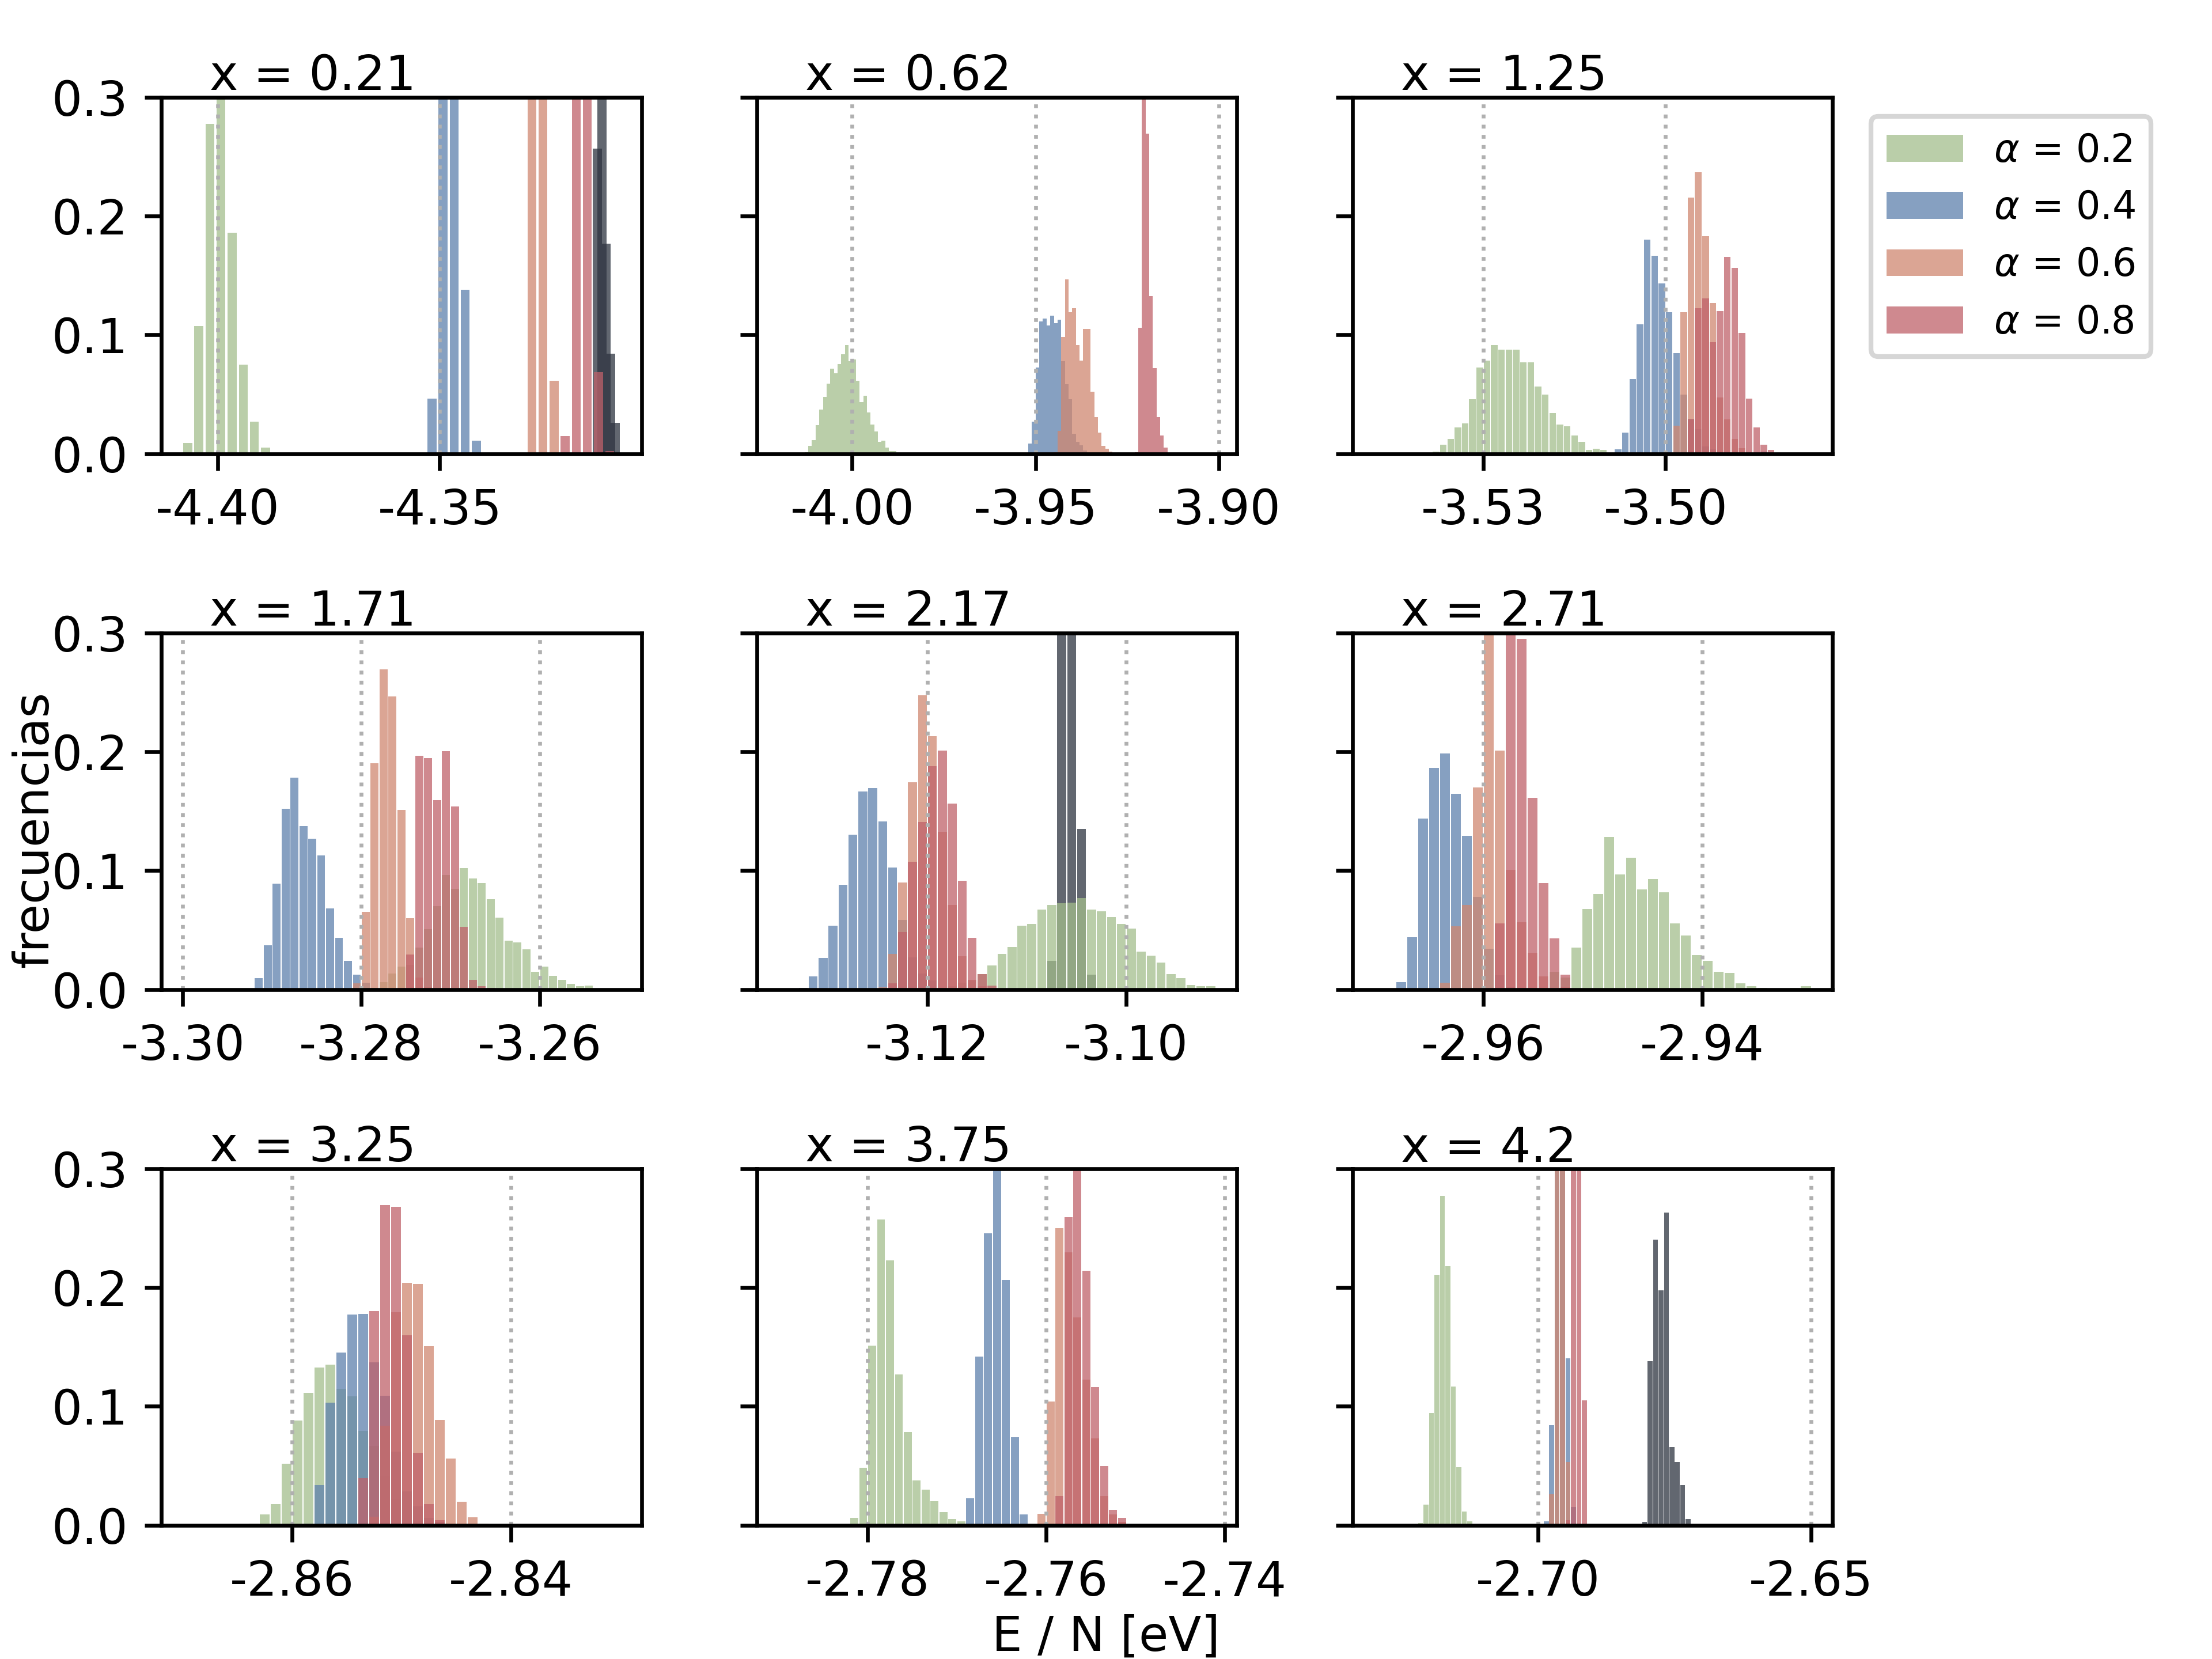
\includegraphics[width=0.8\textwidth]{caracterizacion/energias.png}
    \caption{Histogramas correspondientes a la energía potencial de las 
    estructuras obtenidas con el método AELM, con distintos valores de $\alpha$
    en la ecuación \ref{eq:bias}, para cada composición de Li$_x$Si estudiada.}
    \label{fig:energias}
\end{figure}
La figura \ref{fig:energias} muestra los histogramas para las energías mínimas
de las estructuras de Li$_x$Si obtenidas con el método AELM para los valores de
$x$ estudiados y distintos valores de compresión $\alpha$. En cada fila hay un 
histograma de energías representativo para las estructuras de concentración 
cercana, por lo cual en el análisis sólo son nombradas algunas de estas 
concentraciones. Para el primer caso, donde $x = 0.21$, se puede apreciar como el 
uso de valores más pequeños de $\alpha$ permite que estructuras con menor energía 
sean encontradas. El principal efecto de este facto $\alpha$ sobre la PES es la 
disminución de sus barreras de energía, mejorando la exploración del espacio de 
las fases. Este efecto se vuelve más drástico a medida que el valor de $\alpha$ 
tiende a cero. Para estas concentraciones representativas también se realizaron 
simulaciones de MD usuales, es decir, con un valor de $\alpha = 1$, estas no 
pueden sobrepasar las barreras de energías durante el tiempo simulado. El sistema 
permanece cercano al mínimo local asociado a la configuración inicial. Por otro 
lado, el uso de $\alpha = 0.2$ en el método de AELM resulta en un acceso rápido
a estructuras de energías menores. Un comportamiento similar se observa para 
$x = 2.17$, sin embargo, en este caso el valor más pequeño de $\alpha$ tiende a 
encontrar energías más altas que los otros casos, dando lugar a una distribución
similar a la de MD ordinaria pero con mayores fluctuaciones. Esto probablemente 
se deba a una exploración demasiado extensa, donde el sistema difunde a través
de una gran región del espacio de las fases y las minimizaciones múltiples de 
CG no son capaces de encontrar mínimos de menor energía. Por último, para la 
concentración más alta, correspondiente a un valor de $x = 4.2$, las simulaciones 
de AELM con un valor de $\alpha = 0.2$ son capaces de encontrar estructuras que 
reducen fuertemente la energía potencial del sistema. 

\begin{figure}[th]
    \centering
    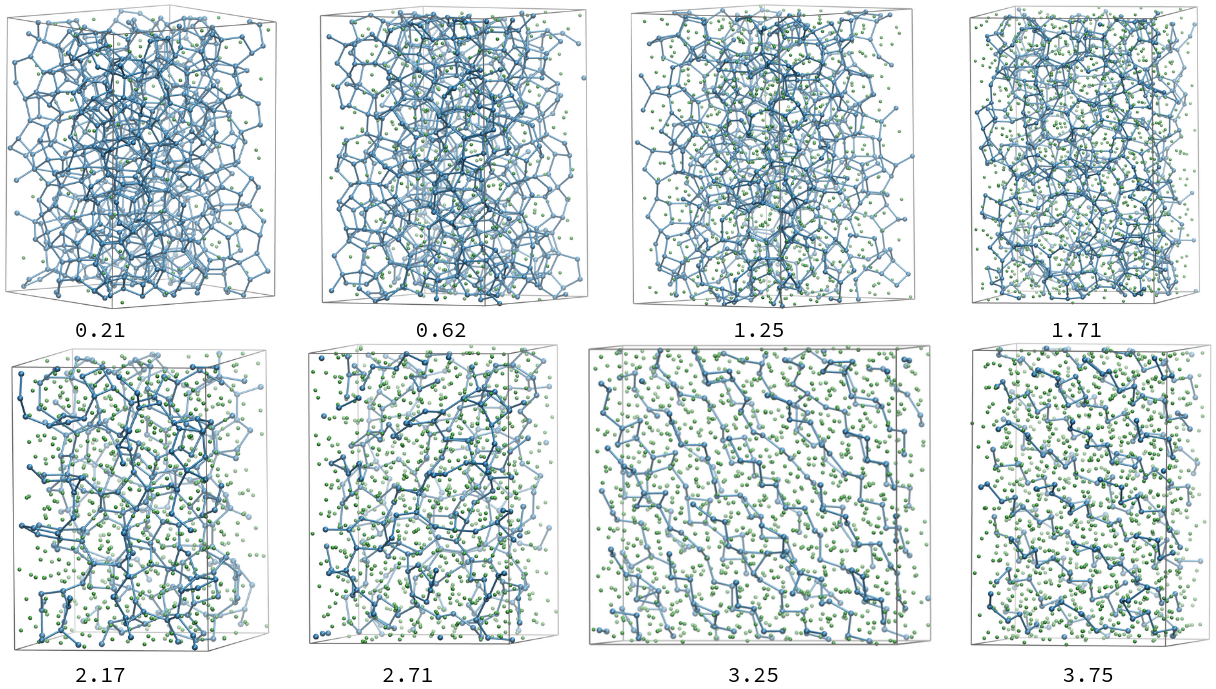
\includegraphics[width=\textwidth]{caracterizacion/amorfas.png}
    \caption{Configuración amorfa representativa de cada valor de $x$. Los átomos
    de Si se muestran en azul mientras que los de Li en verde.}
    \label{fig:amorfas}
\end{figure}
De los histogramas de la figura \ref{fig:energias} se seleccionan los factores 
de aceleración más óptimos, es decir que producen energías menores, para obtener
las propiedades estructurales que se discuten a continuación. Para estos valores
se muestra una estructura representativa a cada composición en la figura 
\ref{fig:amorfas}. Para $x = 0.21$ puede verse que la red amorfa de silicio
permanece con su estructura tetraédrica desordenada. Algunos enlaces Si-Si 
comienzan a romperse a medida que la concentración de litio aumenta, como puede
verse para las estructuras cercanas a $x = 2.17$. Por último, para las 
concentraciones más altas de litio, se alcanzan estructuras que involucran cadenas 
unidimensionales periódicas. Una estructura similar ha sido reportada por 
Ostadhossein \textit{et al.} ~\cite{ostadhossein2015}. En las próximas secciones
se caracterizan dichas estructuras.

\subsection{Comportamiento electroquímico}

\subsubsection{Cambio de volumen fraccionario}

El cambio de volumen fraccionario puede definirse utilizando una normalización 
relativa al número de átomos de Si de acuerdo a
\begin{equation}\label{eq:fvc}
    fvc = \frac{N_{Si}}{V_{Si}} \left( \frac{V_{Si,x}}{N_{Si,x}} - \frac{V_{Si}}{N_{Si}} \right),
\end{equation}
donde $V_{Si}$ y $N_{Si}$ son el volumen y el número de átomos de Si en la celda
unidad de c-Si, $V_{Si,x}$ y $N_{Si,x}$ son el volumen y el número de átomos de Si
en la celda de simulación para el valor correspondiente de $x$. En la figura
\ref{fig:fvc} se muestran los valores calculados a partir de la ecuación 
\ref{eq:fvc} para las distintas estructuras de Li$_x$Si estudiadas. En la misma 
se comparan los valores obtenidos con datos experimentales de AFM (\textit{atomic 
force microscopy}, sus siglas en inglés) medidos por Beaulieu \textit{et al.} 
~\cite{beaulieu2003} y con predicciones de DFT con un cambio volumétrico fijo 
utilizado por Chevrier y Dahn ~\cite{chevrier2009}. Los mismos muestran que el
potencial ReaxFF proporciona una tendencia correcta tanto cualitativa como 
cuantitativamente.
\begin{figure}[th]
    \centering
    \includegraphics[width=0.8\textwidth]{caracterizacion/fvc.png}
    \caption{Cambio de volumen fraccionario en función de la composición de la 
    aleación. Los valores experimentales de AFM se muestran con cuadrados azules, 
    la línea recta se corresponde con cálculos de DFT y los círculos rojos son 
    resultados de este trabajo.}
    \label{fig:fvc}
\end{figure}

\subsubsection{Voltaje}

\begin{table}[h]
    \centering
    \caption{Energías de formación obtenidas a través de la ecuación \ref{eq:fe}}
    \begin{tabular}{ccc}
    \hline
    x en Li$_x$Si & Energía de formación [eV] & Desviación estándar [eV]\\
    \hline
    0.21  &  0.5027  &  0.0037 \\
    0.62  &  0.1206  &  0.0074 \\
    1.25  & -0.1160  &  0.0096 \\
    1.71  & -0.2358  &  0.0065 \\
    2.17  & -0.3551  &  0.0075 \\
    2.71  & -0.4098  &  0.0072 \\
    3.25  & -0.5187  &  0.0126 \\
    3.75  & -0.6202  &  0.0097 \\
    4.20  & -0.6995  &  0.0075 \\
    \hline
    \end{tabular}
    \label{t:fe}
\end{table}
Las energías obtenidas pueden ser utilizadas para testear el funcionamiento del 
modelo para predecir propiedades electroquímicas, como fue sugerido por Chevrier
y Dahn ~\cite{chevrier2009}. Primero, se define la energía de formación de las 
distintas estructuras amorfas como
\begin{equation}\label{eq:fe}
    E_f(x) = E_{Li_xSi} - (x E_{Li} + E_{Si}),
\end{equation}
donde $E_{Li_xSi}$ es la energía de la aleación Li$_x$Si por átomo de Si, E$_{Li}$
y E$_{Si}$ son las energías cohesivas de Li y Si en sus fases cristalinas. Usando
la ecuación \ref{eq:fe} como aproximación a la energía de formación de Gibbs, el 
potencial \textit{versus} Li metálico de Li$_x$Si puede obtenerse a partir de
\begin{equation}\label{eq:voltaje}
    V(x) = - \frac{dE_f(x)}{dx},
\end{equation}
donde $V$ es el potencial. Los datos obtenidos así pueden compararse con valores
experimentales y computacionales previos. Las energías de formación calculadas
a partir de la ecuación \ref{eq:fe} se muestran en la tabla \ref{t:fe}. 
Realizandoles un \textit{spline} a estos valores, mostrados en el recuadro de la
figura \ref{fig:voltaje}, los valores de $V(x)$ son obtenidos de la ecuación
\ref{eq:voltaje} y son graficados en función de la composición en la figura 
\ref{fig:voltaje} con una línea roja. Para comparar, se incluye en la misma figura
las curvas experimentales medidas para la litiación y la delitiación de silicio
amorfo ~\cite{hatchard2004} y la curva teórica de cálculos de primeros principios 
~\cite{chevrier2009}. Se puede afirmar que los resultados obtenidos con el ReaxFF 
son bastante satisfactorios.
\begin{figure}[th]
    \centering
    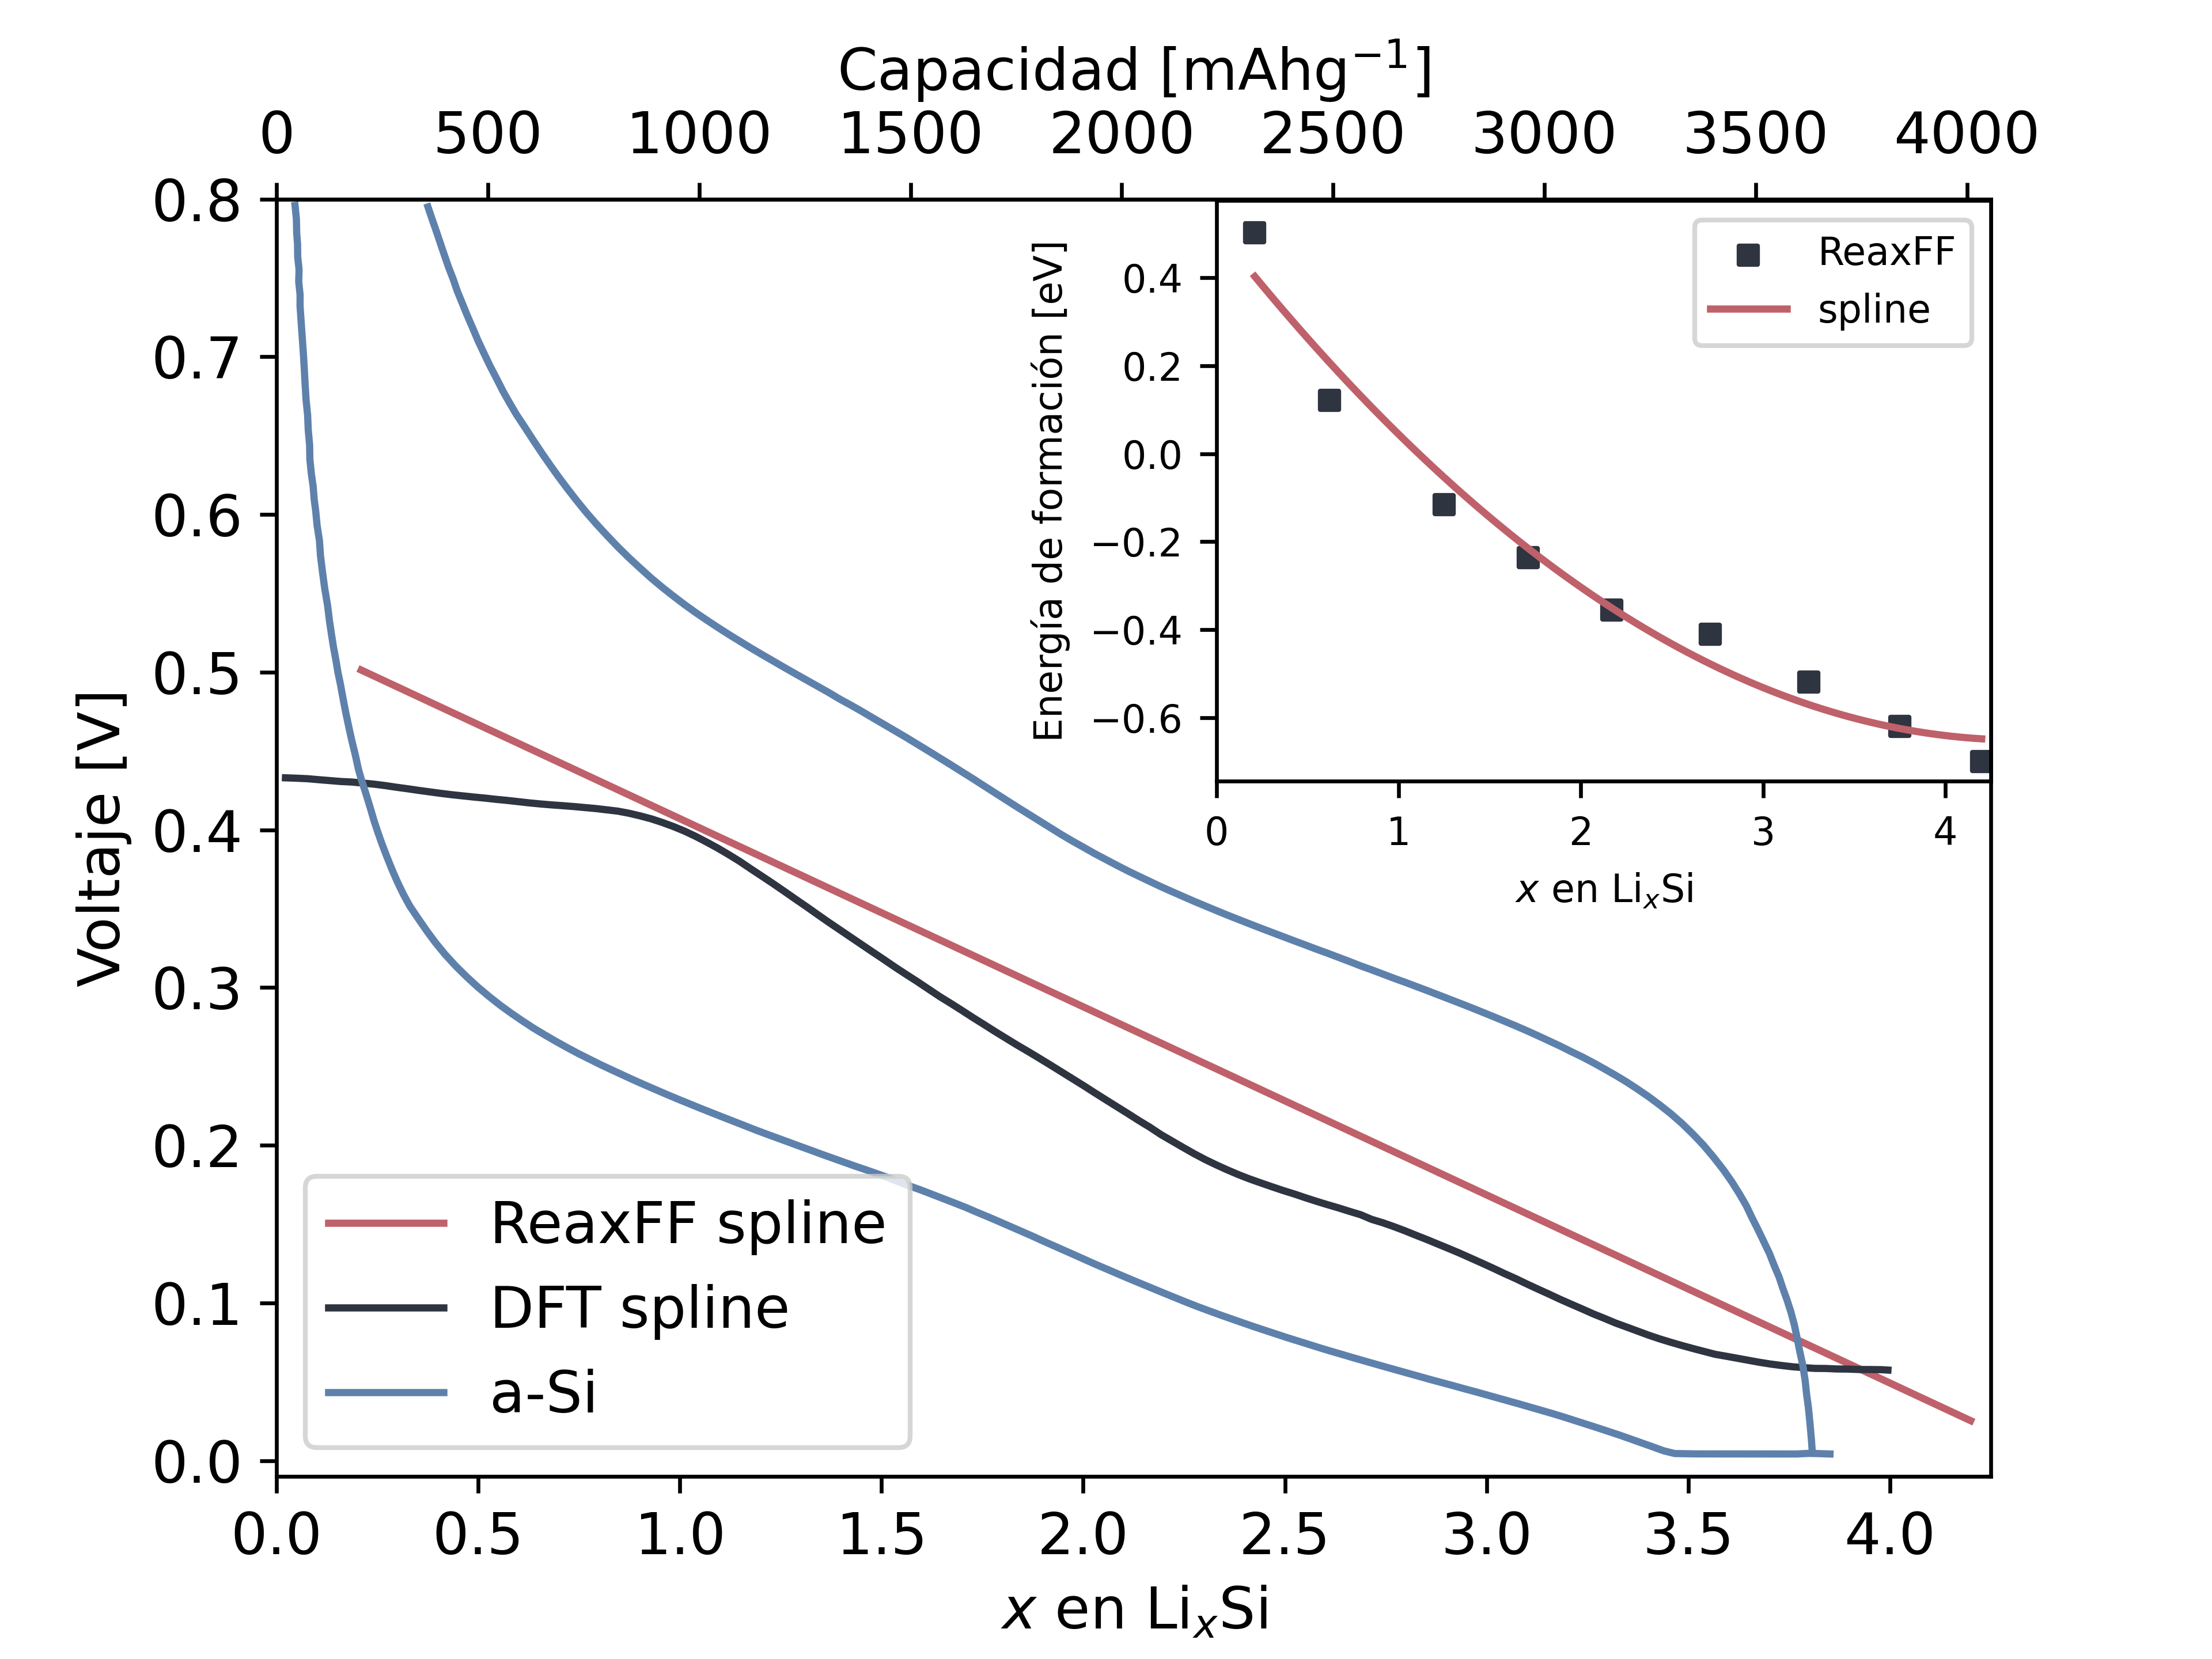
\includegraphics[width=0.8\textwidth]{caracterizacion/voltaje.png}
    \caption{Curvas potencial-concentración de la litiación de ánodos de Si.
    La línea negra se corresponde con cálculos de DFT, las líneas azules con 
    curvas medidas experimentalmente en la litiación de Si amorfo y la línea 
    roja es la derivada del \textit{spline} ajustado a los datos de la energía 
    de formación obtenidos con el ReaxFF, mostrados en el recuadro.}
    \label{fig:voltaje}
\end{figure}

\subsection{Distribución radial de a pares}

La distribución radial de a pares, introducida en la sección \ref{s:observables},
puede ser utilizada para describir la estructura de materiales amorfos. Para el 
caso de sistemas que están conformados por más de un elemento se pueden analizar 
las distribuciones radiales de a pares parciales ~\cite{lamparter1995}, donde la 
$g_{ij}(r)$ representa la RDF de los átomos $j$ a una distancia $r$ alrededor de 
los átomos centrales $i$, y que es lo mismo que considerar $g_{ji}(r)$. Las 
figuras \ref{fig:rdf-LiLi}, \ref{fig:rdf-SiSi}, \ref{fig:rdf-SiLi} muestran los
resultados obtenidos para las RDF de Li-Li, Si-Si y Si-Li, respectivamente. En
cada una de ellas se analizan los cambios en la estructura que se dan para los
distintos valores de $x$ en Li$_x$Si estudiados, las curvas se calculan sobre los
\textit{frames} minimizados de la HD.

\begin{figure}[h!]
    \centering
    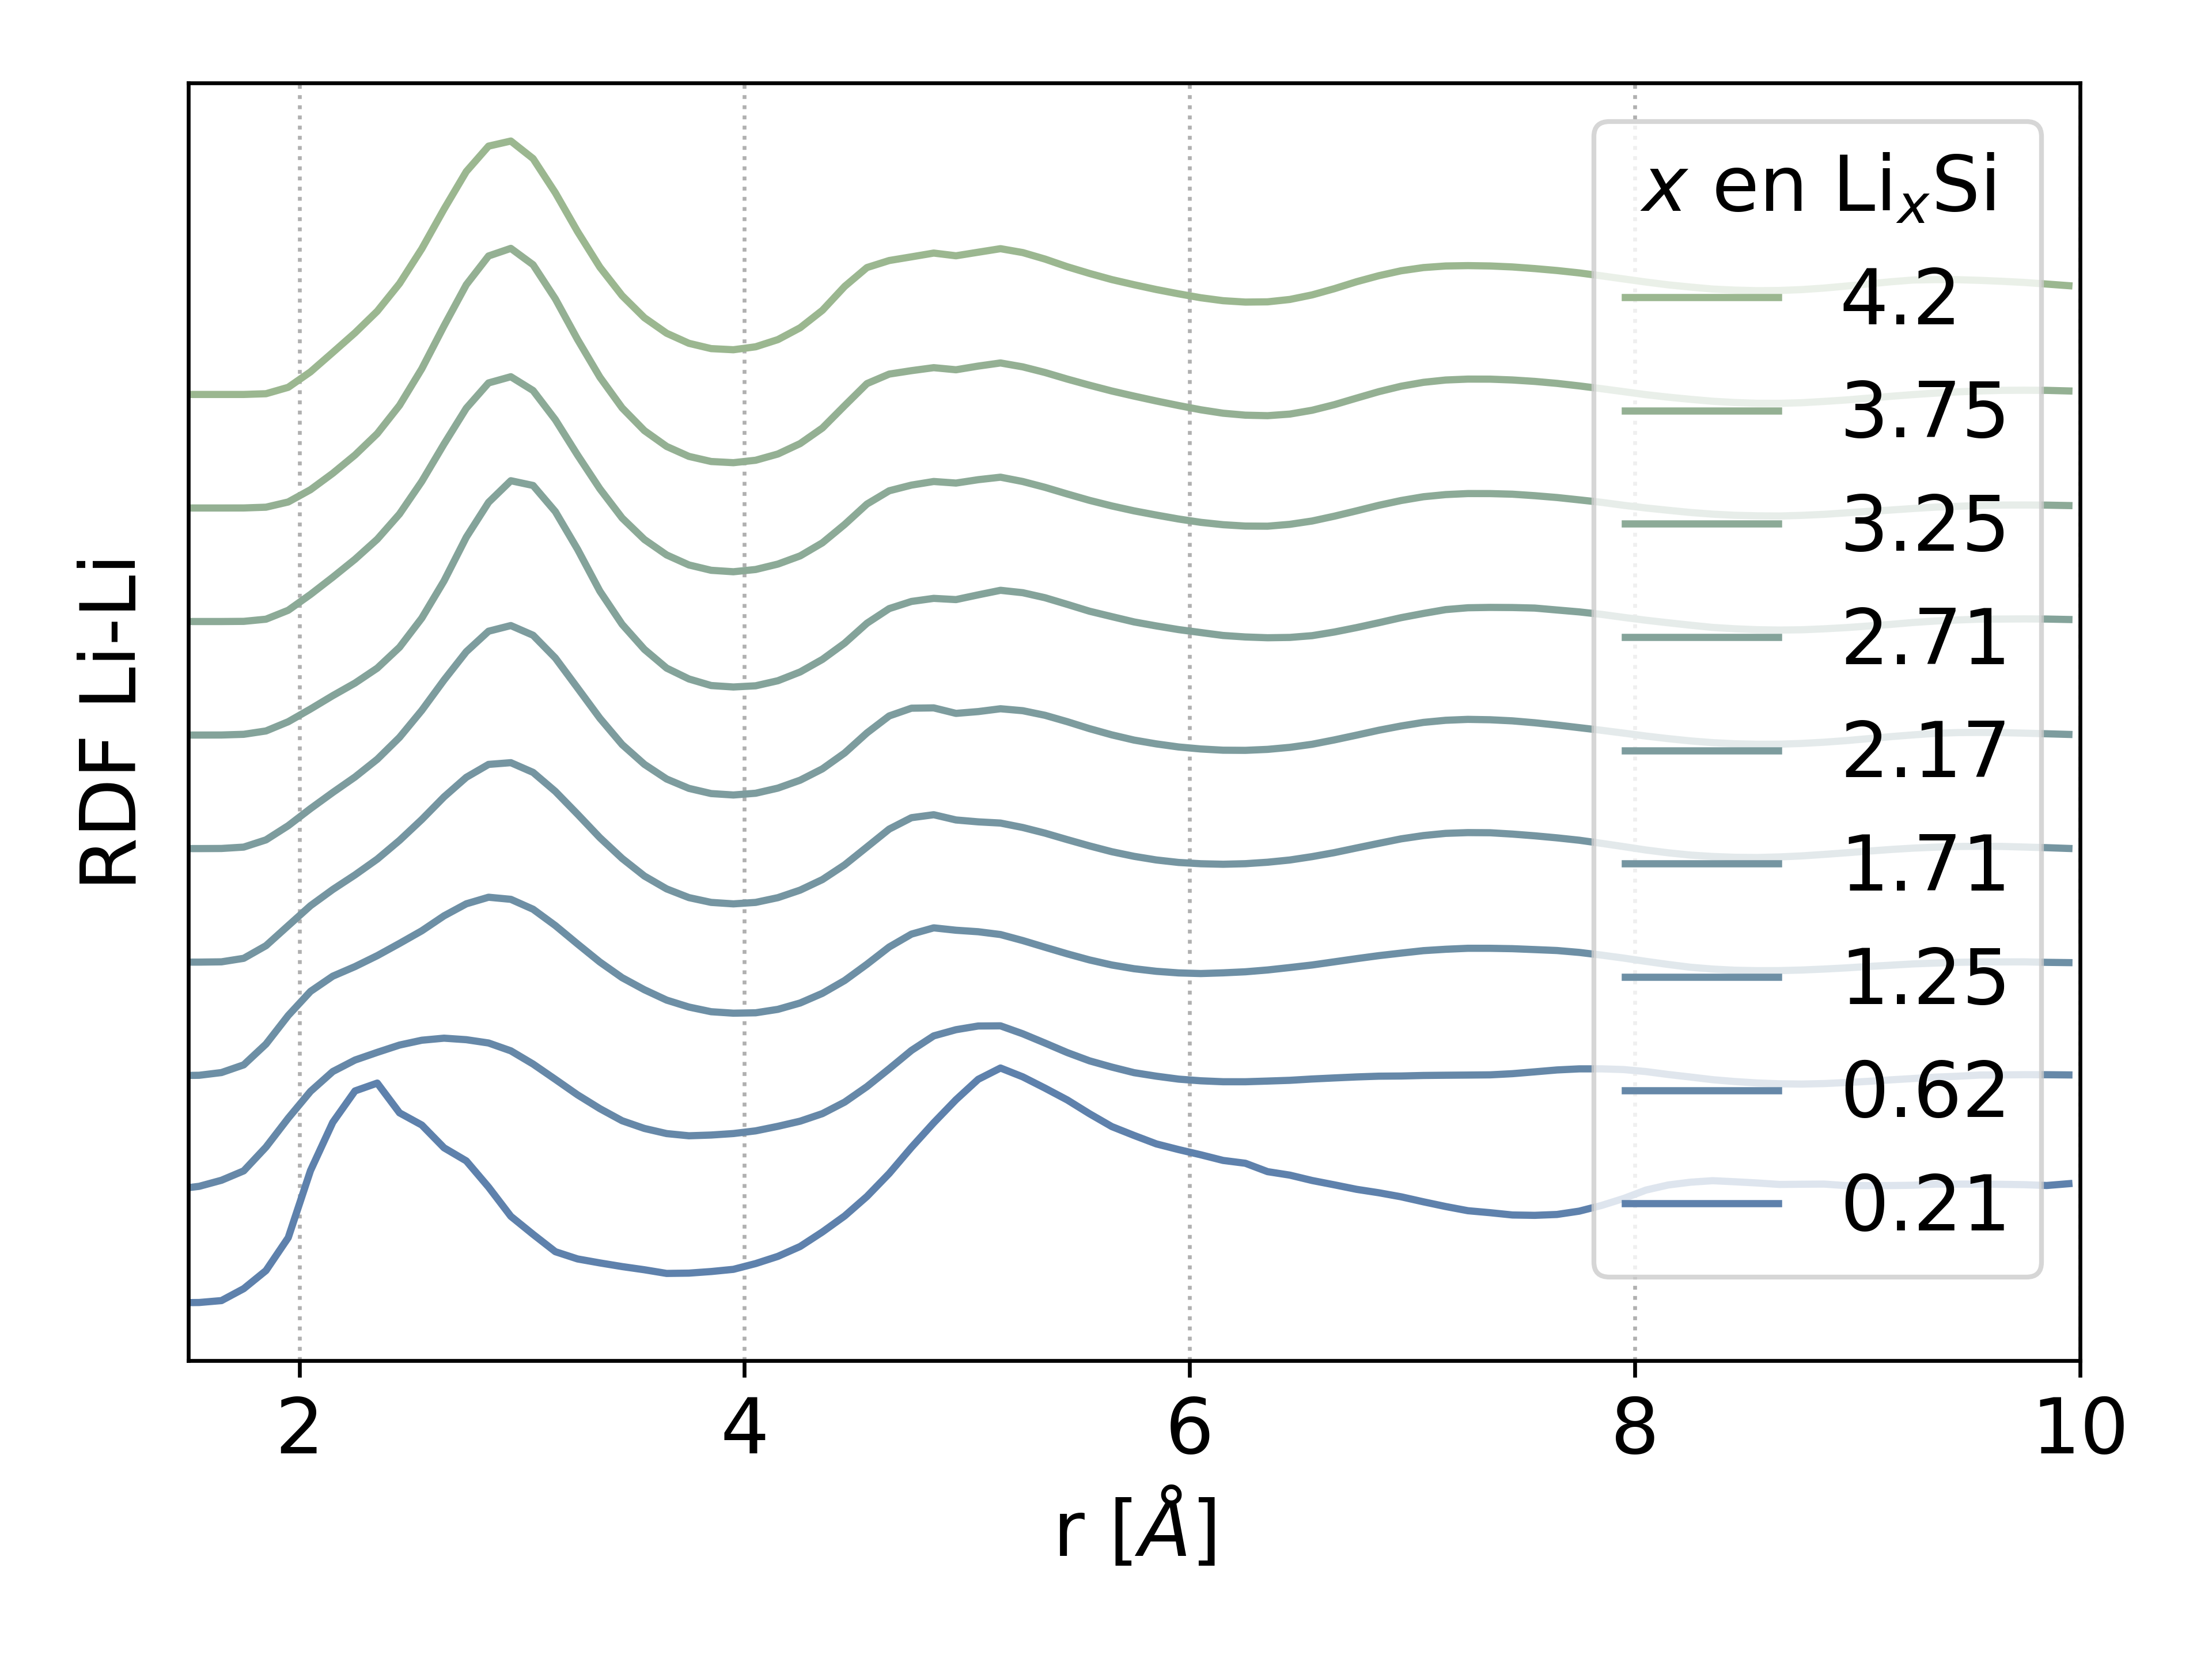
\includegraphics[width=0.8\textwidth]{caracterizacion/rdf-LiLi.png}
    \caption{Distribución radial de a pares para Li-Li de las estructuras 
    minimizadas. Cada curva se corresponde con un valor de concentración 
    distinto.}
    \label{fig:rdf-LiLi}
\end{figure}
Lo más relevante a destacar de la RDF$_{Li-Li}$ es que su primer pico comienza 
centrado en 2.45 \AA\ para las concentraciones de iones de Li más bajas y que 
luego dicho pico aumenta su posición a distancias más grandes a medida que aumenta 
$x$ hasta permanecer en 2.95 \AA\ para $x$ mayores a 1.71. La altura de este pico
aumenta en un 50\% luego de la litiación completa, relativa a la menor 
concentración.

\begin{figure}[h!]
    \centering
    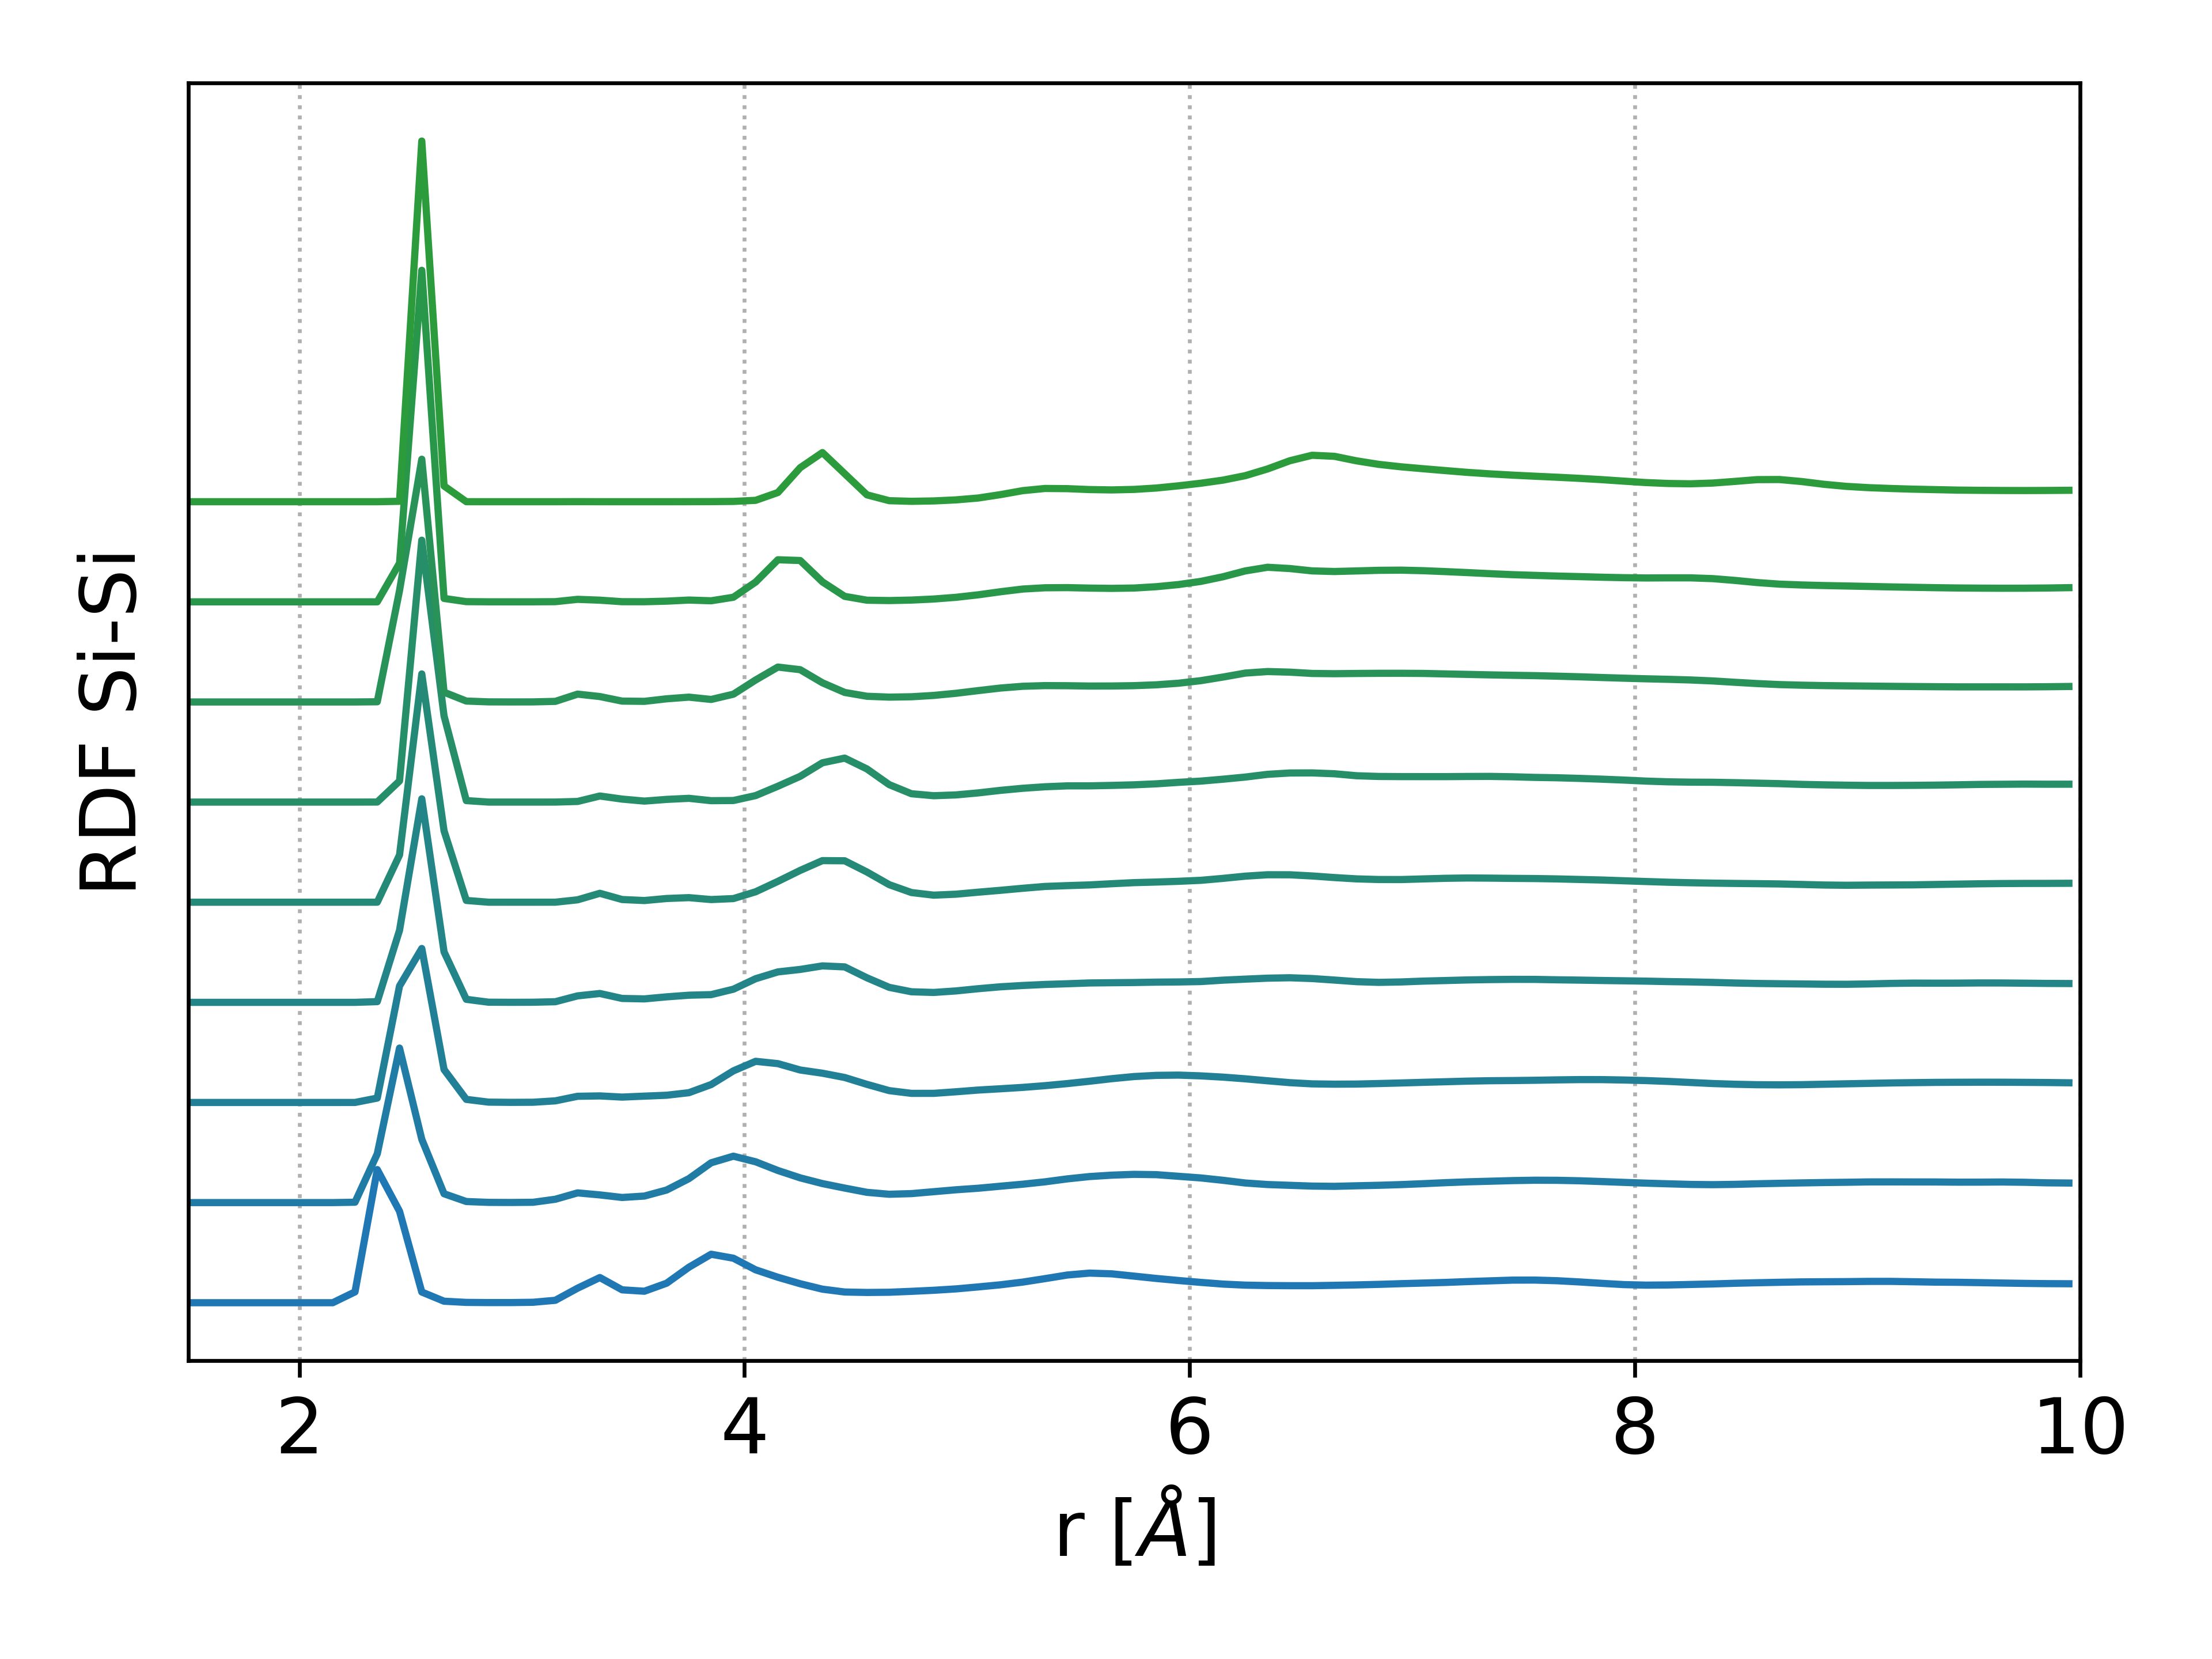
\includegraphics[width=0.8\textwidth]{caracterizacion/rdf-SiSi.png}
    \caption{Distribución radial de a pares para Si-Si de las estructuras 
    minimizadas. Cada curva se corresponde con un valor de concentración 
    distinto.}
    \label{fig:rdf-SiSi}
\end{figure}
Este mismo efecto se ve en el primer pico de la RDF$_{Si-Si}$, se observa que 
está centrado en 2.4 \AA\ para $x = 0.21$ y que luego se desplaza a distancias
mayores, después de $x = 1.25$ el centro ce encuentra entre 2.52 y 2.56 \AA.
Mientras que la altura del pico aumenta se ve un decrecimiento en en el ancho 
del pico, el valor del FWHM va de 0.14 \AA\ a 0.05 \AA\ para $x = 0.21$ y 
$x = 3.75$, respectivamente. Por otro lado, el segundo pico de la RDF$_{Si-Si}$
también se desplaza hacia distancias mayores, se divide en dos picos para valores 
de $x$ entre 0.62 y 1.71 y vuelve a comportarse como un sólo pico para para 
concentraciones mayores. Entre el primer y el segundo pico se observa un hombro,
como señaló previamente Fan \textit{et al.} ~\cite{fan2013}. Los resultados 
obtenidos para la RDF$_{Si-Si}$ están en concordancia con las mediciones 
experimentales reportadas por Key \textit{et al.} ~\cite{key2011}.

\begin{figure}[h!]
    \centering
    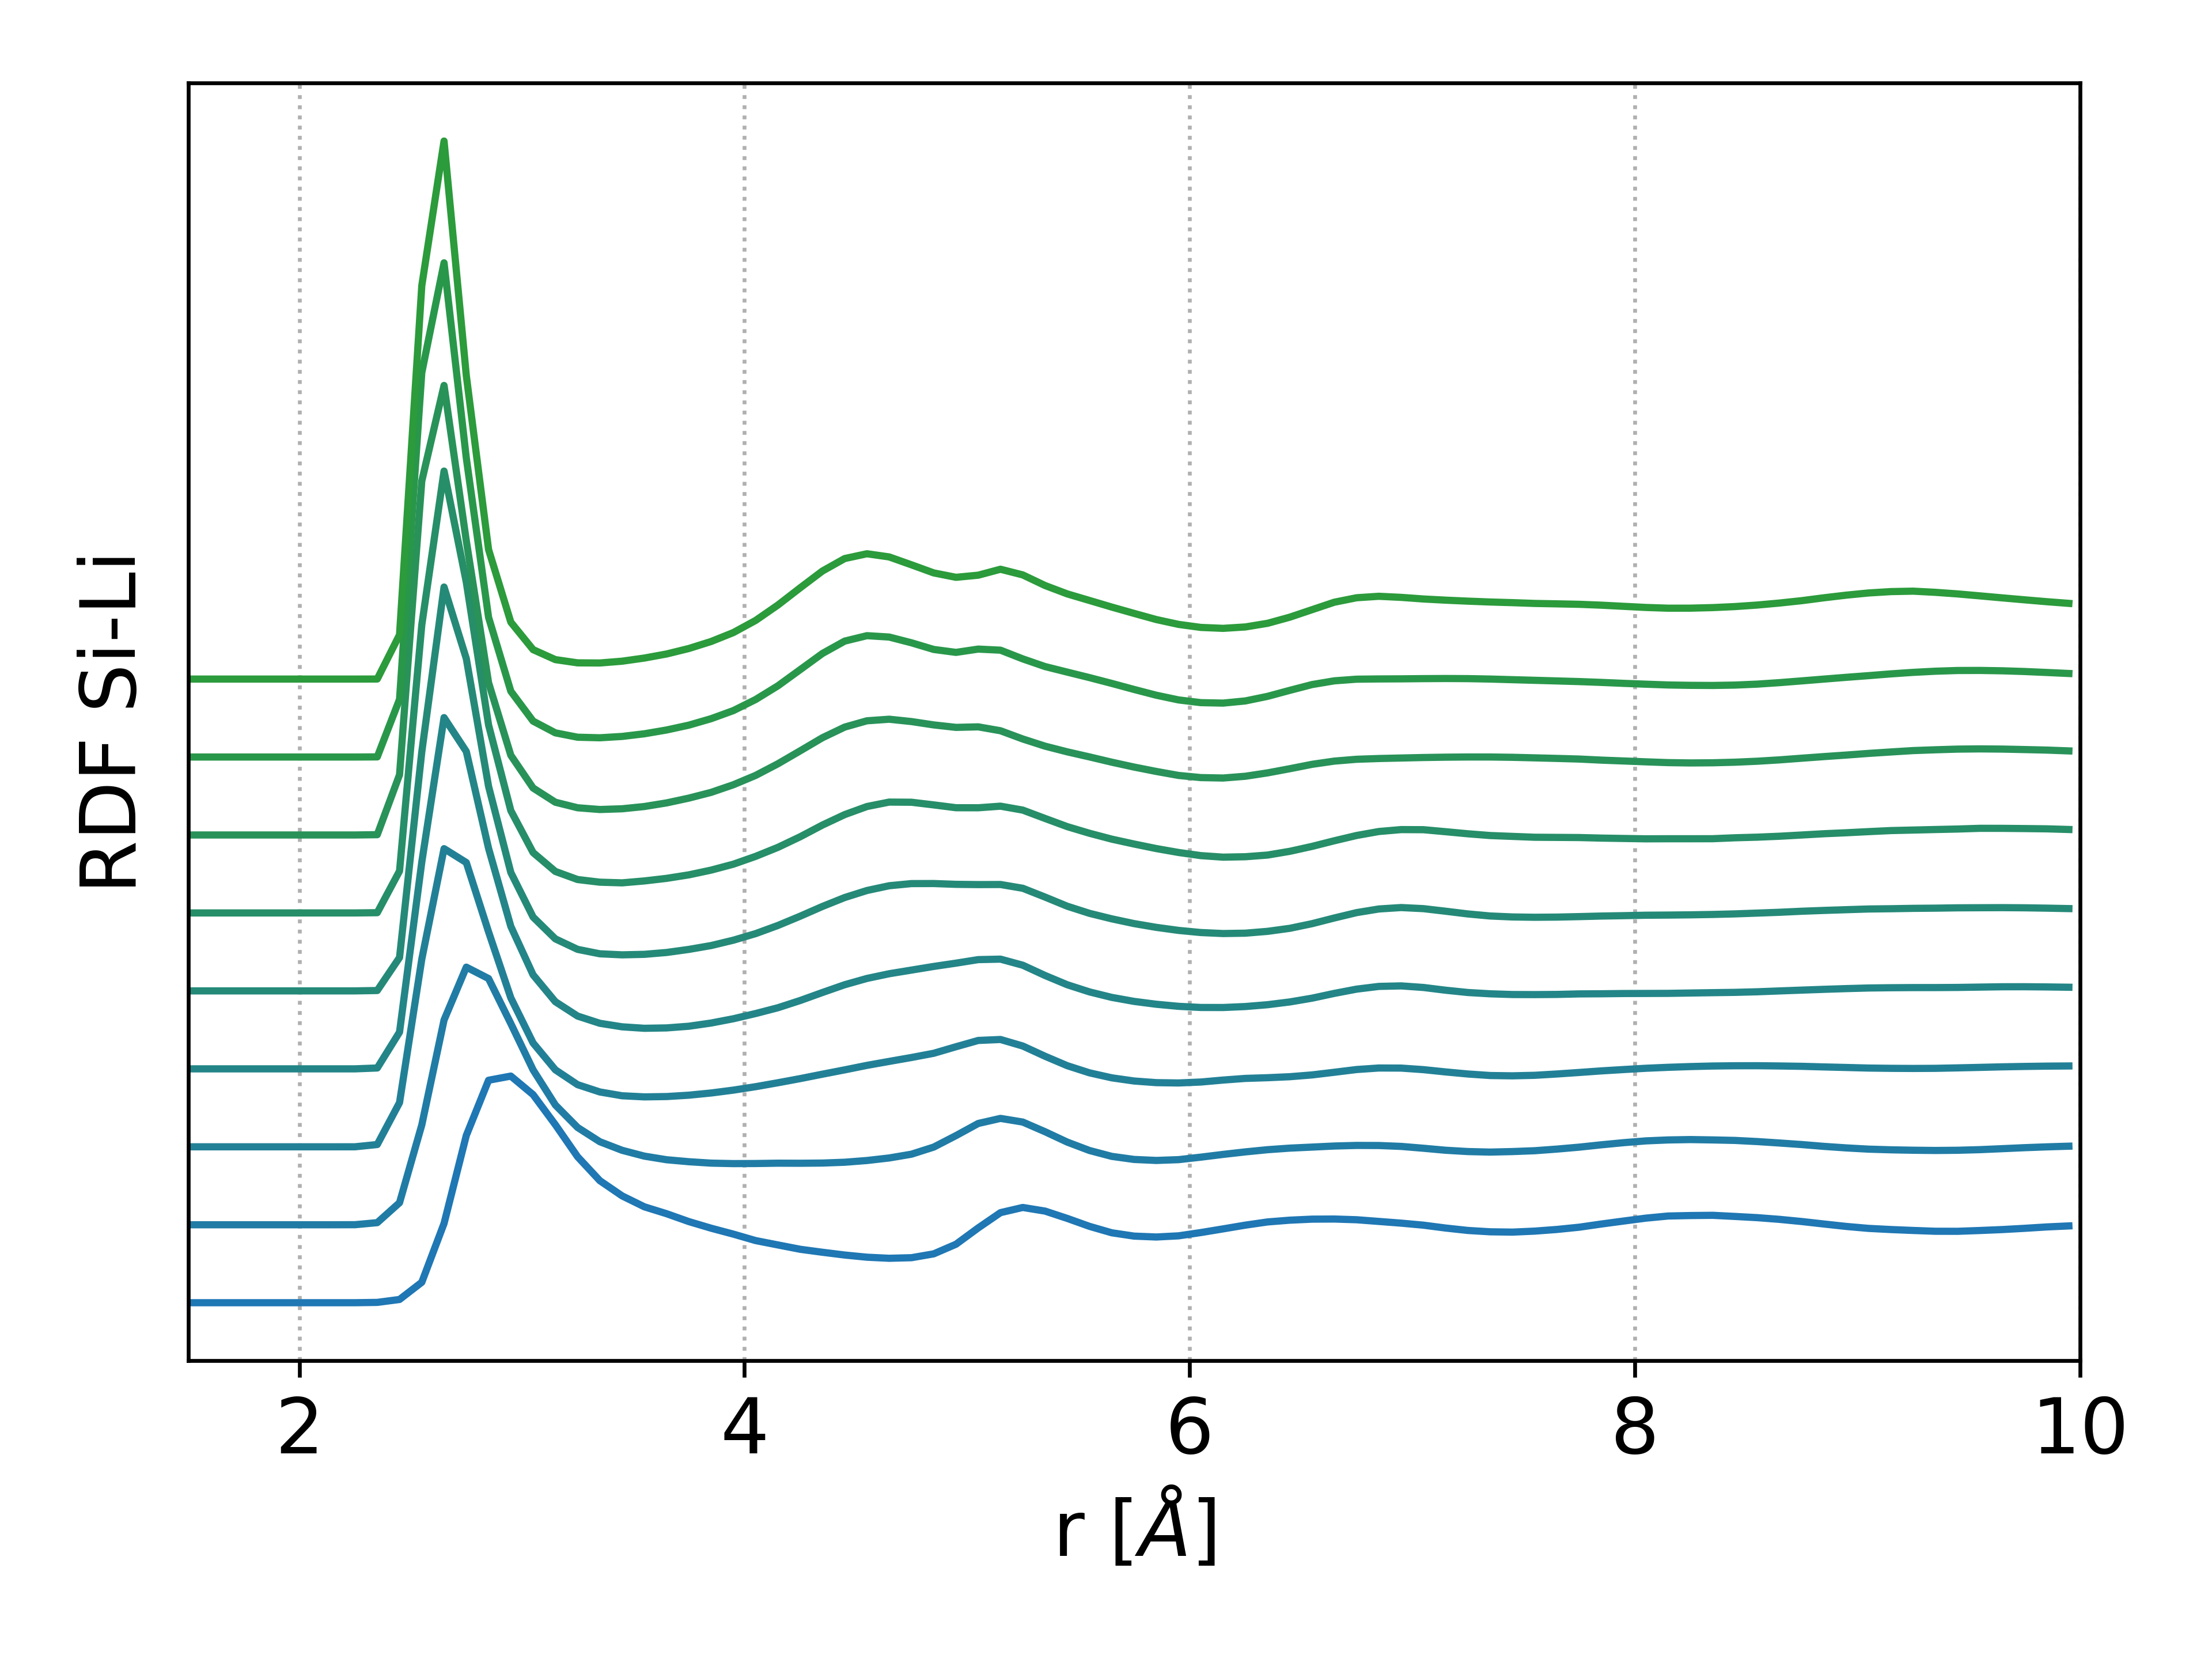
\includegraphics[width=0.8\textwidth]{caracterizacion/rdf-SiLi.png}
    \caption{Distribución radial de a pares para Si-Li de las estructuras 
    minimizadas. Cada curva se corresponde con un valor de concentración 
    distinto.}
    \label{fig:rdf-SiLi}
\end{figure}
Para el primer pico de la RDF$_{Si-Li}$ se ve el comportamiento contrario, el 
centro del mismo se desplaza a distancias menores a medida que la concentración
de litio aumenta. Esto es acompañado con un aumento de la altura del pico y una
disminución de su ancho. Para el segundo pico también se observa un desplazamiento
del mismo hacia distancias menores, pero por encima de $x = 1.71$ el pico se
divide en dos picos con distintas alturas dependiendo de la concentración. Esto
es analizado con mayor detalle en la sección \ref{s:intercionexion}.

\subsection{Número de coordinación}

De la misma manera que se definió la distribuciones radiales de a pares parciales,
se pueden obtener los números de coordinación a un dado tipo de átomos. CN$_{ij}$
se corresponde con la cantidad de átomos vecinos de tipo $j$ para un átomo central 
de tipo $i$ hasta una cierta distancia de corte. Para la elección de dicho valor 
se considera hasta el primer pico de la $g_{ij}(r)$ correspondiente. Debido a que 
en los materiales amorfos la primera y la segunda esfera de coordinación pueden 
llegar a estar superpuestas, el límite superior de integración no está definido 
unívocamente para todas las concentraciones consideradas ~\cite{lamparter1995}.
Para el número de coordinación promedio para átomos de Si vecinos de otros átomos 
de Si se calculó contando el número de dichos vecinos utilizando un radio de 
corte de 3 \AA. Lo mismo se realizó para Li-Li definiendo un radio de corte de 
4 \AA. Para el caso de Si-Li se utilizó el criterio de considerar como radio de 
corte el valor $r$ para el cual la $g(r)$ presenta un mínimo entre los dos picos
a primeros y segundo vecinos. Los resultados se muestran en la figura 
\ref{fig:cn1}.
\begin{figure}[th]
    \centering
    \includegraphics[width=0.8\textwidth]{caracterizacion/cn.png}
    \caption{Promedio del primer número de coordinación en función de la 
    concentración de litio para Li-Li, Si-Si y Si-Li. Como radio de corte se 
    utilizó la distancia posterior al primer pico de la RDF correspondiente. En 
    los casos que no se aprecia la barra de error, es porque la misma es menor 
    que el tamaño de los puntos.}
    \label{fig:cn1}
\end{figure}

Para el caso del CN$_{Si-Si}$, se tiene que esta cantidad decrece de 4 a 2, a 
medida que la concentración de Li aumenta. Esto indica que a valores pequeños de 
$x$ la estructura de Si mantiene sus conexiones tetraédricas, mientras que para
valores grandes de $x$ el Si tiende a formar cadenas periódicas unidimensionales.
El CN de Si-Li y Li-Li presenta valores pequeños para concentraciones bajas y 
aumenta monótonamente hasta alcanzar valores de 10 y 12, respectivamente, que se
asemejan al valor de una estructura de empaquetamiento compacto.

\begin{figure}[th]
    \centering
    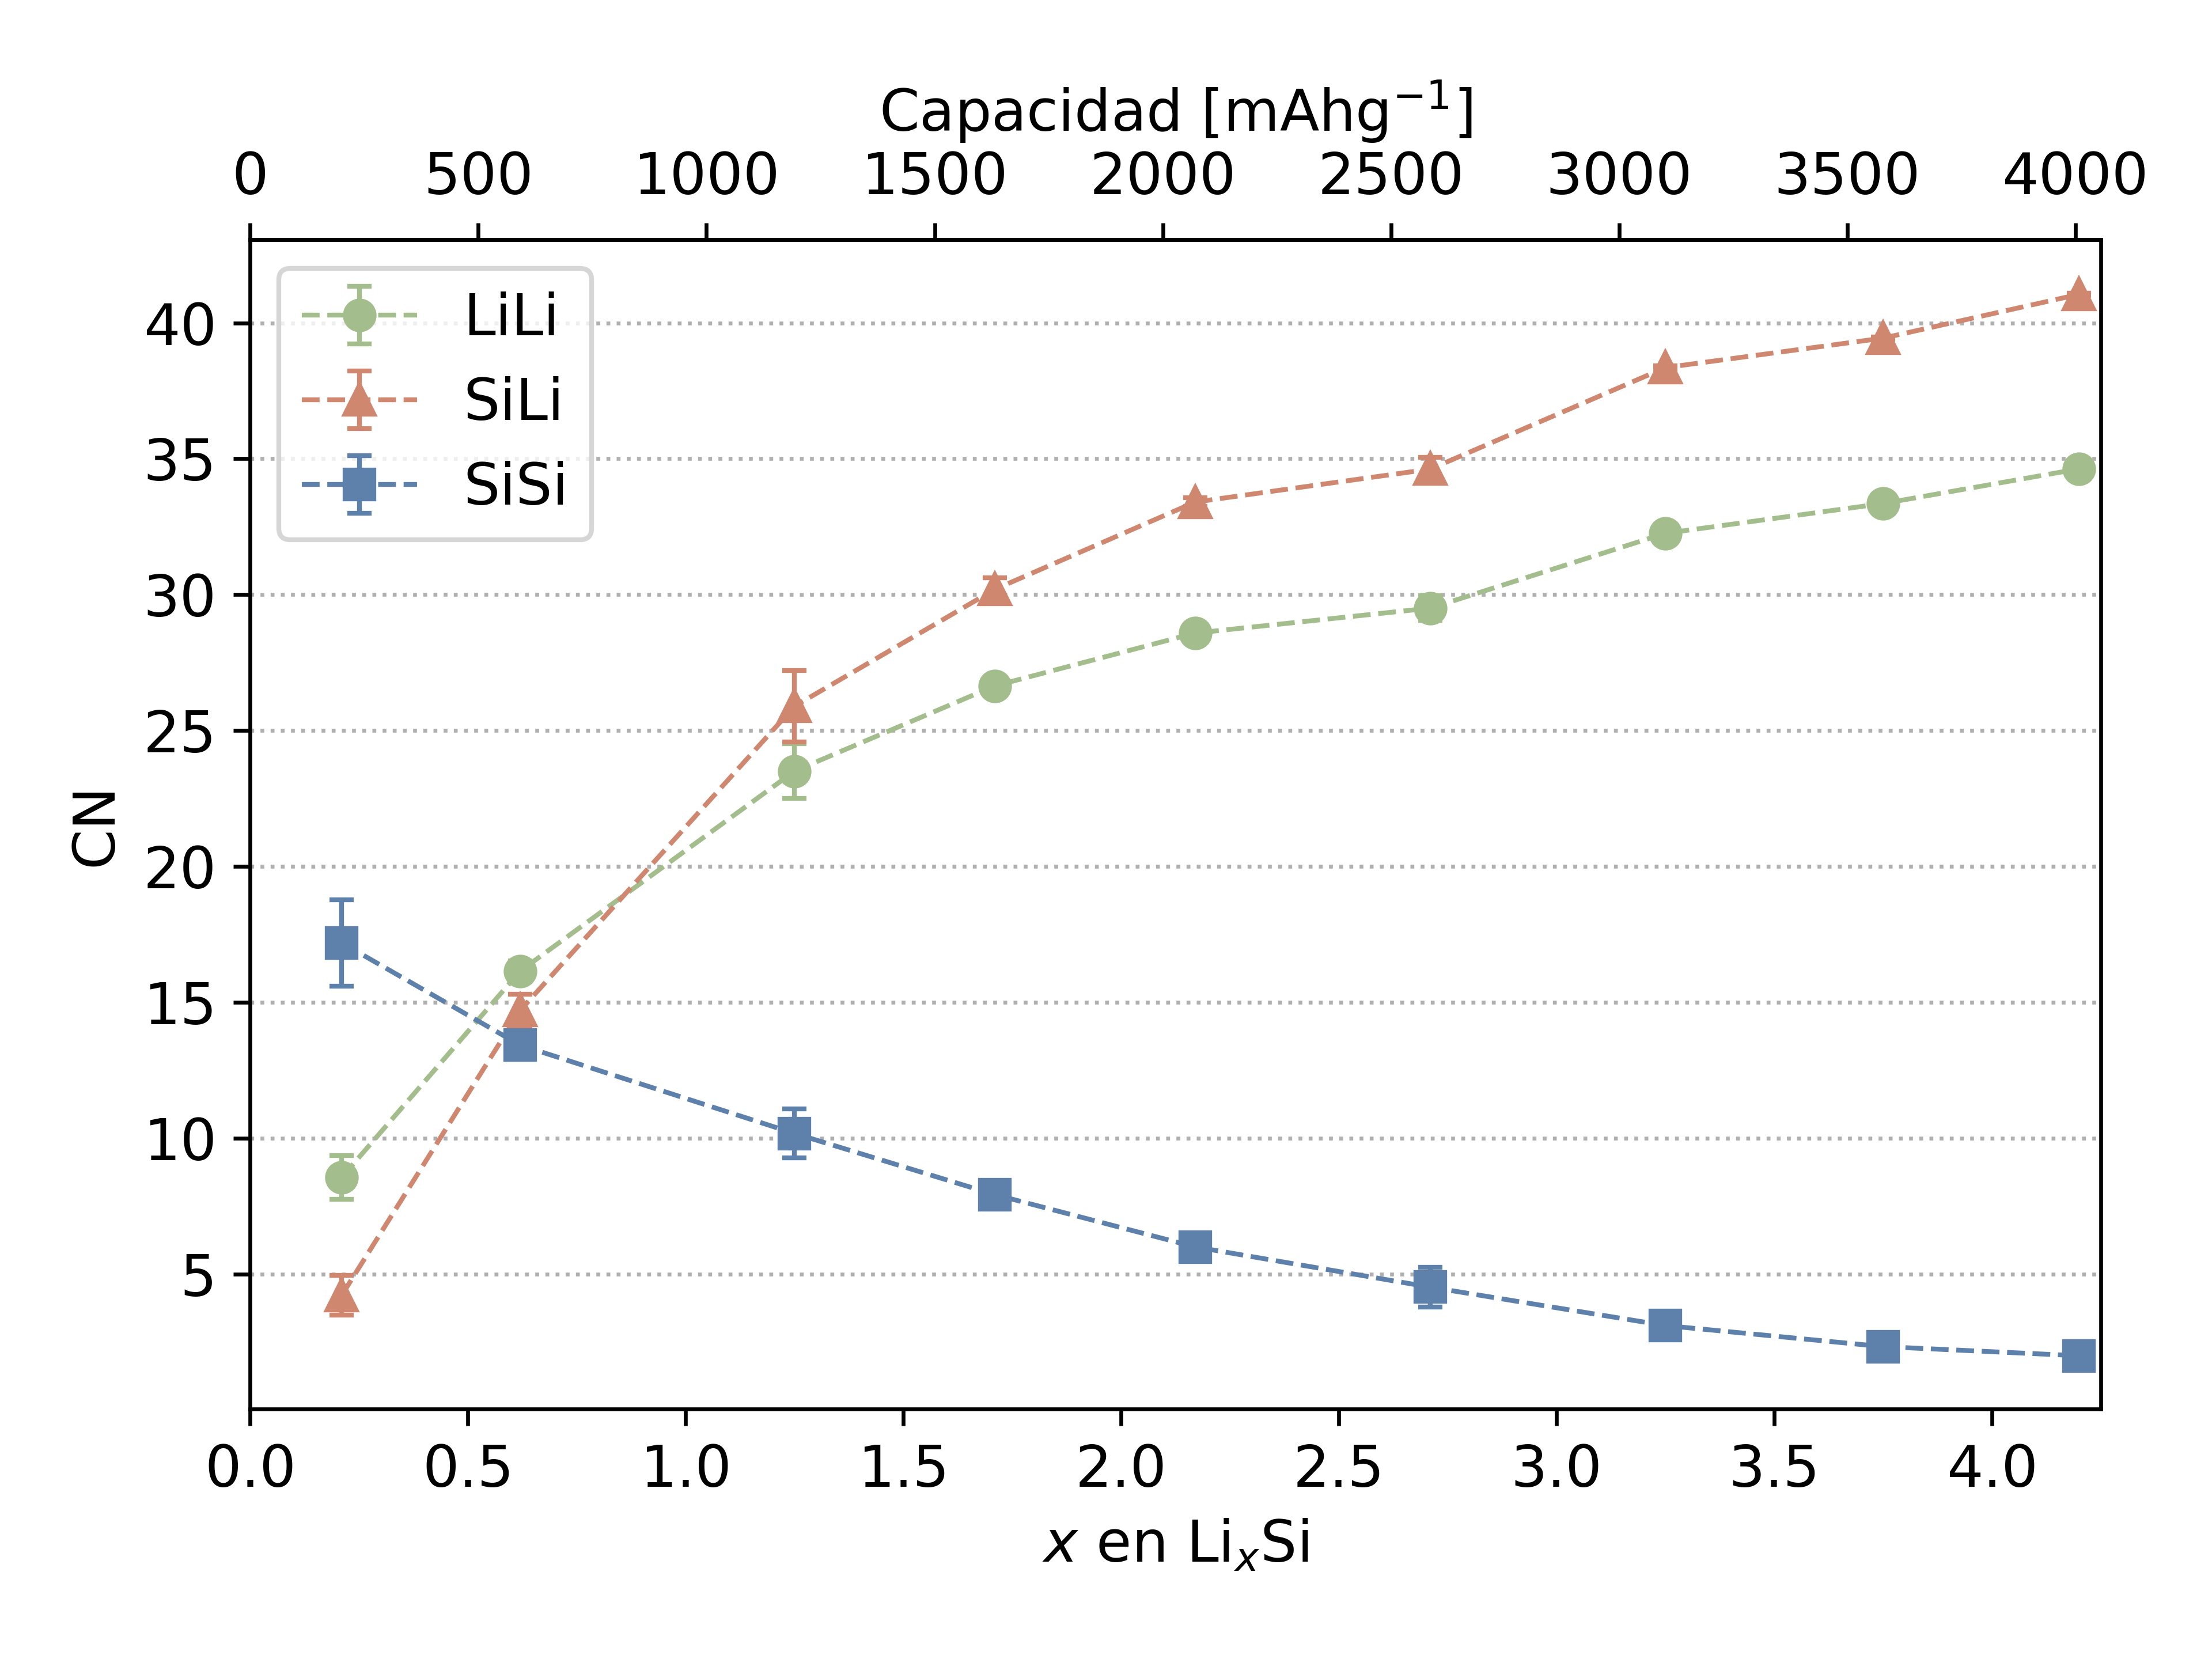
\includegraphics[width=0.8\textwidth]{caracterizacion/cn2.png}
    \caption{Promedio del segundo número de coordinación en función de la 
    concentración de litio para Li-Li, Si-Si y Si-Li. Para la elección de los 
    radios de corte que definen el cascarón en el cual se cuentan los vecinos,
    se consideró el segundo pico de la RDF correspondiente. En los casos que no 
    se aprecia la barra de error, es porque la misma es menor que el tamaño de 
    los puntos.}
    \label{fig:cn2}
\end{figure}
Los resultados para el segundo número de coordinación se presentan en la figura 
\ref{fig:cn1}. Estos resultados se obtuvieron considerando un cascarón con un 
radio de corte interno y otro externo, elegidos de manera tal que incluyan el 
segundo pico de la RDF. La elección de dichos valores varió dependiendo del tipo
de átomos que se consideraron. En todos ellos se tomó como radio de corte interno 
el radio de corte del primero número de coordinación. Luego, para el radio de 
corte externo se utilizaron valores de 5.0 \AA\ para Si-Si y 6.0 \AA\ para Li-Li
y Si-Li.

Para los valores de CN$_{Si-Si}$ se observa un aumenta para concentraciones bajas
de Li si se lo compara con el CN de primeros vecinos. Para valores mayores de $x$,
se puede ver como el valor de CN también tiende a 2, lo cual es coherente con la
formación de cadenas que se notó previamente. La tendencia cualitativa del segundo
CN para Li-Li y Si-Li es la misma a la observada en el primer CN, sólo que ahora
empieza en un valor cercano a 5 y tiende a 35 y 40, respectivamente. Este valor 
es mucho mayor que el que se tiene para los segundos vecinos en una estructura 
de empaquetamiento compacto, que es 6 para la estructura cristalina FCC. Incluso 
es mayor a la suma del segundo (6) y del tercer vecino (24) esperado para la red 
FCC.

\subsection{Formación de clusters}

Del gráfico a: This is defined as the percentage of Si atoms that lay at at 
distance from other Si atom larger that $r_{cut}$. When the cutoff radius is 
higher that the distance at which the first peak of the RDF$_{Si-Si}$ finishes, 
there are no isolated Si atoms, rather an a-Si network where all atoms are 
interconnected.

Del gráfico b: When the cutoff radius is lower than the first RDF$_{Si-Si}$ peak, 
the number of clusters is equal to the number of Si atoms, and when the cutoff 
radius is larger than the first RDF$_{Si-Si}$ peak, there is only one cluster.

\begin{figure}[h]
    \centering
    \begin{subfigure}{.475\textwidth}
        \centering
        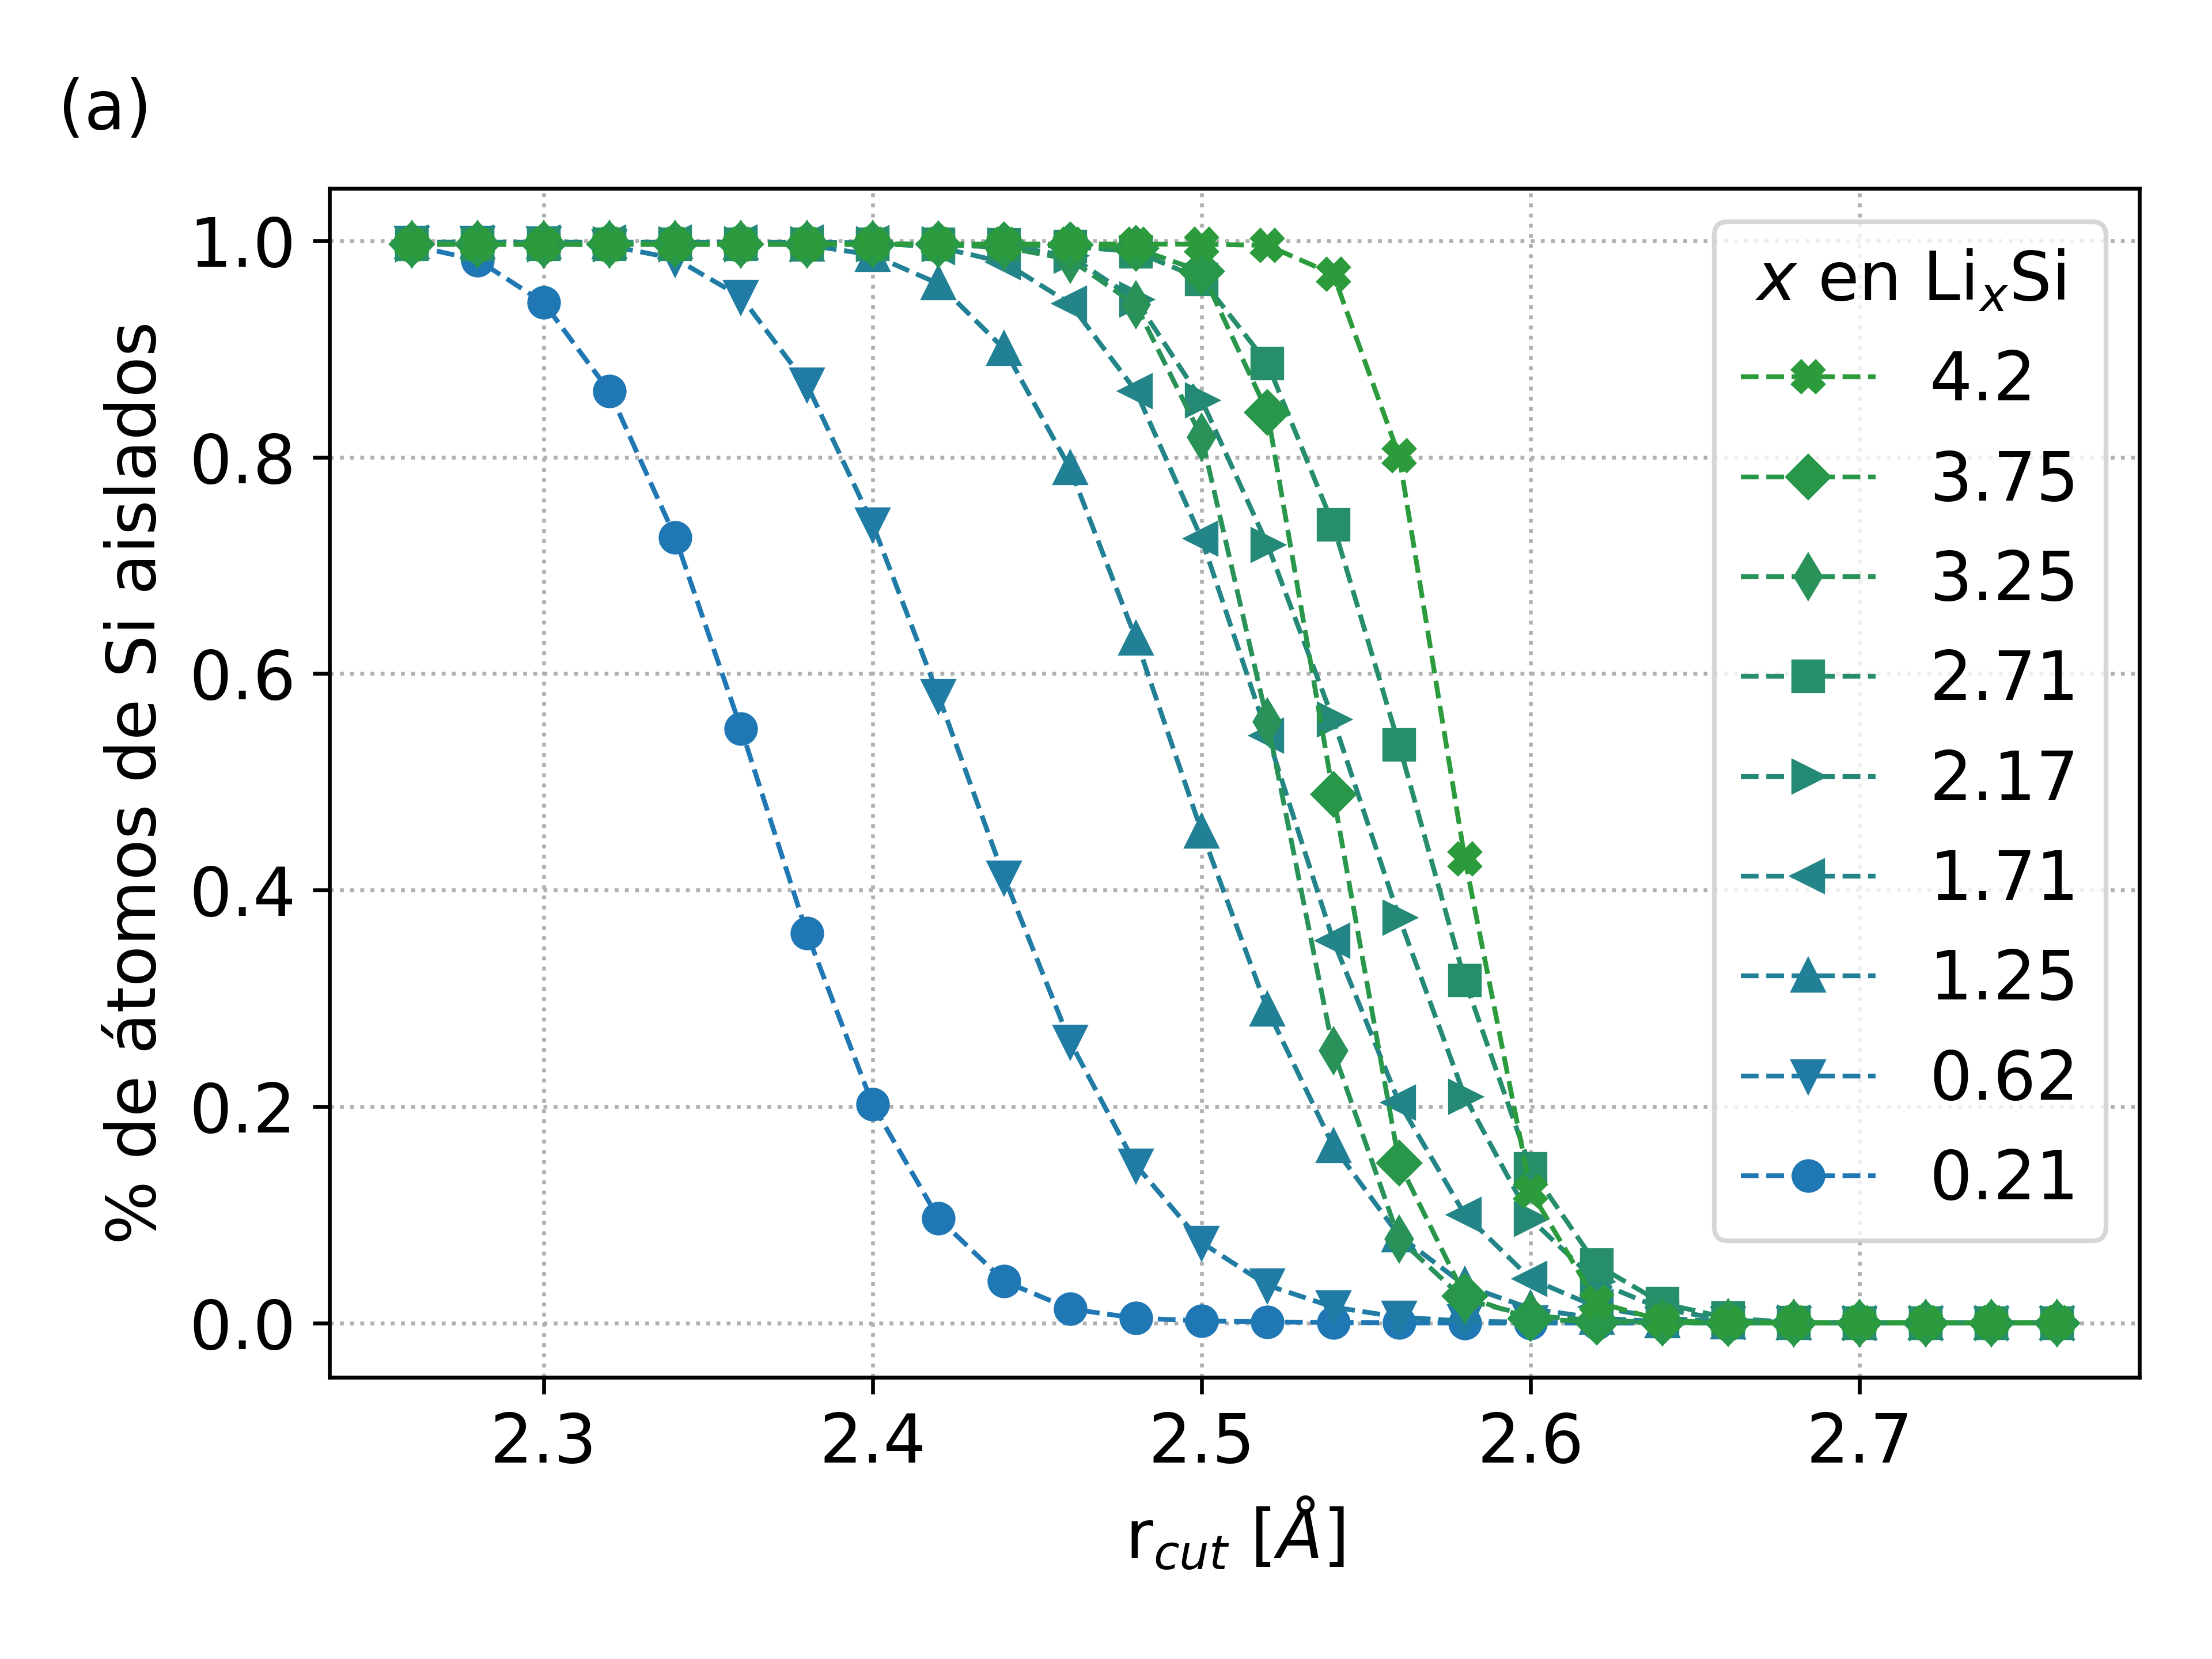
\includegraphics[width=\textwidth]{caracterizacion/cluster-isolated.png}
        \caption{Porcentaje de átomos de Si aislados en función de la elección del
        radio de corte.}
        \label{fig:clusters-isolated}
    \end{subfigure}
    \hfill
    \begin{subfigure}{.475\textwidth}
        \centering
        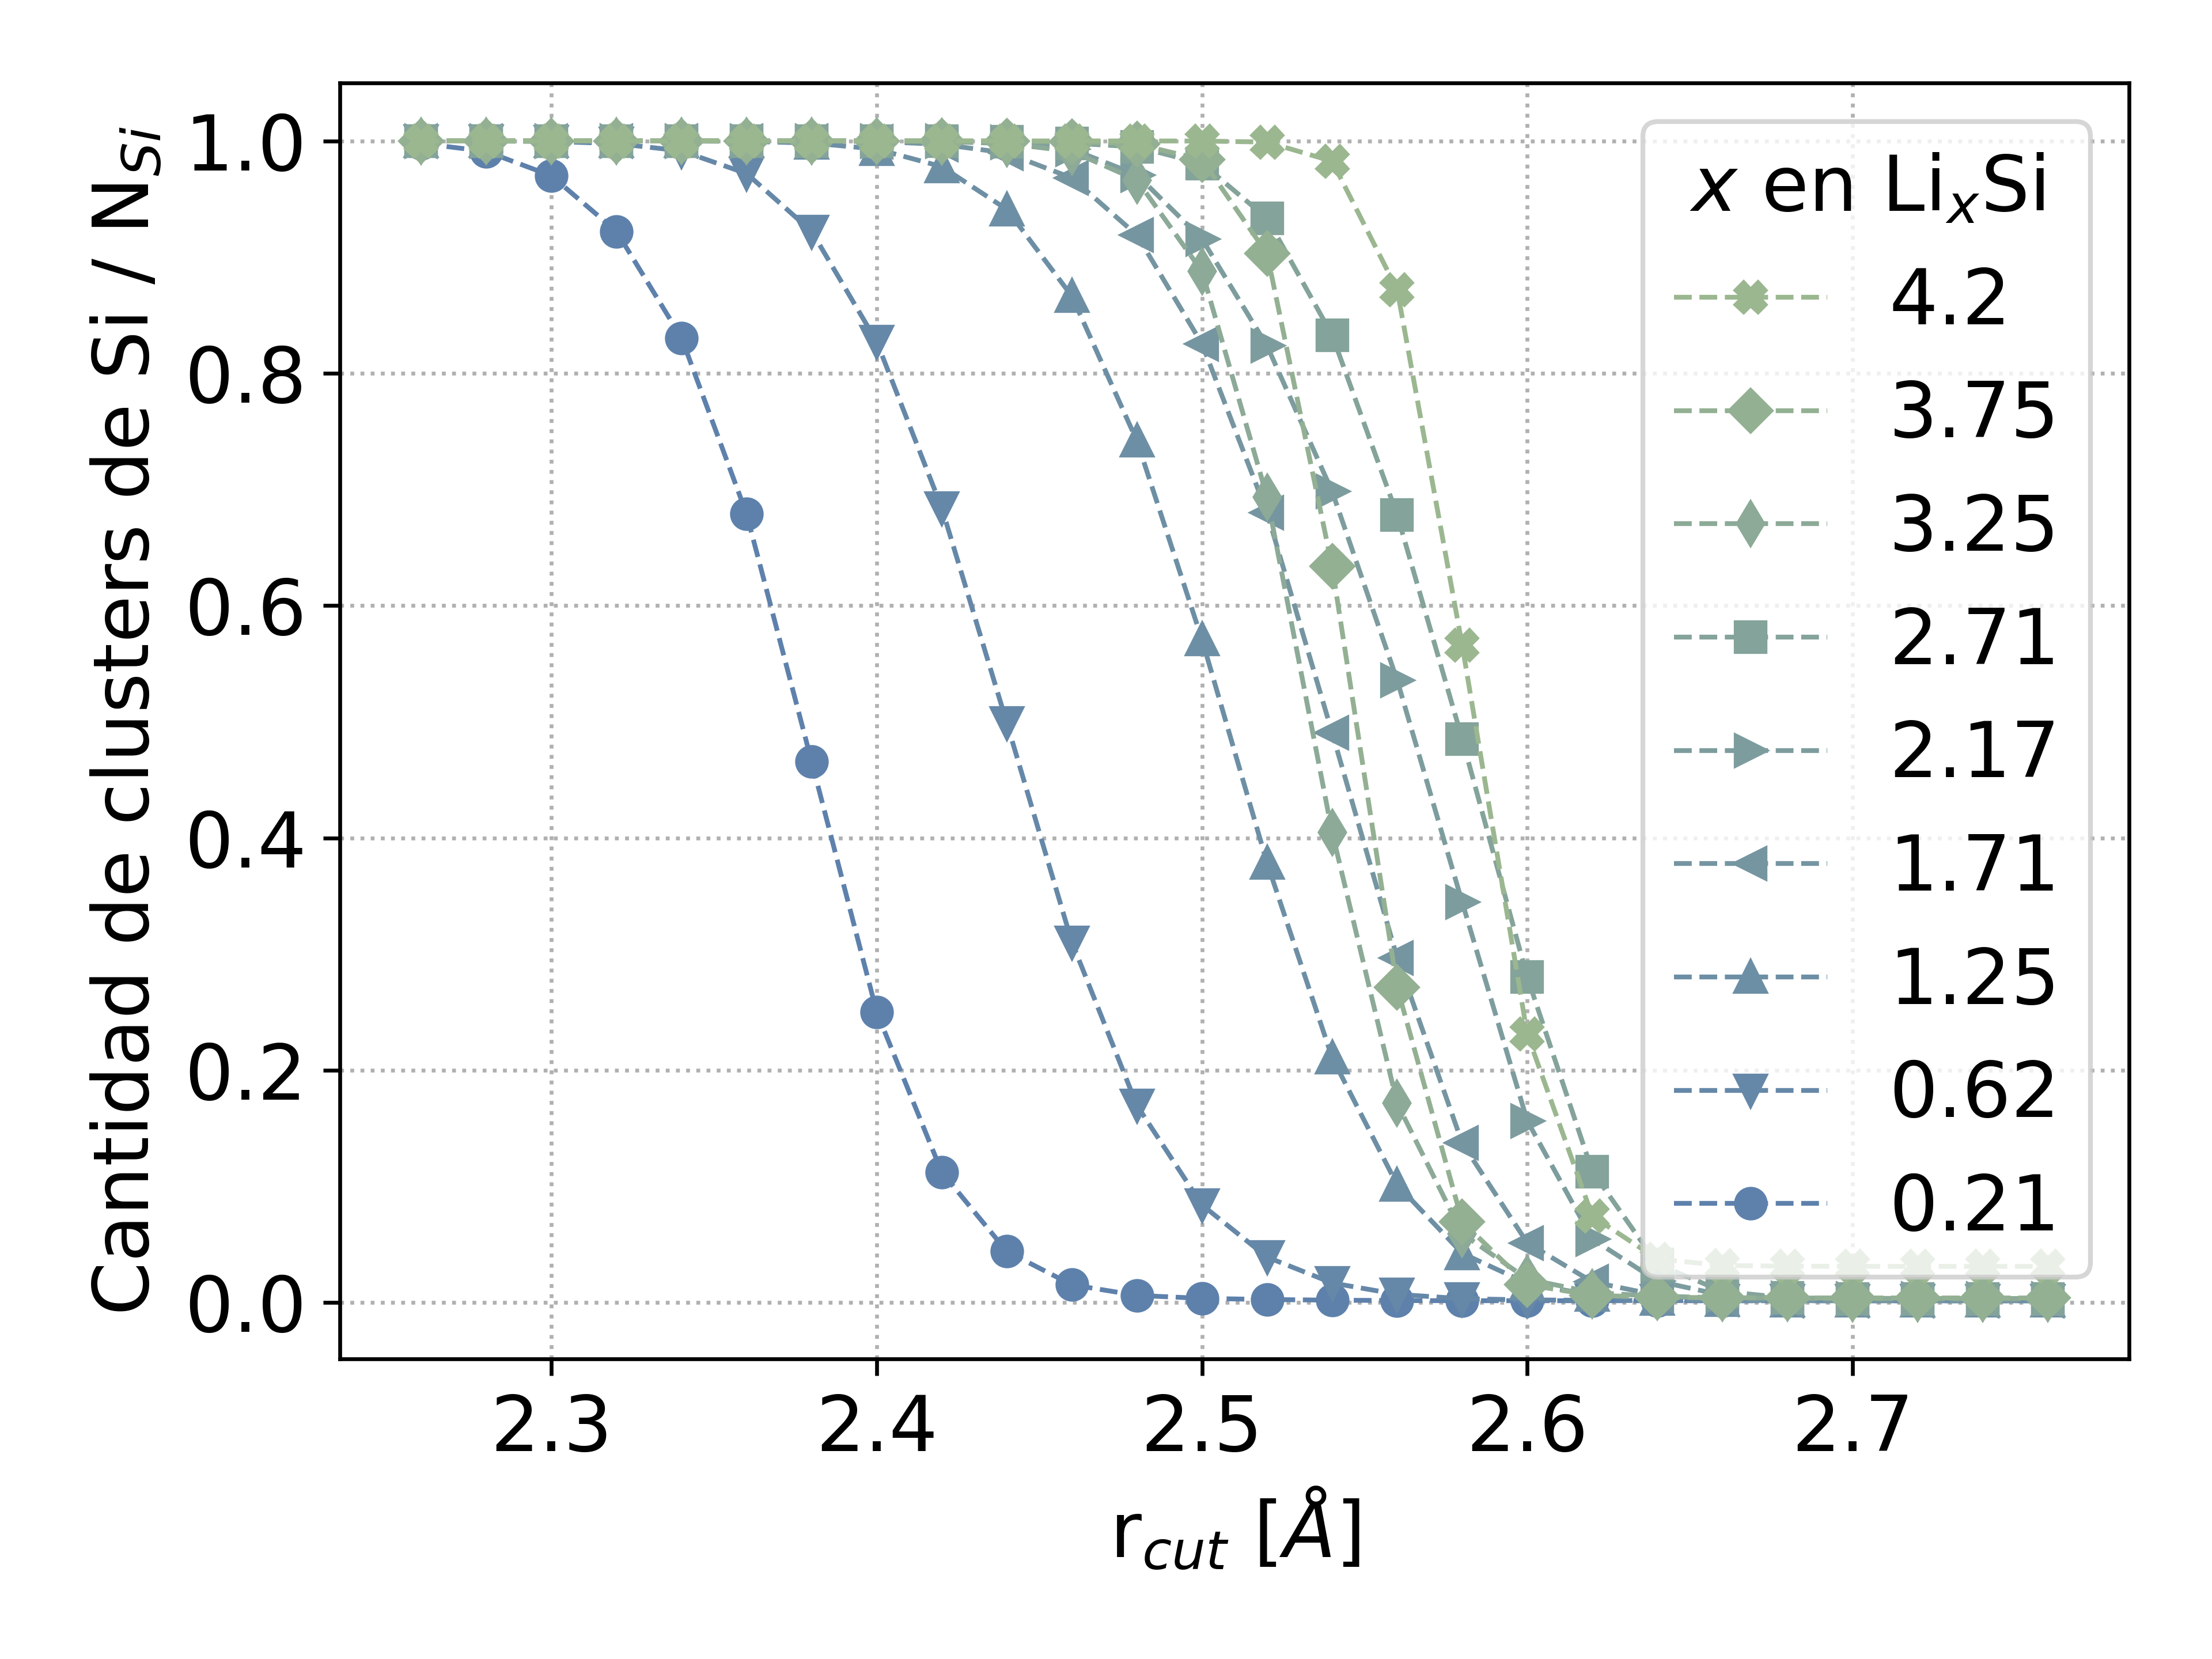
\includegraphics[width=\textwidth]{caracterizacion/cluster-nclusters.png}
        \caption{Número de clusters de Si sobre el número total de átomos de Si.}
        \label{fig:clusters-nclusters}
    \end{subfigure}
    \caption{Formación de clusters indicando una red amorfa de silicio.}
    \label{fig:clusters}
\end{figure}

\subsection{Interconexión de clusters}\label{s:intercionexion}

\subsection{Ordenamiento a corto alcance}

Acá primero el texto...
\begin{figure}[th]
    \centering
    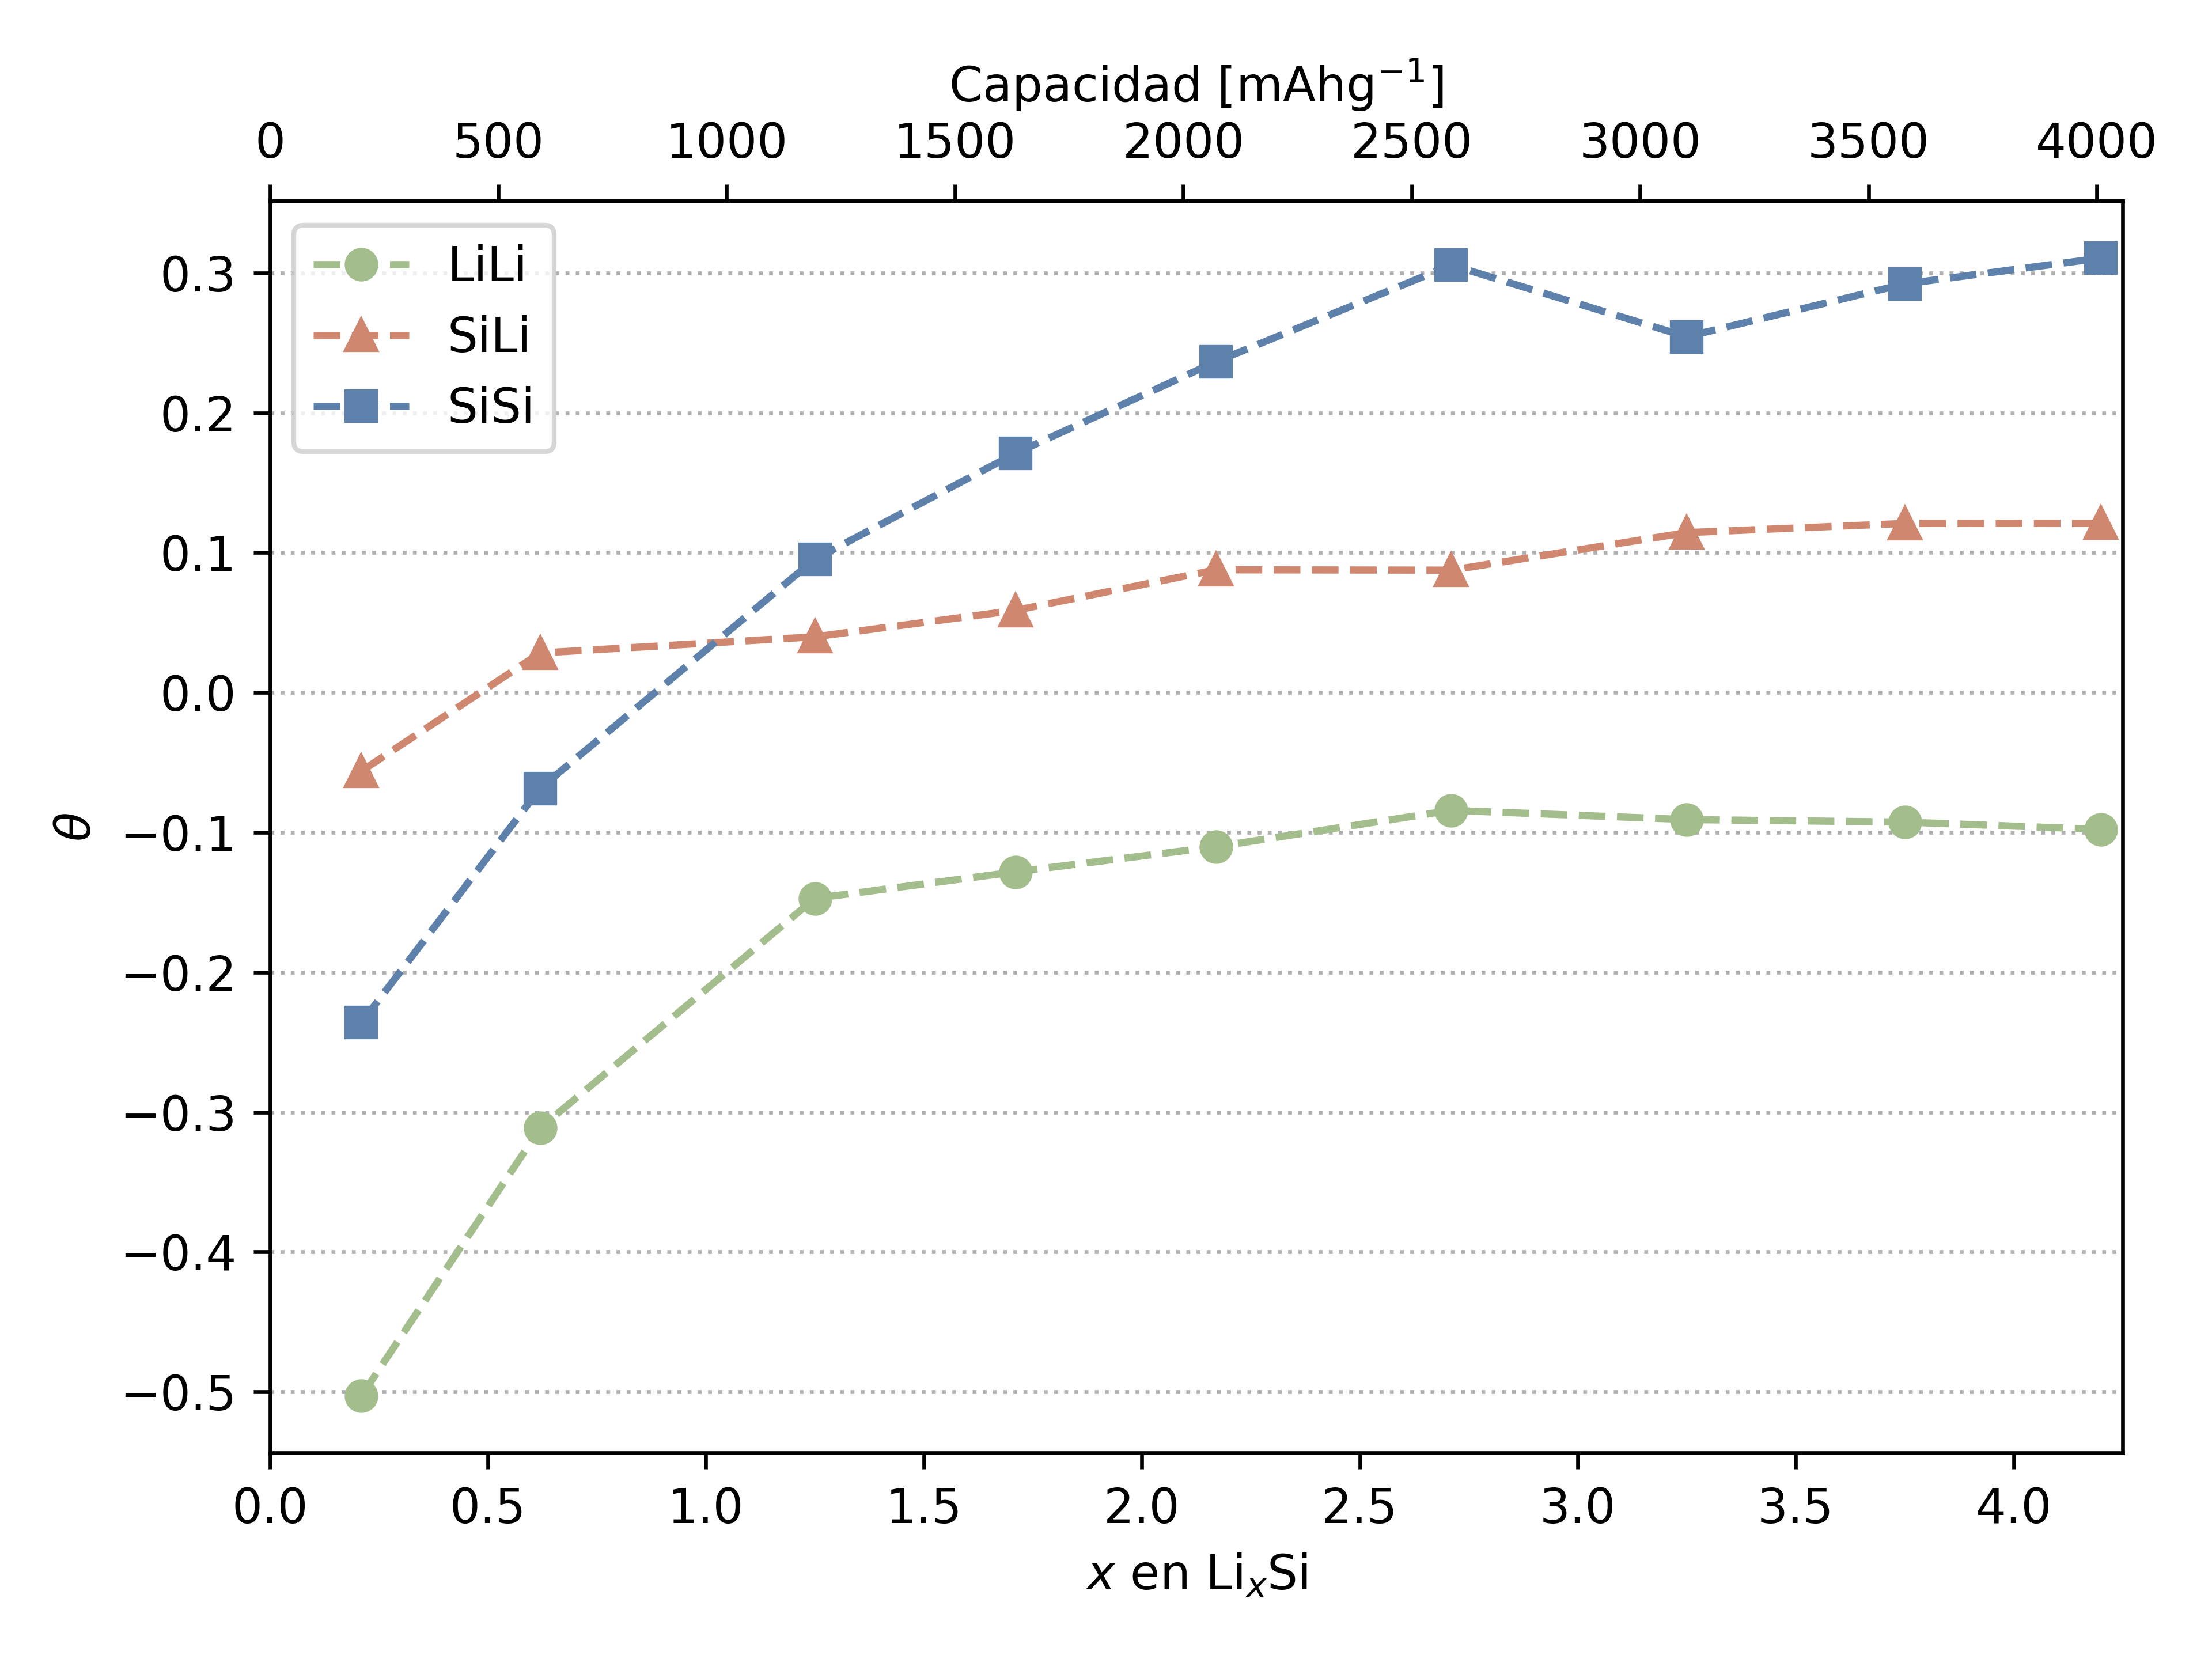
\includegraphics[width=0.8\textwidth]{caracterizacion/sro.png}
    \caption{Parámetros $\theta_{Li-Li}$, $\theta_{Si-Li}$ y $\theta_{Si-Si}$ 
    en función de la concentración de Li. El primer subíndice indica el tipo de
    átomo que se considera como central mientras que el segundo es el vecino. El
    radio de corte se eligió luego del primer pico de la RDF correspondiente.}
    \label{fig:sro}
\end{figure}


\section{Conclusiones del capítulo}


% \chapter{Modelo funcional de densidad de enlace estrecho para aleaciones de Li-Si}\label{ch:modelo}
\thispagestyle{empty}

\vspace{50pt}

\begin{adjustwidth}{50pt}{50pt}
    Resumen...
\end{adjustwidth}

\clearpage
\newpage
\thispagestyle{empty}
\mbox{}
\newpage


% \subsection{Predicción del tamaño óptimo de partícula}

Como ya ha sido mencionado a lo largo de esta tesis, el criterio de carga rápida
está definido por la obtención del 80\% de la capacidad del electrodo en 15 
minutos, lo cual se traduce en un SOC$_{\max}$ de 0.8 y una C-rate de 4 C. La
Figura \ref{fig:prediccion} muestra donde se encuentra cada sistema analizado en
el diagrama $\log(\Xi)$--$\log(\ell)$ para dicha C-rate. También se presenta una
curva de nivel con una línea roja correspondiente a SOC$_{\max} = 0.8$. Puede
observarse que tres de los materiales ya se encuentran en la región de 
SOC$_{\max}$ mayor a 0.8 (LCO, LMNO y LNMO), mientras que los otros se encuentran
por debajo de este valor (LTO, Grafito amorfo y LFP).
\begin{figure}[h!]
    \centering
    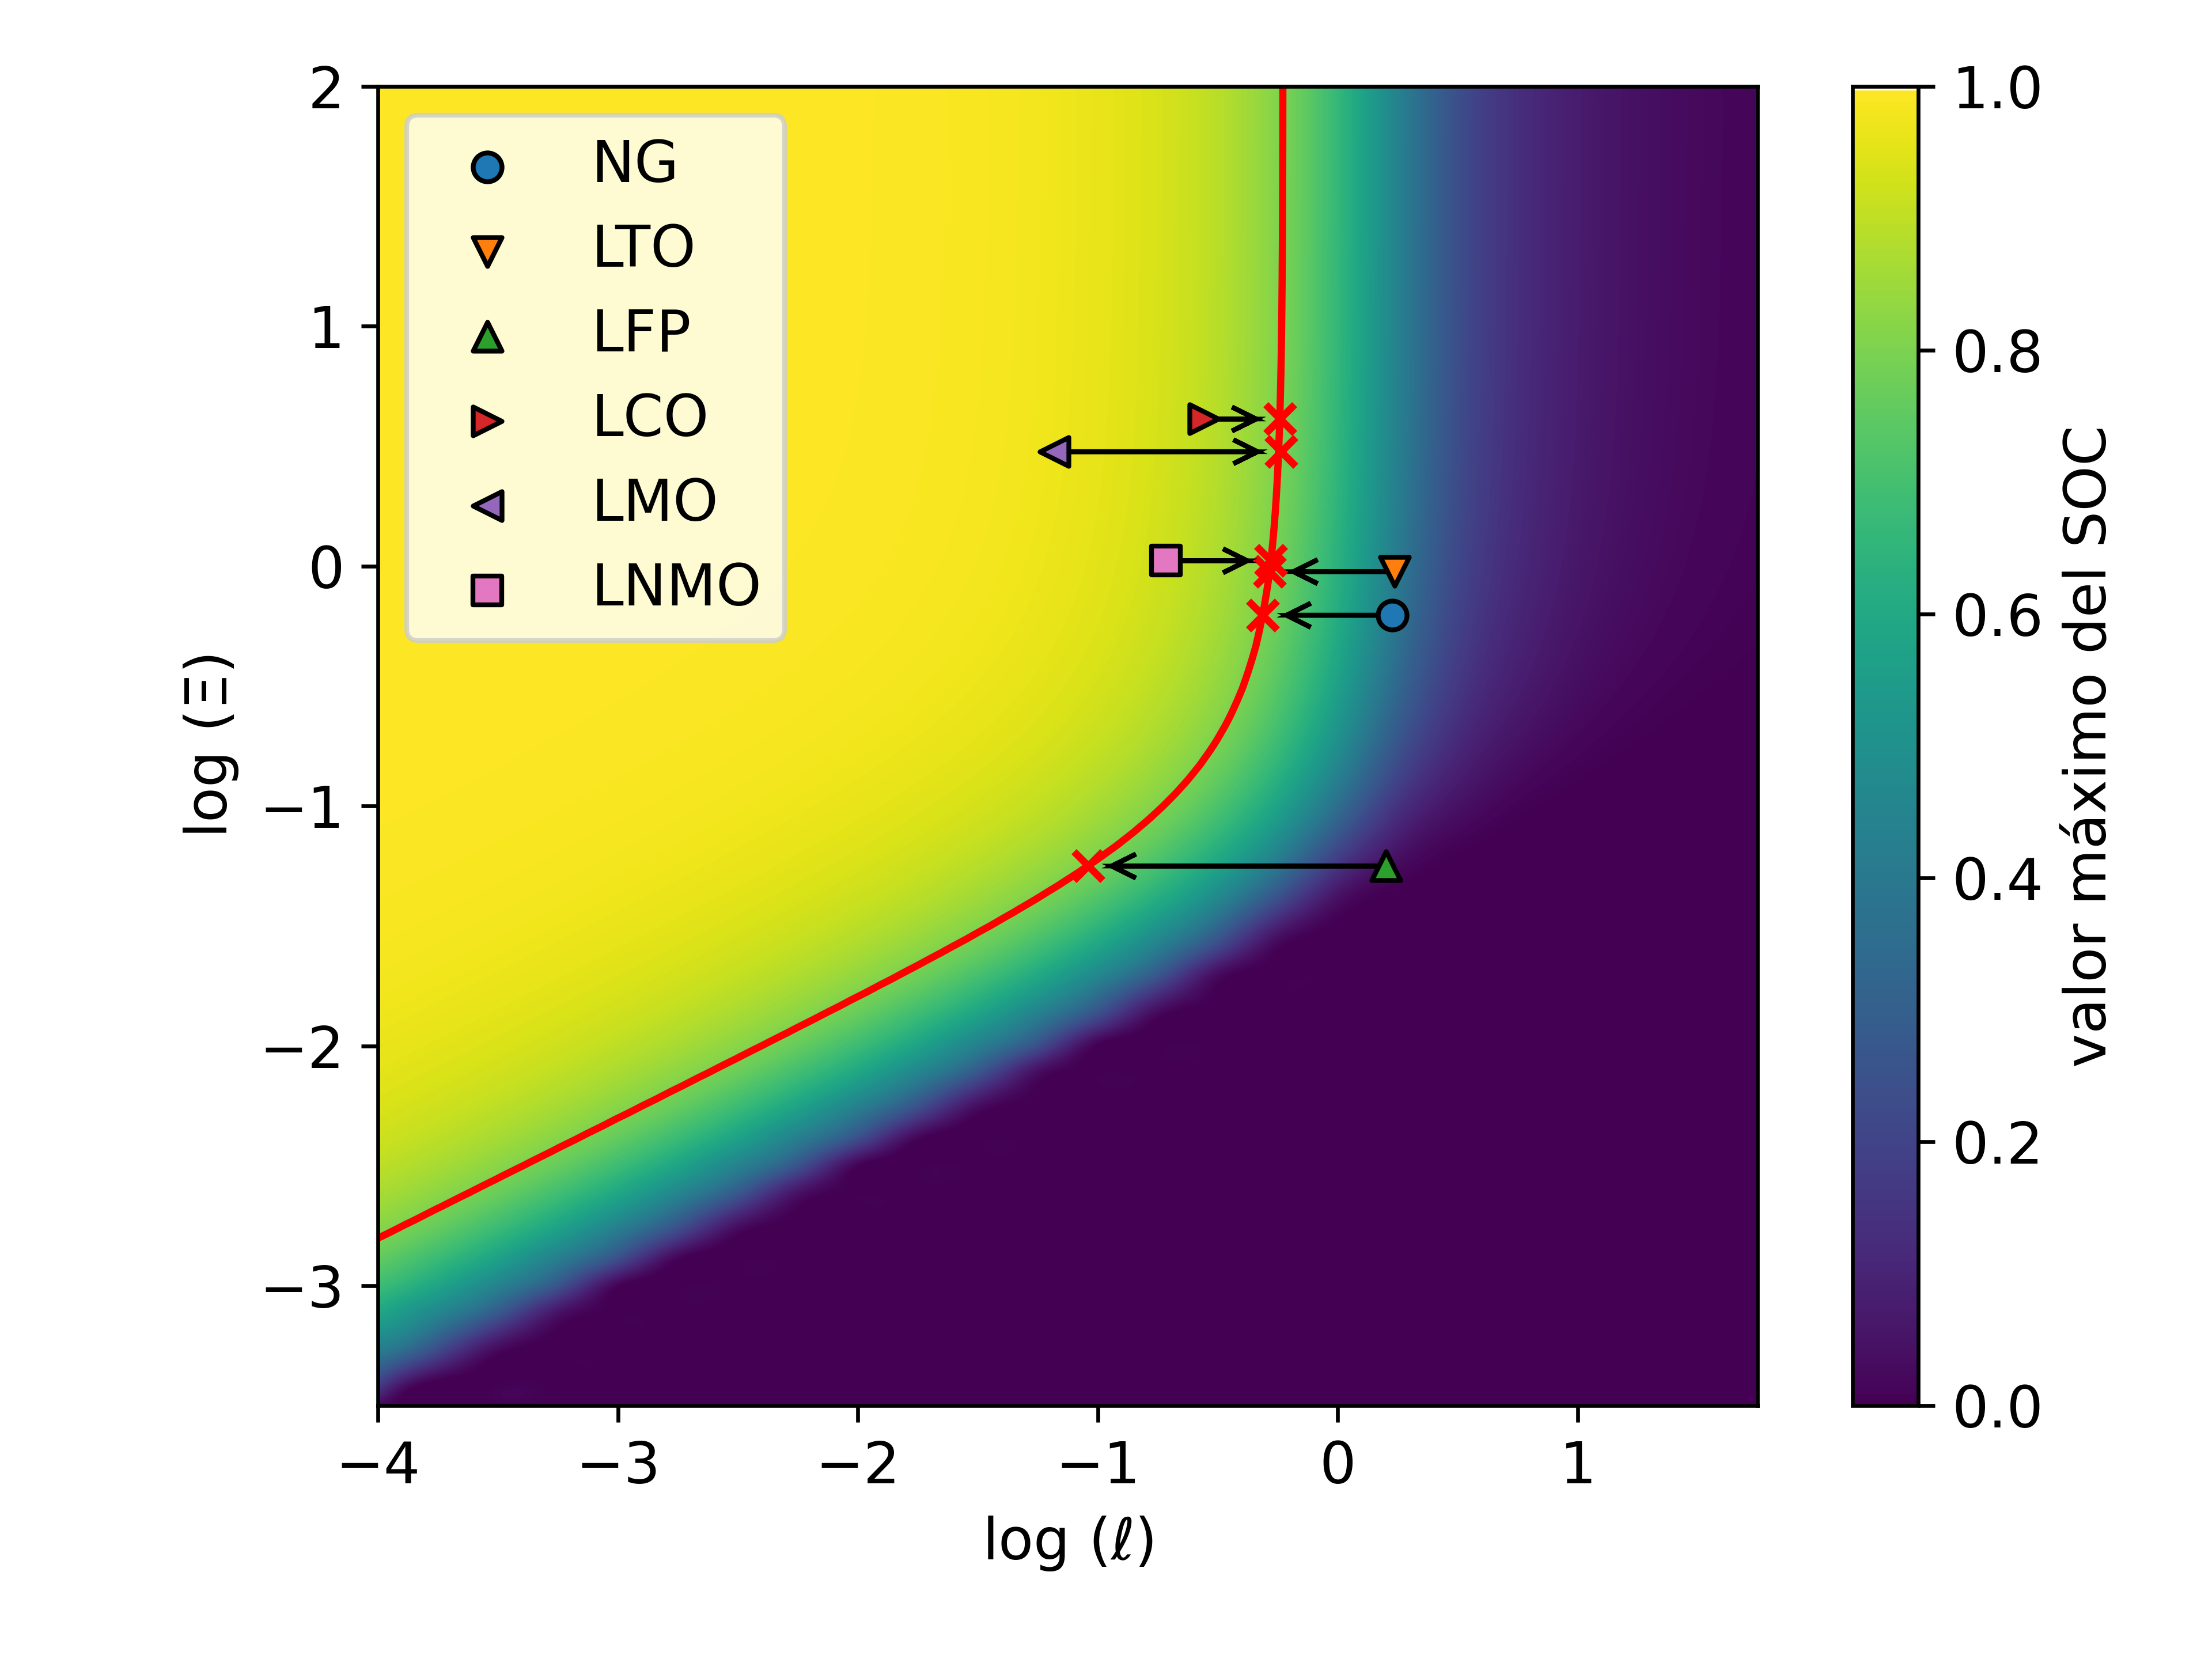
\includegraphics[width=0.7\textwidth]{FastCharging/un/resultados/prediccion/prediccion.png}
    \caption{Diagrama de SOC$_{\max}$ mostrando la ubicación de los materiales 
    usuales de LIBs a 4 C para las referencias consideradas \cite{mancini2022,
    he2012, lei2015, wang2019high, bak2011, nishikawa2017}. En los casos en los 
    que la curva de cargado a 4 C no estaba disponible, el valor del punto fue 
    predicho con el modelo. La línea roja muestra la curva de nivel 
    correspondiente al valor 0.8 de SOC$_{\max}$. Las flechas muestran el cambio
    en el tamaño de la partícula que debería efectuarse para obtener dicho valor
    a la C-rate dada. Las curces sobre la línea muestran la posición de estos
    tamaños de partícula nuevos.}
    \label{fig:prediccion}
\end{figure}
Haciendo uso del diagrama se puede predecir una forma simple y rápida el tamaño 
de partícula requerido para satisfacer el criterio de carga rápida. Dado que los
valores de $D$ y $k^0$ ya fueron ajustados, el valor de $d$ seleccionado por el
experimento y el de C-rate por el criterio, el valor de $\Xi$ es constante. Luego,
para alcanzar el valor de 0.8 de SOC$_{\max}$ hay que variar $\ell$ y esto se
logra disminuyendo o aumentando el tamaño de la partícula, según sea necesario. 
Este desplazamiento necesario está representado por las flechas en la Figura 
\ref{fig:prediccion} para cada caso. Ya se ha apreciado que tres sistemas se 
encuentran en la región ya optimizada (LCO, LMO y LNMO), por lo que en estos casos
los tamaños predichos para alcanzar SOC$_{\max} = 0.8$ a 4 C serán mayores que 
los experimentales. Por el contrario, el resto de los materiales (LTO, Grafito
amorfo y LFP) tienen que ser mejorados con una reducción del tamaño de partícula
para cumplir la condición. En la tabla \ref{t:prediccion} se muestran los tamaños
de partícula predichos para todos los materiales en la tercera columna para este
criterio. Las incertidumbres se determinaron por propagación de errores con 
derivadas parciales. Ya que el tamaño de la partícula sólo aparece en el parámetro
$\ell$, al definir $\ell_{\text{opt}}$ como el valor al cual el SOC$_{\max}$ 
alcanza el valor deseado de 0.8 y usar que $V/A = d/z$ se puede despejar de la 
ecuación \ref{eq:ele} que
\begin{equation}
    d = \sqrt{\frac{t_h z D 10^{\ell_{\text{opt}}}}{C_r}}.
\end{equation}
Si además se supone que toda la incertidumbre está asociada al coeficiente de 
difusión $D$, al cual ya se le calculó su incerteza, se puede obtener que
\begin{equation}
    \Delta d = \frac{1}{2} \sqrt{\frac{t_h z 10^{\ell_{\text{opt}}}}{C_r D}} \Delta D.
\end{equation}

\begin{table}[h!]
    \centering
    \caption{Tamaño experimental y valores predichos para cargar el 80\% del
    electrodo en 15 y 5 minutos.} 
    \setlength\extrarowheight{2pt}\stackon{%
    \begin{tabular}{l c c c}
        \toprule
        \textbf{Material del} &
        \textbf{Tamaño} &  
        \textbf{Tamaño predicho} & 
        \textbf{Tamaño predicho} \\
        \textbf{electrodo} & 
        \textbf{experimental [$\mu$m]} &  
        \textbf{para 15 minutos [$\mu$m]} & 
        \textbf{para 5 minutos [$\mu$m]} \\
        \midrule
        Grafito amorfo & 7.5 & 4.027 $\pm$ 0.002 & 2.167 $\pm$ 0.001 \\
        LTO & 1.75 & 0.962 $\pm$ 0.004 & 0.530 $\pm$ 0.002 \\
        LFP & 0.35 & 0.084 $\pm$ 0.002 & 0.0309 $\pm$ 0.0006 \\
        LCO & 20 & 28.8 $\pm$ 0.6 & 16.4 $\pm$ 0.4 \\
        LMO & 0.025 & 0.0734 $\pm$ 0.0003 & 0.0418 $\pm$ 0.0002 \\
        LNMO & 7.999 & 13 $\pm$ 2 & 7.3 $\pm$ 0.8 \\
        \bottomrule
    \end{tabular}
    }{}
    \label{t:prediccion}
\end{table}

Al observarse un buen desempeño para la carga de 15 minutos, se puede exigir un 
poco más que este criterio y predecir el tamaño de partícula requerido para una
C-rate más alta, digamos 80\% de la carga en 5 minutos (12 C). Si bien esta figura
puede parecer sobredemandante a primera vista, reportes recientes consideran 
protocolos de carga de 10 minutos \cite{mattis2021, attia2020}. Los resultados
se muestran en la última columna de la Tabla \ref{t:prediccion}. Como puede 
observarse, el comportamiento depende del sistema y del experimento en particular
considerado. El único caso donde se cumple este último criterio de carga rápida 
es el LMO, ya que el tamaño experimental sobrecumple el criterio. Aunque el LCO 
y el LNMO no cumplen con este último criterio, los cambios en sus tamaños serían
menores, por lo que estos materiales requieren mejoras menores. En el resto de 
los casos, para el LFP se necesitaría una disminución de un orden de magnitud 
en su tamaño, mientras que para el grafito amorfo o el LTO se requeriría una
disminución de su tamaño en un factor de 3.


% % Copyright (c) 2024, Francisco Fernandez
% License: CC BY-SA 4.0
%   https://github.com/fernandezfran/thesis/blob/main/LICENSE
\chapter{Análisis preliminar del comportamiento difusional del litio en el silicio}\label{ch:comportamiento}
\thispagestyle{empty}

\vspace{50pt}

\begin{adjustwidth}{50pt}{50pt}
    Resumen...
\end{adjustwidth}

\clearpage
\newpage
\thispagestyle{empty}
\mbox{}
\newpage

\section{Introducción}


\section{Resultados}

\section{Introducción}


\subsection{Comportamiento electroquímico}

\subsubsection{Cambio de volumen fraccionario}

El cambio de volumen fraccionario puede definirse utilizando una normalización 
relativa al número de átomos de Si en la estructura de acuerdo a
\begin{equation}\label{eq:fvc}
    \text{fvc} = \frac{N_{\text{Si}}}{V_{\text{Si}}} \left( \frac{V_{\text{Si},x}}{N_{\text{Si},x}} - \frac{V_{\text{Si}}}{N_{\text{Si}}} \right),
\end{equation}
donde $V_{\text{Si}}$ y $N_{\text{Si}}$ son el volumen y el número de átomos de 
Si en la celda unidad de c-Si, $V_{\text{Si},x}$ y $N_{\text{Si},x}$ son el 
volumen y el número de átomos de Si
en la celda de simulación para el valor correspondiente de $x$. En la Figura
\ref{fig:fvc} se muestran los valores calculados a partir de la ecuación 
\ref{eq:fvc} para las distintas estructuras de Li$_x$Si estudiadas. En la misma 
se comparan los valores obtenidos con datos experimentales de AFM (\textit{atomic 
force microscopy}, sus siglas en inglés) medidos por Beaulieu \textit{et al.} 
~\cite{beaulieu2003} y con predicciones de DFT con un cambio volumétrico fijo 
utilizado por Chevrier y Dahn ~\cite{chevrier2009}. Los mismos muestran que el
potencial ReaxFF proporciona una tendencia correcta, tanto cualitativa como 
cuantitativamente.
\begin{figure}[th]
    \centering
    \includegraphics[width=0.8\textwidth]{Silicio/caracterizacion/resultados/electroquimica/fvc.png}
    \caption{Cambio de volumen fraccionario en función de la composición de la 
    aleación. Los valores experimentales de AFM se muestran con cuadrados azules, 
    la línea recta se corresponde con cálculos de DFT y los círculos rojos son 
    resultados de este trabajo.}
    \label{fig:fvc}
\end{figure}

\subsubsection{Voltaje}

\begin{table}[h]
    \centering
    \caption{Energías de formación obtenidas a través de la ecuación \ref{eq:fe}}
    \setlength\extrarowheight{2pt}\stackon{%
    \begin{tabular}{c c}
        \toprule
        \textbf{x en Li$_x$Si} & 
        \textbf{Energía de formación [eV]} \\ 
        \midrule
        0.21  &  0.503 $\pm$ 0.003 \\
        0.62  &  0.121 $\pm$ 0.007 \\
        1.25  & -0.12 $\pm$ 0.01 \\
        1.71  & -0.236 $\pm$ 0.007 \\
        2.17  & -0.355 $\pm$ 0.008 \\
        2.71  & -0.410 $\pm$ 0.007 \\
        3.25  & -0.52 $\pm$ 0.01 \\
        3.75  & -0.62 $\pm$ 0.01 \\
        4.20  & -0.699 $\pm$ 0.008 \\
        \bottomrule
    \end{tabular}
    }{}
    \label{t:fe}
\end{table}
Las energías obtenidas pueden ser utilizadas para evaluar el funcionamiento del 
modelo para predecir propiedades electroquímicas, como fue sugerido por Chevrier
y Dahn ~\cite{chevrier2009}. Primero, se define la energía de formación de las 
distintas estructuras amorfas como
\begin{equation}\label{eq:fe}
    E_f(x) = E_{\text{Li}_x\text{Si}} - (x E_{\text{Li}} + E_{\text{Si}}),
\end{equation}
donde $E_{\text{Li}_x\text{Si}}$ es la energía de la aleación Li$_x$Si por átomo 
de Si, $E_{\text{Li}}$ y $E_{\text{Si}}$ son las energías cohesivas de Li y Si
en sus fases cristalinas. Usando
la ecuación \ref{eq:fe} como aproximación a la energía de formación de Gibbs, el 
potencial \textit{versus} Li metálico de Li$_x$Si puede obtenerse a partir de
\begin{equation}\label{eq:voltaje}
    V(x) = - \frac{dE_f(x)}{dx},
\end{equation}
donde $V$ es el potencial. Los datos obtenidos así pueden compararse con valores
experimentales y computacionales previos. Las energías de formación calculadas
a partir de la ecuación \ref{eq:fe} se muestran en la Tabla \ref{t:fe}. 
Si se realiza un \textit{spline} a estos valores, mostrados en el recuadro de la
Figura \ref{fig:voltaje}, se obtienen los valores de $V(x)$ a partir de la ecuación
\ref{eq:voltaje}, que se grafican en función de la composición en la Figura 
\ref{fig:voltaje} con una línea roja. Para comparar, se incluye en la misma Figura
las curvas experimentales medidas para la litiación y la delitiación de silicio
amorfo ~\cite{hatchard2004} y la curva teórica de cálculos de primeros principios 
~\cite{chevrier2009}. Se puede afirmar que los resultados obtenidos con el ReaxFF 
son satisfactorios.
\begin{figure}[th]
    \centering
    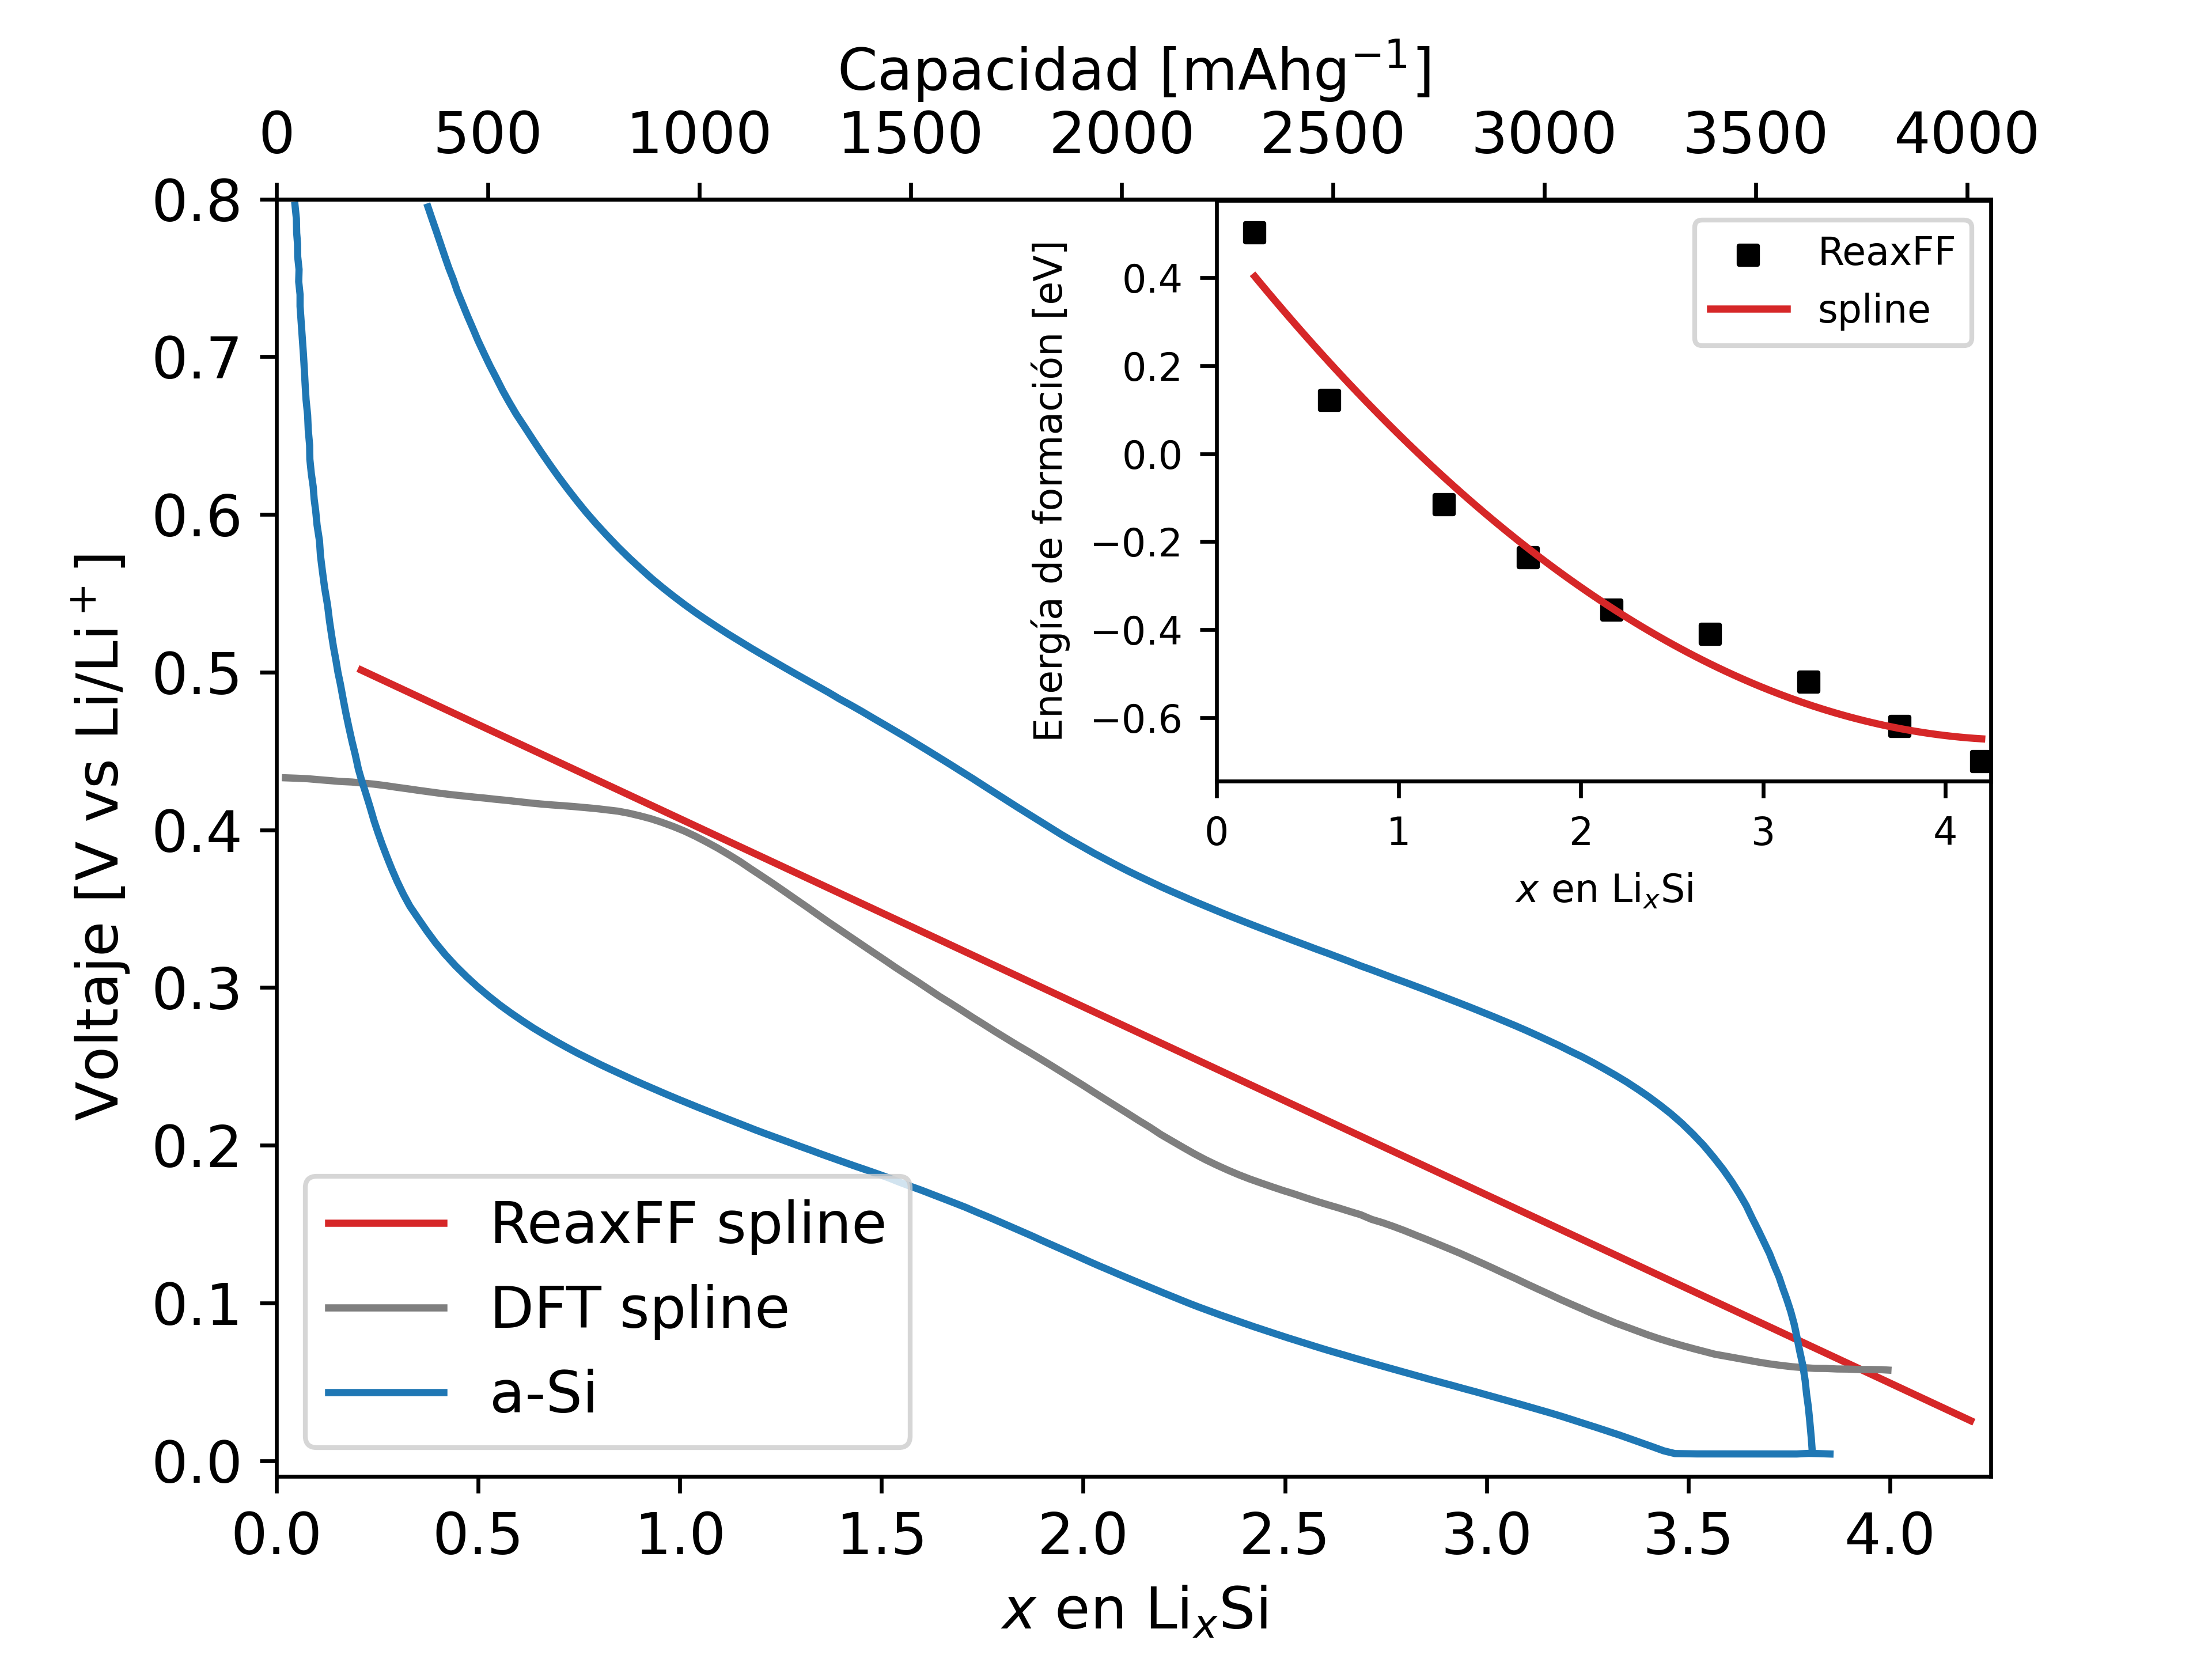
\includegraphics[width=0.8\textwidth]{Silicio/caracterizacion/resultados/electroquimica/voltaje.png}
    \caption{Curvas potencial-concentración para la litiación de ánodos de Si.
    La línea negra corresponde a cálculos de DFT, las líneas azules a 
    curvas medidas experimentalmente en la litiación de Si amorfo y la línea 
    roja es la derivada del \textit{spline} ajustado a los datos de la energía 
    de formación obtenidos con el ReaxFF, presentados en el recuadro.}
    \label{fig:voltaje}
\end{figure}


\subsection{Amorfización del silicio mediante un templado simulado y análisis de la función de distribución radial (RDF)}\label{s:rdfb}

Por último, las mayores discrepancias entre las energías de formación calculadas con DFTB
con respecto a DFT se corresponden a estructuras de silicio amorfo, por lo cual,
se realizó una evaluación extra para este caso. En la Figura \ref{fig:rdfb} se 
muestran las RDFs Si-Si (ver ecuación \ref{eq:rdf}) obtenidas por un templado simulado para cada una de las
parametrizaciones. Además, se compara con el potencial previo de ReaxFF 
\cite{fan2013} y con una determinación experimental \cite{laaziri1999}. Para 
obtener las estructuras amorfas se comenzó con una celda de c-Si con 64 átomos 
a la cual se le realizó un templado simulado en el ensamble $NVT$ utilizando el 
termostato de Nosé-Hoover. El mismo consistió en una etapa inicial de 
calentamiento lineal desde temperatura ambiente hasta 3000 K durante 100 ps, luego una
termalización a dicha temperatura por 600 ps y, por último, un enfriamiento 
exponencial de 600 ps hasta llegar a temperatura ambiente. Para todas las etapas
se utilizó un paso temporal de 1 fs. Para el cómputo de las RDFs que se muestran
en la Figura \ref{fig:rdfb} se equilibró la estructura alcanzada a temperatura 
ambiente durante 100 ps. Puede destacarse que los resultados del conjunto B de parámetros muestran
una concordancia excelente con los datos experimentales de la referencia 
\cite{laaziri1999}, lo que convierte a esta parametrización en la más adecuada
para simulaciones futuras. Los archivos de dichos parámetros están disponibles
en un repositorio público \cite{dftb_lisi}.
\begin{figure}[h!]
    \centering
    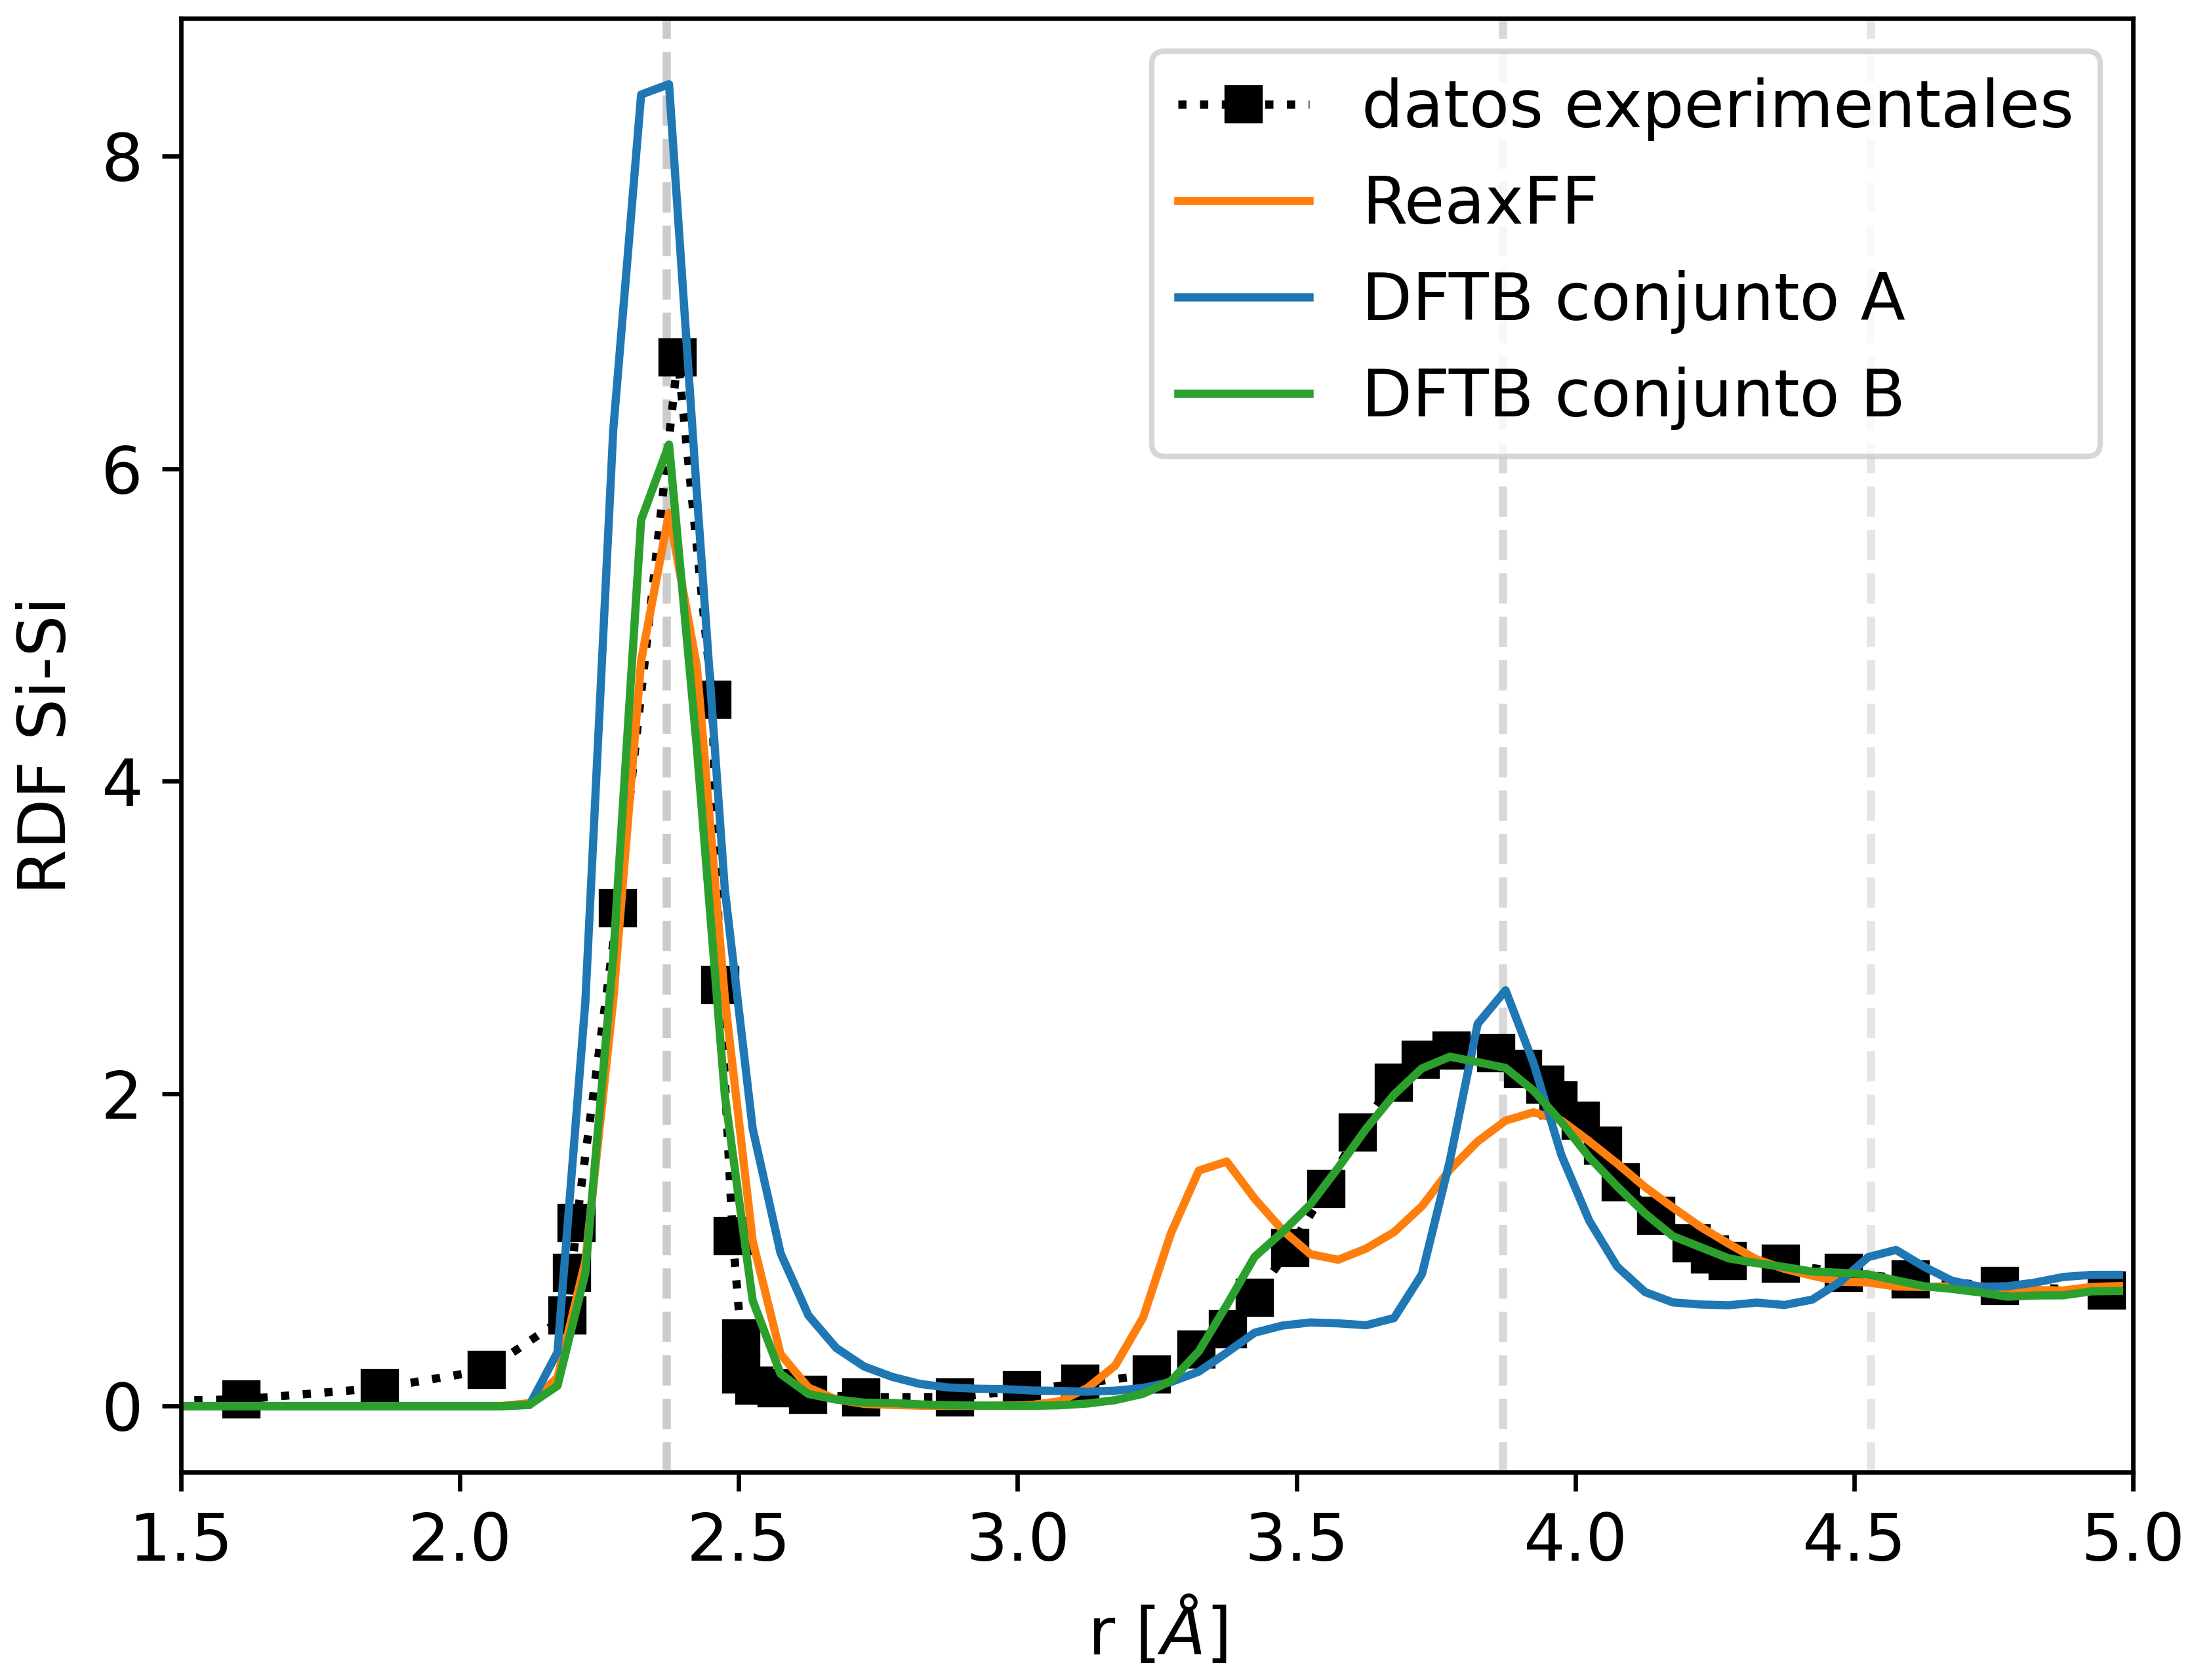
\includegraphics[width=.7\textwidth]{Silicio/modelo/resultados/rdf/rdf.png}
    \caption{Función de distribución radial (RDF) de silicio amorfo para los
    conjuntos A y B de parametrizaciones. Los resultados se comparan con 
    mediciones de la referencia \cite{laaziri1999} y con los resultados obtenidos
    utilizando el ReaxFF \cite{fan2013}. Las líneas grises discontinuas verticales
    muestran dónde estarían los picos del silicio cristalino a 0 K. Se encuentra 
    una concordancia excelente entre el experimento y la parametrización del 
    conjunto B.}
    \label{fig:rdfb}
\end{figure}


% Copyright (c) 2024, Francisco Fernandez
% License: CC BY-SA 4.0
%   https://github.com/fernandezfran/thesis/blob/main/LICENSE
\subsection{Número de coordinación}

De la misma manera que se utilizaron las distribuciones radiales parciales, se pueden
obtener los números de coordinación para un dado tipo de átomo utilizando la ecuación
\ref{eq:cn} definida en la sección \ref{ss:cn} con la $g(r)$ correspondiente. Debido
a que en los materiales amorfos la primera y la segunda esfera de coordinación pueden 
llegar a estar superpuestas, el límite superior de integración no está definido 
unívocamente para todas las concentraciones consideradas \cite{lamparter1995}.
El número de coordinación promedio para átomos de Si vecinos de otros átomos 
de Si se calculó utilizando un radio de 
corte de 3 \AA. Lo mismo se realizó para Li-Li definiendo un radio de corte de 
4 \AA. Para el caso de Si-Li se utilizó el criterio de considerar como radio de 
corte el valor $r$ para el cual la $g(r)$ presenta un mínimo entre los dos picos
a primeros y segundo vecinos. Los resultados se muestran en la Figura 
\ref{fig:cn}a.
\begin{figure}[h!]
    \centering
    \includegraphics[width=\textwidth]{Silicio/caracterizacion/resultados/cn/cn.png}
    \caption{Número de coordinación en función de la concentración de litio para
    Li-Li, Si-Si y Si-Li. Como radios de corte se utilizaron las distancias 
    del pico de la RDF correspondiente. En los casos en que no se aprecia la barra
    de error, la misma es menor que el tamaño de los puntos. (a) Primero número 
    de coordinación. (b) Segundo número de coordinación.}
    \label{fig:cn}
\end{figure}

Para el caso del CN$_{\text{Si}-\text{Si}}$, se tiene que esta cantidad decrece de 4 a 2, a 
medida que la concentración de Li aumenta. Esto indica que a valores pequeños de 
$x$ la estructura de Si mantiene sus conexiones tetraédricas, mientras que para
valores grandes de $x$ el Si tiende a formar cadenas periódicas unidimensionales.
En la red de silicio amorfa, analizada con más detalle en la sección 
\ref{s:clusters}, se presenta una estructura 3d-periódica para valores bajos de 
$x$, donde el CN se encuentra alrededor de 4. Luego, se alcanza una estructura 1d-periódica 
para valores grandes de $x$, donde los enlaces Si-Si tienden a formar 
cadenas, que pueden verse para $x = 3.75$ donde se tiene CN = 2.05, por ejemplo.
El CN de Si-Li y Li-Li presenta valores pequeños para concentraciones 
bajas y aumenta monótonamente hasta alcanzar valores de 10 y 12, respectivamente, 
que se asemejan al valor de una estructura de empaquetamiento compacto.

Los resultados para el segundo número de coordinación se presentan en la Figura 
\ref{fig:cn}b. Estos resultados se obtuvieron considerando un cascarón con un 
radio de corte interno y otro externo, elegidos de manera tal que incluyan el 
segundo pico de la RDF. La elección de dichos valores varió dependiendo del tipo
de átomos que se consideraron. En todos ellos se tomó como radio de corte interno 
el radio de corte del primero número de coordinación. Luego, para el radio de 
corte externo se utilizaron valores de 5.0 \AA\ para Si-Si y 6.0 \AA\ para Li-Li
y Si-Li.

Para los valores de CN$_{\text{Si}-\text{Si}}$ se observa un aumento para concentraciones bajas
de Li, si se lo compara con el CN de primeros vecinos. Para valores mayores de $x$,
se puede ver cómo el valor de CN también tiende a 2, lo cual es coherente con la
formación de cadenas que se notó previamente. La tendencia cualitativa del segundo
CN para Li-Li y Si-Li es la misma que la observada en el primer CN, sólo que ahora
empieza en un valor cercano a 5 y tiende a 35 y 40, respectivamente. Este valor 
es mucho mayor que el que se tiene para los segundos vecinos en una estructura 
de empaquetamiento compacto, que es 6 para la estructura cristalina FCC. Incluso 
es mayor a la suma del segundo (6) y del tercer vecino (24) esperado para la red 
FCC.


% Copyright (c) 2024, Francisco Fernandez
% License: CC BY-SA 4.0
%   https://github.com/fernandezfran/thesis/blob/main/LICENSE
\subsection{Formación de conglomerados (clusters)}\label{s:clusters}

Analizando la formación de \change{conglomerados} (clusters) por medio del algoritmo DBSCAN 
\cite{ester1996}, en el cual puede definirse un radio de corte para el cual se 
deja de considerar que los átomos están enlazados entre sí (es decir, formando 
clusters), se encuentra que las estructuras amorfas de silicio no pueden ser 
clasificadas en diferentes tipos de clusters, las mismas reflejan más bien 
una red amorfa. Esto viene de interpretar los gráficos que se presentan en la 
Figura \ref{fig:clusters}. 
\begin{figure}[h!]
    \centering
    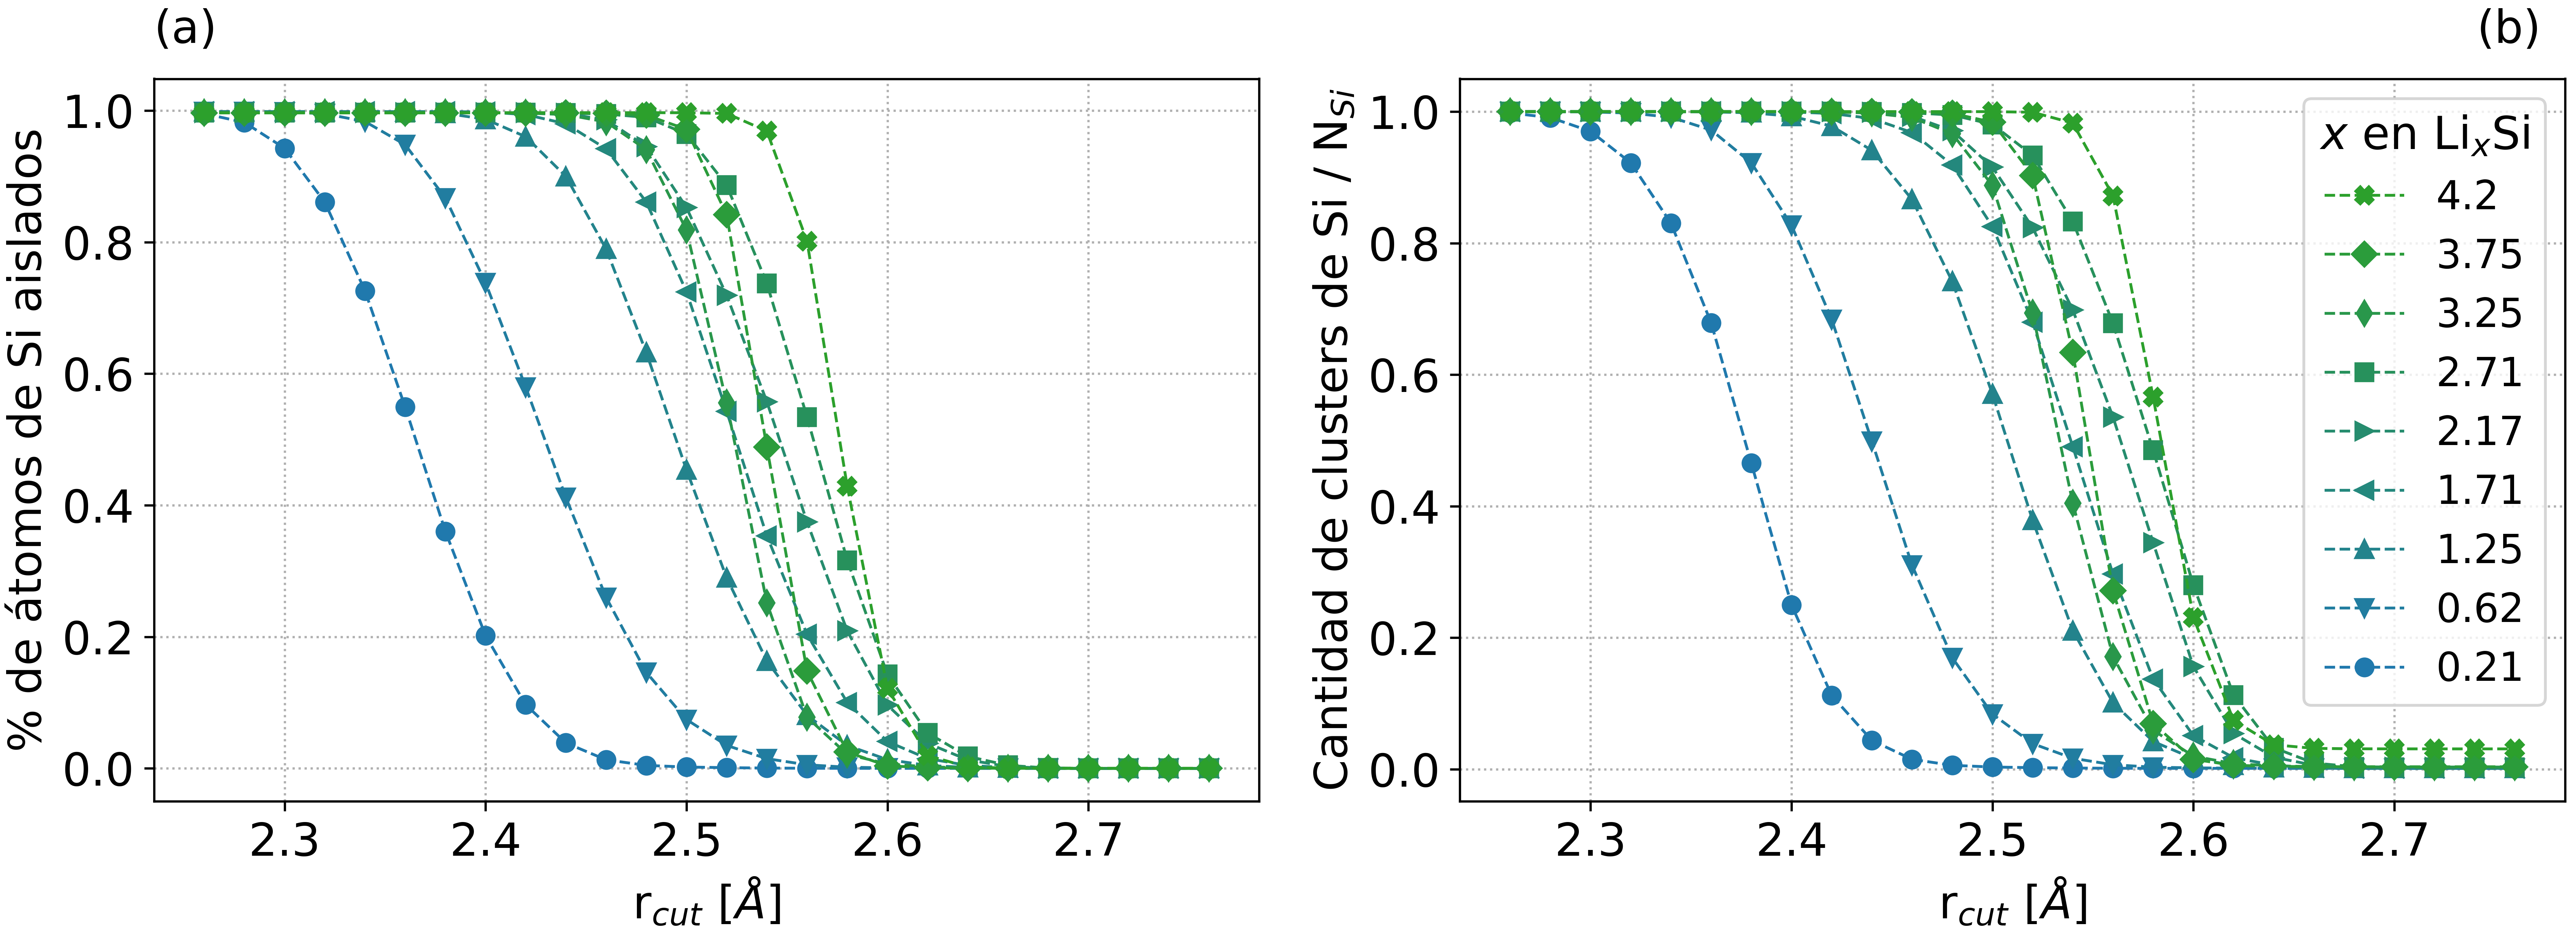
\includegraphics[width=\textwidth]{Silicio/caracterizacion/resultados/clusters/clusters.png}
    \caption{Formación de clusters indicando una red amorfa de silicio. (a) 
    Fracción de átomos de Si aislados en función de la elección del
    radio de corte. (b) Número de clusters de Si sobre el número total de átomos 
    de Si.}
    \label{fig:clusters}
\end{figure}

En particular, en la Figura \ref{fig:clusters}a se define la fracción 
de átomos de Si que están a una distancia mayor que $r_{cut}$ de otros átomos de 
Si. Cuando el radio de corte es mayor que la distancia a la cual termina el 
primer pico de la RDF$_{\text{Si}-\text{Si}}$, no se tienen átomos de Si que cumplan esta 
propiedad, es decir, no hay átomos de Si que se encuentren aislados en el sistema,
incluso a concentraciones altas de Li. Esto refleja que el a-Si se comporta como 
una red en la cual todos los átomos de silicio están interconectados entre sí, 
cosa que también se puede deducir de la Figura \ref{fig:clusters}b, en la cual 
se tiene que cuando el radio de corte es menor que el primer pico de la RDF$_{\text{Si}-\text{Si}}$ 
el número de clusters es igual al número de átomos de Si, pero que cuando este 
radio es más grande que la distancia a la cual termina el primer pico, hay un 
solo cluster.


\subsection{Interconexión de clusters}\label{s:interconexion}

Para determinar qué es lo que genera una estructura compleja en el segundo pico de la 
RDF$_{\text{Si}-\text{Li}}$, ver Figura \ref{fig:rdf}, se realizó un análisis similar al reportado por Ding \textit{et al.}
\cite{ding2015}. Estos autores analizaron la correlación en la distancia de a
pares de los segundos vecinos más cercanos en términos de las conexiones entre
clusters, definiendo un poliedro de coordinación alrededor del átomo central 
considerado para la RDF y sus segundos vecinos. El número de átomos compartidos
entre estos dos poliedros de coordinación enlazados fueron utilizados para 
establecer categorías y analizar sus contribuciones a la RDF. Estas categorías
dependen del hecho de que los poliedros comparten un vértice (1 átomo), una 
arista (2 átomos), una cara de los poliedros (3 átomos) o cuadriláteros 
distorsionados o tetraedros aplastados (4 átomos). De una forma similar al trabajo de Ding, se deconvolucionó el segundo pico de la RDF calculando la RDF parcial 
de distintas categorías, donde cada categoría se define por el número de átomos de
Li que interconectan un átomo de Si con su segundo vecino de Li. El comportamiento
detallado se presenta en la Figura \ref{fig:interconexiones}. Puede afirmarse a 
grandes rasgos que para concentraciones bajas de Li en las aleaciones, hay una 
predominancia de segundos vecinos de Li que tienen una o ninguna interconexión 
con los vecinos de Li de la primera esfera de coordinación Si-Li. Para $x > 1.0$
la contribución del segundo vecino de Li interconectado con dos o más átomos de 
Li de la primera esfera de coordinación Si-Li comienza a ser predominante y la
contribución de los átomos de Li sin conectarse empieza a decaer. Para $x > 3.0$,
la contribución del primer pico del segundo vecino de Li interconectado dos o
tres veces se vuelve relevante mientras que aparecen contribuciones de cuatro o
más interconexiones.
\begin{figure}[h!]
    \centering
    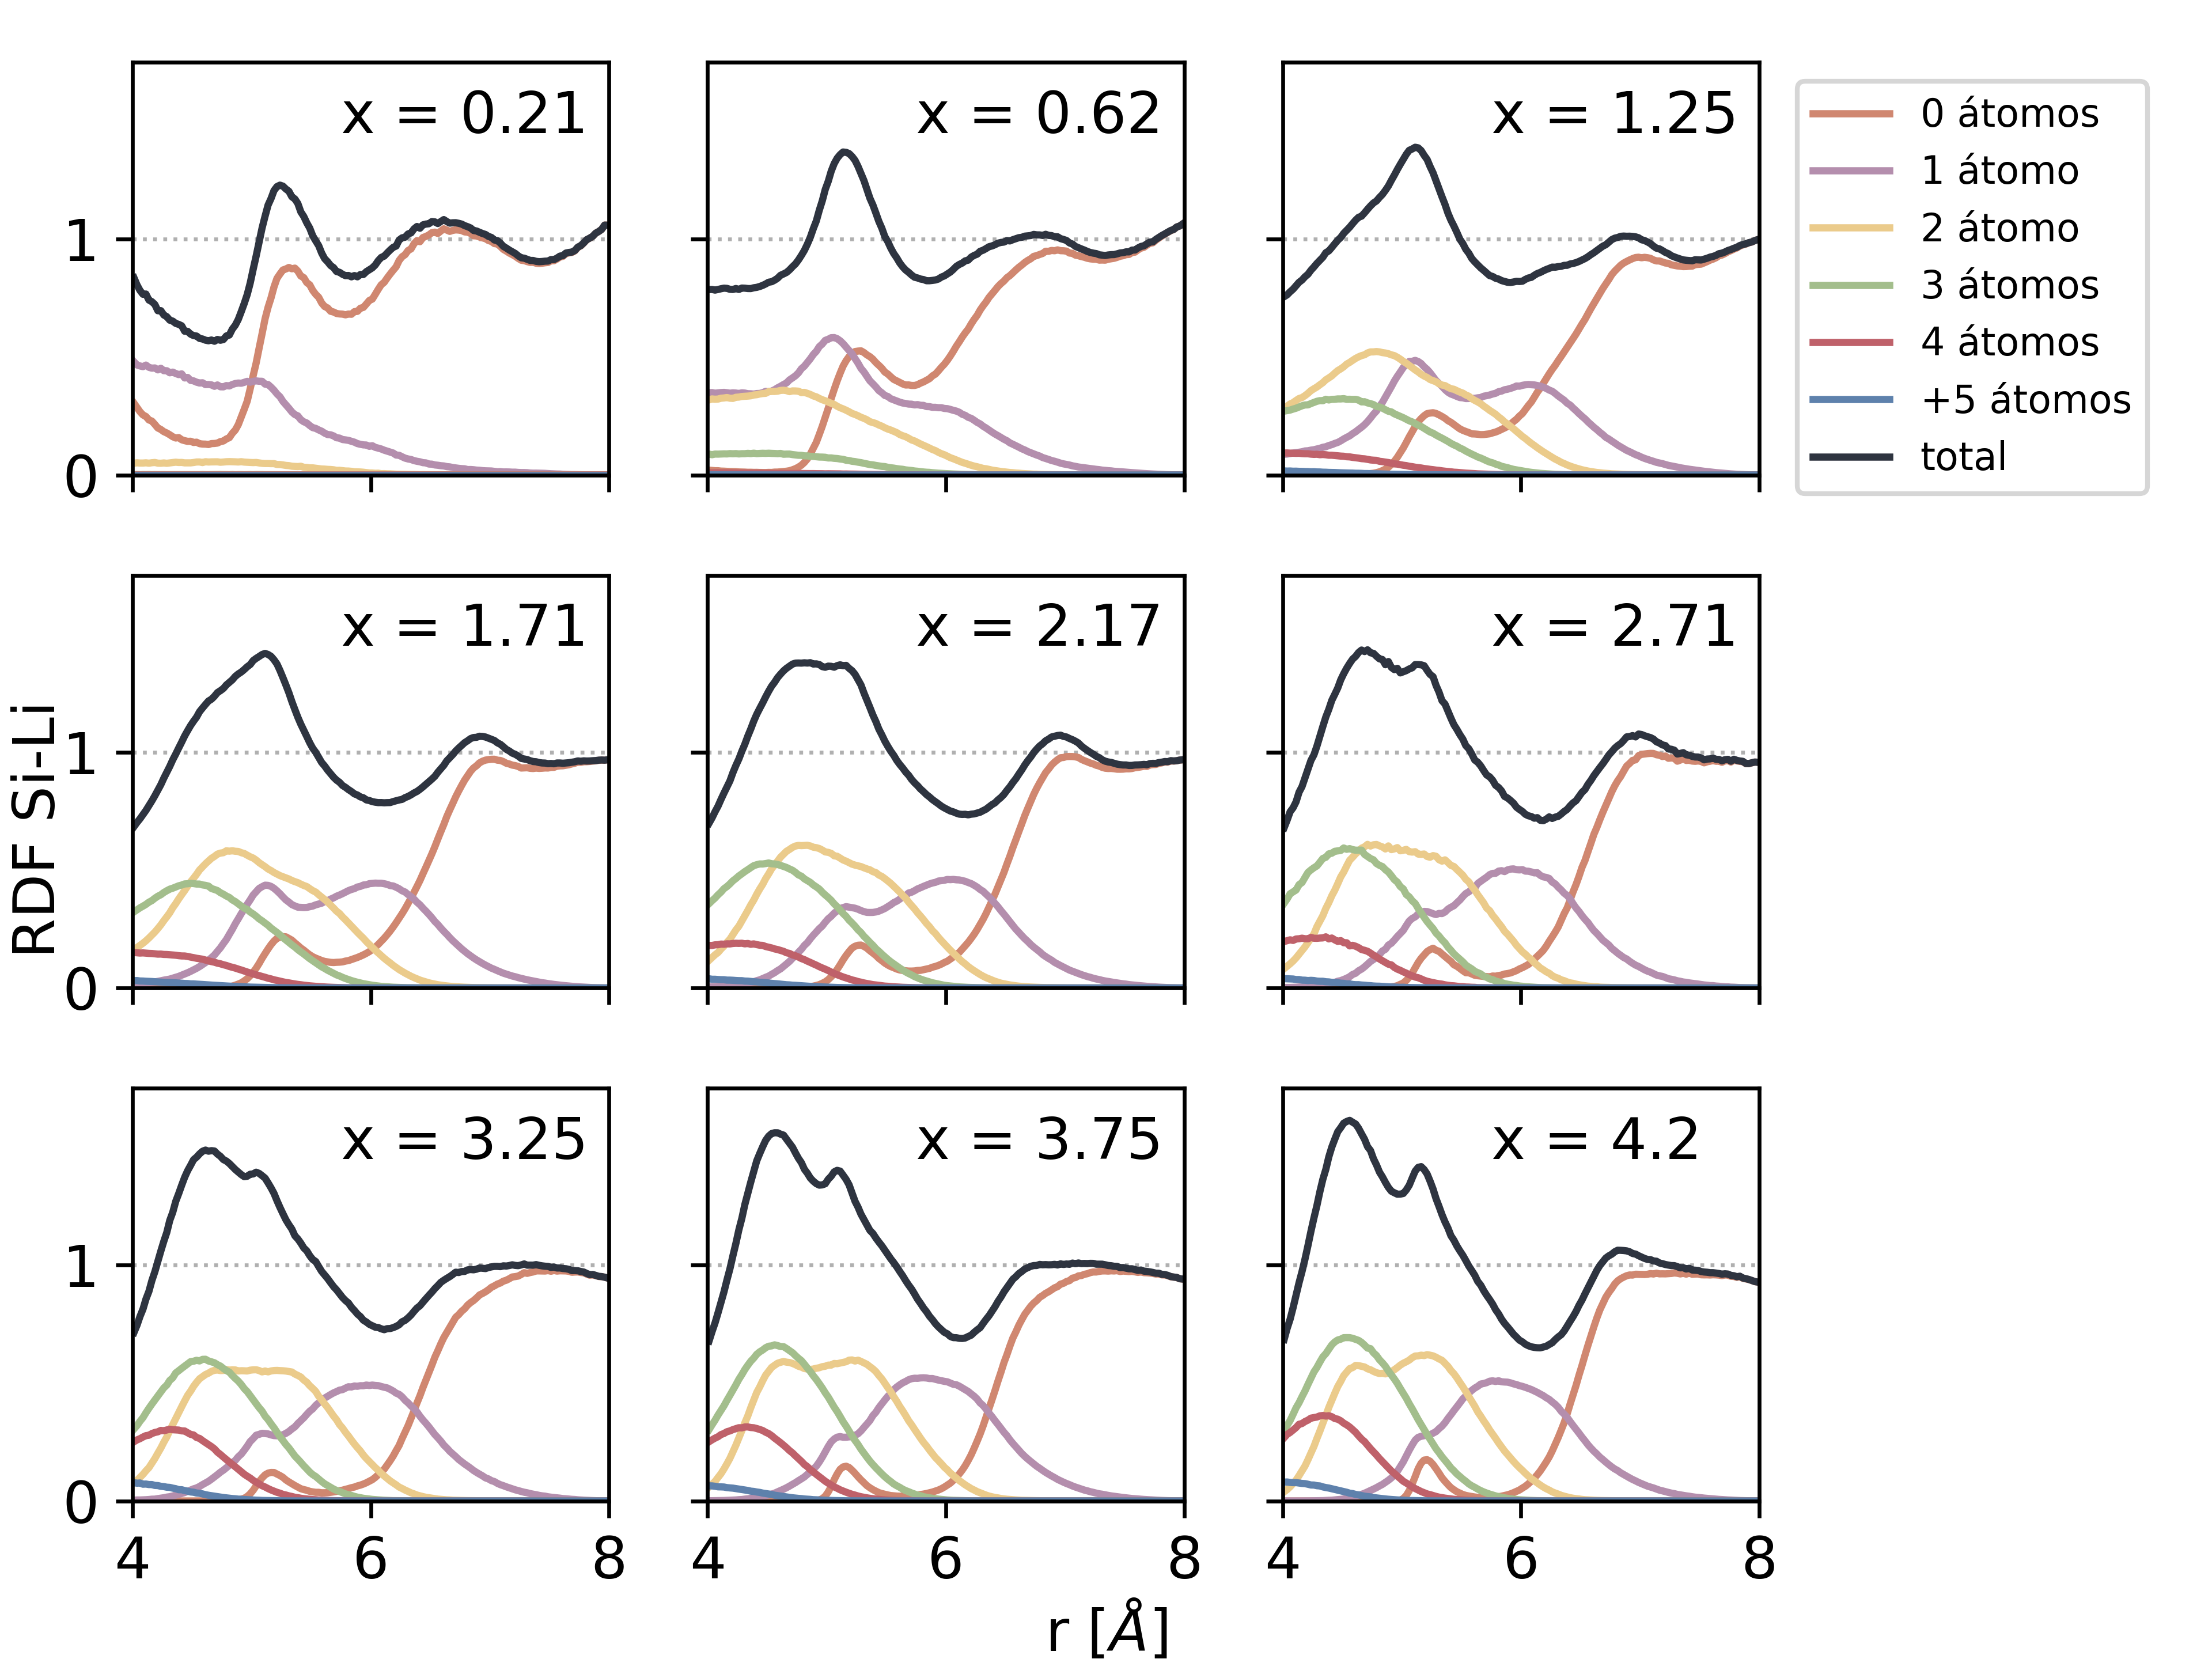
\includegraphics[width=\textwidth]{Silicio/caracterizacion/resultados/interconexion/interconexiones.png}
    \caption{Interconexiones de los segundos vecinos más cercanos de Li con un 
    átomo central de Si para cada valor de $x$ en Li$_x$Si considerado \cite{ding2015}. El número 
    de primeros vecinos más cercanos que conectan a los segundos vecinos más 
    cercanos con el átomo central de Si se indica en el recuadro de las figuras. 
    Además de la RDF$_{\text{Si}-\text{Li}}$ total, se grafica cada una de las contribuciones 
    de los diferentes tipos de interconexiones posibles.}
    \label{fig:interconexiones}
\end{figure}

Mientras que el comportamiento presentado en la Figura \ref{fig:interconexiones}
es más bien complejo, pueden establecerse tendencias generales que ayudan a 
entender mejor que es lo que sucede. Si se divide la RDF$_{\text{Si}-\text{Li}}$ en dos 
contribuciones de segundos vecinos, la primera de ellas, que se encuentra a una
distancia entre 4.0 \AA\ y 5.0 \AA, se puede atribuir a los átomos que tienen dos 
o más interconexiones de Li, mientras que la segunda de ellas, entre 5.0 \AA\ y
5.6 \AA, se corresponde con los átomos que tiene una o ninguna interconexión de 
Li. Utilizando esta clasificación, se muestra en la Figura 
\ref{fig:interconexiones-areas} la fracción del área que representa cada una de
estas categorías en función de la concentración de litio.
\begin{figure}[h!]
    \centering
    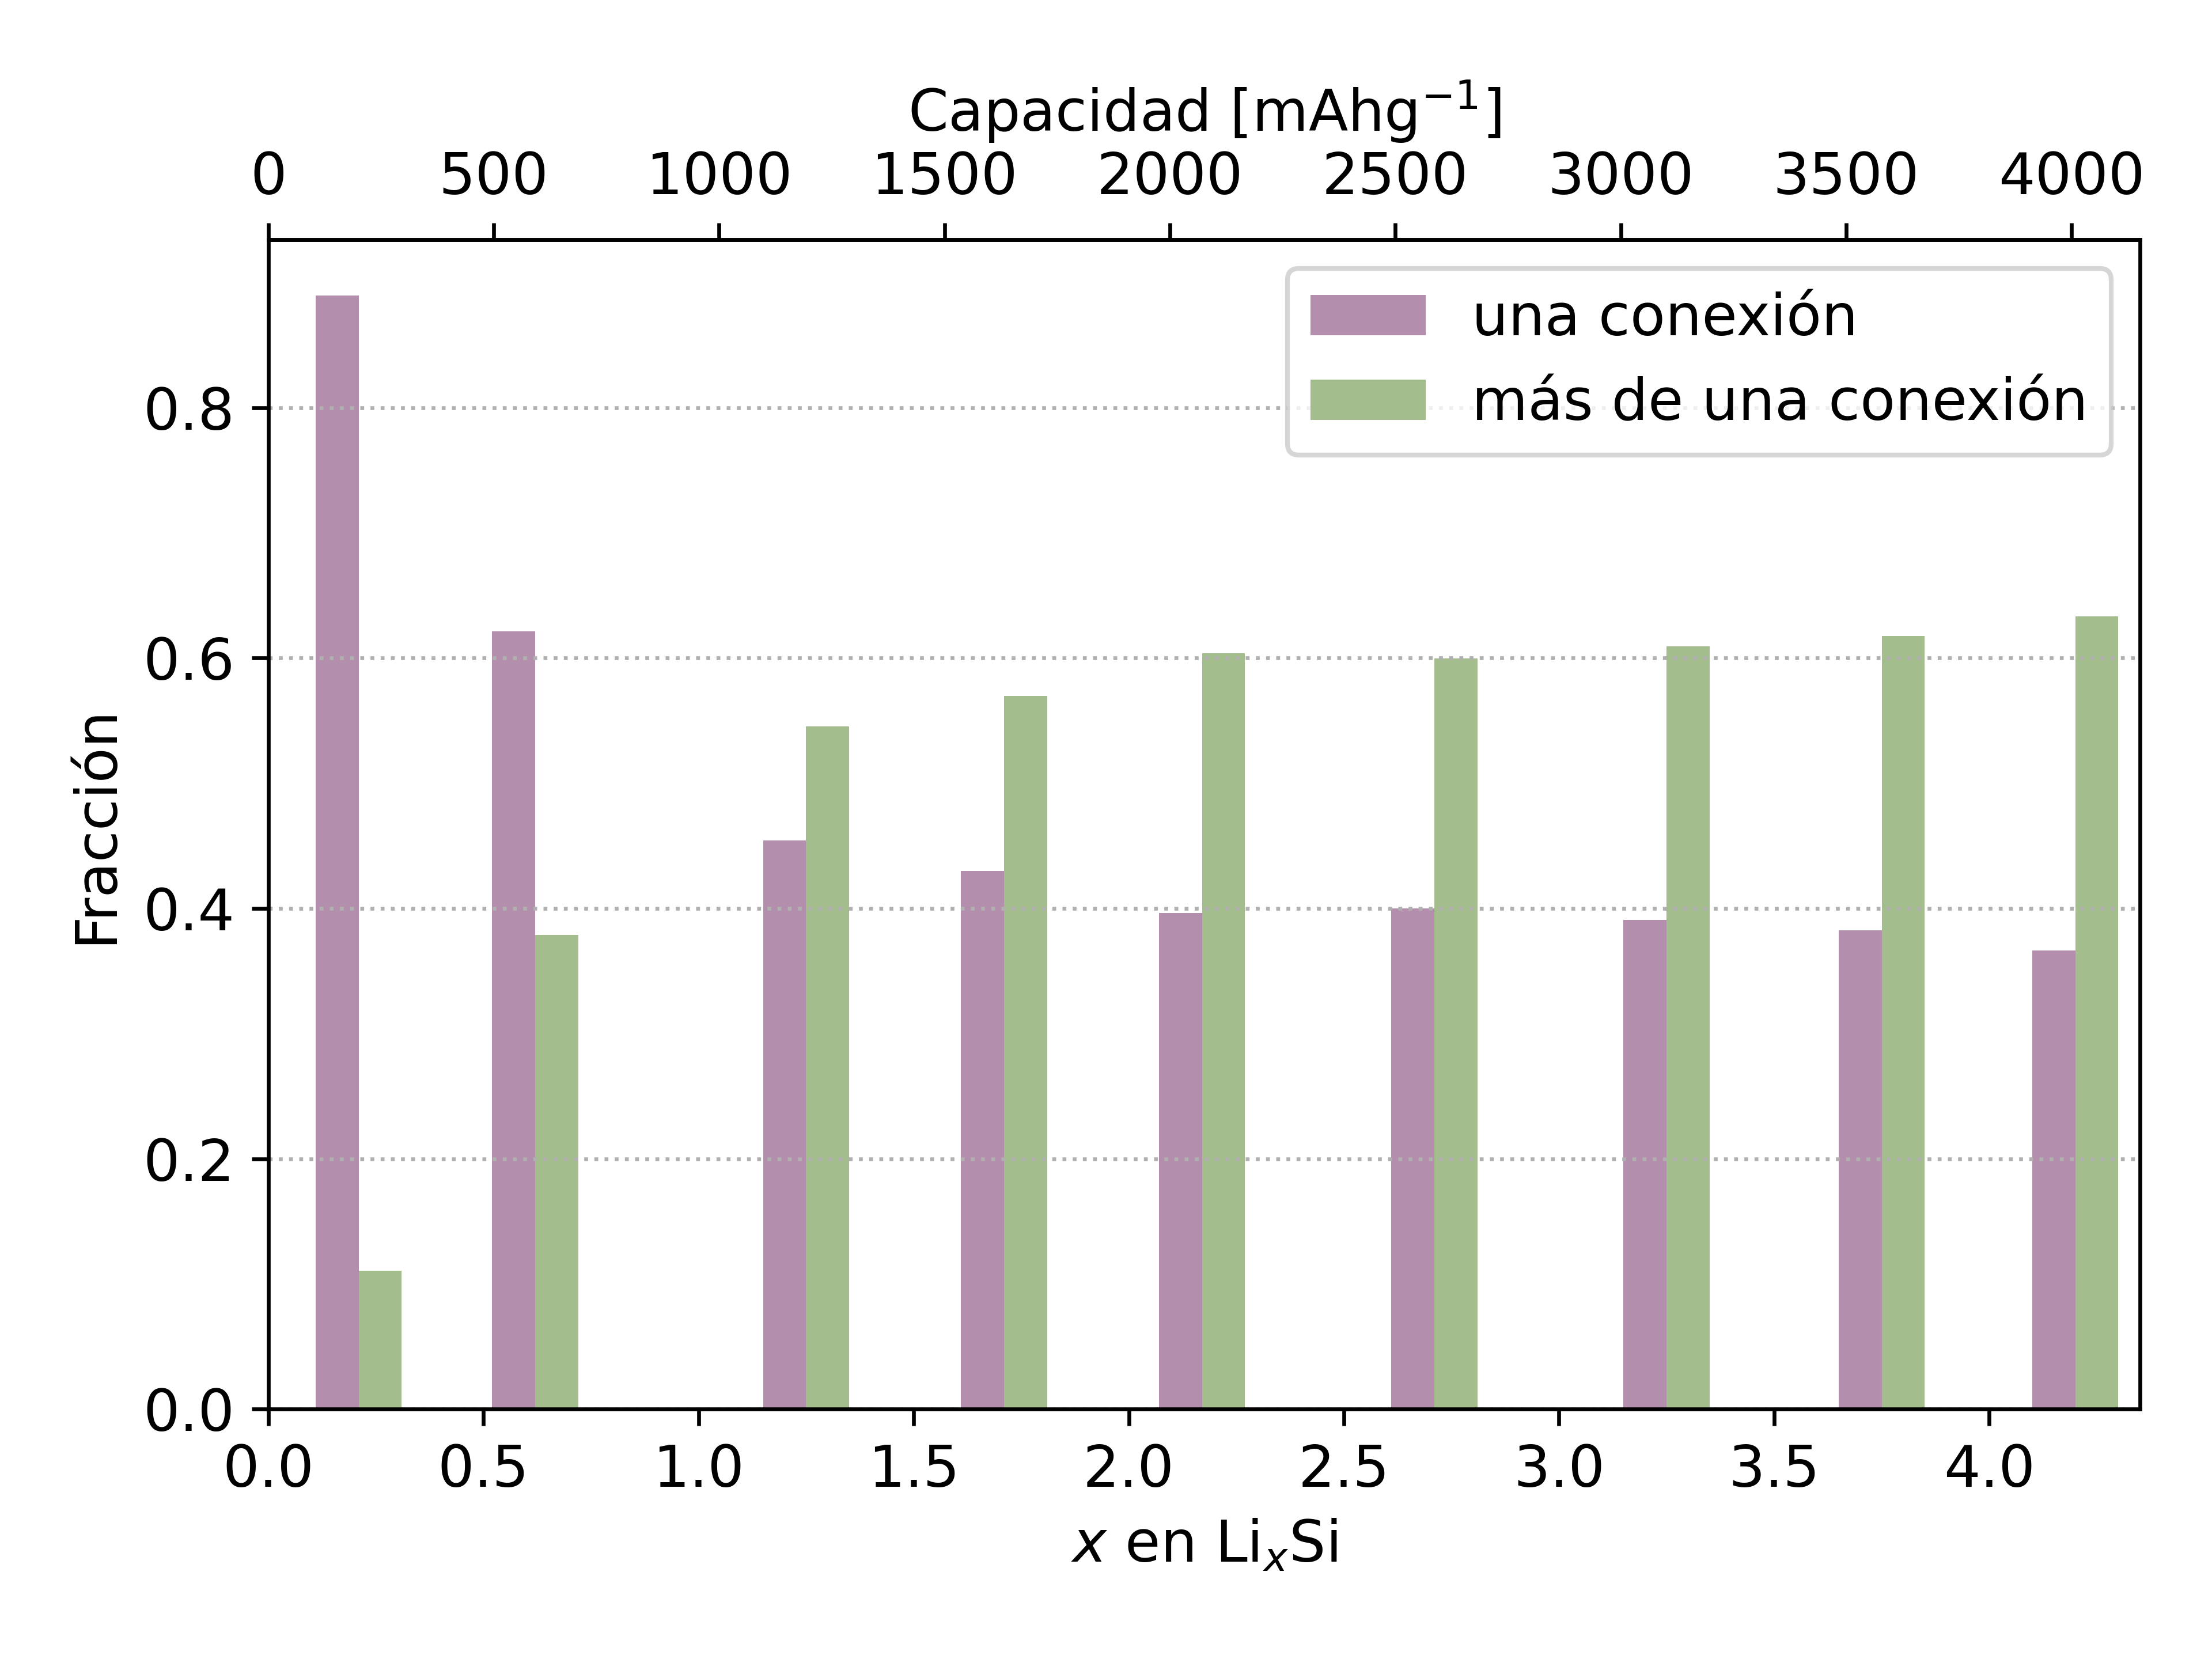
\includegraphics[width=0.7\textwidth]{Silicio/caracterizacion/resultados/interconexion/interconexiones-areas.png}
    \caption{Evolución con la concentración de la fracción que representa cada
    categoría de interconexiones de Li al área total del segundo pico de la 
    RDF$_{Si-Li}$.}
    \label{fig:interconexiones-areas}
\end{figure}


\subsection{Orden de corto alcance}

El término orden de corto alcance (SRO, de sus siglas en inglés 
\textit{short-range order}) se utiliza para denotar el ordenamiento de los átomos
que rodean a uno específico en una cáscara. Del mismo modo, el término 
\textit{clustering} se ha definido como la tendencia de los átomos similares a 
estar cerca unos de otros. Ambos conceptos se refieren a un orden estructural 
entre átomos vecinos, pero no son necesariamente persistentes a distancias más 
largas. Warren ~\cite{warren69} y Cowley ~\cite{cowley1950} definieron un 
parámetro (WCP) para caracterizar estos tipos de ordenamientos de la siguiente 
manera:
\begin{equation}
    WCP = 1 - \frac{p_{A-B}}{m_B} = 1 - \frac{p_{B-A}}{m_A},
\end{equation}
donde $p_{A-B}(p_{B-A})$ es la probabilidad de tener un átomo de tipo B(A) como
vecino de un átomo de tipo A(B) y $m_B(m_A)$ es la concentración global de átomos
B(A), expresadas en fracciones molares. La igualdad, en ambas definiciones 
posibles del WCP, viene del hecho de que la probabilidad de encontrar a un átomo 
de tipo A como vecino de un átomo de tipo B es igual a la de tener un átomo de 
tipo B como vecino de un átomo de tipo A, esto es $m_A p_{A-B} = m_B p_{B-A}$.

Los valores que se obtienen de utilizar el parámetro WCP en sistemas del tipo
A$_x$B indica una aleatoriedad completa si es igual a cero, preferencia por 
átomos de distinto tipo si $WCP < 0$ y preferencia por átomos del mismo tipo si 
$WCP > 0$. Aunque este parámetro permite un análisis cuantitativo notable, sólo
se define para sistemas cristalinos en los que cada átomo tiene el mismo número
de vecinos. ~\cite{warren69}

A continuación se extiende esta idea para definir un nuevo parámetro, 
$\theta_{A-B}$, que es adecuado para caracterizar estructuras amorfas, de la 
siguiente manera:
\begin{equation}
    \theta_{A-B} = \ln \left( \frac{C_{A-B}}{C_{Bulk}} \right),
\end{equation}
donde A indica la naturaleza del átomo que se considera como central y B el tipo
de átomo que se considera como vecino, equivalente a la definición de WCP. En
este caso, la relación entre la concentración local y la concentración global se 
calcula a partir de la integración de la distribución radial de a pares parcial,
$g_{A-B}(r)$, en una esfera al rededor del átomo central,
\begin{equation}
    \frac{C_{A-B}}{C_{Bulk}} = \frac{1}{V(r_{cut})} \int_0^{r_{cut}} g_{A-B}(r) dV,
\end{equation}
donde $r_{cut}$ y $V(r_{cut})$ son el radio de corte y el volumen de la esfera 
considerada. Ya que en $g_{A-B}(r)$ no hay dependencia angular, $dV$ puede 
escribirse como $4 \pi r^2 dr$. Esta cantidad puede pensarse como la 
concentración promedio dentro de la esfera relativa a la del material 
masivo. Así, de forma análoga al parámetro de WCP, $\theta_{A-B}$ indica 
la tendencia SRO o el \textit{clustering} para cualquier tipo de átomo dado.
Si $\theta$ es positivo, indica una acumulación de átomos relativa al 
\textit{bulk}, mientras que si es negativo indica una disminución. Si es igual a 
cero se tiene una aleatoriedad completa. Este nuevo parámetro también satisface 
la relación $\theta_{A-B} = \theta_{B-A}$ de la misma manera que se discutió para
el parámetro de WCP, ya que por definición $g_{A-B}(r) = g_{B-A}(r)$. Por lo cual 
se tiene que el parámetro $\theta_{A-B}$ da información similar a la que provee 
el WCP, pero además es aplicable a sistemas amorfos.

La figura \ref{fig:sro} muestra la variación del parámetro $\theta$ en función 
de la concentración de Li. Hay tres posibilidades para el análisis de $\theta$ en
sistemas de Li$_x$Si ($\theta_{Li-Li}$, $\theta_{Si-Si}$ y $\theta_{Si-Li}$), ya
que $\theta_{Si-Li} = \theta_{Li-Si}$. Para todos los casos se consideraron los
mismos radios de corte que en los cálculos del número de coordinación, luego del
primer pico de la RDF correspondiente.
\begin{figure}[th]
    \centering
    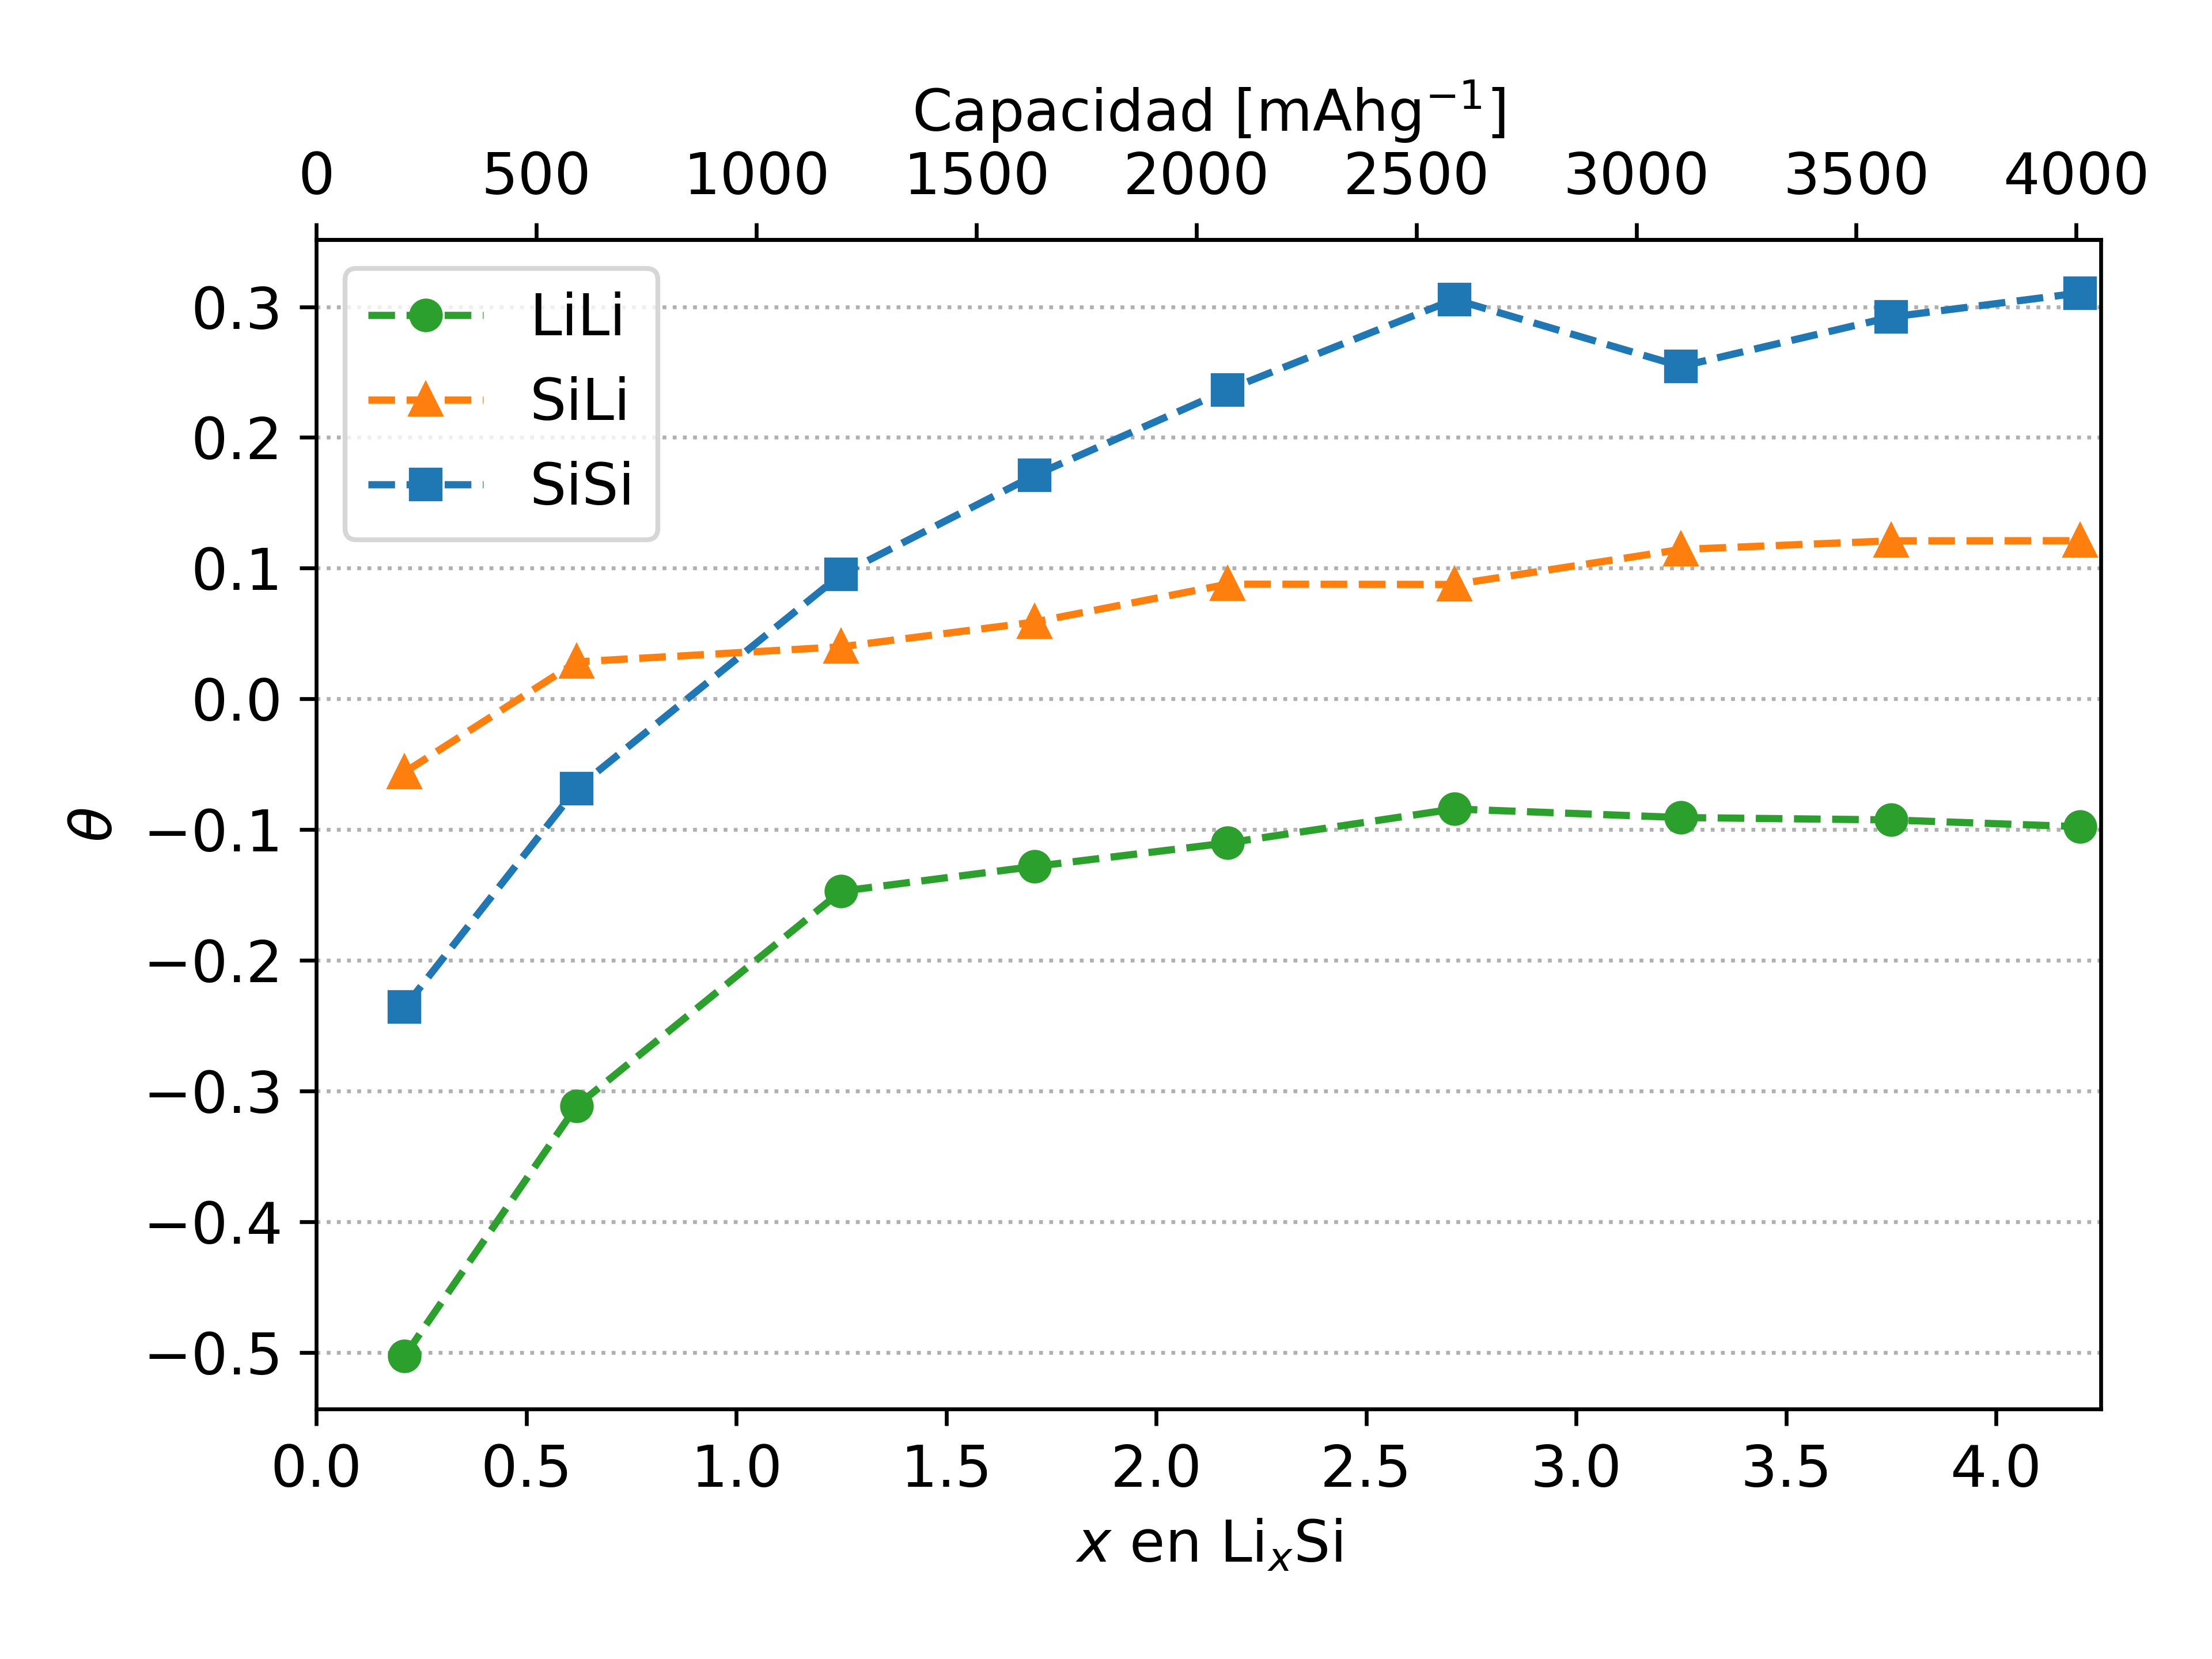
\includegraphics[width=0.8\textwidth]{Silicio/caracterizacion/resultados/sro/sro.png}
    \caption{Parámetros $\theta_{Li-Li}$, $\theta_{Si-Li}$ y $\theta_{Si-Si}$ 
    en función de la concentración de Li. El primer subíndice indica el tipo de
    átomo que se considera como central mientras que el segundo es el vecino. El
    radio de corte se eligió luego del primer pico de la RDF correspondiente.}
    \label{fig:sro}
\end{figure}

Como tendencia general, puede notarse que todos los valores de $\theta$ aumentan
cuando crece la cantidad de litio en el sistema, $x$, y que se estabiliza para 
valores grandes de $x$. Este comportamiento monótono y la disminución en la 
pendiente para concentraciones altas está correlacionado con el comportamiento
presentado en el análisis de los números de coordinación.

En el caso de $\theta_{Si-Si}$, alcanza un valor positivo aproximadamente 
constante para $x > 2.5$, mostrando una correlación fuerte con la presencia de 
cadenas lineales de Si, previamente discutidas y observadas en la figura 
\ref{fig:amorfas}. Aunque la presencia de estas cadenas se puede inferir a partir
de los valores de los CN en $x$ altos, $\theta$ es más sensible al SRO, ya que
está normalizado por la concentración global. Esta propiedad de $\theta$ permite
un análisis más claro incluso si las cadenas están interactuando entre sí, como
es el caso para concentraciones bajas de litio.

$\theta_{Si-Li}$ presenta variaciones pequeñas y un valor positivo para todo 
$x > 0.5$, mostrando una acumulación constante de Li al rededor del Si, o, 
análogamente, una acumulación de Si alrededor del Li. Este comportamiento se le 
puede atribuir a la interacción atractiva fuerte en los pares Si-Li. En el caso de 
$\theta_{Li-Li}$, este parámetro es siempre negativo, lo que indica una 
interacción débil Li-Li y la correspondiente disminución de vecinos Li-Li. Por
último, el parámetro $\theta_{Si-Si}$ tiene un valor negativo para $x < 1.0$, 
sugiriendo que la presencia de concentraciones bajas de litio tiende a separar 
los átomos de silicio entre sí. Sin embargo, $\theta_{Si-Si}$ se vuelve positivo
para $x > 1.0$, implicando una acumulación de vecinos de Si sobre átomos de Si, 
relativo a la concentración global. Esto se debe a la formación de estructuras 
Si-Si. Para $x > 2.5$ puede observarse un valor constante de 
$\theta_{Si-Si} \approx 0.3$, revelando la formación de estructuras estables de 
Si-Si dadas por las cadenas previamente mencionadas.




%
%\part{Conclusiones generales}
%
%

% Apéndices
% \part{Apéndices}

% \appendix
% \renewcommand\chaptername{Apéndice}
% \chapter{Software desarrollado}

En la última década, Python se ha convertido en un lenguaje de programación 
importante dentro de la comunidad científica debido a su facilidad de uso y 
versatilidad en la manipulación y visualización de datos ~\cite{millman2011}. 
Por lo tanto, los software diseñados en esta tesis han sido escritos en este
lenguaje y construidos sobre las librerías usuales del cómputo científico como
NumPy \cite{numpy}, SciPy \cite{scipy}, pandas \cite{pandas}, 
matplotlib \cite{matplotlib} y scikit-learn \cite{sklearn1, sklearn2}. 


\section{Control de calidad de software}

El control de calidad del software hace referencia al conjunto de reglas y 
procedimientos que deben utilizarse para verificar que el software cumple 
determinados estándares de calidad subjetivos. Un procedimiento habitual son las 
pruebas unitarias (\textit{unit testing} en inglés), que consisten en aislar una 
función del código y comprobar que funciona como se espera \cite{jazayeri2007}. 
Otro procedimiento habitual se define a partir de este y es el 
\textit{code-coverage}, que determina que proporción del software se ha testeado
\cite{miller1963}. El estilo y la legibilidad del código también es importante
y aquí se ha seguido la guía de estilo PEP8 de Python, la misma se asegura con 
la herramienta flake8. Además, los mismos fueron desarrollados utilizando control 
de versiones git y distribuidos bajo la Licencia MIT, fomentando su uso tanto en 
entornos académicos como comerciales. Todo esto se realizó buscando que el 
software sea fácil de mantener y que respete los estándares de la comunidad Python.


\section{galpynostatic}

Este paquete denominado \path{galpynostatic} fue escrito para la utilización
del modelo heurístico presentado en el capítulo TODO. El mismo distribuye los 
datos de los diagramas galvanostáticos, un módulo de preprocesamiento de datos
para obtener capacidades de descarga a un potencial de corte dado a partir de 
medidas de perfiles galvanostáticos y una clase que realiza la regresión sobre la 
superficie y permite diferentes tipos de gráficos y estimaciones de parámetros.

A continuación se muestra un ejemplo de uso:

\lstinputlisting[language=Python]{apendices/ejemplo_galpynostatic.py}

A \path{galpynostatic} se le realizan múltiples pruebas unitarias sobre datos de
de electrodos actuales y de materiales de investigación de próxima generación en 
baterías de litio, el \textit{coverage} del mismo alcanza el 100\% del software
en su versión inicial.

Por último, el código fuente está disponible en un repositorio público 
(\url{https://github.com/fernandezfran/galpynostatic}) y todos los nuevos cambios 
confirmados en este repositorio se prueban automáticamente con el servicio de 
integración continua de GitHub Actions. También se genera una documentación a 
partir de los docstrings del código, junto con una guía de instalación,
tutoriales y ejemplos con aplicaciones reales, que se hacen públicos en el 
servicio read-the-docs (\url{https://galpynostatic.readthedocs.io/en/latest/}). 
Además, \path{galpynostatic} está disponible para su instalación en el Python 
Package-Index (\url{https://pypi.org/project/galpynostatic/}).

%
%\section{galpynostatic.metric}
%
%TODO
%
%
%\section{macchiato}
%
%TODO
%
%Ejemplo de cálculo del corrimiento químico de la estructura cristalina 
%Li$_{13}$Si$_{4}$ mediante el uso del modelo a primeros vecinos introducido en 
%el capítulo TODO:
%\lstinputlisting[language=Python]{apendices/ejemplo_macchiato.py}
%
%
%\section{Otros códigos}
%
%\subsection{sierras}
%Con \path{sierras} se automatiza el proceso de ajustar la ecuación de Arrhenius 
%(\ref{eq:arrhenius}) en procesos difusivos y la obtención de información a partir 
%de la misma. Este código también se encuentra público 
%(\url{https://github.com/fernandezfran/sierras}) y cada vez que se realiza un 
%cambio se llevan a cabos tests unitarios sobre distintos datos extraídos de 
%literatura. Un ejemplo simple de como se utiliza se presenta a continuación:
%
%\lstinputlisting[language=Python]{apendices/ejemplo_sierras.py}
%
%La versión inicial de este código fue presentada como trabajo final en la materia
%\href{https://github.com/leliel12/diseno_sci_sfw}{\tt Diseño de software para 
%cómputo científico.}
%
%\subsection{exma}
%Para analizar trayectorias de dinámica molecular, dentro de la comunidad de Python
%se encuentra la librería \path{MDAnalysis} \cite{mdanalysis1, mdanalysis2}. Sin
%embargo, no todos los observables descriptos en la sección \ref{s:observables}
%han sido implementados, por ejemplo, no se puede calcular directamente el número
%de coordinación. Para ello se escribió \path{exma}
%(\url{https://github.com/fernandezfran/exma}), que además de contar con esta
%implementación presenta distintas facilidades para computar observables 
%electroquímicos presentados en distintos capítulos de esta tesis. Algunas partes
%de este software han sido escritas en \path{C}, para tener mayor velocidad de 
%cálculo, y tienen una interfaz en Python para ser utilizadas.
%
%\subsection{aelm}
%Para el método de exploración acelerada de mínimos locales, introducido en 
%la sección \ref{s:aelm} del capítulo \ref{ch:caracterizacion}, se escribió un 
%módulo de Python, \path{aelm} (\url{https://github.com/fernandezfran/aelm}), que 
%toma una trayectoria de una dinámica molecular sesgada, minimiza cada uno de los 
%frames con algún programa de dinámica molecular a elección (\path{LAMMPS} o 
%\path{GEMS}, por ejemplo) y guarda las configuraciones atómicas y las energías 
%para su posterior análisis, como se realizó en el capítulo 
%\ref{ch:caracterizacion} ¿o TODO?
%
%\subsection{cluster-connections}
%Se escribió un código en \path{C++}, 
%\url{https://github.com/fernandezfran/cluster-connections}, con un algoritmo de
%\textit{clustering} para deconvolucionar numéricamente el segundo pico de la RDF
%según la cantidad de vecinos que interconectan a segundos vecinos, como se analizó
%en la sección \ref{s:interconexion} del capítulo \ref{ch:caracterizacion}, 
%en la figura \ref{fig:interconexiones}.


\bibliographystyle{apalike}
\bibliography{citas}

\end{document}
